%! TEX TS-program = lualatex
\documentclass[11pt, a4paper]{book}

\usepackage{fontspec}
\usepackage{ifthen}
\usepackage{mathtools}
\usepackage{xurl}
\usepackage{tocloft}
\renewcommand{\cftfigdotsep}{\cftnodots}
\renewcommand{\cfttabdotsep}{\cftnodots}
\renewcommand{\cftfigleader}{\hspace{0.5em}}
\renewcommand{\cftfigfont}{\color{black}}
\renewcommand{\cftfigpagefont}{\itshape}
\renewcommand{\cftfigafterpnum}{\cftparfillskip}
\renewcommand{\cfttableader}{\hspace{0.5em}}
\renewcommand{\cfttabfont}{\color{black}}
\renewcommand{\cfttabpagefont}{\itshape}
\renewcommand{\cfttabafterpnum}{\cftparfillskip}
\renewcommand{\cftpnumalign}{l}
\cftsetrmarg{0em}
\setlength{\cftfigindent}{0em}
\setlength{\cfttabindent}{0em}
\usepackage{etoc}
\usepackage{floatrow}
\usepackage{todonotes}
\usepackage[detect-all=true,mode=match]{siunitx}
\usepackage[linesnumbered, noend, ruled]{algorithm2e}
\usepackage{booktabs}
\usepackage{pdflscape}
% hypcap puts the hyperref to the figure instead of the caption.
% I might want to have a look at this hypcap=false again
% it doesnt seem to work with sidefigures, and using the suggested workaround in
% the caption manual (captionsetup{type=figure}) changes the spacing of the caption for some reason
\usepackage[font=footnotesize,hypcap=false]{caption}
\usepackage{afterpage}
\usepackage{marginfix}
\usepackage[export]{adjustbox}
\usepackage{csquotes}
\usepackage[super]{nth}
\usepackage{etoolbox}
\usepackage{csvsimple-l3}
\usepackage{xfp}
\usepackage{threeparttable}

\usepackage{interval}
\intervalconfig{soft open fences}
\usepackage{multirow}

\usepackage{amssymb}
\usepackage{framed}
\usepackage{mdframed}
\usepackage{amsthm}
\newtheoremstyle{break}
  {\topsep}
  {\topsep}
  {\itshape}
  {0pt}
  {\bfseries}
  {.}
  {\newline}
  {\thmname{#1}\thmnumber{ #2}\thmnote{ \textbf{(#3)}}}
\newmdtheoremenv[
  linecolor=black,
  innertopmargin=0pt,
  innerbottommargin=10pt,
]{lemma}{Lemma}[section]
\newmdtheoremenv[
  linecolor=black,
  innertopmargin=0pt,
  innerbottommargin=10pt,
]{definition}{Definition}[section]
\newmdtheoremenv[
  linecolor=black,
  innertopmargin=0pt,
  innerbottommargin=10pt,
]{theorem}{Theorem}[section]
\newmdtheoremenv[
  linecolor=black,
  innertopmargin=0pt,
  innerbottommargin=10pt,
]{proposition}{Proposition}[section]
\newtheorem{corollary}{Corollary}
\newtheorem{remark}{Remark}
% https://tex.stackexchange.com/questions/570548/suppress-warning-by-unicode-math-regarding-mathtools
% TODO look into whether this is a problem or not (i assume there will still be lots of style changes so not a problem for the time being)
\usepackage[warnings-off={mathtools-colon,mathtools-overbracket}]{unicode-math}
\usepackage[url=false,eprint=false,backref=true]{biblatex}
\usepackage{tikz}
\usepackage{pgfplots}
\usepackage{pgfplotstable}
\usetikzlibrary{spy,tikzmark,backgrounds,pgfplots.colorbrewer,arrows.meta,matrix}
\pgfplotsset{%
	compat=newest,%
	/pgf/declare function={%
		soft(\x,\a)=sign(\x)*max(abs(x)-\a,0); % chktex 36
		huber(\x,\a)=(abs(\x)<=\a)*(x^2/2)+(abs(\x)>\a)*(\a*(abs(\x)-\a/2)); % chktex 36
		gauss(\x,\m,\s)=exp(-((\x-\m)/\s)^2/2)/(\s*sqrt(2*pi)); % chktex 36
	},
}
% \pgfkeys{/pgf/plot/gnuplot call={cd ./.build.main/ && gnuplot \"\script\"}}
\usepgfplotslibrary{%
	groupplots,
	external,
}
\addbibresource{./auxiliary/bibliography.bib}
% glossaries-extra is basically the successor to glossaries (see the package doc)
\usepackage[automake=immediate,toc=false]{glossaries-extra}
\makeglossaries%
\input{./auxiliary/glossaries.gls}
% Could use list and make to speed up redrawing of all figures
% https://tex.stackexchange.com/questions/136658/how-to-make-pdflatex-multithreaded-when-shell-escape-is-enabled
\tikzexternalize[mode=list and make]

\usepackage{graphicx}
\usepackage[protrusion=true,expansion=true]{microtype}
\graphicspath{{./auxiliary/figures/}}

\newcommand{\authorname}{Martin Zach}
\newcommand{\titlename}{Generative Models as Regularizers for Inverse Problems in Imaging}
\newcommand{\supervisorI}{---}
\newcommand{\addressI}{---}
\newcommand{\supervisorII}{---}
\newcommand{\addressII}{---}
\newcommand{\phddate}{---}

\newboolean{bPrintVersion}\setboolean{bPrintVersion}{false}
\newboolean{bDraft}\setboolean{bDraft}{false}
\newboolean{bDraftGraphic}\setboolean{bDraftGraphic}{false}
\newboolean{bAppendix}\setboolean{bAppendix}{true}
\newboolean{bDoctoralThesis}\setboolean{bDoctoralThesis}{true}
\newboolean{bFemale}\setboolean{bFemale}{false}
\newboolean{bAll}\setboolean{bAll}{false}
\newboolean{bDedication}\setboolean{bDedication}{false}
\newboolean{bAbstract}\setboolean{bAbstract}{true}
\newboolean{bDeclaration}\setboolean{bDeclaration}{true}
\newboolean{bAcknowledgments}\setboolean{bAcknowledgments}{true}
\newboolean{bContentsAndLists}\setboolean{bContentsAndLists}{true}

\usepackage[compact]{titlesec}
\newcommand{\flatcaps}[1]{\textsc{#1}}
\titleformat{\section}{\large\bfseries}{\thesection}{1em}{}
\titleformat{\subsection}{\large}{\thesubsection}{.6em}{\flatcaps}
\titleformat{\subsubsection}{}{\thesubsubsection}{.6em}{}{\itshape}
\titleformat{\paragraph}[runin]{\flatcaps}{\theparagraph}{0pt}{}

\titlespacing*{\section}{0pt}{2\baselineskip}{1\baselineskip}
\titlespacing*{\subsection}{0pt}{1\baselineskip}{1\baselineskip}
\titlespacing*{\subsubsection}{0pt}{8pt}{5pt}

\frenchspacing

\setmainfont[
	Ligatures=TeX,
	% TODO: Uncommenting the following line breaks compilation
	Numbers={OldStyle}, %, Proportional},
	SmallCapsFeatures={LetterSpace=3, Renderer=Basic},
]{Linux Libertine O}
\setmonofont[Scale=MatchLowercase]{DejaVu Sans Mono}
% \setmathfont[Scale=MatchUppercase]{libertinusmath-regular.otf}
\setmathfont{Asana-Math.otf}
\newlength{\alphabet}
\settowidth{\alphabet}{\normalfont abcdefghijklmnopqrstuvwxyz}
\usepackage{geometry}
\ifthenelse{\boolean{bPrintVersion}} % compile print or web version
{%
	\usepackage[
		colorlinks  = true,
		citecolor   = black,
		linkcolor   = black,
		urlcolor    = black,
		breaklinks  = true,
		pdfauthor   = \authorname,
		pdftitle    = \titlename,
		pdfsubject  = {PhD\ Thesis; Computer\ Vision; Inverse\ Problems; Generative\ Models},
		pdfkeywords = {computer\ vision; generative\ models; inverse\ problems},
		pdfcreator  = LaTeX with hyperref on archlinux,
		pdfproducer = luaLaTeX,
	]{hyperref}
	\geometry{inner=3cm,textwidth=2.7\alphabet,marginparwidth=4.2cm,marginparsep=.4cm,bottom=4cm}
	\floatsetup[widefigure]{%
		margins=hangoutside,
		facing=yes,
		capposition=bottom%
	}
	\floatsetup[widetable]{%
		margins=hangoutside,
		facing=yes,
		capposition=bottom%
	}
}{%
	\usepackage[
		colorlinks  = true,
		citecolor   = maincolor,
		linkcolor   = maincolor,
		linktocpage = true,
		urlcolor    = black,
		breaklinks  = true,
		pdfauthor   = \authorname,
		pdftitle    = \titlename,
		pdfsubject  = {PhD\ Thesis; Computer\ Vision; Inverse\ Problems; Generative\ Models},
		pdfkeywords = {computer\ vision; generative\ models; inverse\ problems},
		pdfcreator  = LaTeX with hyperref on archlinux,
		pdfproducer = luaLaTeX,
	]{hyperref}
	\geometry{twoside=false,left=3cm,textwidth=2.7\alphabet,marginparwidth=4.2cm,marginparsep=.4cm,bottom=4cm}
	% These floatrow starred figures dont respect the geometry change (if i use hangoutside, the figures protrude to the left and right like they should on twosided documents)
	% Not sure if this is a bug or if i can somehow streamline telling all of these packages
	% that i dont want twosided anything in the non-print version
	\floatsetup[widefigure]{%
		margins=hangright,
		facing=yes,
		capposition=bottom%
	}
	\floatsetup[widetable]{%
		margins=hangright,
		facing=yes,
		capposition=bottom%
	}
}

% prevent float-only pages
\renewcommand{\topfraction}{.8}
\renewcommand{\floatpagefraction}{.8}
\newcommand\xray{X-ray}

% Compact lists
\usepackage{enumitem}
\setlist{noitemsep}
% \setlist{nosep}
\setlist[1]{labelindent=\parindent} % < Usually a good idea
%% Have to remove the bold and indent labels at the edge, text will still be
%% aligned at \parindent
% \setlist[description]{font=\normalfont\flatcaps, labelindent=0pt}

\newcommand\optimal[1]{#1^{\ast}}
\newcommand\DiffOp{D}
\newcommand\Noise{\eta}
\newcommand\Forward{A}
\DeclareMathOperator{\Trace}{tr}
\DeclareMathOperator{\Determinant}{det}
\newcommand\Identity{I}
\newcommand\Expectation{\mathbb{E}}
\newcommand\Entropy{H}
\newcommand\Variance{\operatorname{Var}}
\newcommand\R{\mathbb{R}}
\newcommand\C{\mathbb{C}}
\newcommand\V{\mathbb{V}}\newcommand\Field{\mathbb{K}}
\newcommand\map[3]{#1 \colon #2 \to #3}
\newcommand\argm{\,\cdot\,}
\newcommand\tp{^\top}
\newcommand\Adjoint[1]{#1^{\ast}}
\newcommand\gteqmat{\succcurlyeq}
\newcommand\gtmat{\succcurly}\newcommand\lteqmat{\preccurlyeq}
\newcommand\ltmat{\preccurly}
\newcommand\FenchelConj[1]{#1^{\ast}}
\newcommand\Closure[1]{\overline{#1}}
\newcommand\ASet{\mathcal{S}}
\newcommand\ASetP{\mathcal{S}^\prime}
\DeclareMathOperator{\interior}{int}
% \DeclareMathOperator{\bdy}{\partial}
\newcommand\Interior[1]{\interior #1}
\newcommand\Boundary[1]{\partial #1}
\newcommand\ConstraintSet{C}
\newcommand\Simplex{\Delta}
\newcommand\DualSpace[1]{#1^{\ast}}
\newcommand\ConvexConjugate[1]{#1^{\ast}}
\newcommand\Biconjugate[1]{#1^{\ast\ast}}
\newcommand\conj[1]{\overline{#1}}
\newcommand\Optimal[1]{{#1}^\ast}
\newcommand\IndicatorFunction[1]{\delta_{#1}}
\newcommand\CharacteristicFunction[1]{\chi_{#1}}
\newcommand\inprod[2]{\langle #1, #2 \rangle}
\newcommand\ContinuousConvolution[2]{(#1 \ast #2)}
\renewcommand\mod{\,\mathrm{mod}\,}

\newcommand\InfConv[2]{#1\mathbin{\square}#2}
\newcommand\Convolved[2]{#1\mathbin{*}#2}
\newcommand\Moreau[2][\lambda]{#2_{#1}}
\newcommand\Ball[3]{\mathcal{B}_{#1}(#2, #3)}
\newcommand\Subdifferential{\partial}
\newcommand\SigmaAlgebraSymbol{\mathfrak{F}}
\newcommand\SigmaAlgebra{\(\sigma\)-algebra}
\newcommand\SigmaAlgebras{\SigmaAlgebra{}s}
\newcommand\PowerSet[1]{2^{#1}}
\newcommand\Measure{\mu}
\newcommand\Event{\mathcal{A}^\prime}
\newcommand\PreImage[1]{{#1}^{-1}}
\newcommand\composed{\circ}
\newcommand\DistributedAs{\sim}
\newcommand\DistributionFunction{F}
\newcommand\DistributionFunctionX{\DistributionFunction_\RandomVariable}
\newcommand\DensityFunction{p}
\newcommand\DensityFunctionX{\DensityFunction_\RandomVariable}
\newcommand\DensityFunctionXEstimation{\hat{\DensityFunction}_{\RandomVariable}}
\newcommand\NormalDistribution{\mathcal{N}}
\newcommand\BorelSigma[1]{\mathfrak{B}(#1)}
\newcommand\Dirac{\delta}
\newcommand\AbsolutelyContinuous{\ll}
\newcommand\DivergenceMeasure[2]{(#1\mathbin{||}#2)}
\newcommand\KullbackLeibler[2]{\DivergenceMeasure{#1}{#2}_{\mathrm{KL}}}
\newcommand\Fisher[2]{\DivergenceMeasure{#1}{#2}_{\mathrm{F}}}
\newcommand\MeasurableSpace{(\ASet, \SigmaAlgebraSymbol)}
\newcommand\MeasurableSpaceP{(\ASetP, \SigmaAlgebraSymbol^\prime)}
\newcommand\MeasureSpace{(\ASet, \SigmaAlgebraSymbol, \Measure)}
\newcommand\LebesgueMeasure{\mathfrak{L}}
\newcommand\LebesgueSpace{L}
\newcommand\RandomVariable{X}
\newcommand\StochasticProcess[1]{(X_t)_{t\in#1}}

\newcommand\ProbabilityMeasure{\mathbb{P}}
\newcommand\ProbabilityMeasureX{\ProbabilityMeasure_\RandomVariable}
\newcommand\ProbabilitySpace{(\ASet, \SigmaAlgebraSymbol, \ProbabilityMeasure)}
\DeclarePairedDelimiterX\norm[1]\lVert\rVert{
	\ifblank{#1}{\:\cdot\:}{#1}
}
\DeclarePairedDelimiterX\abs[1]{\lvert}{\rvert}{
	\ifblank{#1}{\:\cdot\:}{#1}
}
\DeclareMathOperator{\epi}{epi}
\DeclareMathOperator{\ConvexHull}{conv}
\DeclareMathOperator{\cube}{cube}
\DeclareMathOperator{\domain}{dom}
\DeclareMathOperator{\prox}{prox}
\DeclareMathOperator*{\argmin}{arg\,min}
\DeclareMathOperator*{\argmax}{arg\,max}
\DeclareMathOperator{\proj}{proj}
\DeclareMathOperator{\sign}{sign}
\DeclareMathOperator{\diag}{diag}
\DeclareMathOperator{\card}{card}
% Taken directly from the mathtools documentation, must be good
\providecommand\given{}
\newcommand\SetSymbol[1][]{%
	\nonscript\:#1\vert
	\allowbreak
	\nonscript\:
	\mathopen{}%
}
\DeclarePairedDelimiterX\Set[1]\{\}{%
	\renewcommand\given{\SetSymbol[\delimsize]}
	#1
}
\newcommand{\Hessian}{\nabla^2}
\newcommand{\Grad}{\nabla}
\newcommand{\kspace}{k-space}


\definecolor{viridisblue}{HTML}{3F4688}
\definecolor{maincolor}{HTML}{177345}
\definecolor{secondarycolor}{HTML}{731745}
\pgfplotscreateplotcyclelist{mycolors}{
	{color=MidnightBlue},
	{color=Peach},
	{color=JungleGreen},
	{color=Maroon}, 
    {color=BurntOrange}
}
\newcommand\Domain{\Omega}
\newcommand\Colorspace{F}
\newcommand\Laplace{\Delta}
\newcommand\Brownian{B}
\newcommand\PredictableSimpleProcesses{\mathcal{E}}
\newcommand\DiffusionCoefficient{f}
\newcommand\Drift{g}
\newcommand\Data{y}
\newcommand\Signal{x}
\newcommand\Fourier{F}
\newcommand\ImgDim{\R^{m\times n}}
\newcommand\ImaginaryUnit{\mathrm{i}}

\newcommand\RunningExampleFigure[3]{%
	\begin{sidefigure}
		\centering
		\begin{tikzpicture}[spy using outlines={rectangle, magnification=3, width=3.9cm, height=2cm, connect spies}]
			\node [inner sep=0, outer sep=0] at (0, 0) {\includegraphics[width=3.9cm,angle=180]{#1}};
			\spy [maincolor] on (1, -.3) in node at (0, -3);
		\end{tikzpicture}
		\caption[Running example: #2]{#3}%
		\label{fig:running example #1}
	\end{sidefigure}%
}

\newcommand\relu{\tikzexternaldisable\tikz[thick, scale=0.35]{%
		\draw (0.0, 0.0) -- ++(0.3, 0.) -- ++(0.5, 0.5);%
}\tikzexternalenable}

\pgfplotsset{colormap={inferno}{%
rgb = (1.46200e-03, 4.66000e-04, 1.38660e-02)
rgb = (2.94320e-02, 2.15030e-02, 1.14621e-01)
rgb = (9.29900e-02, 4.55830e-02, 2.34358e-01)
rgb = (1.83429e-01, 4.03290e-02, 3.54971e-01)
rgb = (2.71347e-01, 4.09220e-02, 4.11976e-01)
rgb = (3.60284e-01, 6.92470e-02, 4.31497e-01)
rgb = (4.41207e-01, 9.93380e-02, 4.31594e-01)
rgb = (5.28444e-01, 1.30341e-01, 4.18142e-01)
rgb = (6.09330e-01, 1.59474e-01, 3.93589e-01)
rgb = (6.94627e-01, 1.95021e-01, 3.54388e-01)
rgb = (7.69556e-01, 2.36077e-01, 3.07485e-01)
rgb = (8.41969e-01, 2.92933e-01, 2.48564e-01)
rgb = (8.98192e-01, 3.58911e-01, 1.88860e-01)
rgb = (9.44285e-01, 4.42772e-01, 1.20354e-01)
rgb = (9.72590e-01, 5.29798e-01, 5.33240e-02)
rgb = (9.86964e-01, 6.30485e-01, 3.09080e-02)
rgb = (9.84865e-01, 7.28427e-01, 1.20785e-01)
rgb = (9.66243e-01, 8.36191e-01, 2.61534e-01)
rgb = (9.46392e-01, 9.30761e-01, 4.42367e-01)
rgb = (9.88362e-01, 9.98364e-01, 6.44924e-01)
}}
\pgfplotsset{colormap={flare}{%
rgb = (0.92539502, 0.64345456, 0.47594352)
rgb = (0.92077582, 0.59804722, 0.44818634)
rgb = (0.9155979, 0.55210684, 0.42070204)
rgb = (0.90921368, 0.5056543, 0.39544411)
rgb = (0.90077904, 0.45884905, 0.37556121)
rgb = (0.888292, 0.40830288, 0.36223756)
rgb = (0.87199254, 0.3633634, 0.35974223)
rgb = (0.84916723, 0.32289973, 0.36711424)
rgb = (0.81942908, 0.28911553, 0.38102921)
rgb = (0.7826624, 0.26420493, 0.39754146)
rgb = (0.73695678, 0.24620072, 0.41357737)
rgb = (0.69226314, 0.23413578, 0.42480327)
rgb = (0.64795375, 0.22217149, 0.43330852)
rgb = (0.60407977, 0.21017746, 0.43913439)
rgb = (0.56041794, 0.19845221, 0.44207535)
rgb = (0.51278481, 0.18693492, 0.44112605)
rgb = (0.46818879, 0.17788392, 0.43552047)
rgb = (0.42355299, 0.16934709, 0.42581586)
rgb = (0.37928736, 0.16052483, 0.41270599)
rgb = (0.33604378, 0.15006017, 0.39835754)
}}

\newcommand{\drawcolorbar}{\tikzexternaldisable%
	\pgfplotscolorbardrawstandalone[
		scale=0.32, colormap={example}{samples of colormap = (8 of inferno)},
		colorbar horizontal,point meta max=0.2,colorbar style={ticks=none},
	]%
\tikzexternalenable}
\newcommand{\drawcolorbarbw}{\tikzexternaldisable%
	\pgfplotscolorbardrawstandalone[
		scale=0.32, colormap={example}{samples of colormap = (8 of colormap/blackwhite)},
		colorbar horizontal,point meta max=0.2,colorbar style={ticks=none},
	]%
\tikzexternalenable}

\definecolor{coolwarm1}{HTML}{3A4CC0}
\definecolor{coolwarm2}{HTML}{8DB0FE}
\definecolor{coolwarm3}{HTML}{DEDDDC}
\definecolor{coolwarm4}{HTML}{F4997A}
\definecolor{coolwarm5}{HTML}{B40326}

\newcommand{\crop}{\tikzexternaldisable\tikz[thick, scale=0.35]{%
		\draw [shorten <= -0.4](0.25, 0.25) -- ++(-0.7, 0.);%
		\fill[white] (-0.15, 0.15) rectangle (-0.35, 0.35);%
		\draw (-0.25, -0.25) -- ++(0., 0.7);%

		\draw [shorten <= -0.4] (-0.25, -0.25) -- ++(0.7, 0.);%
		\fill[overlay, white] (0.15, -0.15) rectangle (0.35, -0.35);%
		\draw [shorten >= -2](0.25, 0.25) -- ++(0., -0.5);%
}\tikzexternalenable}

\pgfplotsset{%
	marginlabels/.style={%
		ticklabel style={font=\fontsize{7pt}{8pt}\selectfont},
	},
	marginplot/.style={%
		height=.9\marginparwidth,
		width=.9\marginparwidth,
		scale only axis,
		axis y line=center,
		axis x line=middle,
		marginlabels,
	},
	cycle list={[indices of colormap={0,4,8,12,17} of flare]},
	% https://tex.stackexchange.com/questions/239794/group-style-key-does-not-work-in-pgfplotsset
	pogmdm group plot/.style={%
		group/x descriptions at=edge bottom,
		group/y descriptions at=edge left,
		group/vertical sep=3mm,
		group/horizontal sep=3mm,
		width=1cm,
		height=1cm,
		scale only axis,
		no markers,
		ticklabel style={font=\tiny},
		grid=major,
		cycle list={[indices of colormap={0,4,8,12,17} of flare]},
		thick,
	},
}
\def\wwidth{2.7cm}
\def\hpad{2mm}
\def\vpad{0mm}
% .2pt is the line width of the spy rectangle in the "unzoomed" image, see
% https://tex.stackexchange.com/questions/145853/how-can-i-change-the-line-width-of-the-spy-on-node-in-tikz-spy-library
% i dont know why we have to multiply it by 4 instead of the maginifaction, which is 3?
% i think the zoomed region simply has different line width, not exactly magnification*(linewidth of the rectangle indicating the area to be zoomed)
\pgfmathsetlengthmacro\spysize{\wwidth / 2 - 4 * .2pt}
\tikzset{
	mrispy/.style={%
		spy using outlines={%
			rectangle,
			magnification=3,
			width=\spysize,
			height=\spysize,
			maincolor,
		}
	},
	font=\footnotesize,
}
% Put footnotes into margin
\usepackage[footnote,perchapter=true]{snotez}
\usepackage{ragged2e}
\setsidenotes{%
	text-mark-format=\textsuperscript{\normalfont#1},
	% text-format+=\RaggedRight,
	note-mark-format=#1:,
	note-mark-sep=\enskip,
}


% https://tex.stackexchange.com/questions/59926/how-to-draw-brownian-motions-in-tikz-pgf
% Create a function for generating inverse normally distributed numbers using the Box–Muller transform
\pgfmathdeclarefunction{invgauss}{2}{%
  \pgfmathparse{sqrt(-2*ln(#1))*cos(deg(2*pi*#2))}%
}
% Code for brownian motion
\makeatletter
\pgfplotsset{
    table/.cd,
    brownian motion/.style={
        create on use/brown/.style={
            create col/expr accum={
                (\coordindex>0)*(
                    max(
                        min(
                            invgauss(rnd,rnd)*0.1+\pgfmathaccuma,
                            \pgfplots@brownian@max
                        ),
                        \pgfplots@brownian@min
                    )
                ) + (\coordindex<1)*\pgfplots@brownian@start
            }{\pgfplots@brownian@start}
        },
        y=brown, x expr={\coordindex/100},
        brownian motion/.cd,
        #1,
        /.cd
    },
    brownian motion/.cd,
            min/.store in=\pgfplots@brownian@min,
        min=-inf,
            max/.store in=\pgfplots@brownian@max,
            max=inf,
            start/.store in=\pgfplots@brownian@start,
        start=0
}
\makeatother
%

% Initialise an empty table with a certain number of rows
\pgfplotstablenew{201}\loadedtable % How many steps?

\newcommand\UndercompleteModel{p^{\mathrm{filt}}_\theta}
\newcommand\WaveletModel{p^{\mathrm{wave}}_\theta}
\newcommand\OvercompleteModel{p^{\mathrm{conv}}_\theta}
\newcommand\EPLL{\operatorname{epll}_\theta^{\mathrm{filt}}}
\newcommand\GenericModel{p_\theta}


\newcommand\WaveletFunction{\omega}
\newcommand\ScalingFunction{\phi}

\newcommand\DiscreteSineTransform{\mathcal{S}}
\newcommand\Mask{M}

\newcommand\Height{m}
\newcommand\Width{n}
\newcommand\PixelSize{h}
\newcommand\MaxIntensity{a}
\newcommand\Filter{f}
\newcommand\Expert{\psi}
\newcommand\NumComponents{p}
\newcommand\NumExperts{o}

\newcommand\NumFrequencies{n_f}
\newcommand\NumCoils{c}
\newcommand\CoilSensitivity{\sigma}

\newcommand\Potential{\phi}
\newcommand\Half{\tfrac{1}{2}}

\etocsetstyle{chapter}
	{\nobreak\etocskipfirstprefix}
	{\vspace*{1cm}}
	{{%
		\textsc{\small \etocthelink{Chapter~\etocthenumber}}\nopagebreak\par\nopagebreak
		\etocthelink{\textbf{\Large\etocthename}}
	}\par}
	{}
\etocsetstyle{section}
	{\vspace{10pt}\etocskipfirstprefix}
	{\vspace{1pt}}
	{%
		\makebox[3em][l]{\etocnumber}%
		\etocthename\hspace{0.5em}\nobreak{\itshape\etocpage}\par%
	}%
	{}
\etocsetstyle{subsection}%
	{\vspace{1pt}\etocskipfirstprefix}%
	{\vspace{1pt}}%
	{%
		\makebox[3em][l]{\etocnumber}\etocthename\hspace{0.5em}\nobreak{\itshape\etocpage}\par%
	}%
	{}
\etocsettocstyle{%
	{\noindent\Huge\bfseries\contentsname\par}\leftskip0pt\parindent0pt%
	\vspace{1cm}
}{}
\etocsetlevel{appendix}{0}

\usepackage{cleveref}
\crefname{sidenote}{marginnote}{marginnotes}
% todonotes are tikz pictures, hence they are externalized...
% https://tex.stackexchange.com/questions/42486/todonotes-and-tikzexternalize
\makeatletter
\renewcommand{\todo}[2][]{\tikzexternaldisable\@todo[#1]{#2}\tikzexternalenable}
\newcommand{\pp@g@sidenote}{}
\def\chaptermark#1{%
  \markboth {%
	\ifnum \c@secnumdepth >\m@ne
	  \if@mainmatter
		\@chapapp\ \thechapter. \ %
	  \fi
	\fi
	#1}{}}%
\def\sectionmark#1{%
  \markright {%
	\ifnum \c@secnumdepth >\z@
	  \thesection. \ %
	\fi
	#1}}
\makeatother
% No clue what this does but without it i get weird results when using spy+todonotes+list and make externalization
% https://tex.stackexchange.com/questions/442655/todonotes-breaks-pgfplots-and-tikz-spy-with-externalization
\ifthenelse{\equal{\tikzexternalrealjob}{\pgfactualjobname}}{}{%
  \renewcommand\pgfsyspdfmark[3]{}%
}

\begin{document}
\pagenumbering{roman}
\newgeometry{centering}
% !TEX root = main.tex
\newcommand{\thesistext}{DOCTORAL THESIS}
\newcommand{\titletext}{Doktor der technischen Wissenschaften}

\newcommand{\offsetII}{\vspace*{0.1cm}}
\newcommand{\offsetIII}{\vspace*{0.5cm}}
\begin{titlepage}
\centering
\large
\begin{figure}
	\centering
	
\includegraphics{tug_logo}
\end{figure}

\vspace*{.5cm}%
\LARGE{\authorname}

\vspace*{1.2cm}%
\textbf{\huge\titlename}
\vspace{1.3cm}%

\Large{\textbf{\thesistext}}\\\vspace*{0.3cm}
\large
to achieve the university degree of\\
\titletext\\
\vspace*{1.3cm}

submitted to\\
\Large{\textbf{Graz University of Technology}}\\

\vspace*{1.5cm}

\large
{Supervisor}\\
\vspace*{3mm}
\supervisorI\\
\addressI\\
\vspace*{6mm}
{External examiner}\\
\vspace*{3mm}
\supervisorII\\
\addressII
\offsetIII\\
\normalsize \phddate\\
\end{titlepage}

\restoregeometry
% !TEX root = PhD_main.tex
\thispagestyle{empty} \vspace*{4cm}
\begin{flushright}
	\sc \textsc{\Large ---}
\end{flushright}

% !TEX root = PhD_main.tex
\chapter*{Abstract}
The variational approach to inverse problems in imaging involves minimizing an objective function composed of a data fidelity term and a regularization term.
Classical variational regularizers have a rich history, are well understood, and often come with recovery guarantees.
However, these approaches are frequently outperformed by various data-driven methods developed in the recent years.
At the same time, the improvement in performance is typically accompanied by a loss of interpretability and robustness.

This thesis develops a rigorous framework that combines the strengths of variational and data-driven approaches.
We adopt a strict Bayesian interpretation of the inverse problem, revealing that the regularizer is related to the prior distribution of the underlying signal.
Consequently, we propose learning a parametric model of the prior distribution using generative learning techniques.
Once learned, these parametric models serve as plug-and-play substitutes for classical variational penalties for inverse problems.

We apply this idea in two different domains:
For inverse problems in \gls{mri}, we propose a deep neural regularizer that encodes high-level domain statistics learned from reference data.
Paired with a fast nonlinear inversion algorithm, we achieve state-of-the-art results for parallel \gls{mri}.
The reconstruction algorithm accounts for different frequency selection patters via an appropriate data likelihood.
Additionally, we provide uncertainty estimates for any reconstruction by exploiting the posterior distribution.

For inverse problems on natural images, we revisit classical Markov random field modeling techniques, combining them with modern ideas from diffusion models.
This approach yields a family of models that serve as \gls{mse} optimal denoisers for Gaussian noise of arbitrary variance.
By linking \gls{mse} optimal denoisers to density estimation, we demonstrate that these models can also solve more general inverse problems.
The principled construction leads to high performance with minimal parameters.

In summary, we demonstrate how generative learning techniques can be used to learn regularizers for inverse problems.
The Bayesian framework is extremely versatile and leads to great performance.

\chapter*{Kurzfassung}
Der variationsbasierte Ansatz zur Lösung inverser Probleme in der Bildgebung besteht darin, eine Zielfunktion zu minimieren, die aus einem Datenanpassungsterm und einem Regularisierungsterm besteht.
Klassische Regularisierer haben eine umfangreiche Historie, sind gut verstanden, und bieten häufig Wiederherstellungsgarantien.
Diese Ansätze werden jedoch oft von verschiedenen datengesteuerten Methoden, die in den letzten Jahren entwickelt wurden, übertroffen.
Gleichzeitig geht die Leistungssteigerung typischerweise mit einem Verlust an Interpretierbarkeit und Robustheit einher.

In dieser Arbeit entwickeln wir einen rigorosen Rahmen, der die Vorzüge von Variationsmethoden mit datengesteuerten Ansätzen kombiniert.
Wir nehmen eine strikte bayesianische Interpretation des inversen Problems an und stellen fest, dass der Regularisierer mit der a priori Verteilung des zugrunde liegenden Signals zusammenhängt.
Daher schlagen wir vor, ein parametrisches Modell der a priori Verteilung mithilfe generativer Lerntechniken zu erlernen.
Die erlernten parametrischen Modelle dienen als Plug-and-Play-Ersatz für klassische Regularisierer bei inversen Problemen.

Diese Idee wenden wir in zwei verschiedenen Bereichen an:
Für inverse Probleme in der Magnetresonanztomographie (MRT) schlagen wir einen tiefen neuronalen Regularisierer vor, der nach dem Lernen an Referenzdaten hochrangige Domänenstatistiken kodiert.
In Kombination mit einem schnellen gemeinsamen nichtlinearen Inversionsalgorithmus erzielen wir gerausragende Ergebnisse für paralleles MRT.
Insbesondere kann der Rekonstruktionsalgorithmus unterschiedliche Frequenzauswahlmuster über eine geeignete Datenwahrscheinlichkeit berücksichtigen.
Darüber hinaus können wir jede Rekonstruktion mit Unsicherheitsschätzungen versehen, indem wir die a posteriori Verteilung ausnutzen.

Für inverse Probleme bei natürlichen Bildern kombiniere wir klassische Techniken der Markov-Random-Feld-Modellierung mit modernen Ideen aus Diffusionsmodellen.
Insbesondere erhalten wir eine Familie von Modellen, die als \gls{mse}-optimale Denoiser für Gaußsches Rauschen beliebiger Varianz dienen können.
Durch die Verknüpfung \gls{mse}-optimaler Denoiser mit der Dichteschätzung zeigen wir, dass diese Modelle auch zur Lösung allgemeinerer inverser Probleme verwendet werden können.
Die prinzipielle Konstruktion führt zu guter Leistung bei sehr wenigen Parametern.

Zusammenfassend zeigen wir, wie generative Lerntechniken verwendet werden können, um Regularisierer in inversen Problemen zu erlernen.
Der Bayes'sche Rahmen ist äußerst vielseitig und führt zu hervorragender Leistung.

\cleardoublepage

\thispagestyle{empty}

\vspace*{2cm}

\subsection*{Affidavit}
\noindent
\textit{%
	I declare that I have authored this thesis independently, that I have not used other than the declared sources/resources, and that I have explicitly indicated all material which has been quoted either literally or by content from the sources used.
	The text document uploaded to TUGRAZonline is identical to the present doctoral thesis.
}

\vspace*{1cm}

\begin{flushleft}
	\begin{tabular}{ccc}
		\underline{\hspace*{4.2cm}} & \hspace*{2cm} &  \underline{\hspace*{4.2cm}} \\
		Date  & ~ &  Signature \\
	\end{tabular}
\end{flushleft}
\vspace*{2cm}

% !TEX root = PhD_main.tex
\chapter*{Acknowledgments}
---

\newpage
\tableofcontents
\listoffigures
\listoftables
\etocsettocstyle{}{}
\setcounter{tocdepth}{1}
\etocsetstyle{chapter}
	{\nobreak\etocskipfirstprefix}
	{}
	{}
	{}
\etocsetstyle{section}
	{}
	{}
	{%
		\textbf{\etocnumber}\ \etocthename\hspace{0.5em}\nobreak{\itshape\etocpage}\par%
	}%
	{}
\cleardoublepage%
\pagenumbering{arabic}
\setcounter{page}{1}
\glsresetall%
\chapter{Introduction}%
\label{chap:intro}%
Many\marginnote{\footnotesize \textbf{Contents:}\\\localtableofcontents} phenomena can only be observed through indirect measurements, while the underlying causes remain obscure.
Inferring these underlying causes from the measurements involves solving an \emph{inverse problem}.
This task is notably challenging in most interesting cases for several reasons.

First, we require an accurate model of the relationship between the measurements and the cause, known as the \emph{forward problem}.
The complexity of the forward problem stems from the various physical effects that influence the measurements.
Even when armed with an accurate model of the measurement process, inferring the cause remains challenging when only limited or corrupted measurements are available.
In such situations, many different causes might explain the same set of measurements.
Therefore, we aim to identify the \enquote{most reasonable} of all possible causes.
But how do we determine what makes a cause reasonable?

Traditionally, this determination was based on the cause's \enquote{regularity}; simple assumptions, such as the boundedness of the norm or the variation of the signal.
However, classical regularity assumptions are often overly simplistic and fail to capture complex structure inherent in the causes.
A significant part of this thesis is dedicated to \emph{learning} these complex structures from reference data.

In the following sections, we introduce the particular domain of inverse problems that we study in this thesis: imaging.
We showcase prototypical examples and review classical inference techniques based on regularity assumptions.
After discussing their limitations, we explore how modern data-driven approaches address these challenges.
Finally, we conclude this chapter by summarizing the contributions of this thesis and outline its structure.
\section{Inverse problems in imaging}%
\label{sec:inverse problems in imaging}
Inverse problems are ubiquitous in the imaging sciences.
Applications in computer vision include denoising~\cite{rudin_nonlinear_1992}, optical flow estimation~\cite{Hur2020}, segmentation~\cite{CHENG20012259}, and object detection~\cite{PIZLO20013145}.
In medical imaging, which this thesis particularly focuses on, examples include positron emission spectroscopy, \xray{} \gls{ct}, and \gls{mri}.
These inverse problems are typically very challenging because the incomplete measurements can be explained by many causes and modeling, numerical, or measurement errors can result in heavily deteriorated reconstructions of the causes.
This makes inverse problems generally \emph{ill-posed} as defined by Hadamard~\cite{hadamard_lectures_1953}.
In particular, a problem is ill-posed in the sense of Hadamard if it violates any of the following conditions:
\begin{itemize}
	\item A solution to the problem exists.
	\item The solution is unique.
	\item The solution is stable with respect to the measurements.
\end{itemize}

\Cref{fig:inverse problems examples} illustrates three inverse problems in imaging that we consider in this thesis:
Image denoising, image reconstruction from \xray{} \gls{ct} data, and image reconstruction from \gls{mri} data.
In each case, the top row shows the underlying cause and the bottom row shows the corresponding observation.
The goal of solving the inverse problem is to recover the causes in the top row from the observations in the bottom row.
We formalize this in the following paragraphs.
\begin{figure*}
	\centering
	\begin{tikzpicture}[imagenode/.style={inner sep=0, outer sep=0}]
		\node [rotate=90] at (-2.8, 1.5) {Signal};
		\node [rotate=90] at (-2.8, -2) {Observation};
		\node [anchor=south, imagenode] at (0, 0) {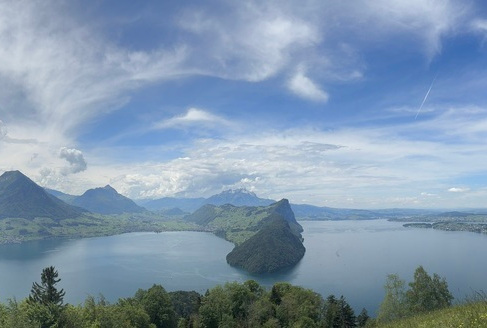
\includegraphics[width=5cm]{./chapters/introduction/scripts/denoising/natural}};
		\node [anchor=north, imagenode] at (0, -.1) {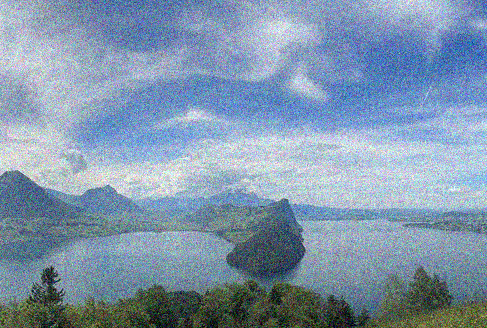
\includegraphics[width=5cm]{./chapters/introduction/scripts/denoising/noisy}};
		\node [anchor=south, imagenode] at (5.5, 0) {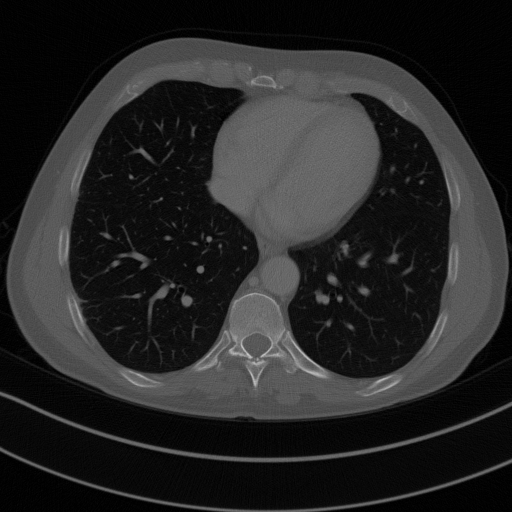
\includegraphics[width=5cm]{./chapters/introduction/scripts/ct/anatomy}};
		\node [anchor=north, imagenode] at (5.5, -.1) {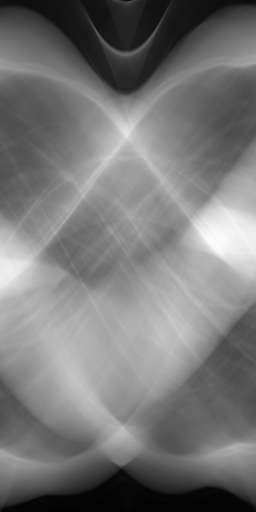
\includegraphics[rotate=90, width=5cm]{./chapters/introduction/scripts/ct/sinogram}};
		\node [anchor=south, imagenode] at (11, 0) {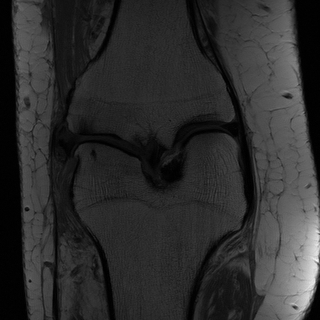
\includegraphics[rotate=180,width=5cm]{./chapters/introduction/scripts/mri/image}};
		\foreach \coil in {0,...,7}
		{
			\node [anchor=north, imagenode] at (10.5+\coil/7, -.1-\coil/7) {\includegraphics[width=2.7cm]{./chapters/introduction/scripts/mri/coil_\coil}};
		}
	\end{tikzpicture}
	\caption[Examples of inverse problems in imaging]{%
		Examples of inverse problems in imaging:
		In the top row, the first column shows a natural scene, the second column shows an axial cross section of the human thorax from an \xray{} \glsxtrshort{ct} scan, and the third column shows a coronal cross section of the human knee from an \gls{mri} scan.
		The bottom row shows the corresponding noisy observations.
	}%
	\label{fig:inverse problems examples}
\end{figure*}

The first column in \cref{fig:inverse problems examples} shows an image of a natural scene (top row) and its \emph{noisy} observation (bottom row).\footnote{%
	This is the Vierwaldstättersee in Switzerland; the image was taken by the author.
}
Each channel of each pixel in the observation is corrupted with additive Gaussian noise.
Formally, the underlying cause is a signal with square pixels that have three color channels each.
Every channel can take one a real value and we say that the signal, which we endow with its own symbol, \( \Signal \), is an element of the vector space \( \R^{\Height \times \Width \times \num{3}} \).
Then, each entry in the observation, which we endow with its own symbol, \( \Data \), is given by
\begin{equation}
	\Data_{i, j, k} = \Signal_{i, j, k} + \Noise_{i, j, k}
\end{equation}
where \( \Noise_{i, j, k} \) is normally distributed with mean zero.
More compactly,
\begin{equation}
	\Data = \Signal + \Noise,
\end{equation}
and hence the space of signal coincides with that of the observation: \( \Data \in \R^{\Height \times \Width \times \num{3}} \).
The goal of solving the inverse problem is to recover the unknown signal \( x \) from the observation \( y \).

Images of natural scenes are noisy when the sensors capture too few photons, which is common in low-light situations, when capturing fast-moving objects, or with small sensors in hand-held devices.
The denoising problem is also significant in a broader context due to its close relationship to density estimation via Tweedie's identity, discussed in~\cref{chap:pogmdm}.
In fact, denoising algorithms are currently the foundation of state-of-the-art image generation algorithms (in the form of diffusion models, see e.g.~\cite{Karras2022edm}) as well as image reconstruction algorithms (in the form of plug-and-play methods, see e.g.~\cite{Hurault2024}).

The second column in \cref{fig:inverse problems examples} shows an axial cross-section of the human thorax obtained from an \xray{} \gls{ct} scan (top row) and its observation (bottom row).
Each pixel in the signal represents the linear \xray{} attenuation coefficient of the tissue, while each entry in the observation is an \emph{area integral} of this coefficient over the cone spanned by the \xray{} source and a detector element.

In this scenario, the signal and the observation are in different spaces.
When the \xray{} camera has \( n_d \) detectors and data are acquired at \( n_a \) angles during a half-circle rotation of the source around the anatomy, the observation consists of \( n_d \times n_a \) real numbers.
Visualizing these observations in rectilinear coordinates, i.e.\ as an image \( y \in \R^{n_d \times n_a} \) yields the \emph{sinogram} shown in the bottom row.
There, the data are also noisy due to thermal noise in the measurement channels formally described by
\begin{equation}
	\Data = R\Signal + \Noise.
\end{equation}
Here, \( \map{R}{\R^{\Height \times \Width}}{\R^{n_d \times n_a}} \) is a \emph{linear} operator that models \( n_d \times n_a \) area integrals according to the measurement geometry.\footnote{%
	We chose the symbol \( R \) here to emphasize the close relation to the \emph{Radon transform}.%
}
The multiplicative Poisson noise that is typically encountered in \xray{} imaging is well approximated by heteroscedastic additive Gaussian noise \( \Noise \)~\cite{thibault_statistical_2007}.

\xray{} \gls{ct} images provide excellent hard-tissue contrast and are critical in clinical practice.
However, \xray{} radiation can have adverse health effects, making it essential to minimize radiation exposure while maintaining diagnostic value of the images.
This can be achieved by reducing the \xray{} tube current, which results in a decrease in signal-to-noise ratio.
Alternatively, SparseCT approaches~\cite{chen_sparsect_2019,Koesters2017} block the \xray{}s from entering the tissue via multi-slit collimators (effectively reducing the number of detectors) and angular undersampling approaches~\cite{Chen2008} via a shutter (effectively reducing the number of angles).
In any case, missing or noisy data makes the reconstruction problem more challenging and necessitates robust algorithms that can adapt to the measurement setup.

The third column in~\cref{fig:inverse problems examples} shows a coronal cross-section of the human knee obtained from an \gls{mri} scan (top row) and its observation (bottom row).
In \gls{mri}, the scanner's receiver coil measures the changes in the magnetism of nuclei excited by radio-frequency pulses.
By encoding different spatial frequencies via excitation coils, each entry in the observation correspond to a Fourier coefficient of the underlying signal.

Modern \gls{mri} systems often utilize multiple receiver coils to achieve faster acquisition, as pioneered by Roemer et al.~\cite{Roemer1990}.
There, the data depend on the spatially varying coil sensitivities of the receiver coils and the measurement process can be formalized as
\begin{equation}
	\begin{aligned}
		\Data_{\num{1}} &= \Mask \Fourier (\Signal \odot \CoilSensitivity_{\num{1}}) + \Noise_{\num{1}}, \\
		\Data_{\num{2}} &= \Mask \Fourier (\Signal \odot \CoilSensitivity_{\num{2}}) + \Noise_{\num{2}}, \\
				&\vdotswithin{=}\\
		\Data_\NumCoils &= \Mask \Fourier (\Signal \odot \CoilSensitivity_\NumCoils) + \Noise_\NumCoils. \\
	\end{aligned}
	\label{eq:intro mri forward}
\end{equation}
Here, \( y_{\num{1}}, y_{\num{2}}, \dotsc, y_\NumCoils \in \C^{\NumFrequencies} \) are the data from the \( \NumCoils \in \mathbb{N} \) receiver coils.
The data of the \( i \)-th coil are related to the signal \( \Signal \in \C^{\Height \times \Width} \) and the coil sensitivity \( \CoilSensitivity_i \in \C^{\Height \times \Width} \) through the two-dimensional discrete Fourier transform \( \map{F}{\C^{\Height \times \Width}}{\C^{\Height \times \Width}} \).
The coil sensitivities are usually unknown and depend on the dielectric properties of the imaged anatomy, necessitating their estimation along with the signal~\cite{Knoll2011}.
This results in a \emph{nonlinear} relationship between the data and the estimation variables.

\Gls{mri} images provide excellent soft-tissue contrast and are invaluable in clinical practice.
However, long acquisition times limit patient throughput, leading to extensive research dedicated to minimizing the acquisition time while maintaining diagnostic value of the images.
One way to reduce the acquisition time that does not necessitate changes to the hardware is to acquire less data, which is modeled by the frequency selection operator \( \map{M}{\C^{\Height \times \Width}}{\C^{\NumFrequencies}} \) in~\cref{eq:intro mri forward}.
The observation in the third column in~\cref{fig:inverse problems examples} uses a classical Cartesian frequency selection with unacquired frequencies shown in black.
It is evident that reducing available data makes retaining diagnostic value more challenging.
In addition, to account for particular anatomical features the frequency selection is subject to change in clinical practice.
This again emphasizes the need for robust and adaptable algorithms.

The discussion above suggests a general formulation of a (possibly nonlinear) inverse problem:
\begin{equation}
	\Data = \Forward(\Signal) + \Noise.
\end{equation}
Here, \( \Data \) belongs to some space \( \mathcal{Y} \), \( \Signal \) belongs to some space \( \mathcal{X} \), \( \Forward \) maps from \( \mathcal{X} \) to \( \mathcal{Y} \) encoding the measurement process, and \( \Noise \in \mathcal{Y} \) models measurement noise.
In this thesis, \( \mathcal{X} \) and \( \mathcal{Y} \) are finite-dimensional vector spaces, and we assume that \( \Forward \) is known exactly.
The next section discusses classical approaches to recover the underlying cause \( \Signal \) from an observation \( \Data \).
The limitations of classical approaches lead to the consideration of modern data-driven approaches.
\section{Variational methods and Bayes theorem}
\label{sec:variation methods and bayes theorem}
In this section, we provide a brief historical perspective on classical approaches to solving inverse problems.
This perspective is without an numerical example; in~\cref{chap:regularizers}, we discuss the benefits and drawbacks of these approaches through a prototypical \gls{mri} reconstruction problem.
We focus on classical variational methods, regularization techniques, and the accompanying probabilistic interpretation, highlighting the subtleties and the necessity for proper probabilistic modeling.

A common approach to recovering the underlying signal from observations is to minimize the discrepancy to the observation, as measured through the forward operator.
However, this problem is often ill-posed because many signals might explain the observation equally well.
Therefore, \emph{regularization} techniques have been developed.
These techniques introduce and additional \emph{regularization} term, which acts solely on the reconstruction.
Among all signals that fit the observation, the regularization term favors those with desirable properties.
For example, the property of a \emph{bounded norm} of the signal leads to the famous variational problem
\begin{equation}
	\argmin_{\Signal \in \mathcal{X}} \Half \norm{\Forward(\Signal) - \Data}^{\num{2}} + \tfrac{\lambda}{2} \norm{\Signal}^{\num{2}}.
\end{equation}
This form of regularization is usually attributed to Tikhonov~\cite{tikhonov_solution_1963} and Phillips~\cite{phillips_technique_1962}.
Here, the first term measures the squared deviation of the signal from the observation under the forward operator, and the second term ensures that the norm of the signal remains bounded.
The \emph{regularization parameter} \( \lambda > \num{0} \) controls the influence of the penalization of the norm.

In inverse problems in imaging, magnitude penalization results in dark images and is rarely useful.\footnote{%
	See the \gls{mri} example in~\cref{chap:regularizers}.
}
Instead, an extremely popular approach is to penalize the \emph{total variation} in the image.
This technique penalizes the difference between neighboring pixels absolutely, rather than the magnitude quadratically.
Introduced by Rudin, Osher, and Fatemi~\cite{rudin_nonlinear_1992} in \num{1992}, this idea has inspired extensive literature on designing regularizers~\cite{Benning_Burger_2018,bredies_total_2010,RoBl09} and optimization algorithms~\cite{chambolle_primal_2010}.

Generally, the variational approach to inverse problems amounts to solving the optimization problem
\begin{equation}
	\argmin_{\Signal \in \mathcal{X}} D(\Signal, \Data) + R(\Signal).
	\label{eq:intro variational}
\end{equation}
The objective consists of two terms:
The \emph{data fidelity term} \( \map{D}{\mathcal{X} \times \mathcal{Y}}{\R} \), which penalizes deviations of the signal from the observation by utilizing the forward operator, and the \emph{regularization term} \( \map{R}{\mathcal{X}}{\R} \), which penalizes undesired characteristics of the signal.

While the variational approach is versatile, choosing the appropriate regularizer can be challenging.
From a statistical perspective, the regularizer is related to the \emph{prior distribution} of the underlying signal in \gls{map} inference.
These concepts are treated more rigorously in~\cref{chap:preliminaries}, and a more formal treatment of inverse problems in the Bayesian perspective can be found in~\cite{Stuart_2010}.
According to Bayes theorem, the \emph{posterior density} of a signal given the data \( y \) is
\begin{equation}
	p_{X \mid Y}(\Signal, \Data) = \frac{p_{Y\mid X}(\Signal, \Data)p_X(\Signal)}{\int_{\mathcal{X}}p_{Y\mid X}(\xi, \Data)p_X(\xi)\,\mathrm{d}\xi}.
	\label{eq:intro bayes}
\end{equation}
Here, \( p_{Y\mid X} \) is the \emph{data likelihood}, which quantifies the agreement between the signal and the data.
In inverse problems in imaging, the data likelihood is typically determined by the forward model and noise statistics.
Additionally, \( p_X \) is the \emph{prior}, which quantifies the likelihood of the signal based on characteristics of reference signals.

The posterior density quantifies the likelihood of a signal given an observation \( y \).
Commonly, we aim to find the signal that best explains the observation by maximizing the posterior density:
\begin{equation}
	\argmax_{\Signal \in \mathcal{X}} p_{X \mid Y}(x, y).
	\label{eq:intro map}
\end{equation}
Equivalently, by taking the negative logarithm and observing that the denominator in~\cref{eq:intro bayes} is constant with respect to the signal, we get
\begin{equation}
	\argmin_{\Signal \in \mathcal{X}} - \log p_{Y\mid X}(\Signal, \Data) - \log p_X(\Signal).
	\label{eq:intro min neg log}
\end{equation}
Comparing \cref{eq:intro variational} and \cref{eq:intro min neg log}, we relate the data fidelity term \( D \) to the negative data log-likelihood \( - \log p_{Y \mid Z} \) and the regularization term \( R \) to the negative log-prior \( - \log p_X \).

The probabilistic interpretation is the basis of many modern data-driven approaches to inverse problems and provides a rigorous framework for other probabilistic concepts such as uncertainty quantification.
In this thesis, we adopt this interpretation and strictly separate the likelihood and prior.
Consequently, finding an effective regularizer amounts to fitting a parametric model to the prior density of reference signals.
However, this comes with subtleties that we uncover by invoking decision theory.
\section{Bayes estimators}
The equivalence between the classical variational approach to inverse problems and \gls{map} estimation is evident \enquote{algebraically} by comparing~\cref{eq:intro variational} and~\cref{eq:intro min neg log}.
However, this does not imply that a regularizer that leads to good reconstructions in~\cref{eq:intro variational} is a necessarily a good model of the true negative log-prior.
The standard metric for comparing reconstructions to the reference is the \gls{mse} (\cref{def:mse}).\footnote{equivalently, \gls{psnr} (\cref{def:psnr})}
Given data \( \Data \) and the corresponding posterior \( p_{X \mid Y}(\argm, \Data) \), finding a Bayes estimator with the \gls{mse} loss involves solving
\begin{equation}
	\argmin_{\Signal \in \mathcal{X}} \int_{\mathcal{X}} \norm{\Signal - \Signal^\prime}^{\num{2}} p_{X\mid Y}(\Signal^\prime, \Data)\,\mathrm{d}\Signal^\prime,
\end{equation}
which is known (see e.g.~\cite[page 172]{Jaynes_2003}) to be the posterior expectation
\begin{equation}
	\int_{\mathcal{X}} \Signal\,p_{X \mid Y}(\Signal, \Data)\,\mathrm{d}\Signal.
\end{equation}
In contrast, the variational formulation seeks the \gls{map} estimate.
Thus, there is a mismatch between the evaluation metric and the inference procedure:
a regularizer that leads to a small \gls{mse} via \gls{map} inference is not necessarily a good model of the negative log-prior.
Conversely, a good model of the negative log-prior does not necessarily lead to small \gls{mse} via \gls{map} inference.

Generally, although the variational approach \emph{can} be interpreted probabilistically, the regularizer does not have to be derived from statistics of reference data.
Often, a regularizer can be useful for downstream tasks without any specific relation to reference statistics.
In such cases, estimators of the form~\cref{eq:intro variational} are sometimes referred to as \emph{maximum penalized likelihood estimators}~\cite{bohra_phdthesis,gribonval_penalized_2011}.
In addition, Gribonval~\cite{gribonval_penalized_2011} has pointed out that for some class of regularizers, solutions to~\cref{eq:intro variational} are \gls{mmse} estimates with respect to \emph{some} prior.
However, in general the regularizer is not the negative log of this prior.

In summary, when pursuing strict separation of likelihood and prior and adopting the \emph{natural} probabilistic interpretation of the regularizer, evaluation (with the standard metrics) should be done on the \gls{mmse} estimate.
We follow this principle throughout this thesis:
In~\cref{chap:deep neural regularizers}, we learn a deep neural regularizer and compute \gls{mmse} estimates by sampling the posterior with \gls{mcmc} methods.
In~\cref{chap:pogmdm}, the principled construction of the regularizer allows us to compute \gls{mmse} estimates for denoising problems with one gradient evaluation.

\section{Data-driven regularizers}
When adopting the probabilistic interpretation, finding a good regularizer amounts to learning the reference density.
In the context of inverse problems in imaging, this was pursued in the foundational works by Zhu and Mumford in their series of papers~\cite{zhu_prior_1997,zhu_minimax_1997,zhu_filters_1998} that lead to the celebrated \gls{frame} model.
However, their approach relied on hand-selected filters and is problematic in the context of gradient-based optimization due to the use of piecewise constant functions.
Welling, Hinton, and Osindero~\cite{welling_learning_2002} proposed learning the distribution of image patches via a product of one-dimensional experts, where the experts act on filter responses, and both the filters and the parameters of the experts\footnote{they chose Student-t experts} are learned.
However, their learning algorithm does not scale to large images.
The \gls{foe} model by Roth and Black~\cite{RoBl09} extends this model to large images by replacing the Gibbs sampler relying on matrix inversions with a gradient-based \gls{mcmc} sampling algorithm.
Crucially, they obtain a \emph{translation invariant} prior by sharing the same filters and experts across \emph{all} patches in the image.

The \gls{foe} approach shares a lot of similarities with the learned regularizers we discuss in this thesis.
In particular, the learning setup of the deep neural regularizer we propose in~\cref{chap:deep neural regularizers} is largely the same;
there we also resort to a gradient-based \gls{mcmc} sampling algorithm to fit an intractable model to the reference density.
However, instead of the product-of-experts structure, we design an expressive deep neural regularizer that is explicitly \emph{not} translation invariant, to model the statistics of \gls{mri} scans of the human knee.
In contrast, in~\cref{chap:pogmdm} we revisit the translation invariant \gls{foe} structure but use more efficient learning algorithms based on score matching~\cite{hyvarinen_estimation_2005} and additionally incorporate ideas from diffusion models~\cite{song_scorebased_2021}.

\section{Contributions and outline}
In recent years, data-driven methods have become state-of-the-art in many inverse problems in imaging.
The survey paper~\cite{Arridge_Maass_Öktem_Schönlieb_2019} of Arridge, Maass, Öktem, and Schönlieb provides a comprehensive overview of recent advances.
This can largely be attributed to the availability of large datasets, the increase in parallel processing power of graphics processing units, and the development and free availability of automatic differentiation frameworks such as PyTorch~\cite{paszke_pytorch_2019}.
Concurrently, there has been a shift towards \emph{discriminative} signal recovery approaches, where the separation between data likelihood and prior is largely lost, making the models harder to interpret.
The difference between \emph{generative} and \emph{discriminative} signal recovery approaches is discussed in detail in~\cref{chap:machine-learning}.
In the context of inverse problems in imaging, likelihoods are frequently subject to change, making discriminative point estimators problematic---an issue illustrated with an example in \cref{fig:unet kspace ablation}.

In this thesis, we aim to leverage modern data-driven approaches within the framework of classical variational approaches to inverse problems.
In particular, in light of the discussion in~\cref{sec:variation methods and bayes theorem}, finding a good regularizer amounts to fitting a parametric model to the prior density of reference signals---\emph{generative modeling}.
For inverse problems in \gls{mri}, we design a deep neural regularizer that models the negative log-prior distribution of \gls{mri} images of human knees.
We demonstrate that the learned model encodes high-level statistics by synthesizing realistic-looking images \emph{without data}.
We use the learned regularizer alongside a fast algorithm for solving the \emph{nonlinear} inversion problem encountered in parallel \gls{mri} and achieve state-of-the-art reconstruction results.
For inverse problems with natural images, we revisit classical translation-invariant priors and propose replacing computationally intensive maximum likelihood training with denoising score matching.
By adopting ideas from diffusion models and carefully selecting filters and parametrization of the experts, we develop a model that serves as an \gls{mse}-optimal denoiser for Gaussian noise with arbitrary variance.

This thesis is intended to be largely self-contained.
To this end,~\cref{chap:preliminaries} provides mathematical preliminaries of functional analysis, probability theory, stochastic differential equations, optimization, and the representation of digital images.
These preliminaries are covered with (possibly excessive) rigor.
Familiar readers can skip this chapter entirely, although forward references are provided to where the concepts are used in the remainder of the thesis.
In \cref{chap:machine-learning}, we review basic concepts from machine learning and neural networks.
In particular, the chapter introduces the neural network terminology used throughout this thesis and emphasizes the difference between generative and discriminative learning.
\Cref{chap:regularizers} provides a historical overview of the development of regularizers in imaging, using \gls{mri} reconstruction as a running example.
There, we also superficially introduce our proposed models and compare their performance to classical regularizers.

The previous chapters serve as an introduction to our contributions, which are discussed in~\cref{chap:deep neural regularizers} and~\cref{chap:pogmdm}.
In particular, in~\cref{chap:deep neural regularizers} we design a deep neural regularizer for \gls{mri} reconstruction, exploiting the characteristics of images in the application domain.
Due to the alignment of the patient in the scanner, features in the images consistently appear in distinct locations, and the anatomy exhibits subtle non-local dependencies that our regularizer can capture.
In this chapter, we also revisit joint nonlinear inversion for parallel \gls{mri} reconstruction and propose a fast algorithm that eliminates the need for calibration scans for coil sensitivity estimation.
In~\cref{chap:pogmdm} we revisit the structure of classical translation invariant regularizers and show how to efficiently learn a \gls{foe} type model with score matching.
By leveraging ideas from diffusion models we retrieve a model that can act as an \gls{mse} optimal denoiser for Gaussian noise with arbitrary variance.
Finally, we conclude the thesis and suggest future research directions in~\cref{chap:conclusion}.

\chapter{Preliminaries}%
\label{chap:preliminaries}%
\graphicspath{{./chapters/preliminaries/scripts/}}%
In\marginnote{\footnotesize \textbf{Contents:}\\\localtableofcontents} this chapter, we recall important mathematical concepts that are used in the remainder of this thesis.
In particular, we recall standard results from functional analysis, probability theory, stochastic differential equations, and optimization and define our notion of images as signals defined on a finite Cartesian grid.
This chapter serves primarily as a reference, with no new contributions.
Subsequent chapters will refer back to the definitions, theorems, and algorithms discussed here as needed.
However, \cref{sec:pdes} on stochastic differential equations and \cref{sec:optimization} on optimization discuss some peculiarities of how the concepts are used in this thesis.
\section{Functional analysis}
In this section, we recall definitions and results from analysis, topology, and measure theory used in the subsequent sections.
This overview is adapted from~\cite{Alt2016,beck_firstorder_2017,Klenke2014}.
In this thesis, the field \( \Field \) are either the real numbers \( \R \) or the complex numbers \( \C \).
For any \( x \in \Field \), we denote the absolute value by
\begin{equation}
	\abs{x} \coloneqq \sqrt{x\conj{x}}\ \text{with}\ \conj{x} = \begin{cases}
		\mathfrak{Re}(x) - \mathfrak{Im}(x) &\ \text{if}\ \Field = \C, \\
		x &\ \text{if}\ \Field = \R.
	\end{cases}
\end{equation}
\subsection{Vector spaces}
\begin{definition}[Vector space]%
	\label{def:vector space}
	A \emph{vector space} over a field \( \Field \) is a nonempty set \( \V \) endowed with a binary function \( \map{(\argm +_{\V} \argm)}{\V \times \V}{\V} \) (\enquote{vector addition}) and a binary function \( \map{(\argm \cdot_{\V} \argm)}{\Field \times \V}{\V} \) (\enquote{scalar multiplication}) such that the following holds:
	\begin{enumerate}
		\item Let \( x \), \( y \), and \( z \) be arbitrary elements of \( \V \). The vector addition satisfies
		\begin{enumerate}
			\item \( x +_{\V} (y +_{\V} z) = (x +_{\V} y) +_{\V} z. \)
			\item \( x +_{\V} y = y +_{\V} x. \)
			\item There exists a unique element \( \num{0}_{\V} \in \V \) such that \( x +_{\V} \num{0}_{\V} = x \).
			\item There exists an element \( -x \in \V \) such that \( x +_{\V} (-x) = \num{0} \).
		\end{enumerate}
		\item Let \( a \) and \( b \) be arbitrary elements of the field \( \Field \) and let \( x \) be an arbitrary element of \( \V \). The scalar multiplication satisfies
		\begin{enumerate}
			\item \( a\cdot_{\V}(b\cdot_{\V}x) = (a\cdot_{\V}b)\cdot_{\V}x \).
			\item Let \( \num{1}_{\Field} \) denote the multiplicative identity in \( \Field \). Then \( \num{1}_{\Field}\cdot_{\V}x = x \).
		\end{enumerate}
		\item The scalar multiplication distributes with respect to vector addition and field addition:
		\begin{enumerate}
			\item \( a\cdot_{\V}(x +_{\V} y) = a\cdot_{\V}x +_{\V} a\cdot_{\V}y \).
			\item \( (a +_{\Field} b)\cdot_{\V}x = a\cdot_{\V}x +_{\V} b\cdot_{\V}x \).
		\end{enumerate}
	\end{enumerate}
\end{definition}

The most prominent example of a vector space is \( \R^n \).
Its base field are the real numbers \( \R \), the set \( \V \) are all \( n \)-tuples with real components and vector addition and scalar multiplication are defined as
\begin{equation}
	\begin{pmatrix}
		x_{\num{1}} \\ x_{\num{2}} \\ \vdots \\ x_n
		\end{pmatrix} +_{\R^n} \begin{pmatrix}
		y_{\num{1}} \\ y_{\num{2}} \\ \vdots \\ y_n
	\end{pmatrix} = \begin{pmatrix}
	x_{\num{1}} +_{\R} y_{\num{1}} \\ x_{\num{2}} +_{\R} y_{\num{2}} \\ \vdots \\ x_n +_{\R} y_n
	\end{pmatrix},\quad a\cdot_{\R^n} \begin{pmatrix}
	x_{\num{1}} \\ x_{\num{2}} \\ \vdots \\ x_n
	\end{pmatrix} = \begin{pmatrix}
	a\cdot_{\R}x_{\num{1}} \\ a\cdot_{\R}x_{\num{2}} \\ \vdots \\ a\cdot_{\R}x_n
	\end{pmatrix}.
\end{equation}
Here \( x = (x_{\num{1}}, x_{\num{2}}, \dotsc, x_n)\tp \), \( y = (y_{\num{1}}, y_{\num{2}}, \dotsc, y_n)\tp \in \R^n \) and \( a \in \R \).
In this thesis, it is not necessary to distinguish between the set of a vector space and the vector space itself (the (set, addition, multiplication) triple).
In other words, \( \R^n \) refers to the \emph{vector space} and implicitly carries over the operations as defined above.

\subsection{Inner products}
It is well known that two vectors in \( \R^n \) are \emph{orthogonal}, if their \emph{dot product} is zero.
As a generalization of the dot product, inner products can be used to impose geometry onto a vector space by mapping a pair of vectors to a scalar in the underlying field.
\begin{definition}[Inner product]%
	\label{def:inner product}
	Let \( \V \) be a vector space over a field \( \Field \).
	An \emph{inner product} \( \map{\inprod{\argm}{\argm}_{\V}}{\V \times \V}{\Field} \) satisfies
	\begin{enumerate}
		\item \( \inprod{x}{y}_{\V} = \conj{\inprod{y}{x}_{\V}} \) for any \( x , y \) in \( \V \).
		\item \( \inprod{a_{\num{1}} x_{\num{1}} + a_{\num{2}} x_{\num{2}}}{y}_{\V} = a_{\num{1}}\inprod{x_{\num{1}}}{y}_{\V} + a_{\num{2}}\inprod{x_{\num{2}}}{y}_{\V} \) for any \( a_{\num{1}}, a_{\num{2}} \in \Field \) and any \( x, y \in \V \).
		\item \( \inprod{x}{x}_{\V} \geq \num{0} \) for any \( x \in \V \) and \( \inprod{x}{x}_{\V} \) if and only if \( x = \num{0}_{\V} \).
	\end{enumerate}
\end{definition}
We call the ordered pair \( (\V, \inprod{\argm}{\argm}_{\V}) \) an \emph{inner product space}.
The aforementioned dot product on \( \R^n \) is the map
\begin{equation}
	\inprod{x}{y}_{\R^n} = \sum_{i={\num{1}}}^n x_i y_i.
\end{equation}
\subsection{Norms}
We use norms to rigorously define notions of distance from the origin in a vector space.
In particular, any sensible distance function should absolutely commute with scaling, obey the triangle inequality, and assign zero only to the zero vector.
This motivates the following definition:
\begin{definition}[Norm]%
	\label{def:norm}
	Let \( \V \) be a vector space over a field \( \Field \).
	A norm \( \map{\norm{}_{\V}}{\V}{\R} \) satisfies
	\begin{enumerate}
		\item \( \norm{ax}_{\V} = \abs{a}\,\norm{x}_{\V} \) for any \( x \in \V \) and \( a \in \Field \).\label{def:norm item one}
		\item \( \norm{x + y}_{\V} \leq \norm{x}_{\V} + \norm{y}_{\V} \) for all \( x, y \in \V \).\label{def:norm item two}
		\item \( \norm{x}_{\V} = \num{0} \implies x = \num{0}_{\V} \).
	\end{enumerate}
\end{definition}
Note that~\cref{def:norm item one} implies \( \norm{\num{0}_{\V}}_{\V} = \num{0} \) and that~\cref{def:norm item one} and~\cref{def:norm item two} imply nonnegativity: \( \norm{x}_{\V} \geq \num{0} \), another sensible property of a distance function.

A function that satisfies~\cref{def:norm item one} and~\cref{def:norm item two} but maps some nonzero vectors to zero is called a \emph{seminorm}.
The ordered pair \( (\V, \norm{}_{\V}) \) is called a \emph{normed vector space}.
Any inner product on a vector space \( \V \) induces a norm through \( \norm{}_{\V} = \sqrt{\inprod{\argm}{\argm}}_{\V} \).

In the previous definitions, we endowed the operations of vector addition, scalar multiplication, inner product, and norms with a subscript to emphasize the vector space these operations occur in.
However, this notation is overly verbose and usually the space is evident from the context.
Thus, in the remainder of this thesis we omit this subscript unless needed.

An important family of norms are the \( \ell^p \) norms on \( \Field^n \) defined as
\begin{equation}
	\norm{x}_{p} \coloneqq \begin{cases}
		\displaystyle\biggl( \sum_{i=\num{1}}^n \abs{x_i}^p\biggr)^{\frac{1}{p}} &\ \text{if}\ \num{1} \leq p < \infty, \\
		\displaystyle\max_{i=\num{1},\dotsc,n} \abs{x_i} &\ \text{if}\ p = \infty.
	\end{cases}
\end{equation}
\begin{sidefigure}
	\begin{tikzpicture}
		\begin{axis}[
			legend image with text/.style={%
				legend image code/.code={%
					\node[anchor=center] at (0cm,0cm) {#1};
				}
			},
			legend columns=-1,
			legend image code/.code={%
				\draw[mark repeat=2,mark phase=2,#1] 
					plot coordinates {
						(0cm,0cm) 
						(0.2cm,0cm)
						(0.4cm,0cm)
					};
			},
			legend style={%
				font=\fontsize{7pt}{8pt}\selectfont,
				at={(0.0, 1.05)},
				anchor=west,
				draw=none
			},
			trig format plots=rad,
			axis equal,
			width=4cm,
			scale only axis,
			marginplot,
			xmin=-1.2, xmax=1.2,
			ymin=-1.2, ymax=1.2,
			axis on top,
			thick,
		]
			\addlegendimage{legend image with text={}}
			\addlegendentry{$p=$}
			\addplot+ coordinates {(0, 1) (-1, 0) (0, -1) (1, 0) (0, 1)};
			\addlegendentry{$1$}
			\addplot+ [domain=0:2*pi, samples=200] ({sin(x)}, {cos(x)});
			\addlegendentry{$2$}
			\addplot+ [raw gnuplot] gnuplot {%
				set isosamples 500;
				set contour base;
				set cntrparam levels discrete 1.0;
				unset surface;
				set xrange [-1.1:1.1];
				set yrange [-1.1:1.1];
				splot (abs(x)**5+abs(y)**5)**(1./5.);
			};
			\addlegendentry{$5$}
			\addplot+ coordinates {(1,1) (-1,1) (-1,-1) (1,-1) (1,1)};
			\addlegendentry{$\infty$}
		\end{axis}
	\end{tikzpicture}
	\caption[Unit spheres of \( p \)-norms]{%
		Unit spheres of different \( p \)-norms in \( \R^{\num{2}} \).
	}%
	\label{fig:norm balls}
\end{sidefigure}
\Cref{fig:norm balls} visualizes the unit spheres of different \( \ell^p \) norms in \( \R^{\num{2}} \):
The unit-one-norm-sphere is a rhombus, the unit-two-norm-sphere is a circle and as \( p \) approaches infinity, the unit-\( p \)-norm-sphere approaches a square.
\subsection{Topology}
In this section, we recall topological concepts that are required for understanding the optimization algorithms used in this thesis.
To proceed, we first define norm balls:
Let \( (\V, \norm{}) \) be a normed vector space.
We denote with
\begin{equation}
	\Ball{\norm{}}{c}{r} \coloneqq \Set{x \in \V \given \norm{x - c} < r}
\end{equation}
the open norm ball with respect to the norm \( \norm{} \) and radius \( r > \num{0} \), centered around \( x \in \V \).

A set \( S \subseteq \V \) is
\begin{itemize}
	\item \emph{bounded} if there exists a radius \( r > \num{0} \) such that \( S \subset \Ball{\norm{}}{\num{0}_{\V}}{r} \).
	\item \emph{open} if for all \( x \in S \) there exists an \( \epsilon > \num{0} \) such that \( \Ball{\norm{}}{x}{\epsilon} \subset S \).
	\item \emph{closed} if \( \V \setminus S \) is open.
	\item \emph{compact} if every open cover of \( S \) has a finite subcover.
\end{itemize}
The last definition is somewhat technical and overkill for our purposes --- thus we recall the simpler definition of compactness in the Euclidean case:
\begin{theorem}[Heine-Borel Theorem]%
	\label{def:heine-borel}
	Let \( S \subset \Field^n \).
	Then, the following statements are equivalent:
	\begin{itemize}
		\item \( S \) is bounded and closed.
		\item Every open cover of \( S \) has a finite subcover.
	\end{itemize}
\end{theorem}
Other basic notions that we will need for the rest of this section are the interior and the closure of a set:
\begin{definition}[Interior, closure, boundary]%
	\label{def:interior closure boundary}
	Let \( (\V, \norm{}) \) be a normed vector space and let \( S \subseteq \V \).
	\begin{itemize}
		\item A point \( x \in S \) is an \emph{interior point} of \( S \) if there exists an open set \( O \subseteq S \) such that \( x \in O \).
			The set of all interior points forms the \emph{interior} of \( S \), denoted by \( \Interior{S} \).
		\item A point \( x \in \V \) is a \emph{point of closure} of \( S \) if for every open set \( O \subseteq S \) that contains \( x \) there exists an \( s \in S \) such that \( s \in O \).
			The set of all points of closure of \( S \) is the \emph{closure} of \( S \), denoted by \( \Closure{S} \).
		\item The \emph{boundary} of \( S \) is the set \( \Boundary{S} \coloneqq \Closure{S} \setminus \Interior{S} \).
	\end{itemize}
\end{definition}
Finally, we define the neighborhood of a point in a normed space:
\begin{definition}[Neighborhood]%
	\label{def:neighborhood}
	Let \( (\V, \norm{}) \) be a normed vector space.
	A set \( \ASet \) is a \emph{neighborhood} of a point \( x \in \V \) if there exists a radius \( r > \num{0} \) such that \( \Ball{\norm{}}{x}{r} \) is contained in \( \ASet \).
\end{definition}
\subsection{Convergence, completeness, and continuity}
In this section, we introduce the concepts of convergence of sequences, which relates to completeness of spaces and finally continuity of functions.
In this journey, we also rigorously define Hilbert spaces.
To start, let \( (\V, \norm{}) \) be a normed vector space.
We call a map from the natural numbers to \( \V \) a \emph{sequence} and use the shorthand notation \( x^n \coloneqq x(n) \) for a sequence \( x \).
\begin{definition}[Limit and convergence of a sequence]%
	\label{def:limit and convergence of a sequence}
	A point \( x_{\num{0}} \in \V \) is the \emph{limit} of a sequence \( x \) if for all \( \epsilon > \num{0} \) there exists and \( N \in \mathbb{N} \) such that for every \( n \geq N \), \( \norm{x^n - x_{\num{0}}} < \epsilon \).
	If such a point exists, we say that \( x \) \emph{converges} to \( x_{\num{0}} \) and write \( x^n \to x_{\num{0}} \) as \( n \to \infty \) or
	\[
		\lim_{n\to\infty} x^n = x_{\num{0}}.
	\]
\end{definition}
To define the completeness of a space, we require the slightly relaxed notion of a Cauchy sequence:
\begin{definition}[Cauchy sequence]%
	\label{def:cauchy sequence}
	A sequence \( x \) is \emph{Cauchy} if for every \( \epsilon > \num{0} \) there exists an \( N \in \mathbb{N} \) such that for all \( i, j > N \)
	\[
		\norm{x^i - x^j} < \epsilon.
	\]
\end{definition}
In words, a sequence is Cauchy if the distance between iterates becomes arbitrarily small for large enough arguments.
However, a Cauchy sequence is not necessarily convergent---we will show some examples later.
Finally, we can characterize complete spaces:
\begin{definition}[Completeness]%
	\label{def:completeness}
	The normed vector space \( (\V, \norm{}) \) is \emph{complete} if every Cauchy sequence converges to an element of \( \V \).
	A \emph{Hilbert space} is an inner product space which is complete with respect to the induced norm \( \norm{} = \sqrt{\inprod{x}{x}} \).
	A \emph{Banach space} is a normed space that is complete w.r.t.\ its norm.
\end{definition}
Spaces that are not complete are easy to construct.
A famous example are the rational numbers endowed with the absolute value, \( (\mathbb{Q}, \abs{\argm}) \):
The sequence of rationals \( n \mapsto \bigl( \num{1} + n^{\num{-1}} \bigr)^n \) is Cauchy but does not converge in \( (\mathbb{Q}, \abs{\argm}) \).
In \( (\R, \abs{\argm}) \), it famously converges to Euler's constant.
The next theorem relates continuity of a function with the convergence of the image a sequence under the function.
To state it, we first define continuity.
For the following, we let \( (\V, \norm{}_{\V}) \) and \( (\mathbb{W}, \norm{}_{\mathbb{W}}) \) be two normed vector spaces.
\begin{definition}[Continuity]%
	\label{def:continuity}
	A function \( \map{f}{\V}{\mathbb{W}} \) is \emph{continuous at \( x_{\num{0}} \in \V \)} if for all \( \epsilon > \num{0} \) there exists a \( \delta > \num{0} \) such that \( \norm{x - x_{\num{0}}}_{\V} < \delta \) implies that \( \norm{f(x) - f(x_{\num{0}})}_{\mathbb{W}} < \epsilon \).
\end{definition}
Let \( S \subseteq V \).
We call \( f \) \emph{continuous on \( S \)} if it is continuous at every point in \( S \).
We call \( f \) \emph{continuous} if it continuous on \( \V \).
\begin{theorem}
	Let \( \map{f}{\V}{\mathbb{W}} \).
	The following statements are equivalent:
	\begin{itemize}
		\item \( f \) is continuous.
		\item For every set \( S \subseteq \mathbb{W} \) open in \( \mathbb{W} \), the preimage of \( S \) under \( f \) is open in \( \V \).
		\item For every \( x_{\num{0}} \in \V \) and every sequence \( x \) on \( \V \) such that \( x^n \to x_{\num{0}} \) in \( \V \) the sequence \( f(x^n) \to f(x_{\num{0}}) \) in \( \mathbb{W} \) as \( n \to \infty \).
	\end{itemize}
\end{theorem}
\begin{proof}
	See~\cite[section 2.17]{Alt2016}.
\end{proof}

The optimization algorithms we use in this thesis often have slightly stronger assumptions on functions.
In particular, they often require that the distance of the images of two points can be upper bounded by their distance, up to a multiplicative constant.
This is captured in the notion of Lipschitz continuity:
\begin{definition}[Lipschitz continuity]%
	\label{def:lipschitz continuity}
	A function \( \map{f}{\V}{\mathbb{W}} \) is called \emph{Lipschitz continuous} with \emph{Lipschitz constant} \( L > \num{0} \) if for all \( x, y \in \V \)
	\[
		\norm{f(x) - f(y)}_{\mathbb{W}} \leq L \norm{x - y}_{\V}.
	\]
\end{definition}
Lipschitz continuity is illustrated for a map from \( \R \) to \( \R \) in~\cref{fig:lipschitz continuity}.
\begin{sidefigure}
	\centering
	\begin{tikzpicture}% TODO: fix this with clip false... I don't like it
		\begin{axis}[marginplot, width=.95\marginparwidth,ymin=-1, ymax=1]
			\addplot [thick, maincolor, domain=-3:3] {0.9*tanh(x - 1)};
			\addplot [domain=0:2] {x - 1};
			\addplot [domain=0:2] {-x + 1};
			\fill [opacity=.2, maincolor] (1, 0) -- (0, 1) -- (-3, 1.2) -- (-3, -1.2) -- (0, -1) -- cycle;
			\fill [opacity=.2, maincolor] (1, 0) -- (2, 1) -- (3, 1.20666) -- (3, -1.20666) -- (2, -1) -- cycle;
		\end{axis}
	\end{tikzpicture}
	\caption[Geometric interpretation of Lipschitz continuity]{Geometric interpretation of Lipschitz continuity for a function over \( \R \).}%
	\label{fig:lipschitz continuity}
\end{sidefigure}
There, the dark green function always stays outside of the double cone spanned by the two black lines.
Classical examples of functions which are not Lipschitz continuous are the exponential function and the quadratic \( x \mapsto x^{\num{2}} \) over \( \R \), and \( \sqrt{\argm} \) over \( \R_+ \).
The former two examples become infinitely steep as their arguments explode, the latter becomes infinitely steep as its argument approaches zero as illustrated in~\cref{fig:sqrt not lipschitz}.
\begin{sidefigure}
	\begin{tikzpicture}[spy using outlines={rectangle, magnification=2, size=2cm, connect spies}]
		\begin{axis}[marginplot, width=.85\marginparwidth,yticklabels={}]
			\addplot [thick, maincolor, domain=0:1, samples=201] {sqrt(x)};
			\addplot [domain=0:.2] {5*x};
			\coordinate (on) at (0.07, 0.11);
			\coordinate (at) at (0.66, 0.3);
		\end{axis}
		\spy [black, overlay] on (on) in node at (at);
	\end{tikzpicture}
	\caption[\( \sqrt{\argm} \) over \( \interval{\num{0}}{\num{1}} \) is not Lipschitz continuous]{%
		\( \sqrt{\argm} \) over \( \interval{\num{0}}{\num{1}} \) is not Lipschitz continuous.
	}%
	\label{fig:sqrt not lipschitz}
\end{sidefigure}
These examples demonstrate that Lipschitz continuity is rather strong;
often it suffices that a function satisfies Lipschitz continuity \emph{locally}:
\begin{definition}[Local Lipschitz continuity]%
	\label{def:local lipschitz continuity}
	A function \( \map{f}{\V}{\mathbb{W}} \) is \emph{locally Lipschitz continuous} if for all \( x \in \V \) there exists a neighborhood (\cref{def:neighborhood}) \( N(x) \) such that the restriction of \( f \) to \( N(x) \) is Lipschitz continuous.
\end{definition}
\subsection{Measure theory}
In this section we briefly introduce concepts from measure theory.
It is mostly based on~\cite{bredies_mathematical_2018} and is by no means a complete overview of the field---its purpose is to introduce Lebesgue spaces and lay the foundations for probability theory.

Throughout the following discussion, we denote with \( \ASet \) an arbitrary non-empty set.
We denote with \( \PowerSet{\ASet} \coloneqq \Set*{\mathcal{A} \given \mathcal{A} \subseteq \ASet} \) the power set of \( \ASet \).
First, we classify sets according to closedness properties.
\begin{definition}[Closedness properties]
	Let \( \SigmaAlgebraSymbol \subseteq \PowerSet{\ASet}\) be a set of subsets, let \( \mathcal{A}, \mathcal{A}_i, \mathcal{B} \), \( i \in \mathbb{N} \) be arbitrary elements of \( \SigmaAlgebraSymbol \), and let \( \mathcal{I} \subseteq \mathbb{N} \) be a finite or infinite subset of the natural numbers.
	The set of sets \( \SigmaAlgebraSymbol \) is
	\begin{itemize}
		\item \emph{closed under intersections} if \( \mathcal{A} \cap \mathcal{B} \in \SigmaAlgebraSymbol \).
		\item \emph{closed under countable intersections} if \( \bigcap_{i \in \mathcal{I}}\mathcal{A}_i \in \SigmaAlgebraSymbol \).
		\item \emph{closed under unions} if \( \mathcal{A} \cup \mathcal{B} \in \SigmaAlgebraSymbol \).
		\item \emph{closed under countable unions} if \( \bigcup_{i \in \mathcal{I}}\mathcal{A}_i \in \SigmaAlgebraSymbol \).
		\item \emph{closed under differences} if \( \mathcal{A} \setminus \mathcal{B} \in \SigmaAlgebraSymbol \).
		\item \emph{closed under complements} if \( \mathcal{S} \setminus \mathcal{A} \in \SigmaAlgebraSymbol \).
	\end{itemize}
\end{definition}

The subsequent discussion of probability theory heavily relies on \SigmaAlgebras, which we now define and \emph{measurable spaces}, which we now define.
\begin{definition}[\SigmaAlgebra]%
	\label{def:sigma algebra}
	A set of subsets \( \SigmaAlgebraSymbol \subseteq \PowerSet{\ASet} \) is a \emph{\SigmaAlgebra{} on \( \ASet \)} if
	\begin{itemize}
		\item \( \ASet \in \SigmaAlgebraSymbol \).
		\item \( \SigmaAlgebraSymbol \) is closed under complements.
		\item \( \SigmaAlgebraSymbol \) is closed under countable unions.
	\end{itemize}
\end{definition}
\begin{definition}[Measurable space and measurable sets]%
	\label{def:measurable spaces and measureable sets}
	A pair \( (\ASet, \SigmaAlgebraSymbol) \), where \( \ASet \) is an arbitrary nonempty set and \( \SigmaAlgebraSymbol \) is a \SigmaAlgebra{} over \( \ASet \), is a \emph{measurable space}.
	The sets in \( \SigmaAlgebraSymbol \) are called \emph{measurable}.
\end{definition}
The smallest \SigmaAlgebra{} that contains a set of subsets \( \mathfrak{E} \) is called the \SigmaAlgebra{} \emph{induced} (or \emph{generated}) by \( \mathfrak{E} \), and we write \( \sigma(\mathfrak{E}) \).
For a normed vector space \( (\V, \norm{}) \) the \SigmaAlgebra{} generated by all open sets is the \emph{Borel \SigmaAlgebra} \( \BorelSigma{\ASet} \) on \( \ASet \) and its elements are \emph{Borel measurable}.

Later, we will need the notion of \SigmaAlgebras{} that are generated by (possibly more than) one map.
\begin{definition}[Generated \SigmaAlgebra~{\cite[Definition 1.79]{Klenke2014}}]%
	\label{def:generated sigma algebra}
	Let \( \ASet \) be a nonempty set and let \( I \) be an arbitrary index set.
	For any \( i \in I \) let \( (\ASet_i, \SigmaAlgebraSymbol_i) \) be a measurable space and let \( \map{X_i}{\ASet}{\ASet_i} \) be an arbitrary map.
	Then
	\begin{equation}
		\sigma(X_i, i \in I) \coloneqq \sigma\biggl( \bigcup_{i \in I} \sigma(X_i) \biggr) \coloneqq \sigma\biggl( \bigcup_{i\in I} \PreImage{X_i}(\ASet_i) \biggr)
	\end{equation}
	is the \SigmaAlgebra{} on \( \ASet \) that is \emph{generated} by \( (X_i, i \in I) \).
	This is the smallest \SigmaAlgebra{} with respect to which all \( X_i \) are measurable.
\end{definition}

Now we develop \emph{measures} to meaningfully quantify the \enquote{size} of sets.
First, we recall properties of functions on sets and then define the notion of a \emph{measure}.
\begin{definition}[Properties of functions on sets]%
	\label{def:properties of functions on sets}
	Let \( \SigmaAlgebraSymbol \subseteq \PowerSet{\ASet} \) and let \( \map{\Measure}{\SigmaAlgebraSymbol}{\interval{\num{0}}{\infty}} \) be a function on sets.
	\( \Measure \) is
	\begin{itemize}
		\item \emph{monotone} if \( \Measure(\mathcal{A}) \leq \Measure(\mathcal{B}) \) for any \( \mathcal{A}, \mathcal{B} \in \SigmaAlgebraSymbol \) such that \( \mathcal{A} \subseteq \mathcal{B} \).
		\item \emph{additive} if \( \Measure\bigl(\bigcup_{i=\num{1}}^n \mathcal{A}_i \bigr) = \sum_{i=1}^n \Measure(\mathcal{A}_i) \) for any mutually disjoint \( \mathcal{A}_{\num{1}},\mathcal{A}_{\num{2}},\allowbreak\dotsc,\allowbreak\mathcal{A}_n \in \SigmaAlgebraSymbol \) such that \( \bigcup_{i=\num{1}}^n \mathcal{A}_i \in \SigmaAlgebraSymbol \).
		\item \emph{\(\sigma\)-additive} if \( \Measure\bigl(\bigcup_{i\in\mathbb{N}} \mathcal{A}_i \bigr) = \sum_{i\in\mathbb{N}} \Measure(\mathcal{A}_i) \) for any mutually disjoint \( \mathcal{A}_{\num{1}},\allowbreak\mathcal{A}_{\num{2}},\allowbreak\dotsc \in \SigmaAlgebraSymbol \) such that \( \bigcup_{i\in \mathbb{N}} \mathcal{A}_i \in \SigmaAlgebraSymbol \).
		\item \emph{subadditive} if \( \Measure\bigl(\bigcup_{i=1}^n \mathcal{A}_i \bigr) \leq \sum_{i=\num{1}}^n \Measure(\mathcal{A}_i) \) for any \( \mathcal{A}_{1},\mathcal{A}_{\num{2}},\dotsc,\mathcal{A}_n \in \SigmaAlgebraSymbol \) such that \( \bigcup_{i=1}^n \mathcal{A}_i \in \SigmaAlgebraSymbol \).
		\item \emph{\(\sigma\)-subadditive} if \( \Measure\bigl(\bigcup_{i=1}^n \mathcal{A}_i \bigr) \leq \sum_{i\in\mathbb{N}} \Measure(\mathcal{A}_i) \) for any \( \mathcal{A}_{1},\mathcal{A}_{\num{2}},\dotsc \in \SigmaAlgebraSymbol \) such that \( \bigcup_{i\in\mathbb{N}} \mathcal{A}_i \in \SigmaAlgebraSymbol \).
	\end{itemize}
\end{definition}
\begin{definition}[Measure]%
	\label{def:measure}
	Let \( (\ASet, \SigmaAlgebraSymbol) \) be a measurable space.
	A function \( \map{\Measure}{\SigmaAlgebraSymbol}{\interval{\num{0}}{\infty}} \) is a \emph{measure} on \( (\ASet, \SigmaAlgebraSymbol) \) if
	\begin{itemize}
		\item \( \Measure(\emptyset) = \num{0} \) and
		\item \( \Measure \) is subadditive.
	\end{itemize}
\end{definition}
The following enumerates \enquote{intuitive} measures that also find applications in this thesis:
\begin{enumerate}
	\item \emph{Counting measure:}
		Let \( (\ASet, \PowerSet{\ASet}) \) with \( \ASet \) nonempty be a measurable space.
		The \emph{counting measure} on \( (\ASet, \PowerSet{\ASet}) \)
		\begin{equation}
			\Measure(\mathcal{A}) = \begin{cases}
				\text{the number of elements in}\ \mathcal{A} &\ \text{if}\ \mathcal{A}\ \text{is finite}, \\
				\infty & \text{else,}
			\end{cases}
		\end{equation}
		assigns to any set the number of contained elements.
	\item \emph{Dirac measure:}
		Let \( \ASet \subseteq \R^n \) be nonempty and \( (\ASet, \BorelSigma{\ASet}) \) be a measurable space.
		The \emph{Dirac measure} on \( (\ASet, \BorelSigma{\ASet}) \)
		\begin{equation}
			\Dirac_{x}(\mathcal{A}) = \begin{cases}
				\num{1} & \text{if } x \in \mathcal{A},\\
				\num{0} & \text{else},
			\end{cases}
		\end{equation}
		assigns \( \num{1} \) to any set containing the point \( x \), and \( \num{0} \) otherwise.
	\item \emph{Lebesgue measure:} Let \( \cube(a, b) \coloneqq \Set{x\in\R^n \given a_i \leq x_i \leq b_i\ \text{for}\ i=\num{1},\dotsc,n} \in \BorelSigma{\R^n} \) with \( a, b \in \R^n \) and \( a_i < b_i \) for all \( i = \num{1}, \dotsc, n \) denote half-open cuboids.
		Define
		\begin{equation}
			\hat{\LebesgueMeasure}^n \bigl(\cube(a, b)\bigr) \coloneqq \prod_{i=\num{1}}^n (b_i - a_i)
		\end{equation}
		to be the volume of the cuboid \( \cube(a, b) \).
		By the extension theorem of measures~\cite{Klenke2014}, there exists a unique extension of this measure to a measure on the measurable space \( (\R^n, \BorelSigma{\R^n}) \).
		This is the \emph{\( n \)-dimensional Lebesgue measure}, which captures the intuitive idea of the (hyper-) volume of an \( n \)-dimensional set.
		To convey the importance, the Lebesgue measure is defined more rigorously in the following definition.
\end{enumerate}
\begin{definition}[Lebesgue measure]%
	\label{def:lebesgue measure}
	The \emph{\( n \)-dimensional Lebesgue measure} \( \LebesgueMeasure^n \) is the unique measure on \( (\R^n, \BorelSigma{\R^n}) \) such that
	\begin{equation}
		\LebesgueMeasure^n\bigl(\cube(a, b)\bigr) = \prod_{i=\num{1}}^n (b_i - a_i)
	\end{equation}
	for all \( a, b \in \R^n \) with \( a_i < b_i \) for all \( i = \num{1}, \dotsc, n \).
\end{definition}

A subclass of measures are \emph{(\(\sigma\)-) finite measures} and \emph{probability measures} that are defined as follows:
\begin{definition}[Finite measures and probability measures]%
	\label{def:finite measures and probablility measures}
	Let \( \Measure \) be a measure over a measurable space \( (\ASet, \SigmaAlgebraSymbol) \).
	If \( \Measure(\ASet) < \infty \), then \( \Measure \) is \emph{finite}.
	If there exists a sequence of sets \( \ASet_n \) in \( \SigmaAlgebraSymbol \) such that \( \bigcup_{i \in \mathbb{N}} \ASet_i = \ASet \) for which \( \Measure(\ASet_i) < \infty \) for all \( i \in \mathbb{N} \), then \( \Measure \) is \emph{\( \sigma \)-finite}.
	In the special case that \( \Measure(\ASet) = \num{1} \), \( \Measure \) is a \emph{probability measure}.
\end{definition}
Finally, we can define a \emph{measure space}.
\begin{definition}[Measure space]%
	\label{def:measure space}
	Let \( \SigmaAlgebraSymbol \) be a \SigmaAlgebra{} over \( \ASet \) and let \( \Measure \) be a measure on \( (\ASet, \SigmaAlgebraSymbol) \).
	The triple \( (\ASet, \SigmaAlgebraSymbol, \Measure) \) is a \emph{measure space}.
\end{definition}
\begin{definition}[Null sets, almost everywhere, almost surely]%
	\label{def:almost everywhere}
	Let \( (\ASet, \SigmaAlgebraSymbol, \Measure) \) be a measure space.
	\begin{itemize}
		\item A set \( \mathcal{N} \subseteq \ASet \) is a \emph{\( \Measure \)-null set} if there exists some \( \mathcal{A} \in \SigmaAlgebraSymbol \) with \( \mathcal{N} \subseteq \mathcal{A} \) and \( \Measure(\mathcal{A}) = \num{0} \).
		\item Let \( P \) be a statement which is true for all elements in \( \mathcal{A} \).
			If \( \ASet \setminus \mathcal{A} \) is a \( \Measure \)-null set, \( P \) holds \emph{\(\Measure\)-almost everywhere (a.e.) on \( \ASet \)}.
			If \( \Measure \) is a probability measure, we say that \( P \) holds \emph{\( \Measure \)-almost surely on \( \ASet \)}.
	\end{itemize}
\end{definition}
\begin{definition}[Completion of a measure space, \( \Measure \)-measurability]%
	\label{def:measureability}
	Let \( (\ASet, \SigmaAlgebraSymbol, \Measure) \) be a measure space.
	The \SigmaAlgebra{} \( \SigmaAlgebraSymbol_\Measure \) defined by
	\begin{equation}
		\mathcal{A} \in \SigmaAlgebraSymbol_\Measure \iff \mathcal{A} = \mathcal{B} \cup \mathcal{N}\ \text{where}\ \mathcal{B} \in \SigmaAlgebraSymbol\ \text{and}\ \mathcal{N}\ \text{is \(\Measure\)-null}
	\end{equation}
	is the \emph{completion} of \( \SigmaAlgebraSymbol \) with respect to \( \Measure \).
	The elements of \( \SigmaAlgebraSymbol_\Measure \) are \emph{\( \Measure \)-measurable}.
	The measure \( \Measure \) can be extended to a measure \( \Measure^\ast \) on \( (\ASet, \SigmaAlgebraSymbol_\Measure) \) via \( \Measure^\ast(\mathcal{A}) = \Measure(\mathcal{B}) \) with \( \mathcal{A}, \mathcal{B} \) as defined above.
\end{definition}

To develop the notion of a Lebesgue integral, we follow~\cite{Klenke2014} more closely.
First, we define \emph{measurable functions}, with the help of which we can define an \emph{image measure}.
\begin{definition}[Pre-image, measurable functions]%
	\label{def:pre-image and measurable functions}
	Let \( \MeasurableSpace \) and \( \MeasurableSpaceP \) be measurable spaces.
	A function \( \map{f}{\ASet}{\ASet^\prime} \) is \emph{measurable} if for any \( \Event \in \SigmaAlgebraSymbol^\prime \), the \emph{pre-image} of \( \Event \) under \( f \) is contained in \( \SigmaAlgebraSymbol \).
	In mathematical notation, \( f \) is measurable if
	\begin{equation}
		f^{-1}(\Event) \coloneqq \Set{x \in \ASet \given f(x) \in \Event} \in \SigmaAlgebraSymbol
	\end{equation}
	for any \( \Event \in \SigmaAlgebraSymbol^\prime \).
	We also use the notation \( \PreImage{f}(\SigmaAlgebraSymbol^\prime) \coloneqq \Set*{\PreImage{f}(\Event) \given \Event \in \SigmaAlgebraSymbol^\prime} \subseteq \SigmaAlgebraSymbol \).
\end{definition}
\begin{definition}[Image measure]%
	\label{def:image measure}
	Let \( (\ASet, \SigmaAlgebraSymbol) \) and \( (\ASet^\prime, \SigmaAlgebraSymbol^\prime) \) be measurable spaces and let \( \Measure \) be a measure on \( (\ASet, \SigmaAlgebraSymbol) \).
	Further, let \( \map{f}{\ASet}{\ASet^\prime} \) be measurable.
	The \emph{image measure} of \( \Measure \) under \( f \) is the measure \( \bigl( \Measure \circ f^{-1} \bigr) \) on \( (\ASet^\prime, \SigmaAlgebraSymbol^\prime) \) defined as
	\begin{equation}
		\map{\Measure \circ f^{-1}}{\SigmaAlgebraSymbol^\prime}{\interval{\num{0}}{\infty}} : \mathcal{A}^\prime \mapsto \bigl(\Measure \circ f^{-1} \bigr)(\mathcal{A}^\prime).
	\end{equation}
\end{definition}
To define the Lebesgue integral, we introduce the notion of \emph{simple functions} as a weighted sum of \emph{characteristic functions}.
\begin{definition}[Characteristic function]%
	\label{def:characteristic function}
	The \emph{characteristic function} \( \map{\CharacteristicFunction{\mathcal{A}}}{\ASet\allowbreak}{\Set{\num{0}, \num{1}}} \) of an arbitrary set \( \mathcal{A} \in \PowerSet{\ASet} \) is the map
	\begin{equation}
		\CharacteristicFunction{\mathcal{A}}(x) \coloneqq \begin{cases}
			\num{1} &\ \text{if}\ x \in \mathcal{A}, \\
			\num{0} & \text{else}.
		\end{cases}
	\end{equation}
\end{definition}
With this definition, we can formalize the notion of \emph{simple functions}.
\begin{definition}[Simple function]%
	\label{def:simple function}
	Let \( (\ASet, \SigmaAlgebraSymbol) \) be a measurable space.
	\( \map{f}{\ASet\allowbreak}{\R^n} \) is \emph{simple} if there exists an \( m \in \mathbb{N} \) and mutually disjoint measurable sets \( \mathcal{A}_{\num{1}}, \dotsc, \mathcal{A}_m \in \SigmaAlgebraSymbol \) as well as vectors \( \alpha_{\num{1}}, \dotsc, \alpha_m \in \R^n \) such that
	\begin{equation}
		f = \sum_{i=\num{1}}^m \alpha_i \CharacteristicFunction{\mathcal{A}_i}.
	\end{equation}
\end{definition}

For functions \( \map{f, g}{\ASet}{\R^m} \) such that \( (g(x))_i \leq (f(x))_i \) for all \( i = \num{1}, \dotsc, m \) and all \( x \in \ASet \), we write \( g \leq f \).
Let \( \mathbb{S} \) be the vector space of simple functions on \( (\ASet, \SigmaAlgebraSymbol) \) and let \( \mathbb{S}_+ = \Set{f \in \mathbb{S} \given f \geq \num{0}} \).
To construct the Lebesgue integral, we define the map 
\begin{equation}
	\begin{aligned}
		\map{I}{\mathbb{S}_+&}{\interval{\num{0}}{\infty}^m}:\\
		\sum_{i=\num{1}}^l\alpha_i \CharacteristicFunction{\mathcal{A}_i}&\mapsto \sum_{i=1}^l \alpha_i \mu(\mathcal{A}_i)
	\end{aligned}
\end{equation}
Armed with this object we can define the Lebesgue integral of nonnegative functions:
\begin{definition}[Lebesgue integral]%
	\label{def:lebesgue integral}
	Let \( \map{f}{\ASet}{\interval{\num{0}}{\infty}^m} \) be measurable.
	Its \emph{Lebesgue integral} with respect to the measure \( \Measure \) is
	\begin{equation}
		\int_{\ASet} f\ \mathrm{d}\Measure \coloneqq \sup_{\Set{g \in \mathbb{S}_+\given g \leq f}} I(g).
	\end{equation}
\end{definition}
In this thesis, the \enquote{default} measure is the \( n \)-dimensional Lebesgue Measure \( \LebesgueMeasure^n \).
If we integrate w.r.t. \( \LebesgueMeasure^n \), we sometimes omit it, for a measurable \( \map{f}{\R^n}{\interval{\num{0}}{\infty}} \) i.e.\ we write
\begin{equation}
	\int_{\ASet} f \coloneqq \int_{\ASet} f\,\mathrm{d}\LebesgueMeasure^n.
\end{equation}
In the next definition, we define integrability for a broader set of functions.
\begin{definition}[Integrability]%
	\label{def:integrability}
	Let \( \MeasureSpace \) be a measure space and \( (\ASet^\prime,\allowbreak \norm{}) \) be a Banach space where \( \ASet^\prime \subseteq \R^m \).
	A measurable function \( \map{f}{\ASet}{\ASet^\prime} \) is \emph{\( \Measure \)-\( p \)-integrable} if
	\begin{equation}
		\int_{\ASet} \norm{f(x)}^p \mathrm{d}\Measure(x) < \infty.
	\end{equation}
	When this holds for \( p = 1 \), we call \( f \) simply \emph{\( \Measure \)-integrable}.
\end{definition}
The space of all such functions is the \emph{Lebesgue space}.
\begin{definition}[Lebesgue space]%
	\label{def:lebesgue space}
	Let \( \MeasureSpace \) be a measure space and let \( (\ASet, \norm{}) \) be a Banach space where \( \ASetP \subseteq \R^m \).
	For \( p \in \interval{1}{\infty} \)
	\begin{equation}
		\LebesgueSpace^p\MeasureSpace\coloneqq\Set*{\map{f}{\ASet}{\ASet^\prime} \given f\ \text{\(\Measure\)-measurable and } \norm{f}_{\LebesgueSpace^p\MeasureSpace}< \infty},
	\end{equation}
	is the \emph{Lebesgue space} with the norm defined as
	\begin{equation}
		\norm{f}_{\LebesgueSpace^p\MeasureSpace} \coloneqq \biggl( \int_{\ASet} \norm{f(x)}^p \mathrm{d}\Measure(x) \biggr)^{p^{-1}}
	\end{equation}
	when \( p \) is finite and
	\begin{equation}
		\norm{f}_{\LebesgueSpace^\infty\MeasureSpace} \coloneqq \inf_{N:N\subseteq\ASet, \Measure(N) = \num{0}}\biggl( \sup_{x\in\ASet\setminus N} \norm{f(x)} \biggr).
	\end{equation}
\end{definition}
When \( \mu \) is the Lebesgue measure and \( \ASetP \) is \( \R \) or \( \C \), we write just \( \LebesgueSpace^p(\ASet) \).

To state the Radon-Nikodym derivative which will later link the cumulative distribution function with the density of a random variable, we first need the concept ob absolute continuity.
\begin{definition}[Absolute continuity]%
	\label{def:absolute continuity}
	Let \( \mu \) and \( \nu \) be measures on a measurable space \( \MeasurableSpace \).
	\( v \) is \emph{absolutely continuous} with respect to \( \mu \) if for all \( \mathcal{A} \in \SigmaAlgebraSymbol \)
	\begin{equation}
		\mu(\mathcal{A}) = \num{0} \implies \nu(\mathcal{A}) = \num{0},
	\end{equation}
	and we write \( \nu \AbsolutelyContinuous \mu \).
\end{definition}
\begin{theorem}[Radon-Nikodym]%
	\label{th:radon-nikodym}
	Let \( \mu \) and \( \nu \) be \( \sigma \)-finite measures on a measurable space \( \MeasurableSpace \).
	Then
	\begin{equation}
		\nu\ \text{has a density w.r.t.}\ \mu \iff \nu \AbsolutelyContinuous \mu.
	\end{equation}
	Then, the \emph{Radon-Nikodym derivative} \( \frac{\mathrm{d}\nu}{\mathrm{d}\mu} \) is \( \SigmaAlgebraSymbol \)-measurable and finite \( \mu \)-a.e.
\end{theorem}
\begin{proof}
	See~\cite[theorem 7.34]{Klenke2014}
\end{proof}
\subsection{Convolutions}
\label{ssec:convolutions}
In this section, we introduce the \emph{convolution}, a fundamental tool in image processing.
We begin by defining the convolution of continuous signals, where we point out the translation equivariance property, and advance by discussing natural discretizations.
\begin{definition}[Convolution]%
	\label{def:convolution}
	Let \( \map{f, g}{\R^d}{\R} \) be measurable.
	The \emph{convolution} of \( f \) with \( g \) is defined as
	\begin{equation}
		\ContinuousConvolution{f}{g}(x) = \int_{\R^d} f(y) g(x - y)\,\mathrm{d} y.
	\end{equation}
\end{definition}
The convolution is obviously linear in both arguments.
The translation equivariance is immediate:
Let \( \map{t_y}{\R^d}{\R^d}: x \mapsto x + y \), then \( \ContinuousConvolution{f}{g} \composed t_y = \ContinuousConvolution{f}{(g \composed t_y)} = \ContinuousConvolution{(f\composed t_y)}{g} \).
The extension of the definition of the convolution to measures is natural:
Let \( \Measure \) be a measure on \( \R^d \) and let \( \map{f}{\R^d}{\R} \) be measurable.
Then, we define
\begin{equation}
	\ContinuousConvolution{\Measure}{f}(x) = \int_{\R^d} f(x - y)\,\mathrm{d}\Measure(y).
\end{equation}

To derive the standard discretization of convolutions, we resort to piecewise constant interpolation.
Since reasonable interpolation schemes are separable, in the following it suffices to consider one-dimensional signals.
In detail, let \( \map{U}{\mathbb{Z}}{\R} \) be a discrete signal defined over all integers.
From this, we construct a continuous signal \( \map{u}{\R}{\R} \) via
\begin{equation}
	u(x) = \sum_{j=1}^n U_j \CharacteristicFunction{\rinterval{-\frac{1}{2}}{\frac{1}{2}}}(x - j),
\end{equation}
and we use the shorthand \( \phi \coloneqq \CharacteristicFunction{\rinterval{-\frac{1}{2}}{\frac{1}{2}}} \).
With this, the definition of the convolution of continuous images becomes
\begin{equation}
	\begin{aligned}
		\ContinuousConvolution{u}{h}(k) &= \int_{\R} u(y)h(k-y)\,\mathrm{d}y \\
										&= \int_{\R}\sum_{l\in\mathbb{Z}}U_l\phi(y - l) \sum_{m \in \mathbb{Z}} H_m\phi(k - y - m)\,\mathrm{d}y\\
										&= \sum_{l\in\mathbb{Z}} \sum_{m\in\mathbb{Z}} U_l H_m \int_{\R} \phi(x)\phi(k - l - m - x)\,\mathrm{d}x.
	\end{aligned}
\end{equation}
The integral has a nice form:
We have that
\begin{equation}
	\int_{\R} \phi(x)\phi(k-l-m-x)\,\mathrm{d}x = \begin{cases}
		\num{1} & \text{if}\ m = k - l,\\
		\num{0} & \text{else}.
	\end{cases}
\end{equation}
Thus, we arrive at the concise expression
\begin{equation}
	\ContinuousConvolution{u}{h}(k) = \sum_{l\in\mathbb{Z}} U_l H_{k-l}
\end{equation}
and therefore it is natural to define
\begin{equation}
	\ContinuousConvolution{U}{H}_k = \sum_{l \in \mathbb{Z}} U_l H_{k-l}.
\end{equation}

Real signals, in particular images, have finite support and with the above definition we have to evaluate them at indices where they are not defined.
To remedy this, a finite image \( \map{\tilde{U}}{\Set{\num{1},\num{2},\dotsc,n}}{\R} \) is extended to a signal \( \map{U}{\mathbb{Z}}{\R} \) over the integers.
Many extensions are used in the literature---some of them have nice properties in particular applications.
For instance, the \emph{periodic} extension
\begin{equation}
	U_{i} = \tilde{U}_{(i + (n - \num{1}) \mod n) + \num{1}}
\end{equation}
has the property that the convolution turns into a point-wise multiplication of the discrete Fourier transform of the inputs.
Another widely used extension is constant padding where
\begin{equation}
	U_i = \begin{cases}
		\tilde{U}_i & \text{if}\ \num{1} \leq i \leq n, \\
		c & \text{else}.
	\end{cases}
\end{equation}
\subsection{The Fourier transform}
\label{ssec:fourier transform}
In this thesis, we only use the two-dimensional discrete Fourier transform, in particular also for the two-dimensional discrete convolution theorem.
Nevertheless, we start by introducing the Fourier transform in the Lebesgue space \( \LebesgueSpace^1(\R^d) \).

\begin{definition}[Fourier transform]%
	\label{def:fourier transform}
	Let \( u \in \LebesgueSpace^1(\R^d) \). The map
	\begin{equation}
		\begin{aligned}
			\Fourier : u \mapsto \hat{u} = (2\pi)^{-\frac{d}{2}} \int_{\R^d} u(x) \exp(-\inprod{\ImaginaryUnit x}{\argm})\,\mathrm{d}x
		\end{aligned}
	\end{equation}
	is the \emph{Fourier transform}.
	\( \hat{u} \) is the \emph{Fourier transform of \( u \).}
\end{definition}
From this definition, it follows immediately that the Fourier transform of a real-valued function obeys Hermitian symmetry.
That is, when \( u \in \LebesgueSpace^1(\R^d) \) is real-valued, \( \conj{(\Fourier u)(\xi)} = (\Fourier u)(-\xi) \).
Thus, for a real-valued signal, it suffices to store only half of the frequency plane.
\subsection{The wavelet transform}%
\label{ssec:wavelet transform}
In what follows, we briefly discuss the main concepts of the discrete wavelet transform needed for our purposes.
For the sake of simplicity, we stick to the one-dimensional case but note that the extension to two dimensions is straight forward, see e.g.~\cite[chapter 4.4]{bredies_mathematical_2018}.
The following is largely adapted from~\cite{bredies_mathematical_2018}, we refer the reader to this and~\cite{mallat_multiresolution_1989,vetterli1995wavelets} for information on the extension to two-dimensional signals as well as efficient implementations using the fast wavelet transform.
Let \( \omega \in L^{\num{2}}(\R) \) be a wavelet satisfying the admissibility condition
\begin{equation}
	\num{0} < \int_{\num{0}}^\infty \frac{|(F\omega)(\zeta)|^{\num{2}}}{\zeta}\,\mathrm{d}\zeta < \infty.
\end{equation}
The set of functions
\begin{equation}
	\Set*{\omega_{j, k} = \num{2}^{-j/\num{2}} \omega(\num{2}^{-j}\argm - k) \given j, k \in \mathbb{Z}}
	\label{eq:l2 basis}
\end{equation}
forms an orthonormal basis of \( L^{\num{2}}(\R) \) under certain conditions that we now recall.
Let \( (V_j)_{j\in\mathbb{Z}} \) be a multiscale analysis with \emph{generator} or \emph{scaling} function \( \phi \in V_{\num{0}} \), i.e. \( \Set{T_k \phi \given k \in \mathbb{Z}} \) form an orthonormal basis of \( V_{\num{0}} \) (\( T_k \) is a translation operator \( (T_k \phi)(x) = \phi(x + k) \)).
The scaling property
\begin{equation}
	u \in V_j \iff D_{\num{1}/\num{2}}u\in V_{j+1} \quad((D_s u)(x) = u(sx))
\end{equation}
of the multiscale analysis \( (V_j)_{j\in\mathbb{Z}} \) implies that the functions \( \phi_{j, k} = \num{2}^{-j/\num{2}}\phi(\num{2}^{-j}\argm - k) \), \( k \in \mathbb{Z} \) form an orthonormal basis of \( V_j \).
Further, the scaling property implies that \( \phi \in V_{-1} \) and since \( \phi_{-1, k} \) form an orthonormal basis of \( V_{-1} \), we have that
\begin{equation}
	\phi(x) = \sqrt{\num{2}}\sum_{k\in\mathbb{Z}} h_k \phi(\num{2}x - k)
\end{equation}
with \( h_k = \langle \phi, \phi_{-1, k} \rangle_{L^{\num{2}}(\R)} \).
We define the \emph{detail} or \emph{wavelet spaces} \( W_j \) as the orthogonal complements of the \emph{approximation spaces} \( V_j \) in \( V_{j-1} \), i.e.
\begin{equation}
	V_{j-\num{1}} = V_j \oplus W_j, \quad V_j \perp W_j.
	\label{eq:orthogonal spaces}
\end{equation}
From this follows that \( V_j = \bigoplus\limits_{m\geq j+\num{1}} W_m \) and due to the completeness of \( V_j \), that \( \bigoplus\limits_{m \in \mathbb{Z}} W_m = L^{\num{2}}(\R) \).
By the orthogonality, we have that \( \proj_{V_{j-\num{1}}} = \proj_{V_j} + \proj_{W_j} \) and hence \( \proj_{W_j} = \proj_{V_{j-\num{1}}} - \proj_{V_j} \).
Thus, any \( u \in L^{\num{2}}(\R) \) can be represented as
\begin{equation}
	u = \sum_{j\in \mathbb{Z}} \proj_{W_j} u = \proj_{V_m} u + \sum_{j\leq m}\proj_{W_j} u
\end{equation}
justifying the name multiscale analysis.
Then (see \cite[Theorem 4.67]{bredies_mathematical_2018} for details) \( \omega \in V_{\num{-1}} \) defined by
\begin{equation}
	\omega(x) = \sqrt{\num{2}}\sum_{k\in\mathbb{Z}} (\num{-1})^{k} h_{\num{1}-k} \phi(\num{2}x-k)
\end{equation}
is a wavelet, \( \Set{\omega_{j,k} \given k \in \mathbb{Z}} \) is an orthonormal basis of \( W_j \) and in particular the construction~\eqref{eq:l2 basis} is an orthonormal basis of \( L^{\num{2}}(\R) \).
\begin{sidefigure}
	\begin{tikzpicture}
		\begin{axis}[marginplot, domain=-3:3, samples=200, ymin=-1.2, ymax=1.2]
			\addplot+ [thick] {x*exp(-x^2/2)};
			\addplot+ [thick] {(1-x^2)*exp(-x^2/2)};
			\addplot+ [thick] {and(x<0.5, x>0) - and(x>0.5, x<1)};
		\end{axis}
	\end{tikzpicture}
	\caption[Examples of wavelets]{%
	\tikzexternaldisable
		The derivative of Gaussian %
		\protect\tikz[baseline=-\the\dimexpr\fontdimen22\textfont2\relax]\protect\draw [index of colormap={0} of flare, thick] (0,0) -- (.5, 0);, the Mexican hat %
		\protect\tikz[baseline=-\the\dimexpr\fontdimen22\textfont2\relax]\protect\draw [index of colormap={4} of flare, thick] (0,0) -- (.5, 0);, and the Haar wavelet %
		\protect\tikz[baseline=-\the\dimexpr\fontdimen22\textfont2\relax]\protect\draw [index of colormap={8} of flare, thick] (0,0) -- (.5, 0);.
	\tikzexternalenable
	}%
	\label{fig:wavelet examples}
\end{sidefigure}
\subsection{The shearlet transform}
\label{ssec:shearlet transform}
We briefly describe our setup but refer the interested reader to~\cite{kutyniok_shearlab_2016,lim_nonseparable_2013} for more details.
We construct a digital shearlet system, specified by the positive scaling integer \( j = \num{0}, \num{1}, \dotsc, J \), and shearings \( |k| \leq \lceil 2^{\lfloor \frac{J}{2} \rfloor}\rceil \).
The system is constructed by a one-dimensional low-pass filter \( h_{\num{1}} \) and a two-dimensional directional filter \( P \).
Given one-dimensional filters \( h_{J-j/2} \) and \( g_{J-j} \)  derived from \( h_{\num{1}} \) in a wavelet multiresolution analysis, let \( W_j = g_{J-j} \otimes h_{J-j/2} \) and let \( p_j \) be the Fourier coefficients of \( P \) at scaling level \( j \).
Then, the system is constructed by
\begin{equation}
	\gamma_{j,k} = \Bigl[ \Bigl( S_k\bigl( (p_j * W_j)_{\uparrow_{2^{j/2}}} *_1 h_{j/2} \bigr) \Bigr) *_1 \overleftarrow{h}_{j/2} \Bigr]_{\downarrow_{2^{j/2}}}.
\end{equation}
Here, \( \uparrow_{a} \) and \( \downarrow_{a} \) are \( a \)-fold up- and down-sampling operators, \( \overleftarrow{(\cdot)} \) indicates sequence reversal \( \overleftarrow{(\cdot)}(n) = (\cdot)(-n) \), and \( S_k \) is a shearing operator.
The digital shearlet transform of an image \( x \in \R^{n \times n} \) is then given by
\begin{equation}
	\lambda_{j,k} \conj{\gamma_{j, k}} * x
\end{equation}
where \( \lambda_{j,k} > \num{0} \) are learnable weights that reflect the importance of the respective scale and shear level.
\section{Probability theory}
We use the measure theoretic concepts discussed in the previous section to rigorously define concepts in probability theory.
This section is a summary from~\cite{Klenke2014} and by no means exhaustive; it only serves to recall definitions that we need in the remainder of the thesis.

Modern probability theory relies on \emph{probability spaces} \( \ProbabilitySpace \)---measure spaces equipped with a \emph{probability measure} \( \ProbabilityMeasure \).
In this context, we call the sets in the \SigmaAlgebra{} \( \SigmaAlgebraSymbol \) \emph{events}.
Typically, these events are not observable but encoded as a map from \( \ASet \) to a space of outcomes.
This measurable map is called the \emph{random variable}, denoted as \( \RandomVariable \) in this section.
The probabilities of the observations will be described by the \emph{distribution} of the random variable, which is the image measure of \( \ProbabilityMeasure \) under \( \RandomVariable \).

We begin by recalling the definition of a \emph{probability measure}, which we already introduced in~\cref{def:finite measures and probablility measures}.
\begin{definition}[Probability measure]%
	\label{def:probability measure}
	Let \( \MeasurableSpace \) be a measurable space and let \( \map{\Measure}{\SigmaAlgebraSymbol}{\interval{\num{0}}{\infty}} \) by a measure.
	\( \Measure \) is a \emph{probability measure} if \( \Measure(\ASet) = 1 \).
\end{definition}
As already hinted at in the previous paragraph, we use the symbol \( \ProbabilityMeasure \) to denote a probability measure.
A \emph{probability space} is a measurable space equipped with a probability measure.
\begin{definition}[Probability space]
	\label{def:probability space}
	Let \( \MeasurableSpace \) be a measurable space and let \( \ProbabilityMeasure \) be a probability measure.
	The triple \( \ProbabilitySpace \) is a \emph{probability space}.
\end{definition}
We introduce \emph{random variables} as measurable maps between arbitrary sets.
\begin{definition}[Random variable]%
	\label{def:random variable}
	Let \( \MeasurableSpace \) and \( \MeasurableSpaceP \) be measurable spaces and let \( \map{\RandomVariable}{\ASet}{\ASetP} \) be measurable.
	Then, \( \RandomVariable \) is called a \emph{random variable} with values in \( \MeasurableSpaceP \).
\end{definition}
For any \( \Event \in \SigmaAlgebraSymbol^\prime \), we use the notation \( \Set{\RandomVariable \in \Event} \coloneqq \PreImage{X}(\Event) \) to denote the pre-image of \( \Event \) under \( \RandomVariable \).
In particular we also use the shorthand \( \Set{ \RandomVariable \geq a } \coloneqq \PreImage{\RandomVariable}(\rinterval{a}{\infty}) \) or \( \Set{ \RandomVariable \leq b } \coloneqq \PreImage{\RandomVariable}(\linterval{-\infty}{b}) \).
Thus, the probability that \( \RandomVariable \) takes on a value in the event \( \Event \) is
\begin{equation}
	\ProbabilityMeasure\bigl( \Set{\RandomVariable \in \Event} \bigr) = \int_{\PreImage{\RandomVariable}(\Event)} \mathrm{d}\ProbabilityMeasure.
\end{equation}
A random variable defines a \emph{distribution} on its image space as formalized in the next definition.
\begin{definition}[Distribution]%
	\label{def:distribution}
	Let \( \RandomVariable \) be a random variable.
	The probability measure \( \ProbabilityMeasure_\RandomVariable \coloneqq \ProbabilityMeasure \composed \PreImage{\RandomVariable} \) is called the \emph{distribution} of \( \RandomVariable \).
	We write \( \RandomVariable \DistributedAs \ProbabilityMeasure_\RandomVariable \) and say \( \RandomVariable \) has distribution \( \ProbabilityMeasure_\RandomVariable \).
\end{definition}
In particular, we also use the last notation if there is some measure \( \Measure = \ProbabilityMeasure_\RandomVariable \), i.e.\ we write \( \RandomVariable \DistributedAs \Measure \) in this case.
Thus, the distribution of a random variable is the \emph{image measure} (\cref{def:image measure}) of \( \ProbabilityMeasure \) under \( \RandomVariable \).
Now, we develop the well-known notion of a \emph{cumulative distribution function} from which we can derive the \emph{density function} of a random variable.
\begin{definition}[Cumulative distribution function]%
	\label{def:cumulative distribution function}
	Let \( \RandomVariable \) be a random variable.
	The map \( x \mapsto \ProbabilityMeasure\bigl( \Set{X \leq x} \bigr) \) from \( \ASet \) to \( \interval{\num{0}}{\num{1}} \) is the \emph{cumulative distribution function} of \( \RandomVariable \).
\end{definition}
The pre-image of the cumulative distribution function can be used to define quantiles:
\begin{definition}[Quantile]%
	\label{def:quantile}
	Let \( \map{\DistributionFunction_\RandomVariable}{\ASet}{\interval{\num{0}}{\num{1}}} \) be the distribution function of a random variable \( \RandomVariable \).
	For \( q \in \ointerval{\num{0}}{\num{1}} \), the \emph{\( q \)-th quantile} of \( \RandomVariable \) is
	\begin{equation}
		\PreImage{\DistributionFunction_\RandomVariable}(q) \coloneqq \min_{}\ \Set{x \in \ASet \given \DistributionFunction_\RandomVariable(x) \leq q}.
	\end{equation}
\end{definition}
Finally, we arrive at the familiar notion of a \emph{density function}.
In particular, if the cumulative distribution function can be represented by the Lebesgue integral (\cref{def:lebesgue integral}) with respect to some measure \( \Measure \), the integrand is the \emph{density function}.
Thus, a \emph{density function} is always defined with respect to a measure.
\begin{definition}[Density function]%
	\label{def:density function}
	Let \( \RandomVariable \) be a random variable with cumulative distribution function \( \map{\DistributionFunctionX}{\R^n}{\interval{\num{0}}{\num{1}}} \).
	If \( \DistributionFunctionX \) can be written as
	\begin{equation}
		\begin{aligned}
			\DistributionFunctionX(x) &= \int_{\linterval{-\infty}{x}} \DensityFunctionX\,\mathrm{d}\Measure \\
									  &\coloneqq \int_{-\infty}^{x_{\num{1}}} \cdots \int_{-\infty}^{x_n} \DensityFunctionX(x_{\num{1}},\dotsc,x_n)\,\mathrm{d}\Measure(x_{\num{1}},\dotsc,x_n)
		\end{aligned}
	\end{equation}
	for all \( x \in \R^n \) and some \( \Measure \)-integrable function \( \map{\DensityFunctionX}{\R^n}{\rinterval{\num{0}}{\infty}} \), then \( \DensityFunctionX \) is the \emph{density function} of the distribution function of \( \RandomVariable \) with respect to the measure \( \Measure \).
\end{definition}
If a distribution \( \ProbabilityMeasureX \) is absolutely continuous with respect to some measure \( \Measure \), by the Radon-Nikodym theorem (\cref{th:radon-nikodym}) there exists a density
\begin{equation}
	\DensityFunctionX = \frac{\mathrm{d}\ProbabilityMeasureX}{\mathrm{d}\Measure}.
\end{equation}
In particular, when \( \ProbabilityMeasureX \AbsolutelyContinuous \LebesgueMeasure^n \) we express the probability that the random variable \( \RandomVariable \) takes on a value in the event \( \Event \) as
\begin{equation}
	\ProbabilityMeasure\bigl(\Set{\RandomVariable \in \Event}\bigr) = \int_{\PreImage{\RandomVariable}(\Event)} \mathrm{d}\ProbabilityMeasure = \int_{\Event} \DensityFunctionX
\end{equation}
where \( \DensityFunctionX = \frac{\mathrm{d}\ProbabilityMeasureX}{\mathrm{d}\LebesgueMeasure^n} \).

The \emph{normal distribution} is ubiquitous in the natural sciences and used heavily throughout this thesis.
The ubiquity stems from closure properties under addition and multiplication of random variables that are normally distributed.
In addition, by the \gls{clt}~\cite[theorem 27.2]{Billingsley1995-ba} the distribution of the sum of \( n \) (properly normalized) random variables approaches the normal distribution as \( n \) approaches infinity.
\begin{remark}
	The class of distributions with similar closure properties are called \emph{stable-}~\cite[page 377]{Billingsley1995-ba,Nolan2020} or \emph{Pareto-Lévy} distributions~\cite{Mandelbrot1960} and there exists a generalization of the \gls{clt} to stable distributions~\cite[theorem 1.4]{Nolan2020}.
	The normal distribution is particularly interesting because it is the only stable distribution with defined and finite moments of any order.
\end{remark}
\begin{definition}[Normal distribution]%
	\label{def:normal distribution}
	Let \( m \in \R^n \) and \( \Sigma \) be a symmetric positive definite \ \( n \times n \) matrix.
	Let \( \RandomVariable \) be a random variable with values in \( \R^n \) satisfying
	\begin{equation}
		\begin{aligned}
			&\ProbabilityMeasure\bigl(\Set{\RandomVariable \leq x}\bigr) \\
			&= \det(2\pi\Sigma)^{-\frac{1}{2}} \int_{\linterval{-\infty}{x}} \exp \bigl( -\inprod{t - m}{\Sigma^{-1}(t-m)}/2 \bigr)\,\mathrm{d}\LebesgueMeasure^n(t),
		\end{aligned}
	\end{equation}
	for all \( x \in \R^n \).
	Then, \( \ProbabilityMeasureX \eqqcolon \NormalDistribution_{m,\Sigma} \) is the \emph{\( n \)-dimensional normal distribution} with \emph{mean \( m \)} and \emph{covariance matrix \( \Sigma \)}.
	We say that \( \RandomVariable \) is \emph{normally distributed}.
	The distribution \( \NormalDistribution_{\num{0}, \Identity_{\R^n}} \) is the \emph{standard normal distribution}.

	By~\cref{def:density function}, it immediately follows that the density with respect to the Lebesgue measure of a normally distributed random variable is
	\begin{equation}
		\DensityFunctionX(x) = \det(2\pi\Sigma)^{-\frac{1}{2}} \exp\bigl(-\inprod{x - m}{\Sigma^{-1}(x - m)}/2\bigr).
	\end{equation}
\end{definition}
The \emph{mean} and \emph{covariance} of the normal distribution are its first and second \emph{moment} respectively---see \cref{ssec:moments}.
The density with respect to the Lebesgue measure of a normally distributed random variable on the real line with mean \num{1} and covariance \num{1} is shown in~\cref{fig:normal density}.
\begin{sidefigure}
	\begin{tikzpicture}
		\begin{axis}[marginplot]
			\addplot [maincolor, domain=-4.5:4.5,samples=100, thick] {gauss(x,1,1)};
		\end{axis}
	\end{tikzpicture}
	\caption[Density of a normal distribution in one dimension]{%
		The density with respect to the Lebesgue measure of a one-dimensional normally distributed random variable with mean \num{1} and covariance \num{1}.%
	}%
	\label{fig:normal density}
\end{sidefigure}
\subsection{Independence of random variables}
A major part of this thesis is concerned about \emph{learning} density functions from empirical distributions.
These empirical distributions are, in essence, a collection of data points.
Usually we assume that these data points are \gls{iid}, which leads to a beneficial structure of the learning problem.
Without this assumption, the dependencies between the data points becomes complicated and the learning problem intractable.
In this section, we introduce the concepts of independence of events and random variables.
Throughout, \( \ProbabilitySpace \) denotes a probability space and the elements of \( \SigmaAlgebraSymbol \) are called events.
Often, the concrete probability space is unimportant and we do not explicitly state it.
Then, the symbol \( \ProbabilityMeasure \) is \enquote{a} probability measure.

We start by defining the independence of a family of events.
Intuitively, two events \( \Event_{\num{1}} \) and \( \Event_{\num{2}} \) are independent if the occurrence of \( \Event_{\num{1}} \) does not change the probability of \( \Event_{\num{2}} \) (and vice versa).
Formally,
\begin{equation}
	\Event_{\num{1}}, \Event_{\num{2}}\ \text{are independent}\ \iff \ProbabilityMeasure(\Event_{\num{1}} \cap \Event_{\num{2}}) = \ProbabilityMeasure(\Event_{\num{1}})\ProbabilityMeasure(\Event_{\num{2}}).
\end{equation}
However, for three or more events \( \Event_{\num{1}}, \Event_{\num{2}}, \Event_{\num{3}} \), pairwise independence is insufficient:
It has to hold that
\begin{equation}
	\ProbabilityMeasure(\Event_i \cap \Event_j) = \ProbabilityMeasure(\Event_i) \ProbabilityMeasure(\Event_j)\ \text{for all}\ i, j = \num{1},\num{2},\num{3}\ \text{and}\ i \neq j,
\end{equation}
and that
\begin{equation}
	\ProbabilityMeasure(\Event_{\num{1}} \cap \Event_{\num{2}} \cap \Event_{\num{3}}) = \ProbabilityMeasure(\Event_{\num{1}})\ProbabilityMeasure(\Event_{\num{2}})\ProbabilityMeasure(\Event_{\num{3}}),
\end{equation}
where neither implies the other.
For a larger collection of events, analog conditions have to hold for all subcollections.
\begin{definition}[Independence of events]%
	\label{def:independence of events}
	Let \( (\Event_i)_{i\in\mathcal{I}} \) be an arbitrary collection of events with index set \( \mathcal{I} \subset \mathbb{N} \).
	The collection is \emph{independent} if for any finite subset \( \mathcal{J} \subseteq \mathcal{I} \)
	\begin{equation}
		\ProbabilityMeasure\biggl( \bigcap_{j \in \mathcal{J}} \Event_j \biggr) =  \prod_{j\in\mathcal{J}}\ProbabilityMeasure(\Event_j).
	\end{equation}
\end{definition}
We will define independent random variables through the independence of their generated \SigmaAlgebras.
Thus, we first define the independence between collections of events.
\begin{definition}[Independence of classes of events]%
	\label{def:independence of classes of events}
	Let \( (\mathfrak{E}_i)_{i\in\mathcal{I}} \) be an arbitrary collection of classes of events with index set \( \mathcal{I} \subseteq \mathbb{N} \), where each \( \mathfrak{E}_i \subseteq \SigmaAlgebraSymbol \).
	The collection is \emph{independent} if, for any finite subset \( \mathcal{J} \subseteq \mathcal{I} \) and any choice \( \mathcal{E}_j \in \mathfrak{E}_j \) where \( j \in \mathcal{J} \)
	\begin{equation}
		\ProbabilityMeasure\biggl( \bigcap_{j\in\mathcal{J}}\mathcal{E}_j \biggr) = \prod_{j\in\mathcal{J}} \ProbabilityMeasure(\mathcal{E}_j).
	\end{equation}
\end{definition}
To define independent random variables, let \( \mathcal{I} \subseteq \mathbb{N} \) be an arbitrary index set and for each \( i \in \mathcal{I} \) let \( (\ASet_i, \SigmaAlgebraSymbol_i) \) be a measurable space.
In addition, we consider a collection of \( \card \mathcal{I} \) independent random variables \( \map{\RandomVariable_i}{\ASet}{\ASet_i} \).
\begin{definition}[Independent random variables]%
	\label{def:independent random variables}
	The collection \( (\RandomVariable)_{i \in \mathcal{I}} \) of random variables is \emph{independent} if \( (\PreImage{\RandomVariable_i}(\SigmaAlgebraSymbol_i))_{i \in \mathcal{I}} \) is independent.
\end{definition}
This definition of independence is equivalent to the more familiar version:
The collection \( (\RandomVariable)_{i \in \mathcal{I}} \) is independent if and only if, for any finite \( \mathcal{J} \subseteq \mathcal{I} \) and choice \( \Event_j \in \SigmaAlgebraSymbol_j \) where \( j \in \mathcal{J} \),
\begin{equation}
	\ProbabilityMeasure\biggl(\bigcap_{j\in\mathcal{J}} \Set{\RandomVariable \in \Event_j} \biggr) = \prod_{j\in\mathcal{J}} \ProbabilityMeasure\bigl(\Set{\RandomVariable_j \in \Event_j}\bigr).
\end{equation}
We will give an additional characterization of the independence of random variables via their \emph{joint distribution}.
\begin{definition}[Joint distribution function, joint distribution]%
	\label{def:joint distribution}
	Let \( \mathcal{I} \subseteq \mathbb{N} \) be an arbitrary finite index set and let \( (\RandomVariable_i)_{i\in\mathcal{I}} \) be a collection of random variables.
	The map
	\begin{equation}
		\begin{aligned}
			\map{\DistributionFunction_{\mathcal{I}} \coloneqq \DistributionFunction_{(\RandomVariable_i)_{i\in\mathcal{I}}}}{\bigtimes_{i\in\mathcal{I}}\ASet_i&}{\interval{\num{0}}{\num{1}}}\\
			x&\mapsto \ProbabilityMeasure\biggl( \bigcap_{i\in\mathcal{I}}\PreImage{\RandomVariable_i}\bigl(\linterval{-\infty}{x_j}\bigr) \biggr)
		\end{aligned}
	\end{equation}
	is the \emph{joint distribution function} of \( (\RandomVariable_i)_{i\in\mathcal{I}} \).
	The probability measure \( \ProbabilityMeasure_{(\RandomVariable_i)_{i\in\mathcal{I}}} \) is the \emph{joint distribution} of \( (\RandomVariable_i)_{i\in\mathcal{I}} \).
\end{definition}
The following theorem states that the cumulative distribution function of independent random variables factorizes as the product of the individual distribution functions.
\begin{theorem}
	A collection \( (\RandomVariable_i)_{i\in\mathcal{I}} \) of random variables is independent if and only if for every finite \( \mathcal{J} \subseteq \mathcal{I} \) and every \( (x_j)_{j\in\mathcal{J}} \in \bigtimes_{j\in\mathcal{j}} \ASet_j \) 
	\begin{equation}
		\DistributionFunction_{\mathcal{J}} (x) = \prod_{j\in\mathcal{J}} \DistributionFunction_{\RandomVariable_j} (x_j).
	\end{equation}
\end{theorem}
\begin{proof}
	See~\cite[Section 2.2, Theorem 2.21]{Klenke2014}.
\end{proof}
This theorem has the corollary that when the cumulative distribution function \( \DistributionFunction_{\mathcal{J}} \) has a continuous density \( \DensityFunction_{\mathcal{J}} = \DensityFunction_{(\RandomVariable_j)_{j\in\mathcal{J}}} \), the \emph{joint density}, then \( (\RandomVariable_j)_{j\in\mathcal{J}} \) is independent if and only if
\begin{equation}
	\DensityFunction_{\mathcal{J}}(x) = \prod_{j\in\mathcal{J}} \DensityFunction_{\RandomVariable}(x_j)
\end{equation}
for all \( (x_j)_{j\in\mathcal{J}} \in \bigtimes_{j\in\mathcal{j}} \ASet_j \).
Finally, we introduce the notion of identically distributed random variables and combine it with independence to yield the concept of \gls{iid} random variables.
\begin{definition}[Identically distributed]%
	\label{def:identically distributed}
	Let \( \mathcal{I} \subseteq \mathbb{N} \) be an arbitrary index set and let \( (\RandomVariable_i)_{i\in\mathcal{I}} \) be a collection of random variables.
	\( (\RandomVariable_i)_{i\in\mathcal{I}} \) is called \emph{identically distributed} if for all \( i, j \in \mathcal{I} \)
	\begin{equation}
		\ProbabilityMeasure_{\RandomVariable_i} = \ProbabilityMeasure_{\RandomVariable_j}.
	\end{equation}
\end{definition}
We say that a collection of random variables \( (\RandomVariable_i)_{i\in\mathcal{I}} \) is \emph{\gls{iid}} if \( (\RandomVariable_i)_{i\in\mathcal{I}} \) is independent and identically distributed.
\subsection{Moments}%
\label{ssec:moments}
In this subsection, \( \ProbabilitySpace \) denotes a probability space.
\begin{definition}[Expectation and mean]%
	\label{def:expectation}
	Let \( \RandomVariable \) be a \( \ProbabilityMeasure \)-integrable random variable.
	We call
	\begin{equation}
		\Expectation[\RandomVariable] \coloneqq \int_{\ASet} \RandomVariable\,\mathrm{d}\ProbabilityMeasure
	\end{equation}
	the \emph{expectation} or \emph{mean} of \( \RandomVariable \).
	In addition, for an integrable function \( \map{f}{\ASetP}{\ASet^{\prime\prime}} \) we define
	\begin{equation}
		\Expectation_{X\DistributedAs\ProbabilityMeasureX}[f] \coloneqq \Expectation[f \composed \RandomVariable] = \int_{\ASet} f\composed\RandomVariable\,\mathrm{d}\ProbabilityMeasure.
	\end{equation}
\end{definition}
Note that if \( \RandomVariable \) has a density \( \DensityFunctionX \) with respect to the Lebesgue measure, then
\begin{equation}
	\Expectation[\RandomVariable] = \int_{\ASet} x\DensityFunctionX(x)\,\mathrm{d}\LebesgueMeasure^n(x).
\end{equation}
Another characteristic quantity of a random variable that we use in this thesis is the variance, which quantifies the deviation of a random variable from its expectation.
\begin{definition}[Variance and standard deviation]%
	\label{def:variance}
	Let \( \RandomVariable \in \LebesgueSpace^{\num{2}}\ProbabilitySpace \), then
	\begin{equation}
		\Variance[\RandomVariable] = \Expectation[\RandomVariable^{\num{2}}] - \Expectation[\RandomVariable]^{\num{2}}
	\end{equation}
	is the \emph{variance} of \( \RandomVariable \), and \( \sqrt{\Variance[\RandomVariable]} \) is the \emph{standard deviation} of \( \RandomVariable \).
\end{definition}
Finally, we define the \emph{kurtosis} of a random variable, which (vaguely) relates to the tendency of its distribution to produce outliers.
\begin{definition}[Kurtosis]
	The \emph{kurtosis} of a random variable \( X \) is defined as
	\begin{equation}
		\frac{\Expectation[(X - \Expectation[X])^4]}{\Expectation[(X - \Expectation[X])^{\num{2}}]^{\num{2}}}.
	\end{equation}
\end{definition}
The kurtosis of a normally distributed random variable is \( \num{3} \), regardless of its mean an variance.
A classification of distributions based on kurtosis is usually done by the \emph{excess kurtosis}---whether the kurtosis is larger or smaller than that of a normally distributed random variable:
\begin{definition}[Excess kurtosis, platykurtic, mesokurtic, leptokurtic]%
	\label{def:excess kurtosis platykurtic mesokurtic leptokurtic}
	The \emph{excess kurtosis} of a random variable is three less than its kurtosis.
	A random variable is called
	\begin{itemize}
		\item \emph{platykurtic} if its excess kurtosis is negative,
		\item \emph{mesokurtic} if its excess kurtosis is zero, and
		\item \emph{leptokurtic} if its excess kurtosis is positive.
	\end{itemize}
\end{definition}
\Cref{fig:kurtosis} shows the densities of three distributions with increasing kurtosis:
The uniform distribution over \( \interval{\num{-1}}{\num{1}} \) is highly platykurtic; it produces no \enquote{outliers}.
The normal distribution is mesokurtic by definition.
The leptokurtic Laplace distribution with density
\begin{equation}
	x \mapsto \tfrac{1}{2\sigma}\exp\bigl( -\frac{\abs{x - \mu}}{\sigma} \bigr)
\end{equation}
with \( \sigma, \mu > \num{0} \) has \enquote{fatter} tails;
it has a tendency to produce more outliers than the normal distribution.
\begin{sidefigure}
	\centering
	\begin{tikzpicture}
		\begin{axis}[marginplot, samples=200]
			\addplot+ [thick]  {0.5 * and(x > -1, x < 1)};
			\addplot+ [thick]  {gauss(x, 0, 1)};
			\addplot+ [thick] {exp(-abs(x)) / 2};
		\end{axis}
	\end{tikzpicture}
	\caption[Densities with increasing kurtosis]{%
		Three densities of distributions with increasing kurtosis: The uniform distribution %
		\tikzexternaldisable%
		\protect\tikz[baseline=-\the\dimexpr\fontdimen22\textfont2\relax]\protect\draw [index of colormap={0} of flare, thick] (0,0) -- (.5, 0);, the normal distribution %
		\protect\tikz[baseline=-\the\dimexpr\fontdimen22\textfont2\relax]\protect\draw [index of colormap={4} of flare, thick] (0,0) -- (.5, 0);, and the Laplace distribution %
		\protect\tikz[baseline=-\the\dimexpr\fontdimen22\textfont2\relax]\protect\draw [index of colormap={8} of flare, thick] (0,0) -- (.5, 0);.
		\tikzexternalenable
	}%
	\label{fig:kurtosis}
\end{sidefigure}
\subsection{Entropy and divergence measures}
A significant portion of this thesis is concerned with \emph{learning} distributions of random variables, i.e.\ (vaguely speaking) finding parameters of a parametrized distribution such that it is as close as possible to some reference.
To make this meaningful, we require a measure of closeness of distributions.
Here, we recall the measures that we use in this thesis; for a more general overview we refer to~\cite{lin_divergence_1991} for divergences based on the Shannon entropy (\cref{def:entropy} below), to~\cite{erven_renyi_2014} for divergences based on the Rényi entropy, and to~\cite{Csiszar1991} for an overview of the usefulness of the general class of \( f \)-divergences in statistical inference.
We begin by introducing the Shannon entropy.

Defining a general concept of entropy for all types of random variables is surprisingly difficult.
For the sake of simplicity, we restrict ourselves here to continuous random variables that admit a density with respect to the Lebesgue measure.
\begin{definition}[Differential Shannon entropy,{~\cite[chapter 8]{Cover2005}}]
	\label{def:entropy}
	Let \( \RandomVariable \) be a random variable with values in \( \ASet \) and density \( \DensityFunctionX \).
	The \emph{differential Shannon entropy} \( \Entropy[\DensityFunctionX] \) is defined as
	\begin{equation}
		\Entropy[\DensityFunctionX] = -\int_{\ASet} \DensityFunctionX(x) \log \DensityFunctionX(x)\,\mathrm{d}x.
	\end{equation}
\end{definition}
The notation \( \Entropy[\DensityFunctionX] \) reflects that the entropy of a random variable only depends on its density.

Based on the differential Shannon entropy, we can define the Kullback-Leibler divergence.
We define the Kullback-Leibler divergence more generally on probability measures.
\begin{definition}[Kullback-Leibler divergence, relative entropy,{~\cite[section  8.5]{Cover2005}}]
	\label{def:kullback leibler divergence}
	Let \( \ProbabilityMeasure_{X} \) and \( \ProbabilityMeasure_{Y} \) be two probability measures (\cref{def:probability measure}) on a measurable space (\cref{def:measurable spaces and measureable sets}) \( \ASet \), and let \( \ProbabilityMeasure_{X} \) be absolutely continuous (\cref{def:absolute continuity}) with respect to \( \ProbabilityMeasure_{Y} \).
	Then, the \emph{Kullback-Leibler divergence of \( \ProbabilityMeasure_{X} \) from \( \ProbabilityMeasure_{Y} \)} is
	\begin{equation}
		\KullbackLeibler{\ProbabilityMeasure_{X}}{\ProbabilityMeasure_{Y}} = \int_{\ASet} \log\biggl( \frac{\ProbabilityMeasure_{X}(\mathrm{d}x)}{\ProbabilityMeasure_{Y}(\mathrm{d}x)}\biggr) \ProbabilityMeasure_{X}(\mathrm{d}x).
	\end{equation}
	This is also called the \emph{relative entropy of \( \ProbabilityMeasure_{X} \) with respect to  \( \ProbabilityMeasure_{Y} \)}. 
\end{definition}
Here, \(\frac{\ProbabilityMeasure_{X}(\mathrm{d}x)}{\ProbabilityMeasure_{Y}(\mathrm{d}x)} \) is the Radon-Nikodym derivative (\cref{th:radon-nikodym}) and we say \enquote{of \( \ProbabilityMeasure_{X} \) with respect to \( \ProbabilityMeasure_{Y} \)} to emphasize the asymmetry.\footnote{The asymmetry is also why we speak about \emph{divergence} measures, as opposed to distances or metrics. The Kullback-Leibler divergence is neither symmetric, nor does it obey the triangle inequality.}
Rewriting the definition as
\begin{equation}
	\KullbackLeibler{\ProbabilityMeasure_{X}}{\ProbabilityMeasure_{Y}} = \int_{\ASet} \frac{\ProbabilityMeasure_{X}(\mathrm{d}x)}{\ProbabilityMeasure_{Y}(\mathrm{d}x)} \log\biggl( \frac{\ProbabilityMeasure_{X}(\mathrm{d}x)}{\ProbabilityMeasure_{Y}(\mathrm{d}x)}\biggr) \ProbabilityMeasure_{Y}(\mathrm{d}x)
\end{equation}
makes the interpretation as a \emph{relative entropy} more clear.
In addition, it reveals that---in a measure theoretic context---the differential Shannon entropy can be seen as the relative entropy of a probability measure to the Lebesgue measure.\footnote{
	Clearly, the Lebesgue measure is \emph{not} a probability measure.
	This is why we defined the differential Shannon entropy directly with respect to the density.
}
Now, letting \( \Measure \) be a measure on \( \ASet \) with respect to which the distributions admit densities, i.e.\ \( \ProbabilityMeasure_{X}(\mathrm{d}x) = \DensityFunction_{X}(x)\Measure(\mathrm{d}x) \) and \( \ProbabilityMeasure_{Y}(\mathrm{d}x) = \DensityFunction_{Y}(x)\Measure(\mathrm{d}x) \), then
\begin{equation}
	\KullbackLeibler{\ProbabilityMeasure_{X}}{\ProbabilityMeasure_{Y}} = \int_{\ASet} \DensityFunction_{X}(x) \log\biggl( \frac{\DensityFunction_{X}(x)}{\DensityFunction_{Y}(x)} \biggr) \Measure(\mathrm{d}x),
\end{equation}
which reduces to the classical expression
\begin{equation}
	\KullbackLeibler{\DensityFunction_{X}}{\DensityFunction_{Y}} = \int_{\ASet} \DensityFunction_{X}(x) \log \frac{\DensityFunction_{X}(x)}{\DensityFunction_{Y}(x)}\,\mathrm{d}x
	\label{eq:kullback leibler densities}
\end{equation}
when \( \Measure \) is the Lebesgue measure (where we again directly insert the densities in the definition).
Note that by absolute continuity, \( \DensityFunction_{Y}(x) = \num{0} \) implies that \( \DensityFunction_{X}(x) = \num{0} \) and motivated by continuity we set \( \num{0} \log \frac{\num{0}}{\num{0}} \coloneqq \num{0} \).
We will see in~\cref{ssec:methods ml} that minimizing the Kullback-Leibler divergence is equivalent to maximizing the likelihood (of the data under the model).

Another divergence measure that has become popular recently is the Fisher divergence.
For its definition, we again only consider random variables with values in \( \ASet \) whose distributions admit densities with respect to the Lebesgue measure, although more general formulations are possible, see~\cite[equation 8]{OTTO2000361}.
\begin{definition}[Fisher divergence]%
	\label{def:fisher divergence}
	Let \( X \) and \( Y \) bet two random variables with values in \( \ASet \) and continuously differentiable densities \( \DensityFunction_{X} \) and \( \DensityFunction_{Y} \).
	The \emph{Fisher divergence of \( \DensityFunction_{X} \) from \( \DensityFunction_{Y} \)} is defined as
	\begin{equation}
		\Fisher{\DensityFunction_{X}}{\DensityFunction_{Y}} = \int_{\ASet} \DensityFunction_{X}(x) \norm{\nabla \log \DensityFunction_{X}(x) - \nabla \log \DensityFunction_{Y}(x)}^{\num{2}}\,\mathrm{d}x.
	\end{equation}
\end{definition}
This divergence has attracted significant attention in the deep learning literature in the recent years, since it has the very desirable property that it does not depend on the normalizing constant of \( \DensityFunction_{Y} \).
In other words, the definition remains valid when \( \DensityFunction_{Y} \) is only known up to a multiplicative constant.

The learning objective associated with the Fisher divergence is nowadays known as \emph{score matching} and was introduced by Hyvärinen in 2005~\cite{hyvarinen_estimation_2005}.
Thus, the Fisher divergence is to score matching what the Kullback-Leibler divergence is to maximum likelihood.\footnote{%
	And the Fisher information~\cite[chapter 2, eq. (5.10)]{Lehmann1998-xw} is to the Fisher divergence what the differential Shannon entropy is to the Kullback-Leibler divergence.
}
Rewriting the Fisher divergence as
\begin{equation}
	\Fisher{\DensityFunction_{X}}{\DensityFunction_{Y}} = \int_{\ASet} \DensityFunction_{X}(x) \norm*{\nabla \log \frac{\DensityFunction_{X}(x)}{\DensityFunction_{Y}(x)}}^{\num{2}}\,\mathrm{d}x
\end{equation}
reveals a similar form to the Kullback-Leibler divergence in~\cref{eq:kullback leibler densities}; for more connections between the two and a generalization of score matching we refer to~\cite{lyu_interpretation_2009}.
We note that a variant of score matching called \emph{denoising score matching}---introduced by Vincent in 2011~\cite{vincent_connection_2011}---is extremely closely related to diffusion models:
In the variance exploding formulation (see margin~note~\ref{def:variance exploding}), diffusion models learn the density at each diffusion time via a straight-forward application of denoising score matching.
\section{Differential equations and stochastic differential equations}
\label{sec:pdes}
In this section we first define differential equations and stochastic differential equations, which involve stochastic processes.
We begin by discussing differential equations.
The use of concepts from differential equations in this thesis is limited, and thus this overview is limited.
We refer to~\cite{Zill2023-sp} for a gentle introduction to differential equations.
\begin{definition}[Differential equation]%
	\label{def:differential equation}
	A \emph{differential equation} is an equation containing the derivatives of an unknown function.
\end{definition}
In this thesis we consider differential equations that involve the derivative with respect to a one-dimensional parameter, which has the physical interpretation of \enquote{time}.
For the discussion of differential equations, it is helpful to explicitly name this parameter and we name it \( t \).
Consider some map \( \map{f}{\R^n \times \rinterval{\num{0}}{\infty}}{\rinterval{\num{0}}{\infty}} \).
Here, the second argument would be explicitly named \enquote{\( t \)}.
An example of a differential equation is the \emph{heat equation}, which using our notation reads
\begin{equation}
	\frac{\partial f}{\partial t} = \Laplace_{\num{1}} f.
\end{equation}
Here, the left hand side is the partial derivative w.r.t.\ the second argument (the explicitly named \enquote{time \( t \)}).
The right hand side utilizes the Laplace operator which maps a function to the sum of its second derivatives.
The \( \num{1} \) in \( \Laplace_{\num{1}} \) indicates the application to the first argument, i.e. \( \Laplace_{\num{1}} f \coloneqq \partial^{\num{2}}_{\num{1}} f(\argm, t^\prime) + \cdots + \partial^{\num{2}}_n f(\argm, t^\prime) \) is the Laplacian of the map \( \map{f(\argm,t^\prime)}{\R^n}{\rinterval{\num{0}}{\infty}} \) for a fixed \( t^\prime \).
The symbols \( \partial^{\num{2}}_i \) for \( i = \num{1}, \ldots, n \) denote the second partial derivative w.r.t.\ the \( i \)-th scalar variable in the first argument.
\begin{definition}[Solution of a differential equation]
	\label{def:solution of a differential equation}
	A \emph{solution} to a differential equation is a function, which when substituted into the differential equation reduces the equation to an identity.
	If a function is a solution to a differential equation, we also say it \emph{obeys} the differential equation.
\end{definition}
\subsection{Stochastic differential equations}
\Glspl{sde} play a major role in this thesis:
In~\cref{chap:deep neural regularizers}, we use a discretization of the Langevin diffusion (\cref{eq:langevin diffusion}) to sample from a distribution whose density is given by a deep neural network.
In~\cref{chap:pogmdm} we use a particular diffusion process (\cref{def:diffusion process}) that admits a connection between the density of the random variable representing the boundary condition and the density of the random variable undergoing the diffusion via Tweedie's formula (see~\cref{ssec:diffusion empirical bayes} and~\cite{raphan_least_2011,robbins_empirical_1956}).

Informally, an \gls{sde} is a differential equation over random variables with values in \( \R^n \), where at least one of the terms is a stochastic process.
In more detail, random fluctuations are coded as an Itô integral with respect to a Brownian motion.
To formalize this, we start by defining stochastic processes.
\begin{definition}[Stochastic process]%
	\label{def:stochastic process}
	Let \( I \subseteq \R \).
	A family of random variables \( (\RandomVariable_t)_{t \in I} \) with values in \( \ASet \) is called a \emph{stochastic process} with index (or time) set \( I \) and range \( \ASet \).
\end{definition}
The following definition gives a characterization of stochastic processes.
\begin{definition}[Characterization of stochastic processes]%
	\label{def:independent increments}
	A stochastic process \( \StochasticProcess{I} \) with range \( \ASet \)
	\begin{itemize}
		\item is \emph{real-valued} if \( \ASet = \R \).
		\item has \emph{independent increments} if \( \StochasticProcess{I} \) is real-valued and for all \( n \in \mathbb{N} \) and all \( t_{\num{0}}, t_{\num{1}}, \dotsc, t_n \in I \) with \( t_{\num{0}} < t_{\num{1}} < \ldots < t_n \)
			\begin{equation}
				(\RandomVariable_{t_i} - \RandomVariable_{t_{i-\num{1}}})_{i=\num{1},\dotsc,n} \text{ is independent}.
			\end{equation}
		\item is a process with stationary increments if \( \StochasticProcess{I} \) is real-valued and the distribution of \( (\RandomVariable_{s+t+r} - \RandomVariable_{t+r}) \) is equal to the distribution of \( (\RandomVariable_{s+r} - \RandomVariable_{r}) \) for all \( r, s, t \in I \).
	\end{itemize}
\end{definition}
In addition, an important subclass of stochastic processes are Markov processes (indeed all \glspl{sde} are Markov processes):
\begin{definition}[Markov process{~\cite[Definition 17.3]{Klenke2014}}]%
	\label{def:markov process}
	Let \( I \subset \rinterval{\num{0}}{\infty} \) be an arbitrary index set that contains \( \num{0} \) and is closed under addition.
	Let \( \RandomVariable = (\RandomVariable_t)_{t \in I} \) be a stochastic process with range \( \ASet \).
	\( \RandomVariable \) is a \emph{(time homogeneous) Markov process} with distributions \( (\ProbabilityMeasure_x)_{x \in \ASet} \) if:
	\begin{itemize}
		\item For every \( x \in \ASet \), \( X \) is a stochastic process with \( \ProbabilityMeasure_x\bigl(\Set{\RandomVariable_{\num{0}} \in  \Set{x}} \bigr) = \num{1} \).
		\item For every \( \Event \in \BorelSigma{\ASet} \), every \( x \in \ASet \), and all \( s,t \in I \)
			\begin{equation}
					\ProbabilityMeasure_x \bigl( \Set{X_{t+s}\in\Event \given \sigma(X_r, r\leq s)} \bigr) = \kappa_t(\RandomVariable_s, \Event).
			\end{equation}
	\end{itemize}
	Here the stochastic kernel or Markov kernel (\cite[Definition 8.25]{Klenke2014}) \( \kappa_t(\RandomVariable_s, \Event) = \ProbabilityMeasure_x\bigl(\Set{X_t \in \Event}\bigr) \) are the transition probabilities.
\end{definition}
For practical algorithms, usually only a discrete index set is interesting.
In this case, without loss of generality we assume that the index set is \( \Set{\num{0}, \num{1}, \dotsc} \).
Such Markov processes are called \emph{Markov chains}.
\begin{definition}[Markov chain]%
	\label{def:markov chain}
	A Markov process with \( I = \Set{\num{0},\num{1},\dotsc} \) is called a \emph{Markov chain}.
	Here, the existence of a Markov kernel \( \map{\kappa_{\num{1}}}{\ASet \times \BorelSigma{\ASet}}{[\num{0}, \num{1}]} \) implies the existence of a Markov chain~\cite[Theorem 17.11]{Klenke2014}:
	The \emph{\( n \)-step transition probabilities} can be computed recursively via
	\begin{equation}
		\kappa_n = \kappa_{n-{\num{1}}} \kappa_{\num{1}} = \int_{\ASet} \kappa_{n-{\num{1}}}(\argm,\mathrm{d}x)\kappa_{\num{1}}(x, \argm).
	\end{equation}
\end{definition}
Algorithms that approximate a distribution via a Markov chain are called \gls{mcmc} algorithms (see for instance the unadjusted Langevin algorithm~\cref{alg:unadjusted langevin algorithm}).
An important characteristic of a Markov process are their \emph{invariant distributions}.
In essence, a distribution is invariant if it remains unchanged under application of the stochastic kernel of the Markov chain.
It can be shown that (under mild conditions) the distribution of a Markov chain converges to an invariant distribution, see~\cite[chapter 18]{Klenke2014} and~\cite[Theorem 6.1]{meyn_stability_1993}.
The next definition provides more rigor for this concept:
\begin{definition}[Invariant distribution{~\cite[chapter 10, page 234]{Meyn1993}}]%
	\label{def:invariant distribution}
	A measure \( \Measure \) on \( \BorelSigma{\ASet} \) with the property that
	\begin{equation}
		\Measure(\ASetP) = \int_{\ASet} \kappa(x, \ASetP)\,\mathrm{d}\Measure(x)
	\end{equation}
	is \emph{invariant} with respect to the stochastic kernel \( \kappa \).
\end{definition}

In this thesis, we rely heavily on stochastic processes that can be described as \glspl{sde} that involve Brownian motion.
Brownian motion is a stochastic process with certain characteristics, as shown in the following definition.
\begin{definition}[Brownian motion]%
	\label{def:brownian motion}
	A real-valued stochastic process \( B = (\Brownian_t)_{t \in \rinterval{0}{\infty}} \) is called a \emph{Brownian motion} if
	\begin{enumerate}
		\item \( \Brownian_{\num{0}} = \num{0} \).
		\item \( B \) has independent, stationary increments (\cref{def:independent increments}).
		\item \( B_t \DistributedAs \NormalDistribution_{\num{0}, t} \) for all \( t > \num{0} \).
		\item The map \( t \mapsto B_t \) is \( \ProbabilityMeasure \)-almost surely (\cref{def:almost everywhere}) continuous.
	\end{enumerate}
\end{definition}
\begin{sidefigure}
	\centering
	\begin{tikzpicture}
		\begin{axis}[marginlabels, width=5cm, xmin=0, enlarge x limits=false]
			\addplot table [brownian motion] {\loadedtable};
			\addplot table [brownian motion] {\loadedtable};
			\addplot table [brownian motion] {\loadedtable};
		\end{axis}
	\end{tikzpicture}
	\caption[Three realizations of a Brownian motion]{Three realizations of a Brownian motion.}%
	\label{fig:brownian motion}
\end{sidefigure}
We show three realizations of a Brownian motion in~\cref{fig:brownian motion}.

The theory of stochastic differential equations heavily relies on \emph{Itô integrals}.
That is, a notion of an integral under which expressions like
\begin{equation}
	I_t^B(H) = \int_{\num{0}}^t H_s\,\mathrm{d}\Brownian_s
\end{equation}
where \( \Brownian \) is Brownian motion motion and \( \map{H_s}{\Omega}{\R} \) is a general integrand are well defined.
Since a Brownian motion \( B \) is not the distribution function of a Lebesgue measure, such expressions are not well defined in the integration theory that we developed in this thesis.
The idea behind the Itô construction is to first consider simple functions as integrands, for which the integral can be defined as a finite sum.
Then, the integral can be extended to integrands that can are the limit of a certain sequence of simple integrands.

The following is a sketch of the Itô construction outlining the most important details.
We refer to~\cite[chapter 25]{Klenke2014} for the technicalities.
\begin{definition}[Predictable simple processes]%
	\label{def:predictable simple processes}
	We denote with \( \PredictableSimpleProcesses \) the vector space of \emph{predictable simple processes}.
	Elements of this space are maps \( \map{H}{\Omega \times \rinterval{\num{0}}{\infty}}{\R} \) of the form
	\begin{equation}
		H(\omega, t) \coloneqq H_t(\omega) = \sum_{i=\num{1}}^n h_{i-\num{1}}(\omega)\CharacteristicFunction{\linterval{t_{i-\num{1}}}{t_i}}
	\end{equation}
	where \( n \in \mathbb{N} \), \( \num{0} = t_{\num{0}} < t_{\num{1}} < \ldots < t_n \) and \( h_{i-\num{1}} \) is bounded and measurable for all \( i = \num{1}, \dotsc, n \).
	\( \PredictableSimpleProcesses \) is endowed with the norm
	\begin{equation}
		\norm{H}_{\PredictableSimpleProcesses}^{\num{2}} = \sum_{i=\num{1}}^n \Expectation\bigl[ h_{i-\num{1}}^{\num{2}} \bigr](t_i - t_{i-\num{1}}) = \Expectation\biggl[ \int_{\num{0}}^\infty H_s^{\num{2}}\,\mathrm{d}s \biggr].
	\end{equation}
\end{definition}
For these simple functions, we can define the integral immediately:
For \( H \in \PredictableSimpleProcesses \) and \( t \geq \num{0} \), we define
\begin{equation}
	I_t^W(H) \coloneqq \sum_{i=\num{1}}^n h_{i-\num{1}}(\Brownian_{\min(t_i,t)} - \Brownian_{\min(t_{i-\num{1}}, t)})
\end{equation}
and
\begin{equation}
	I_\infty^W(H) \coloneqq \sum_{i=\num{1}}^n h_{i-\num{1}}(\Brownian_{t_i} - \Brownian_{t_{i-\num{1}}}).
\end{equation}
Now, we define a more general class of processes \( \PredictableSimpleProcesses_{\num{0}} \) and define the Itô integral as the continuous extension of the map \( I_\infty^\Brownian \) to the closure of \( \PredictableSimpleProcesses \) in \( \PredictableSimpleProcesses_{\num{0}} \).
In particular, we consider \( \PredictableSimpleProcesses \) as a subspace of
\begin{equation}
	\begin{aligned}
		&\PredictableSimpleProcesses_{\num{0}} \coloneqq \\
		&\Set*{H\given H \text{ progressively measurable and } \norm{H}_{\PredictableSimpleProcesses_{\num{0}}}^{\num{2}} \coloneqq \Expectation\biggl[ \int_{\num{0}}^\infty H^{\num{2}}_t\,\mathrm{d}t \biggr] < \infty}
	\end{aligned}
\end{equation}
and denote with \( \Closure{\PredictableSimpleProcesses} \) the closure of \( \PredictableSimpleProcesses \) in \( \PredictableSimpleProcesses_{\num{0}} \).
We do not give a precise definition of progressive measurability here---intuitively, it means that for a stochastic process \( \StochasticProcess{\rinterval{\num{0}}{\infty}} \), for every \( t \geq \num{0} \) the map \( \Omega \times \interval{\num{0}}{t} \to E \), \( (x, s) \mapsto X_s(x) \) is measureable with respect to the \enquote{standard} measures.
For a more rigorous definition, see~\cite[definition 25.5 (ii)]{Klenke2014}.
\begin{definition}[Itô integral]%
	\label{def:ito integral}
	For \( H \in \Closure{\PredictableSimpleProcesses} \), we define the \emph{Itô integral}
	\begin{equation}
		\int_{\num{0}}^\infty H_t\,\mathrm{d}\Brownian_t
	\end{equation}
	as the continuous extension of \( \map{I_\infty^\Brownian}{\mathcal{E}}{\LebesgueSpace^{\num{2}}(\ProbabilityMeasure)} \) from \( \PredictableSimpleProcesses \) to \( \Closure{\PredictableSimpleProcesses} \).
\end{definition}
Thus, if \( (H^n)_{n\in\mathcal{N}} \) is a sequence in \( \PredictableSimpleProcesses \) with \( \lim_{n\to\infty} \norm{H-H^n}_{\PredictableSimpleProcesses_{\num{0}}} \to \num{0} \), then
\begin{equation}
	\int_{\num{0}}^\infty H_t\,\mathrm{d}\Brownian_t = \lim_{n\to\infty}I_\infty^\Brownian(H^n).
\end{equation}
Finally, we note that the condition \( \Expectation\bigl[\int_{\num{0}}^\infty H^{\num{2}}_t\,\mathrm{d}t\bigr] < \infty \) can be readily weakened to \( \Expectation\bigl[\int_{\num{0}}^T H^{\num{2}}_t\,\mathrm{d}t\bigr] < \infty \) for any \( T > \num{0} \).
\subsection{Diffusion processes}%
\label{ssec:diffusion processes}
The subclass of stochastic processes that can be expressed as Itô integrals with respect to a Brownian motion is called \emph{diffusion processes}, defined more rigorously as follows:
\begin{definition}[Diffusion process, proper diffusion]%
	\label{def:diffusion process}
	Let \( \Brownian \) be a Brownian motion and let \( \DiffusionCoefficient \) and \( \Drift \) be progressively measurable stochastic processes such that \( \int_{\num{0}}^t \DiffusionCoefficient^{\num{2}}_t + |\Drift_t|\,\mathrm{d}t < \infty \) almost surely for all \( t \geq \num{0} \).
	Then, the process \( \RandomVariable \) defined by
	\begin{equation}
		\RandomVariable_t = \int_{\num{0}}^t \DiffusionCoefficient_s\,\mathrm{d}\Brownian_s + \int_{\num{0}}^t \Drift_s\,\mathrm{d}s
	\end{equation}
	for \( t \geq \num{0} \) is a \emph{generalized diffusion process} (or an \emph{Itô process}) with \emph{diffusion coefficient} \( \DiffusionCoefficient \) and \emph{drift} \( \Drift \).
	
	If the maps \( \DiffusionCoefficient \) and \( \Drift \) are of the form \( \DiffusionCoefficient_t = \tilde{\DiffusionCoefficient}(\RandomVariable_t) \) and \( \Drift_t = \tilde{\Drift}(\RandomVariable_t) \), for some \( \map{\tilde{\DiffusionCoefficient}}{\R}{\rinterval{0}{\infty}} \) and \( \map{\tilde{\Drift}}{\R}{\R} \), then \( X \) is a \emph{proper diffusion process}.
\end{definition}

The definition of Brownian motion in~\cref{def:brownian motion} and the subsequent discussion was restricted to real-valued stochastic processes.
We now consider the extension to stochastic processes with values in \( \R^n \) written in differential form as
\begin{equation}
	\begin{aligned}
		\RandomVariable_{\num{0}} &= Y \\
		\mathrm{d}\RandomVariable_t &= \DiffusionCoefficient(\RandomVariable_t, t)\,\mathrm{d}\Brownian_t + \Drift(\RandomVariable_t, t)\,\mathrm{d}t.
	\end{aligned}
	\label{eq:diffusion process}
\end{equation}
Here, \( Y \) is an \( \R^n \)-valued random variable with distribution \( \ProbabilityMeasure_Y \), \( \map{\DiffusionCoefficient}{\R^n \times \rinterval{\num{0}}{\infty}}{\R^{n\times m}} \) is the matrix of diffusion coefficients, \( \Brownian = (\Brownian^{\num{1}},\dotsc,\Brownian^m) \) is an \( m \)-dimensional Brownian motion, and \( \map{\Drift}{\R^n \times \rinterval{0}{\infty}}{\R^{n}} \) is the vector of drift coefficients.
We assume that the entries in the matrix of diffusion coefficients and the vector of drift coefficients are measurable maps.

In analogy to~\cref{def:solution of a differential equation}, under a \emph{solution} to~\cref{eq:diffusion process} we understand a stochastic process \( \RandomVariable \) with values in \( \R^n \) such that~\cref{eq:diffusion process} reduces to an identity.
Written in integral form, we seek a stochastic process \( \RandomVariable \) such that
\begin{equation}
	\RandomVariable_t = Y + \int_{\num{0}}^t\DiffusionCoefficient(\RandomVariable_s, s)\,\mathrm{d}\Brownian_s + \int_{\num{0}}^t \Drift(\RandomVariable_s, s)\,\mathrm{d}s.
\end{equation}
This equality is understood component-wise and \( \ProbabilityMeasure \)-almost surely for all \( t \geq \num{0} \).
The following theorem ensures the existence of a unique (strong) solution of the stochastic differential equation~\cref{eq:diffusion process}.
For the classification of solutions as weak and strong, see~\cite[Definition 26.1]{Klenke2014}.
Informally, a strong solution is measurable w.r.t. \SigmaAlgebras{} generated by \( Y \) and \( \Brownian \) (i.e. we do not have to extend the generated \SigmaAlgebras).
%I think there's a bug in the reference: the arguments are switched
\begin{theorem}[Unique strong solution]%
	\label{th:unique strong solution}
	Let \( \DiffusionCoefficient \) and \( \Drift \) be Lipschitz continuous in the first argument and assume that for all \( x \in \R^n \) and \( t \geq \num{0} \)
	\begin{equation}
		\norm{\DiffusionCoefficient(x, t)}^{\num{2}} + \norm{\Drift(x, t)}^{\num{2}} \leq K^{\num{2}} (1 + \norm{x}^{\num{2}}).
	\end{equation}
	Then, for every initial point \( \RandomVariable_{\num{0}} = x \in \R^n \) there exists a unique strong solution of~\cref{eq:diffusion process}.
	This solution is a Markov process (\cref{def:markov process}).
\end{theorem}

As an example (for the sake of simplicity for a real-valued stochastic process, i.e. \( m = n = \num{1} \)), consider the stochastic differential equation
\begin{equation}
	\begin{aligned}
		\RandomVariable_{\num{0}} &= Y\\
		\mathrm{d}\RandomVariable_t &= \alpha\,\mathrm{d}\Brownian_t + \beta \RandomVariable_t\,\mathrm{d}t.
	\end{aligned}
	\label{eq:ornstein sde}
\end{equation}
Here, both the diffusion coefficient and the drift coefficient are constants \( \DiffusionCoefficient \equiv \alpha > \num{0} \) and \( \Drift \equiv \beta \in \R \).
The solution to this stochastic differential equation is the \emph{Ornstein-Uhlenbeck process}
\begin{equation}
	\RandomVariable_t \coloneqq \exp(\beta t)Y + \alpha \int_{\num{0}}^t\exp((t-s)\beta)\,\mathrm{d}\Brownian_s
\end{equation}
for \( t \geq \num{0} \).
When \( \beta = \num{0} \), the stochastic process reduces to
\begin{equation}
	\RandomVariable_t = Y + \alpha \int_{\num{0}}^t \mathrm{d}\Brownian_s.
\label{eq:variance exploding sde}
\end{equation}
Here, \( X_t \) for any \( t > \num{0} \) (informally) is the sum of the prescribed \enquote{boundary condition} \( Y \) and normally distributed perturbations.
This stochastic process (and its associated \gls{sde} in~\cref{eq:ornstein sde}) are interesting because the density of \( X_t \) inherits smoothness properties from the density of the normal distribution whose variance increases linearly with \( t \).\footnote{%
	Hence, this stochastic differential equation is referred to as the \emph{variance exploding \gls{sde}} in the literature on diffusion models~\cite[section 3.4]{song_scorebased_2021}.%
	\label{def:variance exploding}
}
We exploit this in~\cref{chap:pogmdm} where we learn the density of a random variable defined via~\cref{eq:variance exploding sde}.

Another diffusion process that plays a major role in this thesis is the \emph{Langevin diffusion}
\begin{equation}
	\begin{aligned}
		\RandomVariable_{\num{0}} &= Y \\
		\mathrm{d}\RandomVariable_t &= \mathrm{d}\Brownian_t + \Half\Grad \log p (\RandomVariable_t)\,\mathrm{d}t,
	\end{aligned}
	\label{eq:langevin diffusion}
\end{equation}
where the diffusion coefficient is one, \( \DiffusionCoefficient(x, t) = \num{1} \), and the drift coefficient is the gradient of the logarithm of the density of a random variable \( Z \), \( \Drift(x, t) = \frac{1}{2} \Grad \log \DensityFunction(x) \).
In the seminal paper~\cite{roberts_exponential_1996} Roberts and Tweedie show that the Langevin diffusion~\cref{eq:langevin diffusion} has invariant measure \( p \) and additionally the transition probabilities converge to \( p \) in the total variation norm.
The following theorem is valid under a \enquote{standard} setup (random variables on \( \R^n \) with Borel \SigmaAlgebra{} \( \BorelSigma{\R^n} \) and densities with respect to the Lebesgue measure).
\begin{theorem}[Convergence of Langevin diffusion]
	\label{th:convergence of langevin diffusion}
	Let \( \DensityFunction \) be a positive density function such that \( \log \DensityFunction \) is continuously differentiable.
	The Markov process defined by the Langevin diffusion~\cref{eq:langevin diffusion} has invariant distribution \( \DensityFunction \) and
	\begin{equation}
		\sup_{\ASet \in \BorelSigma{\R^n}} \abs*{\ProbabilityMeasure_x\bigl( \Set{\RandomVariable_t \in \ASet} \bigr) - \DensityFunction(\ASet)} \to \num{0}\ \text{as}\ t \to \infty
	\end{equation}
	for all \( x \in \R^n \).
\end{theorem}
\begin{proof}
	See~\cite[theorem 2.1]{roberts_exponential_1996}.
\end{proof}

This construction is extremely useful as it allows sampling from distributions whose density is known up to a constant:
If \( \DensityFunction = \tilde{\DensityFunction} / c \) for a constant \( c > \num{0} \), then \( \Grad \log \DensityFunction = \Grad \log \tilde{\DensityFunction} \).
In this thesis, we exploit this to sample from a distribution whose unnormalized density is given by a neural network in~\cref{chap:deep neural regularizers}.
However, for a practical implementation on a computer the Langevin diffusion~\cref{eq:langevin diffusion} needs to be discretized and we utilize the first-order Euler-Maruyama discretization.
This scheme is simple to implement at the cost of a large discretization error; we refer to~\cite[chapter 6]{Glasserman2003} for more elaborate and higher order schemes.
Following~\cite[chapter 6]{Glasserman2003}, we denote with \( \hat{\RandomVariable} \) the time-discrete approximation of~\cref{eq:langevin diffusion}.
Thus, we let \( \hat{\RandomVariable}_{\num{0}} = \RandomVariable_{\num{0}} \) and let \( \num{0} < t_{\num{0}} < t_{\num{1}} < \ldots \) and be arbitrary time points.
The Euler-Maruyama method for solving \glspl{sde} is a straight-forward application of Euler's method for \glspl{pde} (see~\cite[chapter 1]{hairer_ode_1993}) to the stochastic case and has been popularized by Maruyama~\cite{Maruyama1955}.
The approximation of the continuous time process reads
\begin{equation}
	\hat{\RandomVariable}_{t_{i+{\num{1}}}} = \hat{\RandomVariable}_{t_i} + (t_{i+{\num{1}}} - t_i)\Half\Grad\log \DensityFunction(\RandomVariable_{t_i}) + \sqrt{t_{i+{\num{1}}} - t_i} Z_{i+{\num{1}}}
\end{equation}
where \( Z_{\num{1}}, Z_{\num{2}}, \dotsc \) are independent and normally distributed random vectors on \( \R^n \) with zero-mean and unit covariance.
In a practical implementation, typically the time intervals are equispaced and we denote the spacing with \( \tau > \num{0} \).
Then \( t_i = \num{2}i\tau \)\footnote{%
	The factor of \num{2} is arbitrary and just leads to a slightly nicer form in~\cref{eq:langevin discrete}.
} and with the shorthand \( \hat{\RandomVariable}_{i\tau} \coloneqq \hat{X}_{i} \) we can write the discrete-time Langevin diffusion as the Markov chain (\cref{def:markov chain})
\begin{equation}
	\hat{\RandomVariable}_{i+\num{1}} = \hat{\RandomVariable}_i + \tau\Grad\log \DensityFunction(\RandomVariable_{t_i}) + \sqrt{\num{2}\tau} Z_{i+1}.
	\label{eq:langevin discrete}
\end{equation}
Thus, the Markov kernel (\cref{def:markov chain}) of the discrete time Langevin diffusion is
\begin{equation}
	\kappa_{\num{1}}(x, \argm) = \NormalDistribution_{x + \tau\Grad\log \DensityFunction(x), \num{2}\tau\Identity}
\end{equation}
The algorithm is compactly written in~\cref{alg:unadjusted langevin algorithm} in standard algorithmic notation, and is usually referred to as \gls{ula}.
Here, \emph{unadjusted} emphasizes that the algorithm is biased, which could be remedied by metropolization; see below.
\begin{algorithm}
	\DontPrintSemicolon
	\SetKwInOut{Input}{Input}
	\Input{Starting point \( x^{\num{0}} \in \R^n \) and step size sequence \( \tau_k \) on \( \ointerval{0}{\infty} \).}
	\While{not converged}{
		\( z_k \sim \NormalDistribution_{\num{0}, \Identity} \)\;
		\( x^{k+\num{1}} = x^k - \tau^k \Grad \log \DensityFunction_\RandomVariable (x^k) + \sqrt{\num{2} \tau^k} z^k\)\;
		\( k = k + \num{1} \)\;
	}
	\caption{Unadjusted Langevin algorithm}%
	\label{alg:unadjusted langevin algorithm}
\end{algorithm}

As with any general \gls{pde} or \gls{sde}, going from continuous time to discrete time introduces discretization errors.
In particular, the Markov chain of the Langevin diffusion~\cref{eq:langevin discrete} does not leave \( \DensityFunction \) invariant.
This is easily demonstrated by the example taken from~\cite{roberts_exponential_1996}:
Let \( \DensityFunction \) be the density of a standard normal distribution on \( \R \),
\begin{equation}
	\DensityFunction(x) =  \exp(-x^{\num{2}}/\num{2}) / \sqrt{\num{2}\pi},
\end{equation}
then \( x - \Grad \log \DensityFunction(x) = \num{0} \) for all \( x \in \R \) and the Markov chain~\cref{eq:langevin discrete} immediately converges\footnote{Here, convergence is understood in the sense that all subsequent samples are from the same distribution.} to a zero-mean normal distribution with variance \( \num{2}\tau \).
Thus, for almost all choices of \( \tau \) the invariant distribution does not have density \( \DensityFunction \).

In the example above, the immediate convergence of the chain (even to the correct distribution for \( \tau = \num{1}/\num{2} \)) is due to the simplicity of the setup.
Generally, a Markov chain starting from an arbitrary point requires many iterations to converge to the invariant distribution\footnote{Here we assume that the Markov chain converges, but this is true under relatively mild conditions, see again~\cite[theorem \num{6.1}]{meyn_stability_1993}.} \emph{and} the invariant distribution does \emph{not} have a density \( \DensityFunction \).
The iterations needed for a Markov chain to reach its invariant distribution are colloquially known as the \emph{burn-in time}, see~\cite[section \num{1.11}]{Brooks2011}.

The classical method to construct a Markov chain with an invariant distribution having density \( p \) is via \emph{metropolization}.
The Metropolis-Hastings algorithm, popularized by Metropolis~\cite{Metropolis1953} and Hastings~\cite{Hastings1970}, endows any Markov chain with an accept or reject step.
The acceptance rate is chosen to insure that the distribution with density \( \DensityFunction \) is left invariant.
Metropolization a general tool applicable to arbitrary Markov chains (e.g.\ random walks).
The metropolized version of the discrete Langevin diffusion is known as \gls{mala}~\cite[section 1.4.2]{roberts_exponential_1996}.
However, in practice, the correction often worsens the convergence properties (with respect to \enquote{wall time}), especially in high-dimensional settings, as empirically demonstrated in~\cite{durmus_efficient_18}.
Therefore, metropolization is not used in this thesis.

A practical implementation also requires a finite stopping time.
Recent years have seen extensive literature on the convergence properties of the discrete Langevin diffusion, both asymptotically and non-asymptotically.
Dalalyan provided a first bound of the distribution obtained by~\cref{eq:langevin discrete} in terms of the \gls{tv} distance, which Durmus and Moulines~\cite{Durmus2017} improved and extended.
They also provided bounds with respect to the Wasserstein distance of order \num{2} under the assumption of strong convexity of \(- \log p \)~\cite{Durmus2019}, and Cheng and Bartlett prove bounds with respect to the Kullback-Leibler divergence (\cref{def:kullback leibler divergence}) under similar assumptions in~\cite{pmlr-v83-cheng18a}.

In~\cref{chap:deep neural regularizers} we use discrete Langevin diffusion on nondifferentiable densities where \( -\log p \) is nonconvex.
Pereyra~\cite{Pereyra2015} first extended discrete Langevin diffusion to nondifferentiable densities, later expanded by Durmus, Moulines, and Pereyra to composite problems~\cite{durmus_efficient_18}, and by Luu, Fadili, and Cheseneau to nonconvex cases~\cite{luu_sampling_2021}.
In these works, gradient steps on \( -\log p \) in~\cref{eq:langevin discrete} are replaced by proximal steps (\cref{def:proximal operator}) on \( -\log p \), effectively sampling from a smoothed density.
Habring, Holler and Pock~\cite{habring2024subgradient} proposed replacing the gradient step with a subgradient step, but their analysis does not cover the nonconvex case.
We utilize the discrete Langevin diffusion for a nondifferentiable and nonconvex potential.
We are not aware of any results on convergence in this setting.
\section{Optimization}
\label{sec:optimization}
Optimization is ubiquitous in the natural sciences.
In physics, we often seek states that \emph{minimize energy}.
Similarly, machine learning problems aim to \emph{minimize empirical risk}.
Some argue that nature is governed by optimization processes:
soap membranes form \emph{minimal surfaces}, chemical reactions \emph{minimize} the \emph{energy} in atomic bonds.
Consequently, \emph{optimization} as a mathematical discipline has been extensively studied.
This section reviews key optimization concepts used in this thesis.

Generally, optimization problems can be formalized as
\begin{equation}
	\inf_{x \in \ConstraintSet} f(x).
	\label{eq:optimization problem}
\end{equation}
Here, the \emph{constraint set} \( C \subset \V \) includes all feasible solutions and \( \map{f}{\V}{\Closure{\R}} \) is the \emph{objective function}.
The closure \( \Closure{\R} \coloneqq \R \cup \Set{-\infty, \infty} \) of \( \R \) (\cref{def:interior closure boundary}) allows functions to take the value \( \infty \), useful for encoding constraints on the optimization variable.
Such functions are called \emph{\gls{erv}} functions (see~\cite[chapter 2]{beck_firstorder_2017}), and they are \emph{proper} if they never take on the value \( -\infty\).
A classical example used in this thesis is the \emph{indicator function} of a set.
\begin{definition}[Indicator function]%
	\label{def:indicator function}
	For any \( C \subseteq \V \), the \emph{indicator function} of \( C \) is the \gls{erv} function
	\begin{equation}
		\IndicatorFunction{C}(x) = \begin{cases}
			\num{0} &\ \text{if}\ x \in C, \\
			\infty &\ \text{else}.
		\end{cases}
	\end{equation}
\end{definition}

The vector space \( \V \) represents any finite dimensional vector space, e.g. \( \R^n \).\footnote{
	In finite dimensions, we can assume that \( \V = \R^n \) for a positive integer \( n \) without loss of generality, since all finite dimensional vector spaces are isomorphic, see~\cite[theorem 3.70]{Axler2023-ki}.
}
In this thesis, we focus on finding infima in optimization problems.
Thus, \( x^\ast \in \ConstraintSet \) is a \emph{globally optimal solution}, if it satisfies
\begin{equation}
	f(x^\ast) \leq f(x)\ \text{for all}\ x \in \ConstraintSet.
\end{equation}
We classify optimization problems based on characteristics of the constraint set and the objective function.
An optimization problem is \emph{unconstrained} if the constraint set equals the underlying space, \( \ConstraintSet = \V \).
It is \emph{constrained} if the constraint set is a proper subset of the underlying space, \( \ConstraintSet \subset \V \).
The problem is \emph{smooth} when the objective function is continuously differentiable.
If the objective function is not continuously differentiable, the optimization problem is \emph{nonsmooth}.
This classification is useful because the optimal efficiency of numerical algorithms typically depends on the structure of the optimization problem.

In the remainder of this section, we develop the necessary optimization tools used in the main body of the thesis.
We discuss optimality conditions, concepts from convex and nonconvex optimization, and stochastic optimization algorithms for large-sum problems.
\subsection{Optimality conditions}
In this section, the ordered pair \( (\V, \norm{}) \) denotes a Banach space (\cref{def:completeness}) over the field \( \R \).

The optimization algorithms that we develop aim to find globally or locally optimal points.
We begin by defining these concepts more rigorously, focusing on minimization problems.
Definitions for maxima follow analogously by reversing inequalities.
\begin{definition}[Global minimum]%
	\label{def:global minimum}
	Let \( C \subseteq \V \) and let \( \map{f}{C}{\Closure{\R}} \).
	We call
	\begin{itemize}
		\item \( x^\ast \in C \) a \emph{global minimum} of \( f \) over \( C \) if \( f(x^\ast) \leq f(x) \) for all \( x \in C \).
		\item \( x^\ast \in C \) a \emph{strict global minimum} of \( f \) over \( C \) if \( f(x^\ast) < f(x) \) for all \( x \in C, x \neq x^\ast \).
	\end{itemize}
\end{definition}
Analogously, when these inequalities only hold in a local neighborhood around the minimum:
\begin{definition}[Local minimum]%
	\label{def:local minimum}
	Let \( C \subseteq \V \) and let \( \map{f}{C}{\Closure{\R}} \).
	We call
	\begin{itemize}
		\item \( x^\ast \in C \) a \emph{local minimum} of \( f \) over \( C \) if there exists an \( \epsilon > \num{0} \) such that \( f(x^\ast) \leq f(x) \) for all \( x \in C \cap \Ball{\norm{}}{x^\ast}{\epsilon} \).
		\item \( x^\ast \in C \) a \emph{strict local minimum} of \( f \) over \( C \) if \( f(x^\ast) < f(x) \) for all \( x \in C \cap \Ball{\norm{}}{x^\ast}{\epsilon}, x \neq x^\ast \).
	\end{itemize}
\end{definition}
To illustrate these concepts, consider the function from \( \R \) to \( \R \) defined by
\begin{equation}
	x \mapsto \begin{cases}
		(x - \num{0.5})^{\num{2}} + \num{1} & \text{ if } x \leq \num{0}, \\
		\num{1} & \text{ if } x \in \linterval{\num{0}}{\num{1}}, \\
		x & \text{ if } x \in \linterval{\num{1}}{\num{2}}, \\
		-\num{4}x + \num{8} & \text{ if } x \in \linterval{\num{2}}{\num{2.5}}, \\
		\num{4}x - \num{10} & \text { if } x > \num{2.5}.
	\end{cases}
\end{equation}
It has a global minimum at \( \num{2} \) and infinitely local minima located in the interval \( \interval{\num{0.5}}{\num{1}} \).
\begin{sidefigure}
	\begin{tikzpicture}[declare function={
		minimizers(\x)=%
			(\x<=.5)*((x-.5)^2 + 1)+%
			and(\x>.5,\x<=1)*(1)+%
			and(\x>1,\x<=1.5)*(x)+%
			and(\x>1.5,\x<=2)*(-4*x+7.5)+%
			(\x>2)*(4*x-8.5);
	}]
		\begin{axis}[marginplot,ymax=2,xtick={.5,1,1.5,2},ytick={-0.5,1},width=.85\marginparwidth]
			\addplot [maincolor, domain=-1:3.5,samples=100, thick] {minimizers(x)};
			\draw[dashed] (0, 1) -- (1, 1) -- (1, 0);
			\draw[dashed] (0.5, 1) -- (.5, 0);
			\draw[dashed] (0, -.5) -- (2, -.5) -- (2, 0);
		\end{axis}
	\end{tikzpicture}
	\caption[Illustration of local and global minima]{%
		Illustration of local and global minima.%
	}%
	\label{fig:minimizers example}
\end{sidefigure}
This function along with its set of minimizers is plotted in~\cref{fig:minimizers example}.
By these definitions, any global minimum is also a local minimum, and multiple global minima are possible.
For instance, the function from \( \R \) to \( \R \)
\begin{equation}
	x \mapsto \begin{cases}
		\num{0} & \text{ if } x \in \{\num{-1}, \num{1} \}, \\
		\num{1} & \text{ else},
	\end{cases}
\end{equation}
has two global minima at \( \num{-1} \) and \( \num{1} \).

Most optimization problems in machine learning and imaging are solved using gradient-based methods.
For completeness, we briefly mention alternative optimization paradigms:\footnote{Although classical definitions do not, we include subgradient-type methods as well as methods based on second derivatives in the class of \emph{gradient-based methods}.}
Gradient-free optimization methods include those based on approximating the gradient (e.g.\ via finite differences), simulated annealing, genetic algorithms, grid search, multilevel coordinate search, and the Nelder-Mead algorithm.
However, in our applications where the optimization variable has millions of dimensions, these methods are impractical and we focus in gradient-based methods.

To develop the optimization algorithms used in this thesis, we first define the gradient of a function.
Let \( \map{f}{C}{\Closure{R}} \) where \( C \) is a subset of a finite dimensional vector space.
For simplicity and without loss of generality (see~\cite[theorem 3.7]{Axler2023-ki}) we assume this vector space is \( \R^n \) for some positive integer \( n \).
The gradient of \( f \), denoted by \( \Grad f \), is a map from \( C \) to \( \Closure{\R^n} \) given by
\begin{equation}
	\Grad f = \begin{pmatrix}
		\partial_{\num{1}} f \\
		\vdots \\
		\partial_n f
	\end{pmatrix}
\end{equation}
where \( \partial_i \) is the partial derivative with respect to the \( i \)-th scalar argument.

Geometrically, the gradient \( \Grad f(x) \) points in the direction of the largest increase of \( f \) at a point \( x \in C \).
Another interpretation, particularly in function approximations and Taylor series, is that it locally provides the best linear approximation of the original function.
The first-order Taylor expansion of \( f \) around a point \( a \in C \) is
\begin{equation}
	x \mapsto f(a) + \inprod{\Grad f(a)}{x - a},
\end{equation}
see also the illustration in~\cref{fig:gradient of quadratic}.

The gradient (and its generalizations, see~\cref{ssec:subgradients}) is crucial in characterizing locally optimal points, as captured by Fermat's theorem.
\begin{theorem}[Fermat's theorem on stationary points]
	\label{th:fermat}
	Let \( \map{f}{C}{\Closure{R}} \) be proper, defined over a set \( C \subseteq \V \), and differentiable.
	If a point \( \Optimal{x} \in \Interior{C} \) is locally optimal, then \( \Grad f(\Optimal{x}) = \num{0}_{\mathbb{\V}} \).
\end{theorem}
\begin{proof}
	See~\cite[theorem 3.72]{beck_firstorder_2017}, where the role of the proper convex function is played by the indicator function (\cref{def:indicator function}) of \( C \).
\end{proof}
\Cref{fig:fermat} illustrates Fermat's theorem by demonstrating that the best linear approximation of function at a stationary point is a constant function.
\begin{sidefigure}
	\centering
	\begin{tikzpicture}
		\begin{axis}[marginlabels, domain=-1:3, width=5cm, grid=major]
			\addplot [maincolor] {(x-1)^2 - 1};
			\addplot [gray] {-1};
		\end{axis}
	\end{tikzpicture}
	\caption[Graphical interpretation of Fermat's theorem on stationary points]{%
		Graphical interpretation of Fermat's theorem on stationary points.
		At a stationary point (here, \num{1}), the best linear approximation to the green function is a constant function.%
	}
	\label{fig:fermat}
\end{sidefigure}
\subsection{Convex optimization}%
\label{ssec:convex optimization}
Convex optimization involves optimizing a convex objective function over a convex constraint set.
This class of optimization problems allows for fast optimization algorithm with convergence guarantees to a global minimum.
Here, we review concepts from convex optimization used in this thesis, some of which are also useful in nonconvex optimization.

First, we define convex sets, and identify convex functions through the convexity of the \emph{epigraph}.
\begin{definition}[Convex set]%
	\label{def:convex set}
	A set \( C \subseteq \V \) is \emph{convex} if for any \( x, y \in C \) and \( \alpha \in \interval{\num{0}}{\num{1}} \)
	\[
		\alpha x + (1 - \alpha)y \in C.
	\]
\end{definition}
In other words, a set is convex if it contains all lines connecting any two of its elements, as illustrated in~\cref{fig:convex sets}
\begin{sidefigure}
	\centering
	\begin{tikzpicture}[yscale=.3,xscale=0.8]
		\draw [maincolor, fill, fill opacity=.2] plot [smooth cycle] coordinates {(0, 0) (3, 5) (4, -2)};
		\coordinate (x1) at (0.7, 1);
		\coordinate (y1) at (3.5, -0.5);
		\draw (x1) circle (.1em) -- (y1) circle (.1em);
		\draw [secondarycolor, fill, fill opacity=.2] plot [smooth cycle] coordinates {(0, 0-8) (3, 5-8) (4, -2-8) (2, 1-8)};
		\coordinate (x2) at (0.7, 1-8);
		\coordinate (y2) at (3.5, -0.5-8);
		\draw (x2) circle (.1em) -- (y2) circle (.1em);
	\end{tikzpicture}
	\caption[Examples of convex and nonconvex sets]{%
		An example of a convex (top) and a nonconvex (bottom) subset of \( \R^{\num{2}} \).
	}%
	\label{fig:convex sets}
\end{sidefigure}
Examples of convex sets include hyperplanes \( \Set{x \in \V \given \inprod{a}{x}_{\V} = b} \), halfspaces \( \Set{x \in \V \given \inprod{a}{x}_{\V} \leq b} \), and norm balls \( \Ball{\norm{}}{a}{b} \), where \( a \) is an arbitrary element of the vector space \( \V \) and \( b \) is a real number.

The second ingredient of convex optimization are \emph{convex functions}.
\begin{definition}[Convex functions]%
	\label{def:convex functions zero order}
	A function \( \map{f}{C}{\Closure{\R}} \) defined over a convex set \( C \) is \emph{convex} if for all \( x, y \in C \) and \( \alpha \in \interval{0}{1} \)
	\[
		f(\alpha x + (1 - \alpha)y) \leq \alpha f(x) + (1 - \alpha)f(y).
	\]
\end{definition}
In other words, a function is convex if it is always below the secant line connecting any two points on the graph.
This definition is equivalent to a convex function having a convex epigraph.
\begin{theorem}[Convexity of epigraph]
	A function \( \map{f}{C}{\Closure{\R}} \) defined over a set \( C \subseteq \V \) is convex if and only if its epigraph \( \epi f \coloneqq \Set{(x, y) \in \V \times \R \given f(x) \leq y} \) is convex.
\end{theorem}

A prototypical example of convex functions are norms, which play an important role in optimization as they induce a distance metric on a space.
\begin{proposition}
	Norms are convex.
\end{proposition}
\begin{proof}
	Let \( \norm{} \) be any norm.
	Then, for any \( x, y \in \V \) and \( \alpha \in \interval{\num{0}}{\num{1}} \)
	\[
		\norm{\alpha x + (\num{1} - \alpha)y} \leq \norm{\alpha x} + \norm{(1 - \alpha)y} = \alpha\norm{x} + (\num{1} - \alpha)\norm{y}.
	\]
	The first inequality is the triangle inequality applied to the points \( \alpha x \) and \( (\num{1} - \alpha) y \).
	The second equality follows from the absolute homogeneity of norms and the fact that \( \alpha \) and \( (\num{1} - \alpha) \) are greater than or equal to zero.
\end{proof}

We frequently require a linear combination of \( n \in \mathbb{N} \) object with non-negative weights that sum to \num{1}.
This is ubiquitous in probabilistic contexts, as it allows to combine normalized densities such that the resulting object is also normalized.
For this, we define the \( n \)-dimensional unit simplex.
\begin{definition}[Unit simplex]%
	\label{def:unit simplex}
	Let \( n \) be a natural number.
	The \emph{\( n \)-dimensional unit simplex}, denoted by \( \Simplex^n \), is the set
	\[
		\Simplex^n \coloneqq \Set*{x \in \R^n \given \sum_{i=1}^n x_i = \num{1}, x_i \geq \num{0} \text{ for } i = \num{1}, \num{2}, \dotsc, n }
	\]
\end{definition}
The \( n \)-dimensional unit simplex is a \( (n - \num{1}) \)-dimensional manifold embedded in \( \R^n \).
Some authors also refer to this object as the \( (n - \num{1}) \)-dimensional simplex, or the \emph{probability simplex} as it resembles the structure of a probability density.
\begin{sidefigure}
	\begin{tikzpicture}
    \matrix{
		\begin{axis}[marginplot, xmin=-.3, xmax=1.3, ymin=-.3, ymax=1.3, width=3.5cm, view={135}{30}]
			\addplot [domain=0:1, maincolor] {1 - x};
		\end{axis}\\[1em]
		\begin{axis}[marginplot, width=3.5cm, view={110}{30}, xmin=-.3, xmax=1.3, ymin=-.3, ymax=1.3, zmin=-.3, zmax=1.3, axis lines=center]
			\addplot3[patch, fill opacity=0.5, faceted color=black, color=maincolor] coordinates { (1,0,0) (0,1,0) (0,0,1) };
		\end{axis}\\
	};
	\end{tikzpicture}
	\caption[The unit simplex in two and three dimensions]{%
		The unit simplex in two (top) and three (bottom) dimensions.
	}%
	\label{fig:simplices}
\end{sidefigure}

\Cref{def:convex functions zero order} states that a function is convex if the function value at the convex combination of two points is less than or equal to the convex combination of the function values at the two points.
Jensen's inequality generalizes this to an arbitrary number of points.
\begin{theorem}[Jensens inequality]
	Let \( \map{f}{C}{\Closure{\R}} \) convex and let \( n \in \mathbb{N} \).
	Then, for any \( x_{\num{1}}, \dotsc, x_m \) and \( \alpha \in \Simplex^n \)
	\[
		f\biggl( \sum_{i=\num{1}}^n \alpha_i x_i \biggr) \leq \sum_{i=\num{1}}^n \alpha_i f(x_i).
	\]
\end{theorem}

\Cref{def:convex functions zero order} requires no smoothness assumptions.
The two following theorems establish convexity under stronger smoothness assumptions.
\begin{theorem}[First order condition of convexity]%
	\label{th:first order condition of convexity}
	Let \( C \subseteq \V \) be convex and let \( \map{f}{C}{\Closure{R}} \) be continuously differentiable.
	Then, \( f \) is convex if and only if for all \( x, y \in C \)
	\[
		f(y) \geq f(x) + \inprod{\Grad f(x)}{y - x}.
	\]
	We refer to the above inequality as the \emph{gradient inequality}.
\end{theorem}
\begin{proof}
	See~\cite[Section 3.1.3, Proof of first-order convexity condition]{Boyd_Vandenberghe_2004}.
\end{proof}
In other words, the linearization of a differentiable convex function at any point provides a global lower bound.
This is illustrated in~\cref{fig:gradient of quadratic}.
\begin{sidefigure}
	\begin{tikzpicture}[declare function={
		f(\x) = (\x - 1)^2 + 1;
		nablaf(\x) = 2 * (\x - 1);
		linearization(\x,\a)=f(\a)+nablaf(\a)*(\x-\a);
	}]
		\begin{axis}[marginplot, clip=false, width=3.6cm]
			\addplot [domain=-0.2:2, maincolor, thick] {f(x)};
			\node [maincolor] at (1.5, {f(1.5) + .2}) {\( f \)};
			\addplot [domain=-.2:2, gray] {linearization(x, 1)};
			\addplot [domain=-.2:1.8, gray] {linearization(x, 0.5)};
			\coordinate (fa) at (0.5, {f(0.5)});
			\coordinate (fb) at (1, {f(1)});
			\fill [maincolor] (fa) circle (.2em);
			\fill [maincolor] (fb) circle (.2em);
			\draw [dashed, gray] (fa) -- (0.5, 0) node [above left] {\( x_{\num{1}} \)};
			\draw [dashed, gray] (fb) -- (1, 0) node [above left] {\( x_{\num{2}} \)};
			\draw [gray] (0.05, 1.75) to [out=40, in=190] (0.3, 2.15) node [rotate=50, inner sep=0,right] {\( f(x_{\num{1}}) + \inprod{\Grad f(x_{\num{1}})}{\cdot - x_{\num{1}}} \)};
		\end{axis}
	\end{tikzpicture}
	\caption[Convex functions are globally lower bound by their linearization around any point]{Convex functions are globally lower bound by their linearization around any point.}%
	\label{fig:gradient of quadratic}
\end{sidefigure}
\begin{theorem}[Second order condition of convexity]
	Let \( C \subseteq \V \) be open and convex and let \( \map{f}{C}{\Closure{R}} \) be twice continuously differentiable.
	Then, \( f \) is convex if and only if for all \( x, y \in C \)
	\[
		\inprod{y}{\Hessian f(x) y} \geq \num{0}.
	\]
	Here, \( \Hessian f \) denotes the Hessian of \( f \).
\end{theorem}
\subsection{Subgradients}%
\label{ssec:subgradients}
To optimize non-smooth convex functions, we need to extend the concept of a gradient.
The extension is based on the geometric interpretation of the first order condition of convexity~\cref{th:first order condition of convexity}:
Consider the absolute value function \( \abs{} : \R \to \R : x \mapsto \max(x, -x) \).
At zero, there exists a family of tangent lines that provide a global lower bound---any of \( x \mapsto \alpha x \) where \( \alpha \in \interval{\num{-1}}{\num{1}} \).
We call \( \alpha \in \interval{\num{0}}{\num{1}} \) a \emph{subgradient} of  \( \lvert\,\argm\,\rvert \) at zero.
This idea is formalized in the following definition.
\begin{definition}[Subgradient]%
	\label{def:subgradient}
	Let \( \map{f}{\V}{\Closure{\R}} \) be proper and let \( x \in \domain f \).
	\( g \in \DualSpace{\V} \) is a \emph{subgradient} of \( f \) at \( x \) if for all \( y \in \V \)
	\[
		f(y) \geq f(x) + \inprod{g}{y - x}.
	\]
	We refer to the above inequality as the \emph{subgradient inequality}.
\end{definition}
A subgradient \( g \) is an element of the \emph{dual space} \( \DualSpace{\V} \) of \( \V \) (see~\cref{def:dual space}), meaning it is a linear map.
By Riesz' representation theorem, any linear functional \( f \) on \( \V \) can be identified by a vector in \( \V \), such that \( f(x) = \inprod{g}{x} \), see~\cite[theorem 1.9]{Bachman1998-su}.
With slight abuse of notation, we directly \enquote{identify} this linear functional via the vector \( g \).

The only difference between \( \V \) and \( \DualSpace{\V} \) is the norm:
\begin{definition}[Dual norm]%
	\label{def:dual norm}
	Let \( \V \) be endowed with a norm \( \norm{} \).
	The dual space \( \DualSpace{\V} \) of \( V \) is endowed with the norm
	\begin{equation}
		\norm{y}_{*} = \max_{\norm{x} \leq 1} \inprod{y}{x}.
	\end{equation}
\end{definition}
For non-smooth convex functions, there may be infinitely many subgradients at a particular point.
The set of all subgradients forms the subdifferential.
\begin{definition}[Subdifferential]%
	\label{def:subdifferential}
	Let \( \map{f}{\V}{\Closure{\R}} \) be proper and let \( x \in \domain f \).
	The set of all subgradients of \( f \) at \( x \) is the \emph{subdifferential} of \( f \) at \( x \).
	We denote the subdifferential of \( f \) at \( x \) with
	\[
		\Subdifferential f (x) \coloneqq \Set*{g \in \DualSpace{\V} \given f(y) \geq f(x) + \inprod{g}{y - x} \text{ for all } y \in \V}.
	\]
	A function \( f \) is \emph{subdifferentiable at \( x \)} if \( \Subdifferential f(x) \) is nonempty.
	A function \( f \) is \emph{subdifferentiable} if \( \Subdifferential f(x) \) is nonempty for all \( x \in \V \).
\end{definition}
In~\cref{fig:subdifferential} we illustrate this concept on the function \( f \) from \( \R \) to \( \R \) given by
\begin{equation}
	x \mapsto \begin{cases}
		x^{\num{2}} & \text{if}\ x \leq \num{0}, \\
		x & \text{else}.
	\end{cases}
	\label{eq:subdifferential example}
\end{equation}
All functions \( x \mapsto \alpha x \) where \( \alpha \in \interval{\num{0}}{\num{1}} \) are global lower bounds and tangent at \( \num{0} \).
Hence, \( \Subdifferential f(\num{0}) = \interval{\num{0}}{\num{1}} \).
\begin{sidefigure}
	\begin{tikzpicture}
		\begin{axis}[marginplot, domain=-1:1, ymin=-0.1]
			\draw [fill=gray, draw=gray, opacity=0.5] (-1.5, 0) -- (-1.5, -1.5) -- (1.5, 1.5) -- (1.5, 0) -- cycle;
			\foreach \slope in {0.1, 0.2, 0.4, 0.9}
			{
				\addplot [dashed, black] {\slope * x};
			}
			\addplot [maincolor, thick] {x^2 * (x < 0) + x * (x > 0)};
		\end{axis}
	\end{tikzpicture}
	\caption[Illustration of the subdifferential]{%
		Illustration of the subdifferential.
		All black dashed functions are global lower bounds of and tangent to the green function at zero.
		The shaded area is the span of all such functions.
	}%
	\label{fig:subdifferential}
\end{sidefigure}

The subdifferential generalizes the gradient for convex functions:
if a proper convex function \( f \) is differentiable at a point \( x \), then the subdifferential is the singleton containing the gradient, i.e.\ \( \Subdifferential f(x) = \Set{\Grad f(x)} \).
However, a differentiable nonconvex function is not necessarily subdifferentiable; the Clarke subgradient~\cref{def:clarke subdifferential} provides a generalization for nonconvex functions.

With the subdifferential, we can establish more general optimality condition for convex functions:
\begin{theorem}[Optimality condition for convex optimization]
	Let \( \map{f}{\V}{\Closure{\R}} \) be proper and convex.
	Then
	\[
		\Optimal{x} \in \argmin_{x \in \V} f(x) \iff \num{0}_{\V} \in \Subdifferential f(\Optimal{x}).
	\]
\end{theorem}
\begin{proof}
	The theorem follows immediately from the subgradient inequality under the choice \( g = \num{0}_{\V} \).
\end{proof}
\subsection{Dual space}
\begin{definition}[Linear transform]%
	\label{def:linear transform}
	Let \( \V \) and \( \mathbb{W} \) be two vector spaces over a field \( \Field \).
	A function \( \map{f}{\V}{\mathbb{W}} \) is a \emph{linear transform} if for all \( x, y \in \V \) and \( \alpha, \beta \in \Field \)
	\[
		f(\alpha x + \beta y) = \alpha f(x) + \beta f(y).
	\]
\end{definition}
\begin{remark}
	We frequently omit parenthesis between linear transforms and their argument.
	This is to emphasize that linear maps between finite dimensional vector spaces over the real numbers resemble matrix-vector multiplication, where this is standard notation:
	Since all \( n \)-dimensional vector spaces over \( \R \) are isomorphic to \( \R^n \)~\cite[theorem 3.70]{Axler2023-ki}, any linear transform could be written as matrix-vector multiplication via an isomorphism.
\end{remark}
\begin{definition}[Linear functional]%
	\label{def:linear functional}
	A \emph{linear functional} on a vector space \( \V \) over a field \( \Field \) is a linear transform that maps from \( \V \) to \( \Field \).
\end{definition}
\begin{definition}[Dual space]%
	\label{def:dual space}
	The \emph{dual space} is the set of all linear functionals on a vector space \( \V \).
\end{definition}
We denote the dual space by an asterisk, i.e.\ the dual space of a vector space \( \V \) is denoted by \( \DualSpace{\V} \).

In this thesis, we frequently make use of the adjoint transform, that we now define.
\begin{definition}[Adjoint transform]%
	\label{def:adjoint transform}
	Let \( (\V, \inprod{\argm}{\argm}_{\V} ) \) and \( (\mathbb{W}, \inprod{\argm}{\argm}_{\mathbb{W}} ) \) be two Hilbert spaces and let \( \map{A}{\V}{\mathbb{W}} \) be a linear transform.
	The \emph{adjoint linear transform} \( \map{\Adjoint{A}}{\DualSpace{\mathbb{W}}}{\DualSpace{\V}} \) is the unique linear transform satisfying
	\[
		\inprod{Ax}{y}_{\mathbb{W}} = \inprod{x}{\Adjoint{A}y}_{\V}
	\]
	for all \( x \in \V \) and \( y \in \DualSpace{\mathbb{W}} \).
\end{definition}
\subsection{Convex conjugate}
The convex conjugate plays an important role in finding efficient algorithms for convex optimization.
The following provides a formal definition of the convex conjugate:
\begin{definition}[Convex conjugate]%
	\label{def:convex conjugate}
	Let \( \map{f}{\V}{\Closure{\R}} \).
	The map \( \map{\ConvexConjugate{f}}{\DualSpace{\V}}{\Closure{\R}} \) defined as
	\[
		\ConvexConjugate{f} = \sup_{x \in \V} \inprod{\argm}{x} - f(x)
	\]
	is the \emph{convex conjugate} of \( f \).
\end{definition}
This definition does not make any assumptions on convexity or closedness.
However, all functions constructed by this conjugation are closed and convex:
It is defined as the supremum over affine functions, which are themselves closed and convex.
Supremization preserves convexity:
\begin{theorem}[Maximization preserves convexity]
		Let  \( f_{\num{1}}, \ldots, f_n \) be convex functions over the convex set \( C \).
		Then,
		\[
			f(x)=\max_{i=\num{1},\ldots,n}f_i(x)
		\]
		is convex over \( C \).
\end{theorem}
\begin{proof}
	\begin{align*}
		f(\lambda x+(1-\lambda)y)&=\max_{i=1,\ldots,n}f_i(\lambda x+(1-\lambda)y)\\
		&\leq\max_{i=1,\ldots,n}\{\lambda f_i(x)+(1-\lambda)f_i(y)\}\\
		&\leq\lambda\max_{i=1,\ldots,n}f_i(x)+(1-\lambda)\max_{i=1,\ldots,n}f_i(y)\\
		&=\lambda f(x)+(1-\lambda)f(y).
	\end{align*}
\end{proof}
Showing that the convex conjugate of any function is closed and convex is a straight-forward application of the above theorem:
\begin{theorem}[Closednes and convexity of convex conjugate]
	The convex conjugate of any extended real-valued function is closed and convex.
\end{theorem}
\begin{proof}
	The convex conjugate is defined as the point-wise supremum over affine functions.
	Since affine functions are closed and convex and convexity is preserved under maximization, the convex conjugate is a closed and convex function.
\end{proof}
In addition, convex conjugation preserves properness.
\begin{theorem}[Properness of convex conjugate]
	The convex conjugate of a proper function is proper.
\end{theorem}
\begin{proof}
	See~\cite[theorem 4.5]{beck_firstorder_2017}
\end{proof}

We conclude the discussion about convex conjugates with a geometric interpretation and its relation to the gradient:
Assume that \( \map{f}{\V}{\Closure{\R}} \) is continuously differentiable.
At any point \( y \in \DualSpace{\V} \), the convex conjugate of \( f \) is \( \ConvexConjugate{f}(y) = \sup_{x \in \V} \inprod{y}{x} - f(x) \).
By employing first-order optimality conditions, we obtain
\begin{equation}
	y - \Grad f(\Optimal{x}) = \num{0} \implies y = \Grad f(\Optimal{x}).
	\label{eq:optimality condition convex conjugate}
\end{equation}
Thus, if \( f \) is differentiable, we are interested in finding the point \( \Optimal{x} \in \V \) such that the gradient of \( f \) at \( \Optimal{x} \) equals \( y \) and where the difference \( \inprod{y}{\Optimal{x}} - f(\Optimal{x}) \) is maximal.
Further, by translating the plane \( \inprod{y}{\Optimal{x}} \) such that it is tangent to \( f \) at \( \Optimal{x} \), the (negative of the) value of the convex conjugate can be read off at zero.
This is illustrated in~\cref{fig:convex conjugate}.
\begin{sidefigure}
	\begin{tikzpicture}[declare function={
			f(\x) = \x^2 * (\x/3-2);
			g(\x) = 5*\x;
		}]
		\begin{axis}[marginplot,yticklabels={}, xticklabels={}]
			\addplot [black!50,domain=-3:8,samples=100, thick] {f(x)};
			\node [black!50] at (-2.2, -23) {\( f \)};

			\addplot [maincolor,domain=-3:8,samples=100, thick] {5*x}
				node [pos = 0.5,above=.5em] {\(\inprod{y}{\argm}\)};
			\node at(5, {f(5)}) [circle,fill=maincolor,scale=0.3]{};
			\node at(5, {g(5)}) [circle,fill=maincolor,scale=0.3] {};
			\node at (5, 7) {\( \Optimal{x} \)};
			\addplot [maincolor,opacity=.5,domain=-3:8,samples=100, thick] {5*x-(g(5)-f(5))};
			\node (fy) at (0, {-g(5) + f(5)}) [outer sep=.7em,circle,fill=maincolor,opacity=.5,scale=0.3] {};
			\draw (fy) to [out=-10, in=180] (3.5, -40) node [right] {\( -\ConvexConjugate{f}(y) \)};
		\end{axis}
	\end{tikzpicture}
	\caption[%
		The convex conjugate and its relation to the gradient%
	]{%
		Illustration of the convex conjugate and its relation to the gradient of smooth functions.%
		The point \( \Optimal{x} \) is where the difference between the linear function \( \inprod{y}{\argm} \) and \( f \) is the largest.
	}%
	\label{fig:convex conjugate}
\end{sidefigure}

Many optimization problems that arise in imaging applications include norms, as they are a natural choice to impose a bound on or sparsity in a vector.
The next theorem establishes the convex conjugate of any norm.
\begin{theorem}[Convex conjugate of a norm]%
	\label{th:convex conjugate of any norm}
	The convex conjugate of any norm is the indicator function of the closed unit dual norm ball:
	\begin{equation}
		\ConvexConjugate{(\norm{})}(x) = \IndicatorFunction{\Closure{\Ball{\norm{}_{\ast}}{\num{0}}{\num{1}}}}(x) = \begin{cases}
			\num{0} &\ \text{if}\ \norm{}_{\ast} \leq \num{1}, \\
			\infty &\ \text{else}.
		\end{cases}
	\end{equation}
\end{theorem}
\begin{proof}
	See~\cite[section 4.4.12]{beck_firstorder_2017}.
\end{proof}
We show an example of this in~\cref{fig:convex conjugate one norm} using the one-norm on \( \R^{\num{2}} \).

Many optimization algorithms rely on the fact that for proper, closed, and convex functions, conjugating twice yields the original function.
This is formalized by the following definitions and theorems surrounding the biconjugate.
\begin{definition}[Biconjugate]%
	\label{def:biconjugate}
	Let \( \map{f}{\V}{\Closure{\R}} \).
	The \emph{biconjugate} \( \map{\Biconjugate{f}}{\V}{\Closure{\R}} \) is defined as
	\[
		\Biconjugate{f} = \sup_{y \in \DualSpace{\V}}\inprod{\argm}{y} - \ConvexConjugate{f}(y).
	\]
\end{definition}
The biconjugate is closed an convex.

\begin{sidefigure}
		\begin{tikzpicture}
			\begin{groupplot}[
				marginplot,
				domain = -2:2,
				y domain = -2:2,
				width=.9\marginparwidth,
				height=.9\marginparwidth,
				view={0}{90},
				colormap name=viridis,
				samples=100,
				group style={group size=1 by 2},
				clip=false
			]
			\nextgroupplot
				\addplot3[
					contour gnuplot={number=10, labels={true}, label distance=10000pt},
					xtick={-1, 1},
					xticklabels={-1, 1},
					ytick={-1, 1},
					yticklabels={-1, 1},
				]{abs(x) + abs(y)};
			\nextgroupplot
				\addplot3[
					contour gnuplot={number=20, labels={false}}, opacity=0,
				]{abs(x) + abs(y)};
				\draw [fill=viridisblue!20, draw=viridisblue] (-1, -1) rectangle (1, 1);
				\node at (0.5, 0.5) {\( \num{0} \)};
				\node at (-1.5, 1.5) {\( \infty \)};
			\end{groupplot}
		\end{tikzpicture}
		\caption[%
			The one-norm on and its convex conjugate%
		]{%
			The one-norm \( \norm{}_{1} \) on \( \R^{\num{2}} \) (top) and its convex conjugate \( \IndicatorFunction{\norm{}_{\infty} \leq 1} \).
		}%
		\label{fig:convex conjugate one norm}
\end{sidefigure}
In addition, it provides a global lower bound on the associated function:
\begin{lemma}
	Let \( \map{f}{\V}{\Closure{\R}} \).
	Then, \( f(x) \geq \Biconjugate{f}(x) \) for all \( x \in \V \).
\end{lemma}
\begin{proof}
	From the definition of the convex conjugate, we have for any \( x \in \V \) and \( y \in \DualSpace{\V} \) that \( \ConvexConjugate{f}(y)\geq\inprod{y}{x}-f(x) \) and thus \( f(x) \geq \inprod{y}{x}-\ConvexConjugate{f}(y) \).
	This further implies that \( f(x) \geq \sup_{y\in\DualSpace{\V}}\inprod{y}{x}-\ConvexConjugate{f}(y)=\Biconjugate{f}(x) \).
\end{proof}
Finally, if we apply biconjugation to a proper, closed, and convex function, the resulting biconjugate is equal to the original function.
\begin{theorem}%
	\label{th:biconjugate of convex function is itself}
	A proper, closed, and convex function is its own biconjugate.
\end{theorem}
\begin{proof}
	See~\cite[page 104]{Rockafellar+1970}.
\end{proof}
The following theorem provides the convex conjugate of a scaled function which we need in later chapters.
\begin{theorem}[Convex conjugate under positive scaling]%
	\label{th:convex conjugate under postitive scaling}
	Let \(g: \V \to \ointerval{-\infty}{\infty} \) be an extended real-valued function and let \( a > \num{0} \).
	Then, the convex conjugate of the function \( f = ag \) is given by \(f^\ast(y)=ag^\ast\left(\frac{y}{a}\right)\).
\end{theorem}
\begin{proof}
	\begin{equation}
		f^\ast(y)=\sup_{x\in\V}\inprod{x}{y}-ag(x)=a\sup_{x\in\V}\inprod{x}{y/a}-g(x)=ag^\ast\left(\frac{y}{a}\right).
	\end{equation}
\end{proof}
\subsection{Proximal operator}
A fundamental building block in both convex and nonconvex optimization are proximal operators, as they are an important tool in dealing with nonsmoothness.
We introduce proximal maps via the concept of infimal convolutions:
\begin{definition}[Infimal convolution]%
	\label{def:infimal convolution}
	Let \( \map{f, g}{\V}{\Closure{\R}} \) be proper.
	The \emph{infimal convolution} of \( f \) and \( g \) is the map
	\[
		\InfConv{f}{g} = \inf_{y \in \V} f(z) + g(\argm - z).
	\]
\end{definition}
The infimal convolution is \emph{exact} if the infimum is attained.
Although the infimal convolution is symmetric with respect to the functions, often one function is fixed and we call the second function the \emph{kernel}.
The infimal convolution preserves convexity in the following sense:
\begin{theorem}[Infimal convolution preserves convexity]
	Let \( \map{f}{\V}{\Closure{\R}} \) be proper and convex and let \( \map{g}{\V}{\R} \).
	Then, \( \InfConv{f}{g} \) is convex.
\end{theorem}
\begin{proof}
	See~\cite[theorem 2.19]{beck_firstorder_2017}.
\end{proof}
The next step towards the proximal map is the Moreau envelope, which arises when convolving with a (scaled) quadratic kernel.
The following definition describes this in more detail.
\begin{definition}[Moreau envelope]
	\label{def:moreau envelope}
	Let \( \map{f}{\V}{\Closure{\R}} \) be proper, closed, and convex.
	The \emph{Moreau envelope} of \( f \) with \emph{smoothing parameter} \( \lambda > \num{0} \) is the map
	\[
		\Moreau{f} \coloneqq \InfConv{f}{\tfrac{1}{2\lambda}\norm{}^{\num{2}}}.
	\]
\end{definition}
\Cref{fig:moreau absolute value} illustrates the construction of the Moreau envelope using the prototypical example of smoothing the absolute value.
The resulting function
\begin{equation}
	\bigl(\InfConv{\abs{\argm}}{\tfrac{1}{2\lambda}\abs{\argm}^{\num{2}}}\bigr)(x) = \begin{cases}
		x^{\num{2}} / \num{2} & \text{ if } \abs{x} \leq \lambda, \\
		\lambda(\abs{x} - \lambda/\num{2}) & \text{ else},
	\end{cases}
	\label{eq:huber function}
\end{equation}
is known as the Huber function and plays an important role in robust statistics and optimization.
\begin{sidefigure}
	\begin{tikzpicture}
		\begin{axis}[
			marginplot,
			clip=false,
		]
			\addplot [thick,maincolor,domain=-3:3] {huber(x, 1)};
			\addplot [thick,black,domain=-3:3] {abs(x)};
			\foreach \xoff in {0,0.25,0.5,0.75}
			{
				\pgfmathsetmacro{\xmin}{-2.3+\xoff}
				\pgfmathsetmacro{\xmax}{min(2.3+\xoff, 3)}
				\addplot [maincolor, domain=\xmin:\xmax, dashed] {(x-\xoff)^2 / 2 + \xoff};
			}
		\end{axis}
	\end{tikzpicture}
	\caption[%
		The Moreau envelope of the absolute value%
	]{%
		Illustration of the Moreau envelope of the absolute value, leading to the Huber function.%
	}%
	\label{fig:moreau absolute value}
\end{sidefigure}

Finally, the proximal operator is defined as the minimizing argument of the Moreau envelope.
\begin{definition}[Proximal operator]%
	\label{def:proximal operator}
	Let \( \map{f}{\V}{\Closure{\R}} \) be proper closed an convex and let \( \lambda > \num{0} \).
	The \emph{proximal operator} of \( f \) is
	\[
		\prox_{\lambda f} \coloneqq \argmin_{y \in \V} f(y) + \tfrac{1}{2\lambda} \norm{y - \argm}^{\num{2}}.
	\]
\end{definition}
Again, the prototypical example is the proximal map of the absolute value which is also known as the soft-shrinkage:
\begin{equation}
	\prox_{\lambda \abs{\argm}}(x) = \max(\abs{x} - \lambda, 0)\sign(x).
\end{equation}
The soft-shrinkage operator is shown in~\cref{fig:soft shrinkage} for \( \lambda = 1 \).
\begin{sidefigure}
	\begin{tikzpicture}
		\begin{axis}[marginplot]
			\addplot [thick,maincolor,domain=-3:3] {soft(x,1)};
			\draw [maincolor] (1.95, 1.05) to [out=90, in=-70] (1.2, 1.7) node [outer sep=-.15em, inner sep=0, maincolor, above] {\( \prox_{\abs{\argm}} \)};
		\end{axis}
	\end{tikzpicture}
	\caption[%
		The proximal operator of the absolute value%
	]{%
		The proximal operator of the absolute value is the well-known soft shrinkage.%
	}%
	\label{fig:soft shrinkage}
\end{sidefigure}
Existence and uniqueness of the proximal operator are ensured by the following theorem.
\begin{theorem}[Existence and uniqueness of the proximal operator]
	Let \( \map{f}{\V}{\Closure{\R}} \) be proper, closed, and convex.
	Then, for any \( x \in \V \), \( \prox_{f} (x) \) exists and is unique.
\end{theorem}
\begin{proof}
	For any \( x \in \V \), the function \( f + \frac{1}{2}\norm{\argm - x}^{\num{2}} \) as a sum of a proper, closed, and convex function \( f \) and a strongly convex function \( \frac{1}{2}\norm{\argm - x}^{\num{2}} \), is proper, closed, and strongly convex.
	Thus, it has a unique minimizer.
\end{proof}
The orthogonal projection onto a convex set can be regarded as a special case of the proximal operator:
For a nonempty, closed, and convex set \( C \), its indicator function \( \map{\IndicatorFunction{C}}{\V}{\Closure{\R}} \) is proper, closed, and convex.
Thus, \( \prox_{\IndicatorFunction{C}} \) exists and reduces to the projection
\begin{equation}
	\proj_{C} = \prox_{\IndicatorFunction{C}},
\end{equation}
where the orthogonal projection is defined as
\begin{equation}
	\proj_{C}(x) = \argmin_{y \in C} \Half \norm{y - x}^{\num{2}}.
\end{equation}
The projection is schematically illustrated in~\cref{fig:projection}.
\begin{sidefigure}
	\begin{tikzpicture}[font=\small]
		\def\rad{1.8}
		\draw [rounded corners, fill opacity=.2, fill, maincolor] (0, 0) -- (\rad, \rad) -- (2*\rad, 0) -- (\rad, -\rad) --cycle;
		\node [maincolor] at (1, 0) {\( C \)};
		\node [outer sep=0, inner sep=0] (x) at (2*\rad, \rad) {};
		\fill (x) circle (1.5pt);
		\node [outer sep=0, inner sep=0] (projx) at (1.5*\rad, 0.5*\rad) {};
		\fill (projx) circle (1.5pt);
		\node [outer sep=0, inner sep=1pt] at (projx) [below left] {\( \proj_{C}(x) \)};
		\draw [dashed] (x) -- (projx);
		\node at (x) [above] {\( x \)};
	\end{tikzpicture}
	\caption[Illustration of the orthogonal projection onto a closed and convex set]{%
		Illustration of the orthogonal projection onto a closed and convex set.%
	}%
	\label{fig:projection}
\end{sidefigure}
\subsection{Gradient methods}
The first class of algorithms that we consider to solve the problem~\cref{eq:optimization problem} assume an unconstrained problem and that \( f \) is continuously differentiable with \( L \)-Lipschitz continuous gradient.
The simplest algorithm for these types of problem is gradient descent, where the iterates are following the negative gradient of the objective function as outlined in ~\cref{alg:gradient descent}.
\begin{algorithm}
	\DontPrintSemicolon
	\SetKwInOut{Input}{Input}
	\Input{Let \( k = \num{0} \), choose \( x^{\num{0}} \in \R^n \) and a step size sequence \( \tau \).}
	\While{not converged}{
		\( x^{k+1} = x^k - \tau^k \Grad f(x^k) \)\;
		\( k = k + 1 \)\;
	}
	\caption{Gradient descent}
	\label{alg:gradient descent}
\end{algorithm}
The step sizes can be selected in various ways;
under our assumptions of a \( L \)-Lipschitz continuous gradient, the method converges for constant step sizes \( \tau^k = \tau \in \ointerval{\num{0}}{\num{2}/L} \)~\cite{Nesterov2004}.
When \( f \) is convex, the method converges with rate\footnote{these rates are understood with respect to the difference of the function values of the iterates to the optimum} \( \mathcal{O}\bigl(\frac{\num{1}}{k}\bigr) \) to the optimum~\cite{Nesterov2004}.

To achieve the optimal rate of \( \mathcal{O}\bigl( \frac{\num{1}}{k^{\num{2}}} \bigr) \), Nesterov extended the algorithm with an extrapolation step in \num{1983}~\cite{Nesterov1983}.
As evident in~\cref{alg:nesterovs accelerated gradient method}, the complexity of the algorithm is essentially unchanged from gradient descent;
it only requires memory to store the previous iterate but otherwise incurs almost no computational overhead.
\begin{algorithm}
	\DontPrintSemicolon
	\SetKwInOut{Input}{Input}
	\Input{Set \( k = \num{0} \), \( \alpha^{\num{0}} = \num{1} \), choose \( x^{\num{0}} \in \R^n \) and a step size sequence \( \tau \).}
	\( x^{\num{-1}} = x^{\num{0}} \)\;
	\While{not converged}{
		\( \alpha^{k+\num{1}} = \bigl(\num{1} + \sqrt{\num{1} + \num{4} (\alpha^k)^{\num{2}}}\bigr) / \num{2} \)\;
		\( \beta^k = \frac{\alpha^k-\num{1}}{\alpha^{k+1}} \)\;
		\( \bar{x}^{k} = x^k + \beta^k \bigl( x^k - x^{k-\num{1}} \bigr) \)\;
		\( x^{k+\num{1}} = \bar{x}^k - \tau^k \Grad f(\bar{x}^k) \)\;
		\( k = k + \num{1} \)\;
	}
	\caption{Nesterov's accelerated gradient method}
	\label{alg:nesterovs accelerated gradient method}
\end{algorithm}
The step size can again be chosen constant \( \tau^k = \tau \in \ointerval{\num{0}}{\num{1}/L} \).
\subsection{Proximal methods}
The main tool we use to deal with nondifferentiability are proximal methods.
In this discussion, we assume that the objective function can be split into a function with Lipschitz continuous gradient and a function that admits efficient evaluations of its proximal map.
Formally, we consider the optimization problems
\begin{equation}
	\min_{x\in \R^n}\ \bigl\{ f(x) = (g + h)(x) \bigr\}%
	\label{eq:convex smooth plus nonsmooth}
\end{equation}
where \( \map{g}{\R^n}{\R} \) is such that \( \nabla g \) is \( L \)-Lipschitz continuous and \( \map{h}{\R^n}{\Closure{\R}} \) is such that \( \prox_{L^{-1} h} \) can be efficiently evaluated.
Many applications in imaging can be cast into this form.
In particular, the class of problems of this form also encompasses constrained optimization, where \( h \) would be an indicator function.
A classical algorithm to solve these problems is the proximal gradient algorithm~\cite[chapter 10]{beck_firstorder_2017}, outlined in~\cref{alg:proximal gradient}.
This algorithm is known in the literature also under the names forward-backward splitting~\cite{lions_splitting_1979,combettes_forwardbackward_2005} and \gls{ista}~\cite{Daubechies2004}.
It extends gradient descent with a proximal step on the nonsmooth function.
However, this algorithm does not achieve optimal convergence rates.
To overcome this, Beck and Teboulle combined inertial and proximal methods in their influential paper~\cite{beck_fista_2009}.
The resulting \gls{fista} algorithm is outlined in~\cref{alg:fista}.
Despite its name, the algorithm can be used for any problem of the form~\cref{eq:convex smooth plus nonsmooth} and achieves the optimal convergence rate of first order methods.
\begin{algorithm}
	\DontPrintSemicolon
	\SetKwInOut{Input}{Input}
	\Input{Set \( k = \num{0} \), \( \alpha^{\num{0}} = \num{1} \), choose \( x^{\num{0}} \in \R^n \).}
	\While{not converged}{
		\( x^{k+\num{1}} = \prox_{L^{\num{-1}}h}\bigl(x^k - L^{\num{-1}} \Grad g(x^k)\bigr) \)\;
		\( k = k + \num{1} \)\;
	}
	\caption{Proximal gradient}
	\label{alg:proximal gradient}
\end{algorithm}
\begin{algorithm}
	\DontPrintSemicolon
	\SetKwInOut{Input}{Input}
	\Input{Set \( k = \num{0} \), \( \alpha^{\num{0}} = \num{1} \), choose \( x^{\num{0}} \in \R^n \).}
	\( x^{\num{-1}} = x^{\num{0}} \)\;
	\While{not converged}{%
		\( \alpha^{k+\num{1}} = \bigl(\num{1} + \sqrt{\num{1} + \num{4} (\alpha^k)^{\num{2}}}\bigr) / \num{2} \)\;
		\( \beta^k = \frac{\alpha^k-\num{1}}{\alpha^{k+\num{1}}} \)\;
		\( y^{k} = x^k + \beta^k \bigl( x^k - x^{k-\num{1}} \bigr) \)\;
		\( x^{k+\num{1}} = \prox_{L^{\num{-1}}h}\bigl(y^k - L^{\num{-1}} \Grad g(y^k)\bigr) \)\;
		\( k = k + \num{1} \)\;
	}
	\caption{Fast iterative shrinkage and thresholding algorithm~\cite{beck_fista_2009}}
	\label{alg:fista}
\end{algorithm}
\subsection{Primal-dual methods}
Proximal gradient methods, such as \gls{fista}, are suitable for composite problem where the objective function can be split into a continuously differentiable function and a function with efficiently computable proximal map.
If the objective function does not follow this structure, transforming the convex minimization problem into a convex-concave saddle point problem can be beneficial.
Algorithms that solve these types of saddle point problem are called primal-dual methods~\cite{chambolle_primal_2010,Rockafellar+1970}.

Formally, primal-dual methods apply to problems of the form
\begin{equation}
	\min_{x\in\R^n}\ (f \circ K + g)(x),
	\label{eq:primal dual structure}
\end{equation}
where \( \map{K}{\R^n}{\R^m} \) is a linear operator and \( \map{f}{\R^m}{\Closure{\R}} \) and \( \map{g}{\R^n}{\Closure{\R}} \) are proper, closed, and convex.
Notably, \( f \) and \( g \) do not need to be differentiable.
Since \( f \) is proper, closed, and convex, it is its own biconjugate, i.e. \( \Biconjugate{f} = f \), allowing~\cref{eq:primal dual structure} to be cast as the saddle point problem
\begin{equation}
	\min_{x\in \R^n} \max_{y \in \R^m}\ \inprod{Kx}{y} - \ConvexConjugate{f}(y) + g(x).
	\label{eq:primal dual saddle point structure}
\end{equation}

The \gls{pdhg} algorithm~\cite{chambolle_primal_2010}, outlined in~\cref{alg:pdhg} is widely used to solve such problems.
It alternates between a proximal gradient descent step on the primal variable and a proximal gradient ascent step on the dual variable, with the gradient evaluated after extrapolating the primal variable.
This algorithm achieves an optimal rate \( \mathcal{O}\bigl( \frac{\num{1}}{k} \bigr) \) for non-smooth convex problems when the step sizes are chosen such that \( \tau\sigma \norm{K}^2 < \num{1} \)~\cite{chambolle_primal_2010}.
\begin{algorithm}
	\DontPrintSemicolon
	\SetKwInOut{Input}{Input}
	\Input{Set \( k = \num{0} \), choose \( x^{\num{0}} \in \R^n \), \( y^{\num{0}} \in \R^m \) and step sizes \( \tau, \sigma > \num{0} \).}
	\( x^{\num{-1}} = x^{\num{0}} \)\;
	\While{not converged}{
		\( x^{k+\num{1}} = \prox_{\tau g}\bigl(x^k - \tau \Adjoint{K} y^k \bigr) \)\;
		\( y^{k+\num{1}} = \prox_{\sigma \FenchelConj{f}}\bigl(x^k - \sigma K\bigl( \num{2}x^{k+\num{1}} - x^k \bigr) \bigr) \)\;
		\( k = k + \num{1} \)\;
	}
	\caption{Primal dual hybrid gradient~\cite{chambolle_primal_2010}}
	\label{alg:pdhg}
\end{algorithm}

\subsection{Nonconvex optimization}
\label{ssec:nonconvex optimization}
This thesis often deals with optimization problems involving nonconvex and possibly nonsmooth objectives.
Specifically, in~\cref{chap:deep neural regularizers} and~\cref{chap:pogmdm} we encode the distribution of reference data in (deep) neural networks and use the them to regularize inverse problems.
Imposing convexity onto the neural networks would be too restrictive.
Thus, we review the main tools and algorithms from nonconvex optimization.

Analyzing nonconvex optimization algorithms poses challenges:
convergence to a global minimum cannot generally be guaranteed.
Typically, convergence is ensured only in the sense of the first-order inclusion criterion \( \num{0} \in \partial f(\Optimal{x}) \), which holds for any stationary point \( \Optimal{x} \).
The analysis of optimization algorithms for nonconvex problem often relies on the Kurdyka-Łojasiewicz property~\cite[section 3.2]{attouch_proximalKL_2010}.
Although functions encountered in optimization problems in imaging usually have this property, it is technical and sometimes hard to verify.

To solve nonconvex nonsmooth optimization problems, Ochs et al.~\cite{ochs_ipiano_2014} extended Polyak's heavy ball algorithm~\cite{POLYAK19641} to account for a nonsmooth function via a proximal map.
In detail, Ochs et al.\ consider optimization problems of the form
\begin{equation}
	\min_{x\in \R^n}\ \bigl\{ f(x) = (g + h)(x) \bigr\}%
	\label{eq:nonconvex smooth plus nonsmooth}
\end{equation}
where \( \map{g}{\R^n}{\R} \) has a Lipschitz continuous (\cref{def:lipschitz continuity}) gradient (but is possibly nonconvex) and \( \map{h}{\R^n}{\Closure{\R}} \) is convex (but possibly nonsmooth) and admits a fast procedure to compute its proximal map (\cref{def:proximal operator}).
The resulting \gls{ipiano} algorithm is shown in~\cref{alg:ipiano}; for \( h \equiv \num{0} \) it reduces to Polyak's heavy ball method and for \( \alpha \equiv \num{0} \) it reduces to the proximal gradient method.
\begin{algorithm}
	\DontPrintSemicolon
	\SetKwInOut{Input}{Input}
	\Input{%
		Choose starting point \( x^{\num{0}} \in \domain h \),
		choose the sequence \( \alpha \) on \( \interval{\num{0}}{\num{1}} \),
		and step size sequence \( \tau \) on \( \ointerval{\num{0}}{\infty} \).%
	}
	\( x^{\num{-1}} = x^{\num{0}} \)\;
	\While{not converged}{
		\( y^k = x^k + \alpha^k \bigl( x^k - x^{k-\num{1}} \bigr) \)\;
		\( x^{k+\num{1}} = \prox_{\tau^k h} \Bigl( y^k - \tau^k \Grad g\bigl( x^k \bigr) \Bigr)\)\;%

		\( k = k + \num{1} \)\;
	}
	\caption{Inertial proximal algorithm for nonconvex optimization~\cite{ochs_ipiano_2014}}
	\label{alg:ipiano}
\end{algorithm}

Pock and Sabach~\cite{pock_inertial_2016} later extended the \gls{ipiano} algorithm to account for multiple variable blocks.
They consider optimization problems of the form\footnote{%
	As in the original paper, we write the algorithm for two variable blocks.
	However, the algorithm is analogous for more than two variable block.
}
\begin{equation}
	\min_{(x_{\num{1}}, x_{\num{2}}) \in \R^{n_{\num{1}}} \times \R^{n_{\num{2}}}} f(x_{\num{1}}, x_{\num{2}}) = g(x_{\num{1}}, x_{\num{2}}) + h_{\num{1}}(x_{\num{1}}) + h_{\num{2}}(x_{\num{2}}).
\end{equation}
The assumptions are that \( \map{g}{\R^{n_{\num{1}}} \times \R^{n_{\num{2}}}}{\R} \) has a Lipschitz continuous gradient in each variable block and that \( \map{h_{\num{1}}}{\R^{n_{\num{1}}}}{\Closure{\R}} \) and \( \map{h_{\num{2}}}{\R^{n_{\num{2}}}}{\Closure{\R}} \) admit an efficiently computable proximal map.
Specifically, for a given \( x_{\num{2}} \in \R^{n_{\num{2}}} \) the map \( \nabla g(\argm, x_{\num{2}}) \) is Lipschitz continuous, and for a given \( x_{\num{1}} \in \R^{n_{\num{1}}} \) the map \( \nabla g(x_{\num{1}}, \argm) \) must be Lipschitz continuous.
In both cases, the Lipschitz constant can depend on the fixed variable.
Then, the \gls{ipalm} algorithm outlined in~\cref{alg:ipalm} converges to a critical point of \( f \).
When the partial Lipschitz constants are unknown or too difficult to compute, backtracking schemes like the one proposed in~\cite{beck_fista_2009} can be used.
\begin{algorithm}
	\DontPrintSemicolon
	\SetKwInOut{Input}{Input}
	\Input{%
		Choose starting point \( (x_{\num{1}}^{\num{0}}, x_{\num{2}}^{\num{0}}) \in \R^{n_{\num{1}}} \times \R^{n_{\num{2}}} \),
		sequences \( \alpha_{\num{1}}, \beta_{\num{1}}, \alpha_{\num{2}}, \beta_{\num{2}} \) on \( \interval{{\num{0}}}{{\num{1}}} \),
		and step size sequences \( \tau_{\num{1}}, \tau_{\num{2}} \) on \( \ointerval{{\num{0}}}{\infty} \).%
	}
	\( (x_{\num{1}}^{\num{-1}}, x_{\num{2}}^{\num{-1}}) = (x_{\num{1}}^{\num{0}}, x_{\num{2}}^{\num{0}}) \)\;
	\While{not converged}{
		\( y_{\num{1}}^k = x_{\num{1}}^k + \alpha_{\num{1}}^k \bigl( x_{\num{1}}^k - x_{\num{1}}^{k-1} \bigr) \)\;
		\( z_{\num{1}}^k = x_{\num{1}}^k + \beta_{\num{1}}^k \bigl( x_{\num{1}}^k - x_{\num{1}}^{k-{\num{1}}} \bigr) \)\;
		\( x_{\num{1}}^{k+\num{1}} = \prox_{\tau_{\num{1}}^k h_{\num{1}}} \Bigl( y_{\num{1}}^k - \tau_{\num{1}}^k \Grad_{\num{1}} g\bigl( z_{\num{1}}^k, x_{\num{2}}^k \bigr) \Bigr)\)\;%

		\( y_{\num{2}}^k = x_{\num{2}}^k + \alpha_{\num{2}}^k \bigl( x_{\num{2}}^k - x_{\num{2}}^{k-\num{1}} \bigr) \)\;
		\( z_{\num{2}}^k = x_{\num{2}}^k + \beta_{\num{2}}^k \bigl( x_{\num{2}}^k - x_{\num{2}}^{k-\num{1}} \bigr) \)\;
		\( x_{\num{2}}^{k+\num{1}} = \prox_{\tau_{\num{2}}^k h_{\num{2}}} \Bigl( y_{\num{2}}^k - \tau_{\num{2}}^k \Grad_{\num{2}} g\bigl( x_{\num{1}}^{k+\num{1}}, z_{\num{2}}^k \bigr) \Bigr)\)\;
		\( k = k + \num{1} \)\;
	}
	\caption{Inertial proximal alternating linearized minimization~\cite{pock_inertial_2016}}
	\label{alg:ipalm}
\end{algorithm}

Finally, we discuss the Gauss-Newton Method to solve nonlinear least-squares problems; see also~\cite[section 1.5.1]{bertsekas_nonlinear_1999}.
This algorithm is utilized in~\cref{chap:pogmdm} to optimize wavelets building blocks.
Consider the nonlinear least-squares problem
\begin{equation}
	\min_{x\in\R^n} \Half \norm{f(x)}^{\num{2}}
\end{equation}
where \( \map{f}{\R^n}{\R^m} \) is continuously differentiable.
At each iteration, the Gauss-Newton method minimizes the linearization of \( f \) around the current iterate in the least squares sense:
Let \( x^k \in \R^n \) be the current iterate, then
\begin{equation}
	x^{k+\num{1}} = \argmin_{x \in \R^n} \Half \norm{ J f(x^k) (x - x^k) + f(x^k)}^{\num{2}},
\end{equation}
where \( J f \) denotes the Jacobian of \( f \).
The solution is explicitly given by
\begin{equation}
	x^{k+\num{1}} = x^k - \bigl(\Adjoint{J f(x^k)} J f(x^k)\bigr)^{\num{-1}} \Adjoint{J f(x^k)} f(x^k).
\end{equation}
In practice, when \( \bigl(\Adjoint{J f(x^k)} J f(x^k)\bigr) \) is ill conditioned or singular, a small multiple of the identity can be added.
In addition, the update step can be endowed with a step size, which leads to the Levenberg-Marquardt iterations summarized in~\cref{alg:levmar}.
\begin{algorithm}
	\DontPrintSemicolon
	\SetKwInOut{Input}{Input}
	\Input{%
		Starting point \( x^0 \in \R^{n} \), step size sequence \( \alpha > \num{0} \), regularization sequence \( \beta \geq \num{0} \).
	}
	\While{not converged}{
		\( x^{k+1} = x^k - \alpha^k\bigl(\Adjoint{J f(x^k)} J f(x^k) + \beta^k \Identity \bigr)^{-1} \Adjoint{J f(x^k)} f(x^k) \)\;
		\( k = k + 1 \)\;
	}
	\caption{Levenberg-Marquardt algorithm}
	\label{alg:levmar}
\end{algorithm}
\subsection{Clarke subdifferential}
In the section on convex optimization~\cref{ssec:convex optimization}, we defined the subdifferential~\cref{def:subdifferential} as the generalization of the gradient to nondifferentiable functions \emph{with respect to the gradient inequality} (\cref{th:first order condition of convexity}).
However, this approach only applies to convex functions.
Here, we introduce the Clarke subdifferential, which extends the concept to nonsmooth, nonconvex functions, based on notes by Boyd, Duchi, Pilanci and Vandenberghe.\footnote{%
	The notes can be found at \url{https://web.stanford.edu/class/ee364b/lectures/subgradients_notes.pdf} (accessed 2024-05-21).
}

Consider the function \( f \) from \( \R \) to \( R \) given by
\begin{equation}
	x \mapsto \begin{cases}
		\text{\cref{eq:subdifferential example}} &\ \text{if}\ \num{-1} \leq x < \num{1}, \\
		\num{2} - \abs{x} &\ \text{else},
	\end{cases}
\end{equation}
illustrated in~\cref{fig:clarke subdifferential}.
Recall that \cref{eq:subdifferential example} is defined as
\begin{equation}
	x \mapsto \begin{cases}
		x^{\num{2}} & x \leq \num{0}, \\
		x   & x > \num{0}.
	\end{cases}
\end{equation}
Although subdifferentiable \emph{everywhere}, embedding it in \( x \mapsto \num{2} - \abs{x} \) on \( \interval{\num{-1}}{\num{1}} \) makes the resulting map subdifferentiable \emph{nowhere}, highlighting the restriction of the concept of the subdifferential to convex functions.
\begin{sidefigure}
	\begin{tikzpicture}
		\begin{axis}[marginplot, domain=-3:3, samples=200, clip=false]
			\addplot [maincolor] {(x > 1) * (2 - abs(x)) + (x < -1) * (2 - abs(x)) + and(x > -1, x < 0) * (x^2) + and (x > 0, x < 1) * (x)};
			\draw [fill=gray, draw=gray, opacity=0.5] (-.5, 0) -- (-.5, -.5) -- (.5, .5) -- (.5, 0) -- cycle;
			\draw [dashed] (-1, 0) -- (-1, 1) -- (1, 1) -- (1, 0) -- cycle;
			\draw [fill=gray, draw=gray, opacity=0.5] (0.5, 0.5) -- (.5, 1.5) -- (1.5, .5) -- (1.5, 1.5) -- cycle;
		\end{axis}
	\end{tikzpicture}
	\caption[The Clarke subdifferential]{%
		The Clarke subdifferential provides a generalization of the gradient to nondifferentiable functions.
		The dashed region is shown in~\cref{fig:subdifferential}, the gray shaded areas show the span of linear functions constructed from the Clarke subdifferential at \num{0} and \num{1}.
	}%
	\label{fig:clarke subdifferential}
\end{sidefigure}

We define the Clarke subdifferential on locally Lipschitz continuous functions (\cref{def:local lipschitz continuity}).
Based on a result from Rademacher, for such a function \( f \), any neighborhood (\cref{def:neighborhood}) of a point \( x \in \domain f \) contains a point \( y \) where \( f \) is differentiable.
At nondifferentiable points, the Clarke subdifferential is the convex hull of admissible gradients in the neighborhood.
\begin{definition}[Clarke subdifferential]%
	\label{def:clarke subdifferential}
	Let \( \map{f}{\V}{\R} \) be locally Lipschitz continuous (\cref{def:local lipschitz continuity}).
	The \emph{Clarke subdifferential} of \( f \) at \( x \) is the set
	\begin{equation}
		\begin{aligned}
			\ConvexHull \bigl\{ s \in \V \SetSymbol[\big] &\text{there exists a sequence}\ x^k \to x\\&\text{such that}\ \Grad f(x^k)\ \text{exists, and}\ \Grad f(x^k) \to s \bigr\}.
		\end{aligned}
	\end{equation}
	The elements of this set are the \emph{Clarke subgradients} of \( f \) at \( x \).
\end{definition}
This definition applies to a broad class of functions, independent of global characteristics like convexity.
The Clarke subdifferential comes with its own calculus, e.g.\ the chain rule, see~\cite[chapter 10]{Rockafellar1998}.
For the purposes in this thesis, particularly computing a Clarke subgradient of a neural network composed of convolutions and \gls{relu} activations in~\cref{chap:deep neural regularizers}, it suffices to note that the chain rule works \enquote{as expected}.
\subsection{Large sum problems}
Machine learning problems often involve minimizing some risk over a data set, where the objective function decomposes over the data points
This structure can be represented as
\begin{equation}
	\min_{x \in C}\ \biggl\{ f(x) = \sum_{i=\num{1}}^{m} f_i(x) \biggr\},%
	\label{eq:large sum}
\end{equation}
with component functions \( \map{f_{\num{1}}, f_{\num{2}}, \dotsc, f_m}{\R^n}{\R} \) and the constraint set \( C \subseteq \R^n \).

An example is supervised signal recovery:
Let \( c_{\num{1}}, c_{\num{2}}, \dotsc, c_m \in \R^l \) be \( m \) corrupted signals of length \( l \) with known reference signals \( r_{\num{1}}, r_{\num{2}}, \dotsc, r_m \in \R^l \).
The component functions might be \( f_i(x) = \norm{\phi(c_i, x) - r_i}^{\num{2}} \), where \( \map{\phi}{\R^l \times \R^n}{\R^l} \) is a parametrized function with parameters explicit in the second argument.
Denoting the optimal parameters as \( \Optimal{x} \), the reference signal of a previously unseen corrupted signal can then be recovered using \( \phi(\argm, \Optimal{x}) \).
This approach gained popularity with data-driven signal recovery methods, see the extensive discussion in later chapters.

For large \( m \), evaluating \( \nabla f \) becomes costly, common in modern machine learning applications\footnote{%
	This is evident with large-scale dataset like LAION-5B~\cite{schuhmann2022laionb}, containing  almost \num{5850000000} image-text pairs.
}.
This necessitates methods that consider the component functions \emph{incrementally}.
A straightforward algorithm is the projected incremental gradient algorithm, which updates iteratively with a projected gradient step with respect to some selected component functions.
The component selection function has form \( \map{\mathcal{C}}{\mathbb{N}}{\{\text{all subsets of size \( b \) of } \Set{ \num{1}, \num{2}, \dotsc, m } \}} \).
Here, the \emph{batch size} \( b \) is typically much smaller than \( m \).
Classical component selection functions include batched cyclic permutation or random selections with uniform probability.
This algorithm is summarized in~\cref{alg:projected incremental gradient}; in machine learning, the step size \( \tau^k \) is referred to as the \emph{learning rate}.
For a detailed discussion, see Bertsekas' survey~\cite{bertsekas_survey}.

A common algorithm for problems large sum problems like~\cref{eq:large sum} is \gls{adam} \cite{kingma_adam_14}.
As shown in~\cref{alg:adam}, it combines ideas from momentum-based methods with gradient preconditioning.
It tracks first and second order moments of the gradient via an exponential moving average with decay rates \( \beta_{\num{1}}, \beta_{\num{2}} \in \rinterval{\num{0}}{\num{1}} \) respectively.
The gradient update uses the bias-corrected first order moment, scaled by the bias corrected second order moment.
We have included a projection in the update of the optimization variable, not present in the original publication.
\Gls{adam} is the standard for optimizing the parameters of deep neural networks, despite convergence issues outlined by Reddi et al.~\cite{reddi_convergence_2018}.
They showed that algorithms utilizing gradient updates scaled by square roots of exponential moving averages of squared past gradients fail to converge in general.
\begin{algorithm}
	\DontPrintSemicolon
	\SetKwInOut{Input}{Input}
	\Input{%
		Set \( k = \num{0} \), choose \( x_{\num{0}} \in \R^n \).%
	}
	\While{not converged}{
		\( x^{k+\num{1}} = \proj_{C} \bigl( x^k - \tau^k \sum_{i\in \mathcal{C}(k)} \Grad f_{i}(x^k) \bigr) \)\;
		\( k = k + \num{1} \)\;
	}
	\caption{Projected incremental gradient~\cite{bertsekas_survey}}%
	\label{alg:projected incremental gradient}
\end{algorithm}

\Gls{adam} has been extended by AdaBelief~\cite{zhuang2020adabelief}, which adjusts the second-order moment using the difference between the observed gradient and the first-order moment.
This approach adapts more effectively to gradient changes, leading to improved performance.
The AdaBelief algorithm is outlined in \cref{alg:adabelief}.
\begin{algorithm}
	\DontPrintSemicolon
	\SetKwInOut{Input}{Input}
	\Input{%
		Set \( k = \num{0} \), \( m_{\num{0}} = \num{0}_{\R^n} \), \( v_{\num{0}} = \num{0}_{\R^n} \).
		Choose \( x_{\num{0}} \in \R^n \), \( \epsilon > \num{0} \), \( \tau > \num{0} \) and \( \beta_{\num{1}}, \beta_{\num{2}} \in \rinterval{\num{0}}{\num{1}} \).%
	}
	\While{not converged}{
		\( g^k = \sum_{i\in \mathcal{C}(k)} \Grad f_{i}(x^k) \)\;
		\( m^k = \beta_{\num{1}} m^{k-\num{1}} + (\num{1} - \beta_{\num{1}}) g^k \)\;
		\( v^k = \beta_{\num{2}} v^{k-\num{1}} + (\num{1} - \beta_{\num{2}}) \bigl( g^k \odot g^k \bigr) \)\;
		\( \hat{m}^k = \frac{m^k}{\num{1} - \beta_{\num{2}}^k} \)\;
		\( \hat{v}^k = \frac{v^k}{\num{1} - \beta_{\num{2}}^k} \)\;
		\( x^{k+\num{1}} = \proj_{C}^{\diag\sqrt{\hat{v}^k}}\biggl( x^k - \tau^k \frac{\hat{m}^k}{\sqrt{\hat{v}^k} + \epsilon} \biggr) \)\;
		\( k = k + \num{1} \)\;
	}
	\caption{Projected adaptive moments~\cite{kingma_adam_2015}}
	\label{alg:adam}
\end{algorithm}
\begin{algorithm}
	\DontPrintSemicolon
	\SetKwInOut{Input}{Input}
	\Input{%
		Set \( k = \num{0} \), \( m_{\num{0}} = \num{0}_{\R^n} \), \( s_{\num{0}} = \num{0}_{\R^n} \). %
		Choose \( x_{\num{0}} \in \R^n \), \( \epsilon > \num{0} \), \( \tau > \num{0} \) and \( \beta_{\num{1}}, \beta_{\num{2}} \in \rinterval{\num{0}}{\num{1}} \).%
	}
	\While{not converged}{
		\( g^k = \Grad f_{c(k)}(x^k) \)\;
		\( m^k = \beta_{\num{1}} m^{k-\num{1}} + (\num{1} - \beta_{\num{1}}) g^k \)\;
		\( s^k = \beta_{\num{2}} s^{k-\num{1}} + (\num{1} - \beta_{\num{2}}) \bigl( (g^k - m^k) \odot (g^k - m^k) \bigr) + \epsilon \)\;
		\( \hat{m}^k = \frac{m^k}{\num{1} - \beta_{\num{2}}^k} \)\;
		\( \hat{s}^k = \frac{s^k}{\num{1} - \beta_{\num{2}}^k} \)\;
		\( x^{k+\num{1}} = \proj_{C}^{\diag\sqrt{\hat{s}^k}}\biggl( x^k - \tau \frac{\hat{m}^k}{\sqrt{\hat{s}^k} + \epsilon} \biggr) \)\;
		\( k = k + \num{1} \)\;
	}
	\caption{Projected adaptive beliefs~\cite{zhuang2020adabelief}}
	\label{alg:adabelief}
\end{algorithm}
\section{Representation of images}
In this section, we define the notion of images as used throughout this thesis.
We start with the general idea of an image as a function and progress to the matrix representation of two-dimensional discrete images with square pixels.

An image \( u \) is a function mapping from a \( d \)-dimensional \emph{image domain} \( \Domain \) to a color space \( \Colorspace \):
\begin{equation}
	\map{u}{\Domain}{\Colorspace}.
\end{equation}
Both \( \Domain \) and \( \Colorspace\) can be discrete or continuous spaces.
In this thesis, we focus on two-dimensional discrete and finite domains,
\begin{equation}
	\Omega = \Set{\num{1}, \num{2}, \dotsc, \Height} \times \Set{\num{1}, \num{2}, \dotsc, \Width},\ \Height, \Width \in \mathbb{N}.
\end{equation}
The domain indexes equispaced locations \( (i\PixelSize, j\PixelSize)^\top \in \R^{\num{2}} \) where \( (i, j) \in \Domain \).
Here, \( \Height, \Width \in \mathbb{N} \) are the number of vertical and horizontal \emph{square pixels} of size \( \PixelSize > \num{0} \).
We consider images that map to the real line, i.e. continuous gray-scale images, so \( \Colorspace = \R \).
Unless stated otherwise, we do \emph{not} assume that pixel values are within any closed interval (e.g. \( \interval{\num{0}}{\num{1}} \)).\footnote{%
	This is important in evaluation.
	We do not clip any output images to any interval prior to evaluation.
}

For convenience, instead of viewing images as functions, we use the shorthand
\begin{equation}
	x_{i,j} \coloneqq u(i, j) \in \R \text{ for all } (i, j) \in \Omega,
\end{equation}
and represent images as matrices \( x \in \R^{\Height\times\Width} \) as illustrated in \cref{fig:image representation}.
\begin{figure}
	\centering
	\begin{tikzpicture}
		\foreach \ii in {0,1,...,7} {
			\draw (0, \ii) -- ++(10, 0);
		}
		\foreach \jj in {0,1,...,10} {
			\draw (\jj, 0) -- ++(0, 7);
		}
		\begin{scope}[xshift=.5cm, yshift=.5cm]
		\foreach \ii in {0,1,...,6} {
			\foreach \jj in {0,1,...,9} {
				\ifthenelse{\jj<9}{\draw (\jj, \ii) -- ++(1, 0);}{}
				\ifthenelse{\ii>0}{\draw (\jj, \ii) -- ++(0, -1);}{}
				\fill (\jj,\ii) circle (0.2em);
			}
		}
		\end{scope}
		\draw[latex-latex] (0, 7.3) -- ++(1, 0) node [midway, above] {\( \PixelSize \)};
		\draw[latex-latex] (-.3, 7) -- ++(0, -1) node [midway, left] {\( \PixelSize \)};
		\node at (0.5, 6.75) {\( x_{\num{1},\num{1}} \)};
		\node at (1.5, 6.75) {\( x_{\num{1},\num{2}} \)};
		\node at (0.5, .2) {\( x_{\Height,\num{1}} \)};
		\node at (9.5, .2) {\( x_{\Height,\Width} \)};
	\end{tikzpicture}
	\caption[Representation of an image]{%
		Images are represented as a regular grid of square pixels with length \( d \).
		We represent an image as a matrix \( x \in \R^{\Height\times\Width} \).
	}%
	\label{fig:image representation}
\end{figure}
\subsection{Quality metrics}
As much of this thesis is concerned with recovering images from incomplete data, we need quantitative methods to measure the success of an algorithm.
The most widespread quality metric\footnote{%
	The name quality metric might imply that \enquote{larger is better}.
	This is not necessarily the case in this thesis.
} in signal processing is the \gls{mse}:
\begin{definition}[Mean squared error]%
	\label{def:mse}
	Let \( x, \hat{x} \in \R^{\Height\times\Width} \) be two images.
	The \emph{\glsxtrlong{mse}} between \( x \) and \( \hat{x} \) is
	\begin{equation}
		\frac{\num{1}}{\Height\Width} \sum_{i,j=\num{1}}^{\Height,\Width} (x_{i,j} - \hat{x}_{i,j})^{\num{2}} = \frac{\num{1}}{\Height\Width}\norm{x - \hat{x}}_{\num{2}}^{\num{2}}.
	\end{equation}
\end{definition}
To account for the scale of the image\footnote{%
	For instance, \( F = \interval{\num{0}}{\num{1}} \) versus \( F = \interval{\num{0}}{\num{255}} \)%
}, the \gls{mse} can be normalized by the \enquote{power} of the reference signal, leading to the definition of the \gls{nmse}.
\begin{definition}[Normalized mean squared error]
	\label{def:nmse}
	Let \( x \in \R^{\Height\times\Width} \) be a reference signal that we aim to recover and let \( \hat{x} \in \R^{\Height\times\Width} \) be an estimation.
	The \emph{\glsxtrlong{nmse}} between \( x \) and \( \hat{x} \) is
	\begin{equation}
		\frac{\norm{x - \hat{x}}_{\num{2}}^{\num{2}}}{\norm{x}_{\num{2}}^{\num{2}}}.
	\end{equation}
\end{definition}
While the \gls{mse} is symmetric in the arguments, the \gls{nmse} is not.
In the latter, the \gls{mse} is normalized by dividing by the power of the \emph{reference signal}, as otherwise we could make the error arbitrarily small by increasing the norm of the estimation (for instance via multiplication by a scalar).

Another related metric is the \gls{psnr} which is usually shown logarithmically (in decibel (\unit{\decibel})).
It represents the ratio between the highest possible power in the signal and the \gls{mse}.
\begin{definition}[Peak signal to noise ratio]%
	\label{def:psnr}
	Let \( x, \hat{x} \in \R^{\Height\times\Width} \) be two images and \( \MaxIntensity \in \R \) be the highest possible pixel intensity.
	The \emph{\glsxtrlong{psnr}} between \( x \) and \( \hat{x} \) is
	\begin{equation}
		\num{10}\log_{\num{10}} \biggl( \frac{\Height\Width \MaxIntensity^{\num{2}}}{\norm{x - \hat{x}}_{\num{2}}^{\num{2}}} \biggr).
\end{equation}
\end{definition}
The highest possible pixel intensity may or may not be well defined.
For instance, in \gls{mri} reconstruction with the fastMRI~\cite{zbontar_fastmri_2018} knee dataset, it depends on scanner-specific details and ranges over multiple orders of magnitude.
Thus, in~\cref{chap:deep neural regularizers}, we define the highest possible pixel intensity \emph{per image} as \( \max_{i,j} x_{i,j} \).
For natural images in~\cref{chap:pogmdm}, we use \(\MaxIntensity = 1 \) for all images, irrespective of whether this value is achieved in a particular image or not.

\Gls{mse}, \gls{nmse}, and \gls{psnr} all measure individual pixel differences and without any invariance properties.\footnote{%
	For example, invariance to scalar multiplication, since \enquote{brightness} can be adjusted in image viewers.
}
These metrics do not align well with the human visual system.
To demonstrate, we construct five corrupted images \( \hat{x}_{\num{1}},\hat{x}_{\num{2}},\dotsc,\hat{x}_{\num{5}} \in \R^{\numproduct{256x256}} \) with the same \gls{mse} to the reference image \( x \in \interval{\num{0}}{\num{1}}^{\numproduct{256x256}} \),\footnote{%
	Since the reference image is the same, they consequently also have the same \gls{nmse}.
} i.e.\ they are on the hypersphere \( \Set{y \in \R^{\numproduct{256x256}} \given \norm{x - y}_{\num{2}}^{\num{2}}/\num{256}^{\num{2}} = r} \) with \( r = \num{2.2e-3} \).
These corruptions are
\begin{enumerate}
	\item Adding a constant offset:
		\( \hat{x}_{\num{1}} = x + o \) for some \( o > \num{0} \).
		We used \( o = \num{0.047} \).
	\item Contrast enhancement:
		\( \hat{x}_{\num{2}} = c(x - \mu) + \mu \) for some \( c > \num{0} \), where \( \mu = \sum_{i,j=1}^{\Height,\Width} x_{i,j} \).
		We used \( c = \num{1.287} \).
	\item Salt and pepper noise: \( (\hat{x}_{\num{3}})_{i, j} = \begin{cases}
			\num{1} & \text{if}\ (i, j) \in \mathcal{S}, \\
			\num{0} & \text{if}\ (i, j) \in \mathcal{P} \setminus \mathcal{S}, \\
			x_{i, j} & \text{if}\ (i, j) \notin \mathcal{S} \cup \mathcal{P}, \\
		\end{cases} \) where \( \mathcal{S} \) and \( \mathcal{P} \) are sets of indices\footnote{All possible indices are in \( \mathcal{S} \) or \( \mathcal{P} \) with a chance of \num{3.8e-3}}.
	\item Blur: \( \hat{x}_4 = \Convolved{b}{x} \) where \( b \) is a \numproduct{4x4} uniform filter.
	\item JPEG compression: \( \hat{x}_{\num{5}} \) is a JPEG compression of \( x \).\footnote{We used imagemagick's \texttt{convert reference.png -quality 6 jpeg.jpg}}
\end{enumerate}

The results in~\cref{fig:mse doesnt correspond to human visual assessment} reveal that, despite having the same \gls{mse}, these images appear vastly different to a human observer.
Adding a constant offset has minimal perceptual impact, whereas severe JPEG compression impairs visual quality significantly.
\begin{figure*}
	\begin{tikzpicture}
		\def\mywidth{4cm}
		\def\myrad{6cm}
		\def\ssims{{0.99,0.92,0.83,0.75,0.67}}
		\node (ref) at (0, 0) {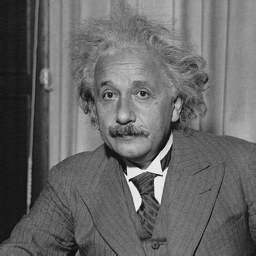
\includegraphics[width=\mywidth]{metrics/reference}};
		\draw (ref) to [out=-10, in=30] ++(2.5, -1) node [below] {\( x \)};
		\draw [ultra thick] (0, 0) circle (\myrad);
		\draw (2, -5.8) to [out=-80, in=140] ++(.5, -1.5) node [right] {\( \Set{y \in \R^{\numproduct{256x256}} \given \norm{x - y}_{\num{2}}^{\num{2}} = r^\prime} \)};
		\foreach [count=\iname] \nname in {mean, contrast, impulse, blur, jpeg}{%
			% + 36 just to offset it
			\pgfmathsetlengthmacro{\xx}{cos(\iname * 360 / 5 + 36) * \myrad}
			\pgfmathsetlengthmacro{\yy}{sin(\iname * 360 / 5 + 26) * \myrad}
			\node at (\xx, \yy) {\includegraphics[width=\mywidth]{metrics/\nname}};
			\pgfmathsetlengthmacro{\yyanno}{\yy + \mywidth/2+.3cm}
			\node at (\xx, \yyanno) {\( \hat{x}_{\iname} \)};
			\pgfmathsetlengthmacro{\xxssim}{\xx - 1.9cm}
			\pgfmathsetlengthmacro{\yyssim}{\yy + 1.6cm}
			\pgfmathsetmacro{\ssim}{\ssims[\iname-1]}
			\node [right, rounded corners, fill=white] at (\xxssim, \yyssim) {\ifthenelse{\iname=1}{SSIM=}{}\num{\ssim}};
		}
	\end{tikzpicture}
	\caption[Images on the MSE hypersphere appear vastly different to the human]{%
		The corrupted images \( \hat{x}_{\num{1}},\dotsc,\hat{x}_{\num{5}} \) all have the same \gls{mse} with respect to the reference image \( x \).
		However, to a human they appear vastly different.
		The image \( x_{\num{1}} \), where the same constant offset is added to each pixel, is \enquote{the same} as the original image \( x \) to the human observer.
		On the other hand, the image \( x_{\num{5}} \), which has undergone severe JPEG compression, has lost many details and looks much worse to the human.
		The inlays show the \glsxtrshort{ssim} value (the images are ordered in decreasing \glsxtrshort{ssim} counterclockwise from twelve o'clock), which align much closer with human assessment.
	}%
	\label{fig:mse doesnt correspond to human visual assessment}
\end{figure*}
This discrepancy poses a problem if the output of an algorithm is presented to a human, for instance, for diagnosis or entertainment.

Numerous quality metrics have been proposed to address this issue and we refer to~\cite{mason_imagequality_2020} for a small overview and a study of how well quality metrics predict radiologists' performance.
In this thesis, we use the popular \gls{ssim}.
The definition of the \gls{ssim} is understood locally on small patches; the image-level metric is the mean over all overlapping patches, with a filter to avoid blocking artifacts.
\begin{definition}[Structural similarity]%
	\label{def:ssim}
	Let \( x, \hat{x} \in \R^{d \times d} \) be two image patches and let \( \mu_{x}, \mu_{\hat{x}} \in \R \) and \( \sigma_x, \sigma_{\hat{x}} > \num{0} \) be their mean and standard deviation respectively, e.g.\ \( \mu_{x} = \tfrac{1}{d^{\num{2}}} \sum_{i,j=\num{1}}^{d,d} x_{i,j} \) and \( \sigma_x^{\num{2}} = \frac{1}{d^{\num{2}}-\num{1}} \sum_{i,j=\num{1}}^{d,d} (x_{i,j} - \mu_x)^{\num{2}} \).
	In addition, let \( \operatorname{cov}_{x\hat{x}} = \frac{1}{d^{\num{2}}-1} \sum_{i,j=\num{1}}^{d,d} (x_{i,j}- \mu_x)(\hat{x}_{i,j} - \mu_{\hat{x}}) \) and let \( K_{\num{1}} > \num{0} \) and \( K_{\num{2}} > \num{0} \).
	The \emph{\glsxtrlong{ssim}} between \( x \) and \( \hat{x} \) is
	\begin{equation}
		\frac{(\num{2}\mu_x\mu_{\hat{x}} + C_{\num{1}})(\num{2}\operatorname{cov}_{x\hat{x}} + C_{\num{2}})}{(\mu_x^{\num{2}}+\mu_{\hat{x}}^{\num{2}} + C_{\num{1}})(\sigma_x^{\num{2}} + \sigma_{\hat{x}}^{\num{2}} + C_{\num{2}})}
	\end{equation}
	where \( C_{\num{1}} = (K_{\num{1}}m)^{\num{2}} \) and \( C_{\num{2}} = (K_{\num{2}}m)^{\num{2}} \) with \( \MaxIntensity \in \R \) defined as in~\cref{def:psnr}.
\end{definition}

\Gls{ssim} can be decomposed into components comparing \enquote{luminance}, \enquote{contrast}, and \enquote{structure}, for details see the original publication~\cite{wang_ssim_2004}.
In this thesis, we use a \numproduct{7x7} uniform filter\footnote{%
	This means that, in the above definition, \( d = \num{7} \) and the image patches are essentially taken directly (without filtering).%
} and standard choices \( K_{\num{1}} = \num{0.01} \) and \( K_{\num{2}} = \num{0.03} \).
As for the \gls{psnr}, when the highest pixel intensity is not well defined, we take the highest pixel intensity in the reference image.
\Cref{fig:mse doesnt correspond to human visual assessment} shows \gls{ssim} as inlays; with images ordered in decreasing \gls{ssim} (counterclockwise from twelve o'clock), demonstrating that \gls{ssim} provides a better alignment with human assessment.

\chapter{Machine learning}%
\label{chap:machine-learning}%
\graphicspath{{./chapters/machine-learning/scripts}}%
In \marginnote{\footnotesize \textbf{Contents:}\\\localtableofcontents}this chapter we define \glspl{nn} and their building blocks, including convolutional layers and popular nonlinearities, and discuss the implications of their nonsmoothness.
We then outline our notions of supervised and unsupervised learning as well as generative versus discriminative learning.
This chapter is intended to set the stage for the subsequent chapters and is not a comprehensive introduction to these concepts.
For a broader overview, refer to~\cite{bishop_pattern_2006}.
\section{Neural networks}%
\label{sec:neural networks}
In this thesis, we adopt a broad interpretation of the term \enquote{\gls{nn}}.
We consider all functions with the following characteristics as \glspl{nn}:
First, a neural network is a \emph{parametric} function, with parameters that we \emph{learn} from data.
Second, these functions follow a particular structure.
The term neural network implies that the architecture of these functions is (loosely) inspired by the structure of the brain, where electrical signals from spikes of neighboring neurons are weighted and summed.
When the electric potential in the neuron exceeds a threshold, it releases a spike.\footnote{%
	We are not considering spiking neural networks in this thesis.
	This interpretation is just to motivate the following discussion.
}
Thus, the inputs to the neuron are combined \emph{linearly}, and the output of the neuron is a \emph{nonlinear activation function}.\footnote{%
	In this chapter, we borrow the terminology from the neural network community.
	In~\cref{chap:pogmdm}, we borrow the terminology from the \glsxtrlong{mrf} community.
	There, these activation functions are called \emph{potentials}, whose derivatives are the \emph{activations}.
}
Then, the next layer of neurons downstream of the output proceeds similarly, creating a \emph{layered} structure of linear weightings and a non-linear functions acting on individual neurons.

In this analogy, the learnable parameters are the weights of the inputs, and possible parameters of the activation function.
In most contemporary neural network literature, the activation functions are chosen a-priori and seen as fixed.\footnote{%
	Arguably, this changes with the recent introduction of Kolmogorov-Arnold networks~\cite{liu2024kan}.
}
However, the models in~\cref{chap:pogmdm} have \emph{learnable} activation functions when viewed in this framework.
Specifically, these models can be regarded as one-layer neural networks with trainable activation functions that are the negative logarithm of a one-dimensional \gls{gmm}.

We formalize the layered structure of \glspl{nn} as follows:
Let \( \mathcal{X} \) be the input space and \( \Theta \) the set of admissible parameters.
In this thesis, the input space is always (at least isomorphic to) \( \R^n \).
For example, grayscale images of size \( \Height \times \Width \) make \( \mathcal{X} = \R^{\Height\times\Width} \).
The set of admissible parameters \( \Theta \) encodes the space of all learnable parameters, with possible constraints.
For example, learning \( \NumExperts \in \mathbb{N} \) convolution filters of size \( b \times b \) gives \( \Theta = \R^{b \times b \times \NumExperts} \).
In imaging applications, invariance with respect to radiometric shift is often desired and translates to a zero-mean constraint on the filters, then \( \Theta = \Set{x \in \R^{b \times b \times \NumExperts} \given \sum_{i, j=1}^{b,b} x_{i, j, k} = \num{0}\ \text{for all}\ k = \num{1}, \dotsc, \NumExperts} \).

Irrespective of input and parameter spaces, a \gls{nn} is a map \( f \)  from \( \mathcal{X} \times \Theta \) to the output space \( \mathcal{Y} \):
\begin{equation}
	\map{f}{\mathcal{X} \times \Theta}{\mathcal{Y}}.
\end{equation}
The output space depends on the task:
It could be the \( k \)-dimensional unit simplex \( \Simplex^k \) (\cref{def:unit simplex}) for \( k \)-class classification~\cite{OU20074}, or the input space \( \mathcal{X} \) when the \gls{nn} models the gradient of an unknown real-valued function of the input~\cite{chung_scoremri_2022,song2021scorebased}.\footnote{%
	This real-valued function could be related to the density of some reference distribution, as is the case in \cref{chap:deep neural regularizers} and \cref{chap:pogmdm} in this thesis.
}
In the applications we focus on, the output space is \( \mathbb{R} \), meaning the \gls{nn} maps its input to a scalar.
This scalar indicates whether the input to the \gls{nn} is \enquote{likely} under some reference distribution learned by \gls{nn}.
\Cref{fig:neural network examples} shows examples of how neural networks are used for different tasks.
\begin{figure*}
	\begin{tikzpicture}
		\begin{scope}[xshift=0cm]
			\node at (0.5, 2.4) {\( f_{c}(\,\cdot\,,\Theta_{c}) : \)};
			\node at (-1.3, 1.7) {\( \mathbb{R}^{28 \times 28} \)};
			\node at (1.8, 1.7) {\( \Simplex^5 : \)};
			\draw [->] (0, 1.7) -- ++(1., 0);
			\node at (-1.3, 0) {
\includegraphics[width=2cm]{mnist/00}};
			\draw [|->] (0, 0) -- (1.0, 0);
			\node at (1.7, 0) {\( \begin{pmatrix}.1\\.1\\.1\\.1\\.6\end{pmatrix} \)};
			\begin{scope}[yshift=-2.5cm]
				\node at (-1.3, 0) {
\includegraphics[width=2cm]{mnist/noisy}};
				\draw [|->] (0, 0) -- (1.0, 0);
				\node at (1.7, 0) {\( \begin{pmatrix}.2\\.1\\.2\\.2\\.3\end{pmatrix} \)};
			\end{scope}
			\node at (.0, -4) {Classification};
		\end{scope}
		\begin{scope}[xshift=5.3cm]
			\node at (0.5, 2.4) {\( f_{n}(\,\cdot\,,\Theta_{n}) : \)};
			\node at (-1.4, 1.7) {\( \mathbb{R}^{28 \times 28} \)};
			\node at (2.4, 1.7) {\(  \mathbb{R}^{28 \times 28} : \)};
			\draw [->] (0, 1.7) -- ++(1., 0);
			\draw [|->] (0, 0) -- ++(1., 0);
			\node at (-1.3, 0) {
\includegraphics[width=2cm]{mnist/00}};
			\node at (2.4, 0) {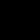
\includegraphics[width=2cm]{mnist/nonoise}};
			\begin{scope}[yshift=-2.5cm]
				\node at (-1.3, 0) {
\includegraphics[width=2cm]{mnist/noisy}};
				\node at (2.4, 0) {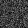
\includegraphics[width=2cm]{mnist/noise}};
				\draw [|->] (0, 0) -- ++(1., 0);
			\end{scope}
			\fill [gray] (-2.95, -4.3) rectangle ++(.1, 6.8);
			\node at (.5, -4) {Noise estimation};
		\end{scope}
		\begin{scope}[xshift=11.8cm]
			\node at (0.5, 2.4) {\( f_{l}(\,\cdot\,,\Theta_{l}) : \)};
			\node at (-1.3, 1.7) {\( \mathbb{R}^{28 \times 28} \)};
			\node at (1.7, 1.7) {\(  \mathbb{R} : \)};
			\draw [->] (0, 1.7) -- ++(1., 0);
			\draw [|->] (0, 0) -- ++(1., 0);
			\node at (-1.3, 0) {
\includegraphics[width=2cm]{mnist/00}};
			\node at (1.7, 0) {4.5};
			\begin{scope}[yshift=-2.5cm]
				\node at (1.7, 0) {1.3};
				\node at (-1.3, 0) {
\includegraphics[width=2cm]{mnist/noisy}};
				\draw [|->] (0, 0) -- ++(1., 0);
			\end{scope}
			\fill [gray] (-2.85, -4.3) rectangle ++(.1, 6.8);
			\node at (.0, -4) {Likelihood estimation};
		\end{scope}
	\end{tikzpicture}
	\caption[Example applications of neural networks]{%
		Examples of neural networks:
		In the five-class classification problem on the left, the neural network \( f_c(\argm, \Theta_c) \) maps from the input space, images of size \numproduct{28x28} with real pixels, to the five-dimensional unit simplex.
		The entries of a vector which is an element of the five-dimensional unit simplex can be interpreted as probabilities.
		The goal here is (loosely speaking) that the correct class (here class \enquote{5}) has the highest probability.
		In the noise estimation problem in the middle, the neural network \( f_n(\argm, \Theta_n) \) maps from the input space to itself;
		An estimate of a noise-free image could be given by subtracting the output of the neural network from the input.
		In the likelihood estimation problem on the right, the neural network \( f_l(\argm, \Theta_l) \) maps from the input space to the real line.
		Here, the real number that is assigned to an input reflects its likelihood under the learned model.
		Although the noise- and likelihood estimation problem seem unrelated, there is an extremely close connection via Tweedie's identity.
		We discuss this in more detail in~\cref{chap:pogmdm}.
	}%
	\label{fig:neural network examples}
\end{figure*}

We now explore the \emph{architecture} of \glspl{nn}, recalling some concepts needed later.
A \gls{nn} \( f \) typically consists of a cascade of composed functions.
Specifically, an \emph{\( L \)-layer network} is structured as
\begin{equation}
	f = f_L \composed f_{L-\num{1}} \composed \cdots \composed f_{\num{2}} \composed f_{\num{1}}.
	\label{eq:neural network composition}
\end{equation}
Each layer \( \map{f_i}{\mathcal{X}_{i-\num{1}} \times \Theta_i}{\mathcal{X}_{i}} \) for \( i = \num{1}, \dotsc, L \) can be decomposed into a linear map followed by a point-wise non-linearity, and typically has its own parameters in the parameter space \( \Theta_i \subseteq \Theta \).\footnote{%
	We say subset of or equal to because the \gls{nn} may only have one parametrized layer.
}
An \( L \)-layer network is often referred to as having a \emph{depth} of \( L \), with all layers between the input and the output considered \emph{hidden}.

In the next section, we provide more detail on the linear and non-linear elements that constitute a layer.
Specifically, within the context of image processing, we explore \emph{convolutional layers} and some of the most popular nonlinearities.
The architectures and building blocks we use in this thesis are relatively straightforward.
For a more comprehensive review, see Cong and Zhou's survey~\cite{Cong2022}.
\subsection{Linear layers}
The linear sub-layers in \glspl{nn} are general affine maps.
Formally, let \( \mathcal{X}_l \) and \( \mathcal{X}_{l+1} \) represent the input and output spaces of layer \( f_l \).
The linear sub-layer within \( f_l \) is the affine map
\begin{equation}
	\mathcal{X}_l \times \Theta_l \ni (x, \theta) \mapsto K_lx + b_l
\end{equation}
where \( \map{K_l}{\mathcal{X}_l}{\mathcal{X}_{l + \num{1}}} \) is an arbitrary linear operator, and \( b_l \in \mathcal{X}_{l + \num{1}} \) is the affine offset, commonly referred to as \emph{bias} in the \gls{nn} literature.
The parameters \( \theta_l \) could be all weights in \( K_l \) and entries in \( b_l \).
However, often \( K_l \) and \( b_l \) are derived from a much lower dimensional object.
For example, the operator \( K_l \) can model the convolution of the input with the convolution kernels encoded in the entries of \( \theta \).

This thesis considers two primary types of linear sub-layers:
dense and fully-learned operators, and convolution operators.
These are particularly relevant in imaging applications.
Dense linear operators are useful for \enquote{inverting} imaging transforms such as the Fourier or the Radon transform.
Conversely, convolutions are crucial due to their inherent translation equivariance which is often desired in imaging tasks.

Sub-layers employing dense, fully-learnable operators are typically called \emph{fully connected}.
Here, the learnable parameters are \emph{all} weights in \( K_l \) and entries in \( b \).
In imaging applications, this can be extremely memory intensive:
Consider an image \( x \) of size \( \Height \times \Width \) with three color channels, i.e., \( x \in \R^{\Height \times \Width \times \num{3}} \) and assume we want to learn a linear operator that maps from this space to itself.
This linear operator has \( (\Height \times \Width \times \num{3}) \times (\Height \times \Width \times \num{3}) \) weights.
For a \( \Height = \Width = \num{256} \) square image, this amounts to \num{38654705664} weights, requiring more than \qty{154}{\giga\byte} of storage as \num{32}-bit floating-point numbers.
We use a fully connected layer as the last layer in our deep neural regularizer discussed in~\cref{chap:deep neural regularizers}.
There, the output space is a scalar and consequently the number of learnable parameters in the fully connected layer is equal to the dimensionality of its input space.

In imaging applications, \emph{convolution layers} are especially important.
Unlike fully connected layers, not all weights in the linear operator are learnable.
Instead, the operator's weights are derived from a learnable \emph{kernel} and the operator is constructed to encode a convolution.
Let \( x \in \mathcal{X}_{l-\num{1}} = \R^{c_{l-\num{1}} \times \Height_{l-\num{1}} \times \Width_{l-\num{1}}} \) be the input the \( l \)-th layer of the \gls{nn}.
In image processing, \( c_{l-\num{1}} \in \mathbb{N} \) are \emph{features} or \emph{channels} of the (\( l - \num{1} \))-th layer.
If the \( l \)-th layer has \( c_l \) features, the linear operator is a map \( \map{K_l}{\R^{c_{l-\num{1}} \times \Height_{l-\num{1}} \times \Width_{l-\num{1}}}}{\R^{c_{l} \times \Height_{l-\num{1}} \times \Width_{l-\num{1}}}} \), i.e.\ the size of the features remains unchanged.
The application of the linear operator is described by a total of \( c_{l-\num{1}} c_l\) convolutions.
Formally, let \( k^l_{c, d} \in \R^{s \times s} \) be a kernel of size \( s \times s \) where \( \num{1} \leq c \leq c_{l-\num{1}} \) and \( \num{1} \leq d \leq c_{\num{1}} \).
Then, the application of the linear operator \( K_l \) is described by
\begin{equation}
	(K_l x)_{c, i, j} = \sum_{d=\num{1}}^{c_{l-\num{1}}} \sum_{a,b=\num{1}}^{s,s} (k^l_{c, d})_{a, b} \cdot x_{d, \operatorname{bdy}(i - a + \lfloor s / \num{2} \rfloor, \Height_{l-1}), \operatorname{bdy}(j - b + \lfloor s / \num{2} \rfloor, \Width_{l-\num{1}})}.
\end{equation}
Here, the map \( \map{\operatorname{bdy}}{\mathbb{N} \times \mathbb{N}}{\mathbb{N}} \) can be used to realize different boundary conditions when \( \num{0} < i - a + \lfloor s / \num{2} \rfloor \leq \Height_{l-\num{1}} \) or \( \num{0} < j - b + \lfloor s / \num{2} \rfloor \leq \Width_{l-\num{1}} \) do not hold, see~\cref{ssec:convolutions}.
In the context of this thesis, the most important technique is \emph{periodic} or \emph{circular} boundary handling due to its relations with the Fourier transform.
There, the signals are assumed to be \( (\Height_{l-\num{1}}, \Width_{l-\num{1}}) \)-periodic, i.e.\ \( \operatorname{bdy} \) is given by\footnote{%
	This is written in array-notation with one-based indexing.
	A more familiar form is simply \( a \mod b \) for sequence-notation with zero-based indexing.
}
\begin{equation}
	(a, b) \mapsto (a + (b - \num{1}) \mod b) + \num{1}.
\end{equation}
In this case, we can make use of the \emph{convolution theorem} to diagonalize the linear operator \( K_l \) using the Fourier transform, see~\cref{chap:pogmdm}.

To expand the receptive field of subsequent layers, neural networks often integrate \emph{downsampling} layers.
It suffices to describe the action of downsampling layers on one channel; the application to multiple channels is channel-wise.
Applying a \( d \)-fold downsampling layer to an image of size \( \Height \times \Width \) results in an output image of size \( \frac{\Height}{d} \times \frac{\Width}{d} \) as illustrated in~\cref{fig:downsampling}.
There, every \( d \)-th pixel is copied into the output and consequently downsampling layers have no learnable parameters.
\begin{sidefigure}
	\centering
	\begin{tikzpicture}[every node/.style={anchor=center,inner sep=0, thick, draw, minimum size=5mm},]
		\matrix [matrix of nodes,column sep=0mm,row sep=0mm] (input)
		{
			\textcolor{maincolor}{8} & 1 & \textcolor{maincolor}{6} & 8 \\
			3 & 5 & 7 & 9 \\
			\textcolor{maincolor}{4} & 9 & \textcolor{maincolor}{2} & 5 \\
			9 & 4 & 5 & 6 \\ 
		};
		\matrix [below=of input, matrix of nodes,column sep=0mm,row sep=0mm]
		{
			\textcolor{maincolor}{8} & \textcolor{maincolor}{6} \\
			\textcolor{maincolor}{4} & \textcolor{maincolor}{2} \\
		};
	\end{tikzpicture}
	\caption[Action of a downsampling layer]{Visualization of a \num{2}-fold downsampling operation.}
	\label{fig:downsampling}
\end{sidefigure}
A practical implementation of downsampling involves merging convolution and downsampling operations into \emph{strided convolutions}, minimizing unnecessary computations.
\subsection{Nonlinearities}
\label{ssec:nonlinearities}
Composing only linear layers would result in an overall linear function, which is insufficient for many tasks and famously fails to solve the \enquote{XOR} problem.
Thus, in order for the composition~\cref{eq:neural network composition} to become any stronger than linear, the layers must incorporate nonlinearities.

Nonlinearities in \glspl{nn} typically act point-wise.
Formally, assume that the linear sub-layer in the \( l \)-th layer (which is not the output layer) maps to \( \tilde{\mathcal{X}}_l = \R^{f_l \times \Height_l \times \Width_l} \).
The nonlinear sub-layer is a function \( \map{\Phi_l}{\tilde{\mathcal{X}}_l}{\tilde{\mathcal{X}}_l} \) often structured such that it applies the same function \( \map{\phi_l}{\R}{\R} \) point-wise:
\begin{equation}
	\bigl(\Phi_l(x)\bigr)_{i, j, k} = \phi_l(x_{i, j, k})
	\label{eq:shared pointwise nonlinearity}
\end{equation}
and often the scalar function \( \phi_l \) is also shared between all layers.
The output space of the \( i \)-th nonlinear sub-layer is the input space of the (\( i + \num{1} \))-th layer, i.e., \( \mathcal{X}_{i + \num{1}} = \tilde{\mathcal{X}}_l \).

Numerous activation functions have been proposed in the literature;
for a relatively recent and comprehensive overview see~\cite{dubey_activation_2022}.
Popular examples include the logistic sigmoid \( x \mapsto (\num{1} + \exp(-x))^{\num{-1}} \) and the hyperbolic tangent \( x \mapsto \frac{\exp(x) - \exp(-x)}{\exp(x) - \exp(-x)} \).
However, these suffer from vanishing or exploding gradients.
The rectified linear unit \( \relu = (x \mapsto \max(\num{0}, x)) \) has become a favored choice to mitigate this.
While \( \relu \) is not differentiable at \( \num{0} \), automatic differentiation frameworks such as PyTorch~\cite{paszke_pytorch_2019}, handle this by choosing an element of the subdifferential at \( \num{0} \), usually \( \num{0} \).
However, an implicit differentiation framework that encompasses nonsmooth functions has been missing until relatively recently.
In 2021, Bolte et al. introduced the notion of \emph{path differentiability} in~\cite{bolte_nonsmooth_implicit_2021} which aims to resolve this problem.

The nondifferentiability of \( \relu \) poses a challenge for classical optimization algorithms.
We optimize our learned networks (w.r.t.\ their input) in~\cref{chap:deep neural regularizers} with standard first-order optimization methods discussed in~\cref{ssec:nonconvex optimization}.
While optimization works well empirically, we can not guarantee convergence.
Surrogates for \( \relu \) such as the swish \( x \mapsto \frac{x}{\num{1} + \exp(-x)} \) or the exponential linear unit
\[
	x \mapsto \begin{cases}
		x &\ \text{if}\ x > \num{0}, \\
		\exp(x) - \num{1} &\ \text{else},
	\end{cases}
\]
offer differentiable alternatives.
If one wants to avoid the computational complexity of these functions during training but ensure convergence of optimization algorithms, it is possible to replace the rectified linear activation functions with a differentiable counterpart after training.
However, in order for the learned parameters to be meaningful, the surrogate must approximate \( \relu \) well, and the gradient of any reasonable approximation will necessarily have an exploding Lipschitz constant, effecting optimization speed.

In~\cref{chap:regularizers} we use a \emph{leaky} rectified linear activation given by
\begin{equation}
	\relu = x \mapsto \max(\gamma x, x)
\end{equation}
with the small leakage coefficient \( \gamma > \num{0} \).
The discussion about nondifferentiability, its implications, and possible remedies carries over to this version.
\Cref{fig:nonlinearities} showcases a selection of popular nonlinearities.
\begin{sidefigure}
	\begin{tikzpicture}[declare function={
		lrelu(\x,\g)=max(\g*\x, \x);
		elu(\x)=(x > 0) * x + (x < 0) * (exp(x) - 1);
		swish(\x)=\x/(1 + exp(-\x));
		sigmoid(\x)=1/(1 + exp(-\x));
	}]
		\begin{axis}[domain=-2:2, marginplot, xmin=-2, xmax=2, no markers]
			\addplot+ [thick] {elu(x)};
			\addplot+ [thick] {lrelu(x, 0)};
			\addplot+ [thick] {lrelu(x, 0.1)};
			\addplot+ [thick] {swish(x)};
			\addplot+ [thick] {sigmoid(x)};
		\end{axis}
	\end{tikzpicture}
	\caption[Common nonlinearities in neural networks]{%
		\tikzexternaldisable
		Common nonlinearities in neural networks:
		The exponential linear unit %
		\protect\tikz[baseline=-\the\dimexpr\fontdimen22\textfont2\relax]\protect\draw [index of colormap={0} of flare, thick] (0,0) -- (.5, 0);,
		the rectified linear unit %
		\protect\tikz[baseline=-\the\dimexpr\fontdimen22\textfont2\relax]\protect\draw [index of colormap={4} of flare, thick] (0,0) -- (.5, 0); %
		and its leaky variant %
		\protect\tikz[baseline=-\the\dimexpr\fontdimen22\textfont2\relax]\protect\draw [index of colormap={8} of flare, thick] (0,0) -- (.5, 0);, %
		the swish %
		\protect\tikz[baseline=-\the\dimexpr\fontdimen22\textfont2\relax]\protect\draw [index of colormap={12} of flare, thick] (0,0) -- (.5, 0);, %
		and the sigmoid %
		\protect\tikz[baseline=-\the\dimexpr\fontdimen22\textfont2\relax]\protect\draw [index of colormap={17} of flare, thick] (0,0) -- (.5, 0);.
		\tikzexternalenable
	}%
	\label{fig:nonlinearities}
\end{sidefigure}

The choice of nonlinearity in the output layer depends on the task and is not necessarily point-wise.
For instance, in \( K \)-class classification problems, the soft-argmax\footnote{%
	This is sometimes given the misleading name \enquote{softmax}.
	However, it smoothly approximates the argmax function, not the maximum.
}
\begin{equation}
	\R^K \ni (x_{\num{1}}, \dotsc, x_K) \mapsto \begin{pmatrix}
		\frac{\exp(x_i)}{\sum_{i=\num{1}}^K\exp(x_i)}\\
		\vdots\\
		\frac{\exp(x_i)}{\sum_{i=\num{1}}^K\exp(x_i)}
	\end{pmatrix}.
\end{equation}
is a popular choice.
It maps any point onto the \( K \)-dimensional unit simplex \( \Simplex^K \) and hence its output values can be interpreted as probabilities.
Depending on the application, the identity map \( x \mapsto x \) may be suitable, making the output of the network the output of the last linear sub-layer.

The models we discuss in~\cref{chap:pogmdm} can be viewed as one-layer networks, with each of the \( \NumExperts \in \mathbb{N} \) convolution operators equipped with their own scalar-valued activation function.
Thus, \( \Phi \) has the block structure
\begin{equation}
	\R^{\Height \times \Width \times \NumExperts} \ni (x_{\num{1}}, \dotsc, x_{\NumExperts}) \mapsto (\Phi_{\num{1}}(x_{\num{1}}), \dotsc, \Phi_\NumExperts(x_\NumExperts))
\end{equation}
where each \( \map{\Phi_i}{\R^{m \times n}}{{\R^{m\times n}}} \) shares the same \( \map{\phi_i}{\R}{\R} \) across all \( i = \num{1}, \dotsc, \NumExperts \).
The nonlinearities are log-sum-exp functions, interpreted as the negative logarithm of a probability density function parametrized through a \gls{gmm}.
Thus, the nonlinearities are endowed with parameters that we \emph{learn} from data.
\section{Supervised and unsupervised learning}
Machine learning approaches are classically divided into \emph{supervised learning} and \emph{unsupervised learning}~\cite{bishop_pattern_2006}.
In this section, we elaborate on the differences between these two approaches.

In \emph{supervised learning}, we are given a reference dataset of (input, output) pairs, and the goal is to learn a parametric map that accurately reproduces the reference output for a given input.
Formally, consider a pair \( (X, Y) \) of random variables, where \( Y \) is the input random variable with values in \( \mathcal{Y} \), and \( X \) is the output random variable with values in \( \mathcal{X} \).
Here, we adopt the notation from the introduction and the rest of the thesis which is in contrast to the previous section; there the input and output spaces are flipped.
We assume that the pair \( (X, Y) \) is distributed as \( p_{X, Y} \).

The objective is to learn a parametric map
\begin{equation}
	\map{f}{\mathcal{Y} \times \Theta}{\mathcal{X}}
\end{equation}
that maps an input \( y \in \mathcal{Y} \) to \( f(y, \theta) \in \mathcal{X} \) given parameters \( \theta \in \Theta \).
The set of admissible parameters \( \Theta \) can encode constraints on the parameter vector \( \theta \), e.g.\ to enforce invariances.
To find optimal parameters, we minimize a loss function \( \map{l}{\mathcal{X} \times \mathcal{X}} \) that compares two points in the output space \( \mathcal{X} \):
\begin{equation}
	\min_{\theta \in \Theta}\Expectation_{(X, Y)\sim p_{X,Y}}\bigl[ l(f(Y, \theta), X) \bigr].
\end{equation}

Supervised learning encompasses classification, where the output space is discrete, and regression, where the output space is continuous.
Examples of the former include classification problems in computer vision, such as semantic segmentation or object detection, but also problems like spam detection or bot detection.
Examples of the latter include polynomial regression, stock price prediction, and image reconstruction.

In \emph{unsupervised learning}, we aim to find structure in the distribution of the \emph{input} random variable \( Y \).
A prototypical example is \emph{density estimation}, which aims to fit a parametric model to the density of the random variable.
This is often formalized as maximum likelihood learning, which amounts to finding parameters \( \theta \) of a parametric density \( \map{p}{\mathcal{Y} \times \theta}{\interval{\num{0}}{\infty}} \) via
\begin{equation}
	\min_{\theta \in \Theta} \Expectation_{Y \sim \DensityFunction_Y}\bigl[ -\log p(Y, \theta) \bigr].
\end{equation}
\begin{sidefigure}
	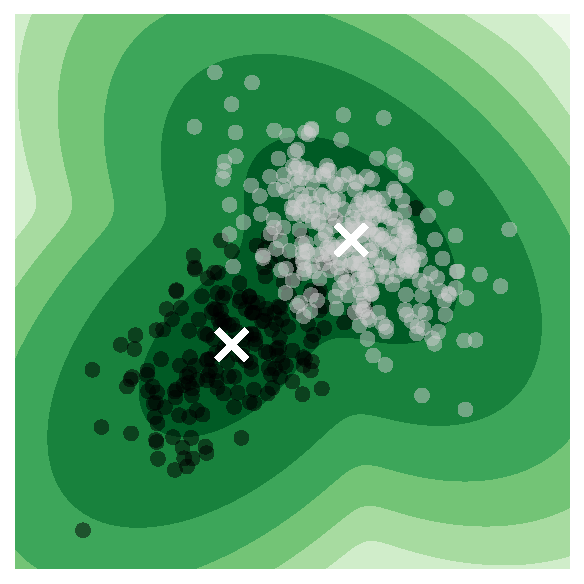
\includegraphics[width=\marginparwidth]{learning-types/gmm}
	\caption[Unsupervised learning: Density estimation]{
		Density estimation of a point cloud with a Gaussian mixture model.
		The white crosses indicate the means of the two components and the shades of green indicate the density.
	}%
	\label{fig:unsupervised gmm}
\end{sidefigure}

Another classic unsupervised task is \emph{clustering}, where the aim is to partition the input space into disjoint regions based on an unlabeled dataset.
A query point can then be assigned to one of the clusters based on its region.
Fixing the number of clusters to \( K \) and constructing the disjoint regions such that the Euclidean distance between points in the regions is minimized leads to the famous \( K \)-means algorithm~\cite{lloyd_least_1982}.
\begin{sidefigure}
	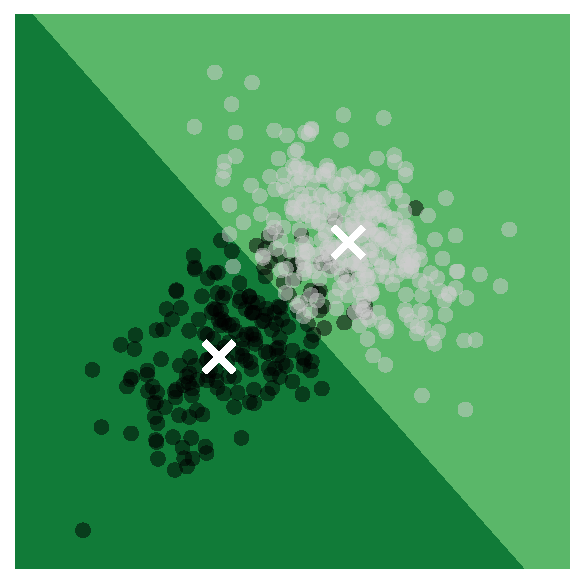
\includegraphics[width=\marginparwidth]{learning-types/km}
	\caption[Unsupervised learning: Clustering]{
		Clustering of a point cloud with K-means.
		The white crosses indicate the centroids of the two clusters and the shades of green indicate the cluster a point is assigned to.
	}%
	\label{fig:unsupervised km}
\end{sidefigure}
\Cref{fig:unsupervised gmm} and \cref{fig:unsupervised km} show examples of density estimation with a Gaussian mixture model and clustering with the K-means algorithm on a point cloud drawn from two Gaussians in two dimensions.
\section{Generative and discriminative learning}
This thesis focuses on using \emph{generative learning} for inverse problems in imaging.
Here, we distinguish between generative and discriminative learning by considering a supervised estimation problem.
Consider a pair of random variables \( (X, Y) \) with joint distribution \( p_{X, Y } \) and marginal distributions \( p_X \) and \( p_Y \).
As in the previous section, \( Y \) is the \emph{input} random variable and \( X \) is the output random variable.

In the \emph{discriminative approach}, the joint distribution is factorized as
\begin{equation}
	p_{X, Y} = p_{X\mid Y} p_Y,
\end{equation}
where \( p_{X\mid Y} \) is the \emph{posterior} of the output given the input and \( p_Y \) is the density of the input.
Training parametric estimators of this type\footnote{%
	in the standard maximum-likelihood framework; the conclusions also hold for more general formulations.
} amounts to finding
\begin{equation}
	\min_{\theta_{X \mid Y}, \theta_Y} \Expectation_{(X, Y) \sim p_{X, Y}}\bigl[ -\log \hat{p}_{X\mid Y}(X, Y, \theta_{X\mid Y}) \bigr] + \Expectation_{Y \sim p_Y} \bigl[ -\log \hat{p}_Y(Y, \theta_Y) \bigr],
\end{equation}
where  \( \hat{p}_{X\mid Y}(\argm,\argm,\theta_{X\mid Y}) \) and \( \hat{p}_Y(\argm, \theta_Y) \) are parametric estimators.
Thus, the discriminative approach decouples into the posterior and the input density.

For practical inference problems, the parametric posterior suffices:
Given an input \( y \in \mathcal{Y} \), the associated estimation of the output can be found via\footnote{For the sake of simplicity, we only discuss \gls{map} estimation}
\begin{equation}
	\argmax_{x \in \mathcal{X}} \hat{p}_{X \mid Y} (x, y, \theta_{X \mid Y}).
\end{equation}
The discriminative approach has the advantage that the parametric posterior is typically simpler than the density of the output; see the example below.
However, it is challenging to encode domain knowledge and it is typically impossible to adapt to changes in the relationship between the input and output random variables;
we demonstrate this with an example in \gls{mri} in~\cref{sec:discriminative pitfalls}.

In the \emph{generative approach}, the joint distribution is factorized as
\begin{equation}
	p_{X, Y} = p_{Y \mid X} p_X,
\end{equation}
where \( p_{Y \mid X} \) is the \emph{likelihood} of an input given an output, and \( p_X \) is the density of the output.
Training parametric estimators of this type amounts to finding
\begin{equation}
	\min_{\theta_{Y \mid X}, \theta_X} \Expectation_{(X, Y) \sim p_{X, Y}}\bigl[ -\log \hat{p}_{Y\mid X}(X, Y, \theta_{Y\mid X}) \bigr] + \Expectation_{X \sim p_X} \bigl[ -\log \hat{p}_X(X, \theta_X) \bigr],
\end{equation}
where \( \hat{p}_{Y \mid X}(\argm, \argm, \theta_{Y\mid X}) \) and \( \hat{p}_X(\argm, \theta_X) \) are parametric estimators.
When the parameters are learned, we can invoke Bayes theorem and write the posterior as
\begin{equation}
	\hat{p}_{X \mid Y} = \frac{\hat{p}_{Y \mid X}(\argm, \argm, \theta_{Y \mid X})\hat{p}_X(\argm, \theta_X)}{\hat{p}_Y}
\end{equation}
where the denominator is irrelevant with respect to the inference
\begin{equation}
	\argmax_{x \in \mathcal{X}} \hat{p}_{Y\mid X}(x, y, \theta_{Y \mid X}) \hat{p}_X(x, \theta_X).
\end{equation}
Thus, the generative approach separates the input likelihood from the output prior and invokes Bayes theorem for the posterior.

In this thesis, the likelihood is determined by the physical acquisition model and has extremely few parameters\footnote{usually one: the noise variance}, identified through grid search on a validation dataset.
Thus, the likelihood of \( Y \) given \( X \) is \emph{known, easy to model, and subject to change}.
Therefore, a generative learning approach is advantageous, as it allows for easy encoding of domain knowledge in the likelihood.
In addition, changes to the likelihood only require retraining of the parametric likelihood \( -\log \hat{p}_{Y \mid X}(\argm, \argm, \theta_{Y \mid X}) \).

In this taxonomy, \emph{supervised and unsupervised} as well as \emph{generative and discriminative} are understood with respect to the downstream task.
For example, in~\cref{chap:deep neural regularizers}, we learn a parametric form of the density of \gls{mri} images of the human knee.
For image reconstruction, this learned density represents the density of the \emph{output} random variable, making the approach \emph{generative} because it separates the input likelihood from the output prior.
However, it is \emph{supervised} because we train on the density of the output random variable.
For pathology detection\footnote{%
	With the learned density, pathology detection could for instance be implemented via simple likelihood evaluation.
}, this approach is \emph{unsupervised} (because there are no labels) but not generative:
Generative learning would amount to learning the density of the output random variable (essentially a scalar representing the pathologies prevalence), as well as the class conditional densities of images with and without pathologies.

We emphasize that discriminative learning is typically easier than generative learning through a two-class classification problem:
Assuming two normally distributed random variables with arbitrary mean and covariance, discriminative methods derive a parametric form of the posterior class density given a query point.
This object can famously be represented\footnote{%
	For either class; the posterior density for the other is just one minus the object.
} as (see, e.g.~\cite[section 4.2.1.]{bishop_pattern_2006})
\begin{equation}
	x \mapsto \bigl( \num{1} + \exp(\inprod{x}{Ax} + \inprod{b}{x} + c) \bigr)^{\num{-1}},
\end{equation}
where \( A \), \( b \), and \( c \) are a symmetric matrix, vector, and scalar, respectively.
For determining the most likely class, this simplifies further to identifying the parameters defining the hyperbolic decision boundary (depicted as a white line in~\cref{fig:discriminative}).
\begin{sidefigure}
	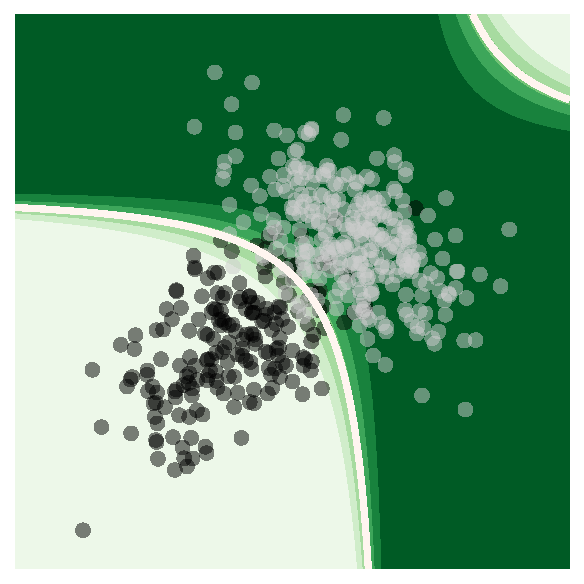
\includegraphics[width=\marginparwidth]{learning-types/discriminative}
	\caption[Discriminative two-class classification]{%
		Discriminative approach to the two-class classification problem:
		Darker green indicates higher posterior values of belonging to the \enquote{white} class.
		The white line is the hyperbolic decision boundary.
	}%
	\label{fig:discriminative}
\end{sidefigure}
In contrast, generative modeling finds the two class-conditional distributions, both general normal distributions, along with the class priors.
This requires estimating two symmetric positive definite matrices, two mean vectors and a scalar representing the class priors.
This is illustrated in~\cref{fig:generative}, where level lines are related to the covariance matrices and the size of the cross indicating the means is related to the class prior.
A new point is then classified according to its weighted likelihood.
\begin{sidefigure}
	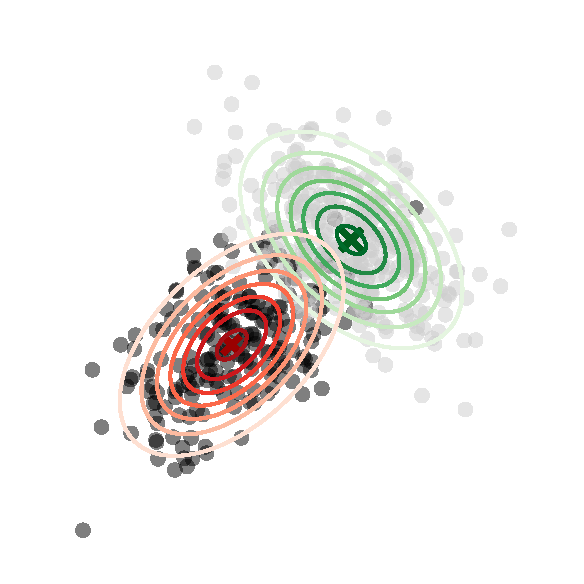
\includegraphics[width=\marginparwidth]{learning-types/generative}
	\caption[Generative two-class classification]{
		Generative approach to the two-class classification problem:
		The level lines are related to the covariance matrices, the size of the cross markers indicating the mean is related to the prior probability of a class.
		New points are classified according to the weighted likelihood; the decision boundary is shown in~\cref{fig:discriminative}.
	}%
	\label{fig:generative}
\end{sidefigure}

In the above example, the challenge lied mostly in finding the likelihood densities.
In this case, (for the purpose of pure classification) there is not merit to the generative approach.
However, in the inverse problems in imaging considered in this thesis, the likelihood of an input given an output is fixed by the physical acquisition model and is parameter-free up to scaling.
In addition, the physical acquisition model is subject to change:
As an example, in~\cref{chap:deep neural regularizers} we consider different frequency selections in a Fourier imaging setup.
On the other hand, the prior distribution of images is an extremely complicated object.
Thus, in this case the generative approach proves beneficial.
\Cref{chap:deep neural regularizers,chap:pogmdm} discuss two methods for learning a parametric density of image priors, highlighting the applicability of generative learning in such contexts.

\chapter{On the historical development of regularizers}%
\label{chap:regularizers}%
\graphicspath{{chapters/regularizers/scripts}}%
In \marginnote{\footnotesize \textbf{Contents:}\\\localtableofcontents}this chapter we outline the historical development of regularizers, starting with classical variational penalties such as magnitude or \gls{tv} penalties.
\gls{tv} regularization finds motivation in the histograms of natural images responses on finite difference filters, where the absolute value provides the best convex fit to the negative log-histograms.
This immediately suggests a generalization of this model:
a suitable set of filters, which can be readily computed from a set of reference images, is given by the principal directions of all image patches extracted from the reference images.
When sacrificing convexity, suitable potential functions are derived from the corresponding negative log-histograms.

However, despite their effectiveness in \gls{map} inference, these models do not account for the nontrivial correlation of overlapping patches, making them a bad model for the reference density.
In contrast, \gls{mrf} modeling accounts for this correlation.
By explicitly imposing translation invariance via convolutions, such models become very parameter efficient at the cost of a much more complex learning problem.
The \gls{pogmdm} discussed in~\cref{chap:pogmdm} exemplifies this approach.
Finally, the deep neural regularizer discussed in~\cref{chap:deep neural regularizers} models the reference density through a general map provided by a deep neural network.
Although sacrificing some interpretability and presenting an even more challenging learning problem, these models demonstrate excellent performance.

\section{A running example from MRI reconstruction}
To illustrate the historical development of regularizers, we employ a running example from \gls{mri} reconstruction.
However, the core focus of this chapter lies in examining \emph{the effect of the choice of the regularizer}.
For this purpose, we consider a simple reconstruction problem using synthetic data.
In contrast, much of \cref{chap:deep neural regularizers} is dedicated to developing clinically relevant reconstruction algorithms for real data.

We aim to reconstruct an image from Fourier data \( \Data \in \C^{f} \) constructed as
\begin{equation}
	\Data = \Mask \Fourier_{\R}\Signal + \Noise \coloneqq \Forward\Signal + \Noise,
\end{equation}
where \( x \in \R^{\Height \times \Width} \) represents the reference signal.
The two-dimensional \enquote{real} Fourier transform \( \map{\Fourier_{\R}}{\R^{\Height \times \Width}}{\C^{\Height \times (\lfloor \Width / \num{2} \rfloor + \num{1})}} \) exploits conjugate symmetry of the Fourier transform for real-valued signal by storing only half of the frequency plane.
Additionally, the Fourier transform is \emph{orthonormal}, i.e. that \( \Fourier_{\R}\Adjoint{\Fourier_{\R}} = \Adjoint{\Fourier_{\R}}\Fourier_{\R} = \Identity \).
The frequency selection operator\footnote{
	Other names for this object include \emph{undersampling mask} and \emph{subsampling-} or \emph{downsampling operator}.
} \( \map{\Mask}{\C^{\Height \times (\lfloor \Width / \num{2} \rfloor + \num{1})}}{\C^{f}} \) is a binary diagonal operator that selects \( f \in \mathbb{N} \) frequencies, simulating the \emph{acceleration} in clinical \gls{mri} systems (details in \cref{chap:deep neural regularizers}).
\( \Forward \) is a shorthand for \( \Mask\Fourier_{\R} \).

In this chapter, the reference signal \( x \) is the root-sum-of-squares reconstruction of an \gls{mri} scan in the fastMRI~\cite{zbontar_fastmri_2018} data set.\footnote{%
	It is the \num{17}-th slice in the file \texttt{file1000005.h5} folder \texttt{multicoil\_train}.%
}
The images in the fastMRI dataset are square with size \( m = n = \num{320} \).
\RunningExampleFigure{reference-rss}{Reference signal}{The reference signal used throughout this chapter.}
\begin{sidefigure}
	\centering
	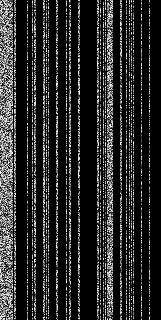
\includegraphics[width=2cm]{log-abs-data}
	\caption[Running example: Zero-filled data]{%
		The logarithm of the absolute value of the zero filled data \( \Adjoint{\Mask}\Data \).
	}%
	\label{fig:running example data}
\end{sidefigure}
\Cref{fig:running example reference-rss} and~\cref{fig:running example data} depict the reference signal and the data respectively.
In order to visualize the data \( y \), we map it back to \( \C^{\Height \times (\lfloor \Width / \num{2} \rfloor + \num{1})} \) using \( \Adjoint{\Mask} \).

This chapter is dedicated to finding
\begin{equation}
	\argmin_{x \in \R^{\Height \times \Width}} \Half \norm{\Forward\Signal - \Data}_{\num{2}}^{\num{2}} + R(x)
	\label{eq:running example optimization problem}
\end{equation}
under varying choices of \( R \).
To underscore the significance of the choice of \( R \), we initially set \( R \equiv 0 \).
Consequently, the least squares problem \( \argmin_{x \in \R^{\Height \times \Width}} \{ f(x) \coloneqq \Half \norm{\Forward\Signal - \Data}^{\num{2}} \} \) has the (not necessarily unique) solution \( \Adjoint{\Forward}\Data \).
This can be seen by noting that Fermat's condition (\cref{th:fermat}) at \( \Adjoint{\Forward}\Data \),
\begin{equation}
	\Grad f(\Adjoint{\Forward} \Data) = \Adjoint{\Forward}(\Forward\Adjoint{\Forward}\Data - \Data) = 0,
\end{equation}
is fulfilled since \( \Forward\Adjoint{\Forward} = \Mask\Fourier_{\R}\Adjoint{\Fourier_{\R}}\Adjoint{\Mask} = \Identity \) (on \( \C^f \)).
This solution is commonly referred to as the \emph{zero-filling} solution, as \( \Adjoint{\Forward} y = \Adjoint{\Fourier_{\R}}\Adjoint{\Mask}y \) essentially fills the missing frequencies with \num{0} before inverting the Fourier transform.
The reconstruction in~\cref{fig:running example reconstructions/zero-filled} shows the classical back-folding artifacts as well as high-frequency noise.
\RunningExampleFigure{reconstructions/zero-filled}{Naive reconstruction}{Zero-filling solution \( \Adjoint{\Fourier_{\R}}\Adjoint{\Mask}y \).}

\section{Classical variational penalties}
As the first interesting choice for \( R \), we consider the quadratic two-norm \( \frac{\lambda}{2} \norm{}^{\num{2}} \), where \( \lambda > 0 \).
Under this choice of \( R \), the first order optimality conditions of~\cref{eq:running example optimization problem} lead to the unique solution
\begin{equation}
	\Optimal{\Signal} = (\Adjoint{\Forward} \Forward + \lambda\Identity)^{-1} \Adjoint{\Forward}\Data,
\end{equation}
where the existence of the inverse of the operator \( \Adjoint{\Forward} \Forward + \lambda \Identity \) is assured by construction.

This regularization is extremely popular in many applications;
for instance, in machine learning applications it is called \emph{weight decay}~\cite[section 5.2.2, section 7.1.1]{goodfellow_deeplearning_2016}.
In the Bayesian framework adopted in this thesis, it corresponds to the assumption that the underlying signal is normally distributed with mean zero.
In imaging applications, this is typically not useful as it biases the solution towards dark images.
It enforces \enquote{regularity} solely on the magnitude of pixel intensities, irrespective of their neighbourhood, making in invariant with respect to arbitrary permutations of the pixels.
This characteristic is undesirable for regularizers of images, which have inherent spatial ordering.
\RunningExampleFigure{reconstructions/quadratic-intensities}{Quadratic intensity penalization}{Reconstruction using quadratic pixel magnitude penalization.}

For our forward operator, the inverse of \( \Adjoint{\Forward} \Forward + \lambda \Identity \) can be calculated quickly by noting that \( (\Adjoint{\Fourier_{\R}}\Adjoint{\Mask} \Mask\Fourier_{\R} + \lambda \Identity)^{-1} = (\Adjoint{\Fourier_{\R}}\Adjoint{\Mask} \Mask\Fourier_{\R} + \lambda \Adjoint{\Fourier_{\R}} \Fourier_{\R})^{-1} = (\Adjoint{\Fourier_{\R}}(\Adjoint{\Mask} \Mask + \lambda \Identity)\Fourier_{\R})^{-1} = \Adjoint{\Fourier_{\R}}(\Adjoint{\Mask} \Mask + \lambda \Identity)^{-1}\Fourier_{\R} \) where \( \Adjoint{\Mask}\Mask \) is a diagonal operator containing only ones and zeros.
Therefore, we have
\begin{equation}
	\begin{aligned}
		\Optimal{\Signal} &= \Adjoint{\Fourier_{\R}}(\Adjoint{\Mask} \Mask + \lambda \Identity)^{-1}\Fourier_{\R} \Adjoint{\Fourier_{\R}}\Adjoint{\Mask}\Data \\
						  &= \Adjoint{\Fourier_{\R}}(\Adjoint{\Mask} \Mask + \lambda \Identity)^{-1}\Adjoint{\Mask}\Data \\
						  &= (\num{1} + \lambda)^{-1}\Adjoint{\Fourier_{\R}}\Adjoint{\Mask}y,
	\end{aligned}
\end{equation}
where the last equality holds since \( \Adjoint{\Mask}\Data \) is only non-zero in entries whose corresponding position in the diagonal operator \( \Adjoint{\Mask} \Mask + \lambda \Identity \) are \( 1 + \lambda \).
In other words, the reconstruction shown in~\cref{fig:running example reconstructions/quadratic-intensities} is just the zero-filling solution multiplied by \( (1 + \lambda)^{-1} \).

Instead of penalizing the magnitude of pixel intensities, a fruitful approach is to penalize\footnote{%
	The regularizers we consider in these sections generally penalize responses.
	Later in~\cref{sec:overcompleteness through convolution} we discuss regularizers where this is not necessarily true.
} responses to linear filters.
Regularizers of this type can in general be represented as
\begin{equation}
	x \mapsto \lambda \sum_{i,j=\num{1}}^{m,n} \sum_{k=\num{1}}^{\NumExperts} \Potential_k\bigl((K_k x)_{i,j}\bigr).
	\label{eq:ridge regularizers}
\end{equation}
Here, \( \map{K_{\num{1}}, K_{\num{2}}, \dotsc, K_{\NumExperts}}{\R^{\Height \times \Width}}{\R^{\Height \times \Width}} \) are convolution operators (\cref{ssec:convolutions}) and \( \map{\Potential_{\num{1}}, \Potential_{\num{2}}, \dotsc, \Potential_{\NumExperts}}{\R}{\R} \) are scalar functions.

In this thesis, we adopt the nomenclature from the \gls{mrf} literature, see e.g.~\cite{geman_stoch_84,RoBl09,zhu_minimax_1997,zhu_filters_1998}.
Each operator \( K_k \) is endowed with its own \emph{potential} \( \Potential_k \), which is applied to the \emph{filter responses}.
In terms of the statistical model where the regularizer is interpreted as the negative log-prior, the regularizer encodes a \emph{Gibbs distribution}~\cite[theorem 1 and the two preceding definitions]{zhu_filters_1998} with density
\begin{equation}
	x \mapsto Z(K_{\num{1}}, \Expert_{\num{1}}, K_{\num{2}},\Expert_{\num{2}}, \dotsc, K_\NumExperts,\Expert_\NumExperts)^{\num{-1}} \prod_{i,j=\num{1}}^{\Height, \Width} \prod_{k=\num{1}}^\NumExperts \Expert_k\bigl( (K_kx)_{i, j} \bigr).
\end{equation}
Here, analogous to the products-of-experts model from Hinton~\cite{hinton_training_2002}, the one-dimensional functions \( \map{\Expert_{\num{1}}, \Expert_{\num{2}}, \dotsc, \Expert_\NumExperts}{\R}{\R} \) are termed \emph{experts}.
Thus, the potential \( \Potential_k \) is related to the expert \( \Expert \) via \( \Potential_k = -\log \Expert_k \).
The gradient of the potential function is called the \emph{activation}.\footnote{This is borrowed from the neural network literature.}
\( Z \) is the \emph{partition function} such that the density is normalized.

A simple choice for the convolution operators is \( \map{K_{\num{1}} = \DiffOp_h, K_{\num{2}} = \DiffOp_v}{\R^{\Height \times \Width}}{\R^{\Height \times \Width}} \), where \( \DiffOp_h \) and \( \DiffOp_v \) are discretizations of horizontal and vertical image gradients, respectively.
A standard choice~\cite{chambolle_algorithm_2004,chambolle_primal_2010,chambolle_pock_2016_acta_numerica} for defining these operators is through forward finite differences with Neumann boundary conditions,
\begin{equation}
	\begin{aligned}
		(\DiffOp_v x)_{i, j} &= \begin{cases}
			x_{i + \num{1},j} - x_{i,j} & \text{if } \num{1} \leq i < \Height, \\
			0 & \text{else},
		\end{cases}\\
		(\DiffOp_h x)_{i, j} &= \begin{cases}
			x_{i,j + \num{1}} - x_{i,j} & \text{if } \num{1} \leq j < \Width, \\
			0 & \text{else}.
		\end{cases}
	\end{aligned}
\end{equation}
This choice is popular due to its simplicity but there exist many other discretizations.
However, the choice of discretization rarely matters in applications~\cite{chambolle_upwind_2011} and we adopt the forward finite differences scheme.
For ease of notation, we define a linear operator \( \map{D}{\R^{\Height \times \Width}}{\R^{\Height \times \Width \times \num{2}}} \) that summarizes the application of \( D_v \) and \( D_h \) via
\begin{equation}
	(\DiffOp x)_{i, j, \num{1}} = (\DiffOp_v x)_{i, j}\ \text{and}\ (\DiffOp x)_{i, j, \num{2}} = (\DiffOp_h x)_{i, j}.
\end{equation}

When the potentials are shared and chosen as \( \Potential_{\num{1}} = \Potential_{\num{2}} = (x \mapsto x^{\num{2}}/{\num{2}}) \), the resulting regularizer can be compactly written as
\begin{equation}
	x \mapsto \frac{\lambda}{2} \sum_{i,j=\num{1}}^{\Height,\Width} \sum_{k=\num{1}}^{\num{2}} \bigl( (\DiffOp x)_{i,j,k} \bigr)^{\num{2}} = \tfrac{\lambda}{2} \norm{Dx}_{\num{2}, \num{2}}^{\num{2}}.
	\label{eq:quadratic gradient penalization}
\end{equation}
Here, the subscript in the norm emphasizes that we take a two-norm over both the pixel- and gradient dimensions.
This regularizer encodes the assumption that image gradients have Gaussian marginal distributions.

The corresponding optimization problem
\begin{equation}
	\argmin_{\Signal \in \R^{\Height \times \Width}} \Half \norm{\Forward\Signal - \Data}_{\num{2}}^{\num{2}} + \tfrac{\lambda}{2}\norm{\DiffOp\Signal}_{\num{2},\num{2}}^{\num{2}}
\end{equation}
can again be solved in closed form as
\begin{equation}
	\Optimal{\Signal} = (\Adjoint{\Forward}\Forward + \lambda \Adjoint{\DiffOp}\DiffOp)^{-1}\Adjoint{\Forward}\Data.
\end{equation}
The operator \( \Adjoint{\Forward}\Forward + \lambda \Adjoint{\DiffOp}\DiffOp \) is invertible when \( \ker(\Forward) \cap \ker(\DiffOp) = \Set{0} \).
Without going into too much detail, this condition is fulfilled as long as \( \Mask \) captures the DC-component of the signal, since \( \ker(\DiffOp) = \Set{\text{constant signals in}\ \R^{\Height \times \Width}} \).
However, to avoid storing the operator in memory we utilize Nesterov's accelerated gradient method (\cref{alg:nesterovs accelerated gradient method}) to solve the optimization problem.
To ensure convergence, we choose the step size sequence \( \tau^k = (\num{1} + \lambda\norm{\DiffOp}^{\num{2}})^{-1} \) using \(\sqrt{\num{8}} \) as an upper bound for \( \norm{D} \) from~\cite{chambolle_algorithm_2004}.

In the resulting reconstruction in~\cref{fig:running example reconstructions/quadratic-gradients}, some back-folding artifacts are removed, and the image appears less noisy than previous reconstructions.
However, edges appear overly smooth and small details such as the blood vessels in the fat tissue are almost completely lost.
This is because the quadratic potentials poorly match the empirical marginal distributions of edges in natural images.
\RunningExampleFigure{reconstructions/quadratic-gradients}{Quadratic gradient penalization}{Reconstruction using quadratic gradient penalization.}

It has been known at least since 1999 that the empirical marginal distributions of edges in natural images are highly non-Gaussian~\cite{hua_statistics_1999}.
This is illustrated in~\cref{fig:edge histograms}, which shows the empirical negative log-histograms of edges in natural images.
\begin{sidefigure}
	\def\aaa{80}
	\def\bbb{30}
	\def\ccc{18}
	\centering
	\begin{tikzpicture}
        \begin{axis}[
			height=4.6cm,
			width=4.6cm,
			xmin=-0.4,
			xmax=0.4,
			no markers,
			grid=major,
			table/col sep=comma,
			marginlabels,
        ]
			\addplot [maincolor, thick] table{./chapters/regularizers/scripts/edge-statistics/d_h.csv};
			\addplot [samples=100, domain=-.4:.4, dashed, thick] {\aaa*pow(x, 2) - 16.0};
			\addplot [samples=100, domain=-.4:.4, thick] {\bbb*abs(x) - 16.0};
		  \end{axis}
	\end{tikzpicture}
	\caption[Histograms of edges in natural images and approximations with convex functions]{%
		\tikzexternaldisable
		Negative log-histogram of horizontal edges in natural images %
		\protect\tikz[baseline=-\the\dimexpr\fontdimen22\textfont2\relax]\protect\draw [maincolor, thick] (0,0) -- (.5, 0);. %
		The quadratic %
		\protect\tikz[baseline=-\the\dimexpr\fontdimen22\textfont2\relax]\protect\draw [dashed, thick] (0,0) -- (.5, 0);, and absolute potentials %
		\protect\tikz[baseline=-\the\dimexpr\fontdimen22\textfont2\relax]\protect\draw [thick] (0,0) -- (.5, 0); %
		correspond to the choices in~\cref{eq:quadratic gradient penalization} and~\cref{eq:absolute gradient penalization} respectively.%
		\tikzexternalenable
	}%
	\label{fig:edge histograms}
\end{sidefigure}
These empirical marginal distributions are highly leptokurtic (\cref{def:excess kurtosis platykurtic mesokurtic leptokurtic}).
Huang and Mumford report an excess kurtosis of more than \num{14} in~\cite{hua_statistics_1999}.
Additionally, there is a very sharp peak at zero, indicating that the vast majority of edges in natural images are very close to zero.
Simultaneously, edges with large magnitude occur much more often than would be expected under a Gaussian distribution.
This \emph{sparsity} of edges in natural images is demonstrated in~\cref{fig:gradient sparsity of natural images}.
\begin{sidefigure}
	\centering
	\begin{tikzpicture}
		\begin{scope}
			\clip (-2, 2) -- (2, 2) -- (-2, -2) -- cycle;
			\node [anchor=center, rotate=180] at (0, 0) {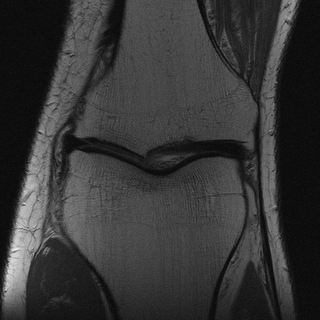
\includegraphics[width=4cm]{reference-rss}};
		\end{scope}
		\begin{scope}
			\clip (2, 2) -- (-2, -2) --(2, -2) -- cycle;
			\node [anchor=center, rotate=180] at (0, 0) {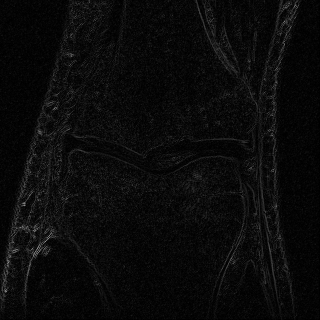
\includegraphics[width=4cm]{dx}};
		\end{scope}
	\end{tikzpicture}
	\caption[Sparsity of edges in natural images]{%
		Sum of the absolute horizontal and vertical difference of neighboring pixels (bottom right) of an \gls{mri} image from the fastMRI~\cite{zbontar_fastmri_2018} dataset (top left).
	}%
	\label{fig:gradient sparsity of natural images}
\end{sidefigure}

The analysis of the negative log-marginal distributions of edges in natural images (\cref{fig:edge histograms}) suggests considering other potential functions that match these more closely.
Among convex functions, the absolute value is best approximates the negative log-marginal distributions of edges.
Choosing \( \Potential_{\num{1}} = \Potential_{\num{2}} = \abs{} \) leads to the well known anisotropic \gls{tv} regularizer
\begin{equation}
	x \mapsto \lambda \sum_{i,j=\num{1}}^{m,n} \sum_{k=\num{1}}^{\num{2}} \abs*{(\DiffOp x)_{i,j,k}} = \lambda \norm{Dx}_{\num{1}, \num{1}}.
	\label{eq:absolute gradient penalization}
\end{equation}
Again, we adopt this simple interpretation of the discrete anisotropic \gls{tv} but point out that there exists a large literature on more elaborate, even learned (with respect to approximating some continuous energy), discretizations~\cite{bogensperger_learned_2023,chambolle_learning_2021,condat_tv_2017}.
Here, \emph{anisotropic} emphasizes that this regularizer favors grid-aligned edges.
We discuss different versions of the discrete \gls{tv} in~\cref{ssec:tv}.

The one-norm is a highly popular sparsity-inducing function~\cite{Daubechies2004,unser_representer_2016}.
There are many ways to see the sparsity-inducing property of the one-norm, such as the classical \enquote{intersection of level lines} in~\cite[figure 3.11]{Hastie2009} or by observing that its proximal map (\cref{def:proximal operator}) sets all elements smaller than a threshold to zero (see~\cref{fig:soft shrinkage}).
However, from the Bayesian perspective adopted in this thesis, the prior assumptions on the underlying signal are \emph{not} that \( Dx \) is sparse:
Although the \gls{map} solution favors sparse edges, samples from the Laplace distribution are never zero, e.g.\ see~\cite[fig. 1]{adler_deep_2018} for samples from a \gls{tv} prior.

This discrepancy is summarized by the difference between \emph{penalized likelihood estimation}, and \emph{Bayesian estimation}~\cite{bohra_phdthesis,gribonval_penalized_2011}.
In the former, the reconstructed signal has some abstract desirable regularity properties (like sparse edges), but the corresponding probabilistic model is in general \emph{not} a \enquote{good} model of the underlying distribution.
In the latter, the aim is to construct a good probabilistic model of the underlying distribution, whose corresponding \gls{map} estimate might not necessarily exhibit these abstract desirable regularity properties.
An illustrative example is~\cref{fig:gradient sparsity of natural images}: At almost all pixels, the sum of the absolute horizontal and vertical edges is almost zero.
Thus, we derive the abstract property that the underlying signal has sparse gradients.
However, a numerical check reveals that actually at exactly \emph{zero} pixels the sum of the absolute horizontal and vertical edges is \emph{exactly} zero.\footnote{%
	This has been checked on a \qty{32}{\bit} representation of the normalized image (maximum pixel intensity of \num{1}) with a threshold of \num{1e-7}.
	Only two pixels have a value lower than \num{1e-6}.
}
We refer to the papers of Gribonval et al.~\cite{gribonval_penalized_2011,gribonval_compressible_2012} for other Bayesian interpretations of penalized likelihood estimators and to the thesis of Bohra~\cite[section 2.2]{bohra_phdthesis} for a slightly more in-depth discussion.

Optimizing~\cref{eq:running example optimization problem} under the choice of \( R \) in~\cref{eq:absolute gradient penalization} is challenging because the absolute value is not differentiable.
This can be overcome by using differentiable surrogate functions such as \( x \mapsto \sqrt{x^{\num{2}} + \epsilon^{\num{2}}} \) or \( x \mapsto \epsilon^{-1}\log \cosh(\epsilon x) \) where \( \epsilon > \num{0} \)~\cite{chambolle_recovery_1997,charbonnier_deterministic_1997,charbonnier_deterministic_1994}.
The first choice was used by Charbonnier in 1994~\cite{charbonnier_deterministic_1994};
we use this differentiable surrogate in~\cref{chap:deep neural regularizers} for the isotropic \gls{tv} (see~\cref{ssec:tv}).
Another popular surrogate is the Huber function
\begin{equation}
	x \mapsto \begin{cases}
		x^{\num{2}} / \num{2} & \text{ if } \abs{x} \leq \epsilon, \\
		\epsilon(\abs{x} - \epsilon/\num{2}) & \text{ else},
	\end{cases}
\end{equation}
which we already introduced in~\cref{eq:huber function} as the Moreau envelope (\cref{def:moreau envelope}) of the absolute value.
\Cref{fig:absolute value and smooth variants} shows these surrogates for \( \epsilon = \num{1} \).
\begin{sidefigure}
	\begin{tikzpicture}
		\begin{axis}[%
			domain=-3:3,
			width=5cm,
			marginlabels,
			samples=200,
		]
			\addplot+{abs(x)};
			\addplot+{huber(x,1)};
			\addplot+{sqrt(pow(x, 2) + 1)};
			\addplot+{ln(cosh(x))};
		\end{axis}
	\end{tikzpicture}
	\caption[The absolute value and smooth surrogates]{%
		\tikzexternaldisable
		The absolute value %
		\protect\tikz[baseline=-\the\dimexpr\fontdimen22\textfont2\relax]\protect\draw [index of colormap={0} of flare, thick] (0,0) -- (.5, 0);
		and popular smooth surrogates:
		The Huber function %
		\protect\tikz[baseline=-\the\dimexpr\fontdimen22\textfont2\relax]\protect\draw [index of colormap={4} of flare, thick] (0,0) -- (.5, 0);,
		\( \sqrt{(\argm)^{\num{2}} + \num{1}} \) %
		\protect\tikz[baseline=-\the\dimexpr\fontdimen22\textfont2\relax]\protect\draw [index of colormap={8} of flare, thick] (0,0) -- (.5, 0);,
		and \( \log \circ \cosh \)
		\protect\tikz[baseline=-\the\dimexpr\fontdimen22\textfont2\relax]\protect\draw [index of colormap={12} of flare, thick] (0,0) -- (.5, 0);.
		\tikzexternalenable
	}%
	\label{fig:absolute value and smooth variants}
\end{sidefigure}

Using these approximations, we lose the interpretation of gradient \emph{sparsity}, since these functions are not sparsity-inducing (only \enquote{small value} inducing) and only approach the absolute value as \( \epsilon \) approaches zero.
As they approach the absolute value, the Lipschitz constant (\cref{def:lipschitz continuity}) of the their gradient necessarily has to explode.
This affects optimization algorithms since the step size (and hence the convergence speed) is bounded by the reciprocal of the Lipschitz constant of the gradient.

To achieve fast convergence even in the nondifferentiable case, we use primal-dual optimization algorithms.
Since the one-norm is a proper closed and convex function, it is equal to its biconjugate, see~\cref{th:biconjugate of convex function is itself}.
Thus, we can write
\begin{equation}
	\lambda \norm{x}_{\num{1},\num{1}} = (\Biconjugate{(\lambda\norm{}_{\num{1},\num{1}})})(x) = \max_{w \in \R^{\Height \times \Width \times \num{2}}} \inprod{w}{x} - (\ConvexConjugate{(\lambda \norm{}_{\num{1},\num{1}})})(w).
\end{equation}
The conjugate of the one-norm is the indicator function of the closed unit infinity-norm ball, see~\cref{th:convex conjugate of any norm}.
Additionally, we use~\cref{th:convex conjugate under postitive scaling} to identify
\begin{equation}
	\ConvexConjugate{(\lambda \norm{}_{\num{1},\num{1}})} = \lambda\IndicatorFunction{\Closure{\Ball{\norm{}_{\infty,\infty}}{\num{0}}{\num{1}}}}(\argm/\lambda) = \IndicatorFunction{\Closure{\Ball{\norm{}_{\infty,\infty}}{\num{0}}{\lambda}}},
\end{equation}
since indicator functions are invariant with respect to scaling and the scaling of the argument can be absorbed into the radius of the norm ball.
Thus,
\begin{equation}
	\lambda \norm{x}_{\num{1},\num{1}} = \max_{w \in \R^{\Height \times \Width \times \num{2}}} \inprod{w}{x} - \IndicatorFunction{\Closure{\Ball{\norm{}_{\infty,\infty}}{0}{\lambda}}}(w).
\end{equation}

The saddle point formulation of the optimization problem~\cref{eq:running example optimization problem} with the regularizer \( R \) being~\cref{eq:absolute gradient penalization} is
\begin{equation}
	\min_{\Signal \in \R^{\Height \times \Width}} \max_{w \in \R^{\Height \times \Width \times \num{2}}} \Half \norm{\Forward\Signal - \Data}_{\num{2}}^{\num{2}} + \inprod{w}{\DiffOp\Signal} +  \IndicatorFunction{\Closure{\Ball{\norm{}_{\infty,\infty}}{0}{\lambda}}}(w).
\end{equation}
This follows the structure~\cref{eq:primal dual saddle point structure} and we can use the \gls{pdhg} algorithm~(\cref{alg:pdhg},~\cite{chambolle_primal_2010}) to solve it efficiently.
In particular, the proximal map w.r.t.\ the indicator function is just a element-wise projection onto the interval \( \interval{-\lambda}{\lambda} \),
\begin{equation}
	w = \prox_{\IndicatorFunction{\Closure{\Ball{\norm{}_{\infty,\infty}}{0}{\lambda}}}}(\bar{w}) \iff w_{i,j,k} = \max(\min(\bar{w}_{i,j,k}, \lambda), -\lambda),
\end{equation}
and the proximal map w.r.t.\ the data fidelity term can be computed by
\begin{equation}
	\prox_{\tau\norm{\Forward\argm - \Data}_{\num{2}}^{\num{2}}/\num{2}}(x) = \Adjoint{\Fourier_{\R}}\bigl((\tau\Adjoint{\Mask}\Mask + \Identity)^{-1}(\Fourier_{\R} x + \tau\Adjoint{\Mask}\Data)\bigr).
	\label{eq:prox fourier data}
\end{equation}
There we used that \( \Adjoint{\Fourier_{\R}}\Fourier_{\R} = \Identity \) and note that \( \tau\Adjoint{\Mask}\Mask + \Identity \) is a diagonal operator that can be efficiently inverted.
In the algorithm, we used the standard choice \( \tau = \sigma = \frac{1}{\sqrt{8}} \).

The reconstruction in~\cref{fig:running example reconstructions/absolute-gradients} shows that back-folding artifacts are almost fully removed, the reconstruction has sharp edges, and some anatomical details are recovered.
\RunningExampleFigure{reconstructions/absolute-gradients}{Absolute gradient penalization}{Reconstruction using absolute gradient penalization, also known as the anisotropic total variation.}
However, it appears overly simplistic and fine anatomical structures such as the blood vessels in the fat tissue are almost entirely missing.
This simplification results from the simple model that only considers the distribution of differences between neighboring pixels and assumes these are independent random variables.

\Cref{fig:edge histograms} suggests nonconvex potential functions;
many have been proposed in the literature.
In \num{1985} Geman and McClure~\cite{geman_bayesian_1985} proposed the potential function
\begin{equation}
	x \mapsto -\bigl( \num{1} + (x / \gamma )^{\num{2}} \bigr)^{\num{-1}}
\end{equation}
where \( \gamma > \num{0} \) for photon emission tomography reconstruction.
Later, Huang and Mumford~\cite{hua_statistics_1999} considered the Student-t and generalized Laplace distributions.
The respective potential functions are
\begin{equation}
	x \mapsto \alpha \log \bigl( \num{1} + (x/\beta)^{\num{2}} \bigr)
\end{equation}
and
\begin{equation}
	x \mapsto \abs*{\frac{x}{\alpha}}^\beta
\end{equation}
where \( \alpha, \beta > \num{0} \) shape the potentials.
While these potentials better model the empirical marginal distributions of edges in natural images, the improvements over the absolute value are marginal.\footnote{;)}
\begin{sidefigure}
	\def\aaa{1.5}
	\def\bbb{0.01}
	\def\ccc{18}
	\centering
	\begin{tikzpicture}
		\begin{axis}[
			height=4.6cm,
			width=4.6cm,
			xmin=-0.4,
			xmax=0.4,
			no markers,
			grid=major,
			table/col sep=comma,
			marginlabels,
		]
			\addplot [maincolor, thick] table{./chapters/regularizers/scripts/edge-statistics/d_h.csv};
			\addplot [thick, samples=101, domain=-.4:.4] {\aaa * ln(1. + pow(x/\bbb, 2)) - 16};
			\addplot [thick, dashed, samples=101, domain=-.4:.4] {\ccc*sqrt(abs(x)) - 16};
		  \end{axis}
	\end{tikzpicture}
	\caption[Histograms of edges in natural images and approximations with nonconvex functions]{%
		\tikzexternaldisable
		The nonconvex Student-t %
		\protect\tikz[baseline=-\the\dimexpr\fontdimen22\textfont2\relax]\protect\draw [thick] (0,0) -- (.5, 0);
		and generalized Laplace potentials %
		\protect\tikz[baseline=-\the\dimexpr\fontdimen22\textfont2\relax]\protect\draw [dashed, thick] (0,0) -- (.5, 0);
		provide a good fit to the negative log-histograms of horizontal edges in natural images %
		\protect\tikz[baseline=-\the\dimexpr\fontdimen22\textfont2\relax]\protect\draw [maincolor, thick] (0,0) -- (.5, 0);.
		\tikzexternalenable
	}%
	\label{fig:edge histograms nonconvex functions}
\end{sidefigure}
\subsection{On the total variation}%
\label{ssec:tv}
In the previous section, we discussed \enquote{ridge-type} regularizers where a scalar potential function acts on filter responses and identified the discrete \emph{anisotropic} \gls{tv}
\begin{equation}
	x \mapsto \lambda \sum_{i,j=\num{1}}^{m,n} \sum_{k=\num{1}}^{\num{2}} \abs*{(\DiffOp x)_{i,j,k}} = \lambda \norm{Dx}_{\num{1}, \num{1}}
\end{equation}
as an instance of these models.
Here, isotropy is with respect to spatial directions, i.e.\ invariance with respect to rotations of the image.
Due to the definition of the forward finite difference operator \( \DiffOp \), this regularizer favors grid-aligned (horizontal and vertical) structures over oblique structures.
This anisotropy is essentially captured in~\cref{fig:norm balls}, where the one-norm ball is not radially symmetric.

To avoid these discretization artifacts, often the \emph{isotropic} \gls{tv}
\begin{equation}
	x \mapsto \lambda \sum_{i,j=\num{1}}^{m,n} \sqrt{\sum_{k=\num{1}}^{\num{2}} \bigl((\DiffOp x)_{i,j,k}\bigr)^{\num{2}}} = \lambda \norm{Dx}_{\num{2}, \num{1}}
\end{equation}
is employed.
There, the gradient \emph{magnitude} (as in the two-norm) is summed up over all pixels.
It turns out that the isotropic \gls{tv} is also anisotropic, see~\cite{condat_tv_2017}.
The isotropic \gls{tv} is not of the form~\cref{eq:ridge regularizers}, as the square root acts on the sum of the squares of the responses to two different filters, \( \DiffOp_v \) and \( \DiffOp_h \).
Thus, the isotropic \gls{tv} is in a more general class of regularizers.

The optimization of inverse problems with isotropic \gls{tv} regularization is usually performed with primal-dual methods similar to the anisotropic \gls{tv} discussed previously.
The associated saddle point problem problem is
\begin{equation}
	\min_{\Signal \in \R^{\Height \times \Width}} \max_{w \in \R^{\Height \times \Width \times \num{2}}} \Half\norm{\Forward\Signal - \Data}_{\num{2}}^{\num{2}} + \inprod{w}{\DiffOp\Signal} +  \IndicatorFunction{\Closure{\Ball{\norm{}_{\num{2},\infty}}{\num{0}}{\lambda}}}(w),
\end{equation}
which can be solved efficiently using \gls{pdhg} (\cref{alg:pdhg}).
The proximal map with respect to the indicator function is a pixel-wise projection onto two-norm balls with radius \( \lambda \),
\begin{equation}
	w = \prox_{\IndicatorFunction{\Closure{\Ball{\norm{}_{\num{2},\infty}}{\num{0}}{\lambda}}}}(\bar{w}) \iff w_{i,j} = \frac{\bar{w}_{i,j}}{\max(\num{1}, \norm{\bar{w}_{i,j}}_{\num{2}}/\lambda)}.
\end{equation}

\RunningExampleFigure{reconstructions/isotropic-tv}{Data-driven undercomplete regularizer}{%
	Reconstruction using the isotropic \gls{tv} regularizer (\qty{30.35}{\decibel}).
	The difference to the reconstruction obtained with anisotropic \gls{tv} (\cref{fig:running example reconstructions/absolute-gradients}) is almost negligible (\qty{30.32}{\decibel}).
}

For the image reconstruction problems considered in this thesis, the differences between the discretizations is largely irrelevant.
\Cref{fig:running example reconstructions/isotropic-tv} shows the reconstruction using the isotropic \gls{tv} which quantitatively improves the reconstruction from \qty{30.32}{\decibel} to \qty{30.35}{\decibel} in \gls{psnr} compared to the anisotropic \gls{tv}.
However, for more complex applications where the \gls{tv} is a building block, the choice of discretization can be crucial~\cite{chambolle_total_2018}.

In~\cref{chap:deep neural regularizers}, we require a smooth version of the \gls{tv} due to the structure of the optimization problems.
There, we use the isotropic \gls{tv} with the popular smoothing proposed by Charbonnier~\cite{charbonnier_deterministic_1994}.
In this case, the regularizer reads
\begin{equation}
	x \mapsto \lambda \sum_{i,j=\num{1}}^{m,n} \sqrt{\sum_{k=\num{1}}^{\num{2}} \bigl((\DiffOp x)_{i,j,k}\bigr)^{\num{2}} + \epsilon^{\num{2}}},
\end{equation}
where \( \epsilon > \num{0} \) controls the smoothness.
\section{Data-driven regularizers}
All regularizes discussed in the previous section were concerned with modeling the histograms of differences of neighboring pixels.
However, natural images are highly structured and the distribution of any pixel heavily depends on its neighbors.
Therefore, a good statistical model of images should take this structure into account.

Up to now, we have only considered first order forward finite difference filters with a receptive field of two pixels.
One way to account for the spatial structure in images is to use larger filters, where classical choices include derivative filters on different scales, Laplacian of Gaussian filters, and Gabor filters~\cite{zhu_prior_1997,zhu_filters_1998}.
However, it becomes increasingly difficult to choose the filters and model the potential functions manually.
A more feasible approach is to derive both the filters and the potential functions from data.
These types of models are called \emph{data-driven}.

The degree to which models of natural images are data-driven can vary greatly.
The regularizers discussed in the previous section are also in some sense data-driven:
We motivated different choices of potential functions via the empirical (\enquote{data-driven}) negative log-histogram of filter responses.
Generalizing this idea, we can derive the filters themselves within the framework described by
\begin{equation}
	x \mapsto \lambda \sum_{i,j=\num{1}}^{m,n} \sum_{k=\num{1}}^{\NumExperts} \Potential_k\bigl((K_k x)_{i,j}\bigr).
\end{equation}
To emphasize the image \emph{patches} in this formulation, we write this as
\begin{equation}
	x \mapsto \lambda \sum_{i, j=\num{1}}^{m, n} \sum_{k=\num{1}}^{\NumExperts} \Potential_k \bigl( \inprod{\Filter_k}{P_{i, j}x} \bigr).
	\label{eq:ridge regularizer 2}
\end{equation}
Here, the convolution operators \( K_{\num{1}}, K_{\num{2}}, \dotsc, K_\NumExperts \) implement the convolution with filters \( \Filter_{\num{1}}, \Filter_{\num{2}}, \dotsc, \Filter_\NumExperts \) of size \( b \times b \), and \( P_{i, j} \) extracts patches at pixel location \( (i, j) \) with appropriate boundary handling.
When treating overlapping patches as independent, it becomes evident that under the Bayesian interpretation that we adopt in this thesis, the above is a good model of the negative log-density of images when
\begin{equation}
	p \mapsto \lambda \sum_{k=\num{1}}^{\NumExperts} \Potential_k \bigl( \inprod{\Filter_k}{p} \bigr)
\end{equation}
is a good model of the negative log-density of image patches.
This independence assumption introduces a modeling error (except in the trivial case when \( b = \num{1} \)), which we address and resolve rigorously below.

A popular statistical model for image patches, which can be readily computed from a set of reference images, is given by the \gls{pca}~\cite{zoran_learning_2011}.
Following this idea, we plot the principal directions of all overlapping \( \numproduct{7x7} \) patches in the \num{300} images contained in the \gls{bsds}~\cite{martin_database_2001} training and validation data set\footnote{%
	We use the \gls{bsds} images here because they serve as training data in~\cref{chap:pogmdm}.
	The results would be similar for knee \glspl{mri}.
}
in~\cref{fig:pca of bsds patches}.
The principal directions associated with the largest singular value are low-frequency horizontal and vertical gradients.
As the singular value decreases, the filters obtain more and more high-frequency components.
Over all, the obtained filters closely resemble the basis images of the two-dimensional \gls{dct} and classical Gabor and Fourier filters.
For comparison, the basis images of the \gls{dct} are shown in~\cref{fig:discrete cosine transform basis}.
The observation that \gls{pca} of image patches recovers the \gls{dct} is related to the observation that the \gls{dct} is a good approximation of the Karhunen-Loève transform for stationary processes, as has been pointed out by Unser~\cite{unser_approximation_1984}.
\begin{figure*}
	\begin{tikzpicture}
		\csvreader[no head]{chapters/regularizers/scripts/pca/sigmas.txt}{1=\ssigma}{
			\pgfmathsetmacro{\component}{int(\thecsvrow-1)}
			\pgfmathsetmacro{\yy}{-int((\component)/12)*1.3}
			\pgfmathsetmacro{\xx}{mod((\component),12)*1.3}
			\node at (\xx, \yy-.65) {\tiny \( \num{\ssigma} \)};
			\node at (\xx, \yy) {\includegraphics[frame,width=1cm]{pca/directions/\component/d_\component}};
		}
		\draw [gray, thick, rounded corners] (-1.1cm, -4.8cm) rectangle (15.0cm, 0.7cm);
		\node at (-1.4cm, -2.05cm) [rotate=90] {Principal directions};
		\begin{scope}[xshift=-.5cm,yshift=-6.3cm]
			\begin{groupplot}[
				pogmdm group plot,
				group style={
					group size=12 by 4,
				},
				ymin=-17,
				ymax=-5,
				xmin=-.35,
				xmax=.35,
			]
				\pgfplotsforeachungrouped \component in {0, ..., 47}
				{
					\edef\tmp{%
						\noexpand\nextgroupplot%
						\noexpand\addplot [thick, maincolor] table[col sep=comma]{chapters/regularizers/scripts/pca/directions/\component/hist.csv};%
					}\tmp
				}
			\end{groupplot}
			\draw [gray, thick, rounded corners] (-0.6cm, -4.4cm) rectangle (15.5cm, 1.2cm);
			\node at (-0.9cm, -1.6cm) [rotate=90] {Empirical marginals};
		\end{scope}
	\end{tikzpicture}
	\caption[Principal directions of image patches]{%
		The principal directions of overlapping zero-mean patches extracted from natural images shown on top resemble the basis images of the \gls{dct} shown in~\cref{fig:discrete cosine transform basis}.
		The principal directions here are ordered by decreasing singular value shown below the directions; the last principal direction (which is the constant image) is omitted.
		On the bottom, the negative-log histogram of the filter responses is drawn.
	}%
	\label{fig:pca of bsds patches}
\end{figure*}
\begin{figure*}
	\begin{tikzpicture}
		\foreach \component in {0,...,48}
		{
			\pgfmathsetmacro{\yy}{-int((\component)/7)*1.2}
			\pgfmathsetmacro{\xx}{mod((\component),7)*1.2}
			\ifthenelse{\component=0}{}{\node at (\xx, \yy) {\includegraphics[frame,width=1cm]{dct/\component}};}
		}
	\end{tikzpicture}
	\caption[The basis images of the two-dimensional discrete cosine transform]{%
		The basis images of the two-dimensional \gls{dct}, in increasing horizontal frequency (left-to-right) and vertical frequency (top-to-bottom).
		The basis images are normalized such that they have a minimum and maximum of \num{-1} and \num{1} respectively; the first basis image (which is the constant image) is omitted.
	}%
	\label{fig:discrete cosine transform basis}
\end{figure*}

When the filters are aligned with the principal directions, it remains to detail the potential functions.
Since \gls{pca} provides an orthogonal basis, optimizing the potentials involves fitting each potentials to the corresponding observed negative log-marginal.
Using a suitable parametrization, such as piecewise constant functions~\cite{zhu_filters_1998} or radial basis functions~\cite{chen_trainable_2017}, this task becomes a least-squares fitting on the negative log-marginals.

The undercomplete model described in~\cref{chap:pogmdm} shares similarities these ideas, although the motivation is different.
This model also learns an orthogonal basis and parametrized potentials from a set of patches.
After training, the learned filters and potentials in~\cref{fig:learned patch reg} resemble the principal directions and negative log-marginals shown in~\cref{fig:pca of bsds patches}.
The negative log-marginals of the learned filters, shown in the bottom row of \cref{fig:learned patch reg}, closely match the learned potentials.
The shape of the learned negative log-marginals in \cref{fig:learned patch reg} remains consistent across all filters, while those of the principal directions in~\cref{fig:pca of bsds patches} appear \enquote{squashed} as the singular value decreases.
This difference is due to the choice of parametrization of the learned model where the filter norms change instead of the potentials being squashed.
The norm of the filters is related to the smallest and largest entry in the filter; these are shown below the filters in \cref{fig:learned patch reg}.
\begin{figure*}
	\centering
	\begin{tikzpicture}
		\csvreader[no head]{chapters/regularizers/scripts/ours/gmm/kvals.csv}{1=\kmin,2=\kmax}{
			\pgfmathsetmacro{\component}{int(\thecsvrow-1)}
			\pgfmathsetmacro{\yy}{-int((\component)/12)*1.3}
			\pgfmathsetmacro{\xx}{mod((\component),12)*1.3}
			\node at (\xx, \yy-.65) {\tiny \( \interval{\kmin}{\kmax} \)};
			\node at (\xx, \yy) {\includegraphics[frame,width=1cm]{ours/gmm/\component/k_\component}};
		}
		\draw [gray, thick, rounded corners] (-1.1cm, -4.8cm) rectangle (15.0cm, 0.7cm);
		\node at (-1.4cm, -2.05cm) [rotate=90] {Learned filters};
		\begin{scope}[xshift=-.5cm,yshift=-6.3cm]
			\begin{groupplot}[
				pogmdm group plot,
				group style={
					group size=12 by 4,
				},
				ymin=-3,
				ymax=8,
				xmin=-1,
				xmax=1,
				xticklabel=\empty,
			]
				\pgfplotsforeachungrouped \component in {0, ..., 47}
				{
					\edef\tmp{%
						\noexpand\nextgroupplot%
						\noexpand\addplot [thick, maincolor] table[col sep=comma, x=x, y=a]{chapters/regularizers/scripts/ours/gmm/\component/potentials.csv};%
					}\tmp
				}
			\end{groupplot}
			\draw [gray, thick, rounded corners] (-0.6cm, -4.1cm) rectangle (15.5cm, 1.2cm);
			\node at (-0.9cm, -1.6cm) [rotate=90] {Learned potentials};
		\end{scope}
		\begin{scope}[xshift=-.5cm,yshift=-11.9cm]
			\begin{groupplot}[
				pogmdm group plot,
				group style={
					group size=12 by 4,
				},
				ymin=-17,
				ymax=-5,
				xmin=-1,
				xmax=1,
			]
				\pgfplotsforeachungrouped \component in {0, ..., 47}
				{
					\edef\tmp{%
						\noexpand\nextgroupplot%
						\noexpand\addplot [thick, maincolor] table[col sep=comma,x=x,y=a]{chapters/regularizers/scripts/ours/gmm/\component/hists.csv};%
					}\tmp
				}
			\end{groupplot}
			\draw [gray, thick, rounded corners] (-0.6cm, -4.4cm) rectangle (15.5cm, 1.2cm);
			\node at (-0.9cm, -1.6cm) [rotate=90] {Empirical marginals};
		\end{scope}
	\end{tikzpicture}
	\caption[Learned directions and potential functions]{%
		A learned undercomplete model based on filter responses.
		The learned filters (top) share striking similarity to the \gls{pca} basis shown in~\cref{fig:pca of bsds patches}.
		The intervals below the filters show the value of black and white respectively.
		The learned potential functions (middle) match the negative-log empirical marginal distributions (bottom) almost perfectly.
		For more details, see~\cref{chap:pogmdm} and~\cite{zach_pogmdm_2024}.
	}%
	\label{fig:learned patch reg}
\end{figure*}

Due to the parametrization, the potential functions of this model are infinitely often differentiable but not convex, making the optimization problem~\cref{eq:running example optimization problem} smooth and non-convex.
Algorithms for solving these problems include \gls{ipiano} (see~\cref{alg:ipiano}) or non-convex \gls{fista} (see~\cref{alg:fista}).
We use the latter with a proximal step on the data fidelity which we recall from~\cref{eq:prox fourier data}, and determine the step sizes with backtracking~\cite{beck_fista_2009,ochs_ipiano_2014}.

The reconstruction using the learned regularizer\footnote{%
	The regularizer used to produce ~\cref{fig:running example reconstructions/patch-prior} is not exactly the one shown in~\cref{fig:learned patch reg}.
	Instead, to ease optimization we used the regularizer at diffusion time \( t = \num{5e-5}\), see~\cref{ssec:patch model}.%
} shown in~\cref{fig:running example reconstructions/patch-prior} appears more natural than the one using anisotropic \gls{tv} in \cref{fig:running example reconstructions/absolute-gradients}.
The back-folding artifacts are nearly eliminated and more details are retrieved without producing the staircasing artifacts associated with anisotropic \gls{tv}.
However, the reconstruction appears over-smoothed and important anatomical structures are missing.
In the next section, we discuss more expressive models that yield even better reconstructions.
\RunningExampleFigure{reconstructions/patch-prior}{Data-driven undercomplete regularizer}{Reconstruction using the undercomplete regularizer discussed in~\cref{chap:pogmdm}.}

\section{Overcomplete models and maximum entropy}%
\label{sec:overcompleteness through convolution}
In terms of the statistical model on the \emph{image}, the subtle but crucial assumption behind the previous models is the \emph{independence} of \emph{patches} at different pixel locations.
This introduces a modeling error, which we demonstrate with an example.
Consider three-by-three images where the marginal distribution of differences of neighboring pixels follow a normal distribution with unit variance.
Formally, let \( X \) be a random variable on \( \R^{\numproduct{3x3}} \) where
\begin{equation}
	(X_{i, j} - X_{i, j + \num{1}}) \sim \NormalDistribution_{\num{0},\num{1}}\ \text{for all}\ i = \numlist{1;2;3},\ \text{and}\ j=\numlist{1;2},
\end{equation}
and
\begin{equation}
	(X_{i, j} - X_{i + \num{1}, j}) \sim \NormalDistribution_{\num{0}, \num{1}}\ \text{for all}\ i = \numlist{1;2},\ \text{and}\ j=\numlist{1;2;3}.
\end{equation}
Using the approach from the previous sections where the density of \( X \) is modeled via the product of its marginals, we get
\begin{equation}
	\begin{aligned}
		&p_{\hat{X}}(x) \\
		&\propto \exp\Bigl( -\frac{(x_{\num{1},\num{1}} - x_{\num{1},\num{2}})^{\num{2}}}{\num{2}} \Bigr)\cdot\,\cdots\,\cdot\,\exp\Bigl( -\frac{(x_{\num{2},\num{3}} - x_{\num{3},\num{3}})^{\num{2}}}{\num{2}} \Bigr) \exp\Bigl( -\frac{\inprod{\num{1}}{x}^{\num{2}}}{\num{2}\sigma^{\num{2}}} \Bigr)\\
		&=\exp\Bigl( -\frac{\norm{\DiffOp x}_{\num{2},\num{2}}^{\num{2}}}{\num{2}} \Bigr)\exp\Bigl( -\frac{\inprod{1}{x}^{\num{2}}}{\num{2}\sigma^{\num{2}}} \Bigr).
	\end{aligned}
\end{equation}
Here, the density \( p_{\hat{X}} \) should match the density of \( X \).
The second tie-breaking factor ensures that \( p_{\hat{X}} \) is a density with respect to the Lebesgue measure on \( \R^{\numproduct{3x3}} \).\footnote{%
	It is needed such that the covariance matrix has full rank, but does not influence the main point of the discussion.
}
\( p_{\hat{X}} \) is the density of a normal distribution on \( \R^{\numproduct{3x3}} \) with covariance
\begin{equation}
	\bigl( \Adjoint{D}D + \frac{\num{1}\Adjoint{\num{1}}}{\sigma^{\num{2}}} \bigr)^{-1}.
\end{equation}
Through a linear change of variables, the random variable \( \DiffOp\hat{X} \) is normally distributed with mean \num{0} and covariance
\begin{equation}
	\DiffOp\bigl( \Adjoint{\DiffOp}\DiffOp + \frac{\num{1}\Adjoint{\num{1}}}{\sigma^{\num{2}}} \bigr)^{\num{-1}}\Adjoint{\DiffOp},
\end{equation}
see e.g.\ \cite[theorem 3.1]{Gut2009} for a proof.
The resulting random variables \( (D\hat{X})_{i, j, k} \) have different variances, with border edges having a variance of approximately \( \num{0.708} \), and edges involving the central pixel approximately \( \num{0.583} \), as illustrated in~\cref{fig:variances with prescribed marginals}.\footnote{%
	We were unable to come up with a general analytic expression for these numbers as a function of image size and pixel index;
	they were computed by inverting the covariance matrix.
}
The variance of the probabilistic tie-breaking factor, \( \sigma^{\num{2}} \), has no effect on these numbers.

In this example, prescribing Gaussian marginals led to observed Gaussian marginals in the product model due to closure properties of random variables with normal distributions, albeit with different and spatially dependent variances.
In the general non-Gaussian case the observed marginals are not necessarily from the same family of distributions.
For instance prescribing Laplacian marginals \( p_{\hat{X}}(x) \propto \exp\bigl( -\norm{\DiffOp x}_{\num{1},\num{1}} \bigr) \) through \gls{tv} regularization leads to observed marginals that do not have Laplacian distributions.
\begin{figure*}
	\begin{tikzpicture}[
		darkstyle/.style={circle,draw,fill=gray!40,minimum size=20},inner/.style={dashdotted, thick}, outer/.style={thick, maincolor}
	]
		\foreach \x in {1,...,3}{
			\foreach \y in {1,...,3}{
				\node [darkstyle] (\x\y) at (2*\x,-2*\y) {\( x_{\y,\x} \)};
			}
		}
		\foreach \ind in {12,23,32,21}
		{
			\draw [inner] (22) -- (\ind);
		}
		\foreach [count=\offsp from 2] \offs in {1,2}
		{
			\draw [outer] (1\offs) -- (1\offsp);
			\draw [outer] (\offs1) -- (\offsp1);

			\draw [outer] (3\offs) -- (3\offsp);
			\draw [outer] (\offs3) -- (\offsp3);
		}
		\begin{axis}[
			domain=-1:1,
			width=6cm,
			at={(8cm,-5.5cm)},
			legend style={at={(7.5cm, 2cm)}, draw=none},
			legend cell align={left}, 
			]
			\addplot[samples=100, thick] {x^2};
			\addplot[samples=100, outer] {x^2/0.708};
			\addplot[samples=100, inner] {x^2/0.583};
			\legend{$x\mapsto x^{\num{2}}$,$x\mapsto x^{\num{2}}/\num{0.708}$,$x\mapsto x^{\num{2}}/\num{0.583}$}
		\end{axis}
	\end{tikzpicture}
	\caption[%
		In overcomplete models, prescribing the empirical marginals leads to a modeling error%
	]{%
		In overcomplete models, prescribing the empirical marginals leads to a modeling error:
		When each edge is modeled with Gaussian potentials with unit variance, the variances in the resulting product model vary spatially, and none of them is one.
	}%
	\label{fig:variances with prescribed marginals}
\end{figure*}

The mismatch between the prescribed and observed marginals is due to loops in the graph structure of the three-by-three image.
Loops in this graph structure make the model \emph{overcomplete}, with more factors than variables.
However, any interesting models of the form~\cref{eq:ridge regularizers} need necessarily be overcomplete, since each convolution operator already contributes as many factors as there are variables.
Thus, when we wish to have an accurate model of the underlying density, we cannot simply prescribe the marginals.

In light of this discussion, previous regularizers should be viewed as \emph{penalized likelihood estimators}:
While they yield good quantitative results through the \gls{map} estimate, they are generally not accurate models of the negative log-prior.
\subsection{The correct way to think about marginals}%
\label{ssec:correct way to think about marginals}
The previous example illustrated that modeling a distribution's density as a product of its marginals leads to modeling errors.
How should we correctly approach marginals in general models?
We address this by framing the problem in the maximum-entropy framework, inspired by the seminal works of Zhu, Wu, and Mumford~\cite{zhu_filters_1998,zhu_minimax_1997}.
This derivation is similar to those found in~\cite[section 3.1]{wainwright_graphical_2008} and~\cite[section 12.1]{Cover2005}.

The setup is as follows:
We are given \( M \) samples \( x_{\num{1}}, x_{\num{2}}, \dotsc, x_M \) from an unknown distribution with density \( p_X \), which we wish to model.
Let
\begin{equation}
	\phi = \frac{1}{M} \sum_{i=\num{1}}^M s(x_i)
\end{equation}
represent the empirical moment of this distribution under the statistic \( s \).
Our goal is to find a distribution \( \hat{p}_X \) that is consistent with this empirical moment.
Among all possible distributions consistent with the empirical moment, the principle of maximum entropy (\cref{def:entropy}) selects the one with the highest entropy, leading to the optimization problem
\begin{equation}
    \begin{array}{ll}
		\max_{\hat{p}_X}   & \Entropy(\hat{p}_X) \\
		\mbox{s.t.} & \Expectation_{\hat{p}_X}[\num{1}] = \num{1} \\
					& \Expectation_{\hat{p}_X}[s] = \phi.
    \end{array}
    \label{eq:maxent}
\end{equation}
The Lagrangian of this problem is given by
\begin{equation}
	\mathcal{L}(\hat{p}_X, \theta_{\num{0}}, \theta) = \Entropy(\hat{p}_X) + \inprod{\theta_{\num{0}}}{\Expectation_{\hat{p}_X}[\num{1}] - \num{1}} + \inprod{\theta}{\Expectation_{\hat{p}_X}[s] - \phi}
\end{equation}
where \( \theta_{\num{0}} \) and \( \theta \) are the dual variables.
It follows from the optimality condition
\begin{equation}
	\Grad_{\num{1}} \mathcal{L}(\hat{p}_X, \theta_{\num{0}}, \theta) = -\log \hat{p}_X(x) - \num{1} + \theta_{\num{0}} + \inprod{\theta}{s(x)} = \num{0}
\end{equation}
for all \( x \), that
\begin{equation}
	\hat{p}_X(x) = \frac{\exp(\inprod{\theta}{s(x)})}{\exp(\num{1} - \theta_{\num{0}})}.
\end{equation}
Combining this with the optimality condition on \( \theta_{\num{0}} \)
\begin{equation}
	\begin{aligned}
		\nabla_{\num{2}} \mathcal{L}(\hat{p}_X, \theta_{\num{0}}, \theta) &= \Expectation_{\hat{p}_X}[\num{1}] - \num{1} = \int \hat{p}_{X}(x)\,\mathrm{d}x - \num{1}\\
																  &= \int \frac{\exp(\inprod{\theta}{s(x)})}{\exp(\num{1} - \theta_{\num{0}})}\,\mathrm{d}x - \num{1} \\
														  &= \num{0}
	\end{aligned}
\end{equation}
implies that \( \hat{p}_X \) is an exponential family distribution with normalization constant \( Z(\theta) = \exp(\num{1} - \theta_{\num{0}}) \).

Thus, the canonical parameters \( \theta \) of the exponential family \( \hat{p}_X \) are the \emph{dual variables} in the maximum entropy problem~\eqref{eq:maxent} ensuring the moment matching condition
\begin{equation}
	\Expectation_{\hat{p}_X}[s] = \phi.
\end{equation}
Hence, the potential functions should not model the negative log-marginal distributions.
Instead, potential functions should be chosen such that \emph{samples from the model reproduce the marginal distributions observed in the reference data}.

Fulfilling the moment matching condition is notoriously difficult for models of the form
\begin{equation}
	- \log \hat{p}_X(x) = \sum_{i,j=\num{1}}^{\Height, \Width} \sum_{k=\num{1}}^{\NumExperts} \Potential_k((K_k \Signal)_{i, j}) + Z(\phi_{\num{1}},\phi_{\num{2}},\dotsc,\phi_k, K_{\num{1}}, K_{\num{2}}, \dotsc, K_k).
\end{equation}
Typically, learning these models involves computationally expensive \gls{mcmc} algorithms to approximate the normalization constant \( Z \) ~\cite{RoBl09,zhu_prior_1997,zhu_minimax_1997,zhu_filters_1998}.
In contrast, \cref{chap:pogmdm} uses score matching and ideas from diffusion models to learn a model of this type.
Details are provided in~\cref{chap:pogmdm}; here we present the resulting model and key differences from previously discussed models.

The learned filters and potential functions of this overcomplete model are shown in~\cref{fig:learned overcomplete reg}.
In contrast to the potentials discussed previously, they have multiple local minima and sometimes zero is not in the set of local minimizers.
Thus, structures in the image can be enhanced under minimization of this regularizer.
\begin{figure*}
	\begin{tikzpicture}
		\csvreader[no head]{chapters/regularizers/scripts/shearlets/lamdas.csv}{1=\llambda}{
			\pgfmathsetmacro{\component}{int(\thecsvrow-1)}
			\pgfmathsetmacro{\yy}{-int(\component/10)*1.6}
			\pgfmathsetmacro{\xx}{mod(\component,10)*1.6}
			\node at (\xx, \yy-.8) {\tiny \( \llambda \)};
			\node at (\xx, \yy) {\includegraphics[frame,width=1.3cm]{shearlets/\component/k_\component}};
		}
		\draw [gray, thick, rounded corners] (-1.cm, -2.6cm) rectangle (15.4cm, 0.9cm);
		\node at (-1.3cm, -0.8cm) [rotate=90] {Learned filters};
		\begin{scope}[xshift=-.5cm,yshift=-4.3cm]
			\begin{groupplot}[
				pogmdm group plot,
				group style={
					group size=10 by 2,
				},
				width=1.3cm,
				height=1.3cm,
				ymin=-1.5,
				ymax=3,
				xmin=-0.45,
				xmax=0.45,
				xticklabel=\empty,
			]
				\pgfplotsforeachungrouped \component in {0, ..., 19}
				{
					\edef\tmp{%
						\noexpand\nextgroupplot%
						\noexpand\addplot [thick, maincolor] table[col sep=comma]{chapters/regularizers/scripts/shearlets/\component/potential.csv};%
					}\tmp
				}
			\end{groupplot}
			\draw [gray, thick, rounded corners] (-0.5cm, -1.8cm) rectangle (15.9cm, 1.5cm);
			\node at (-0.8cm, -0.15cm) [rotate=90] {Potentials};
		\end{scope}
		\begin{scope}[xshift=-.5cm,yshift=-7.8cm]
			\begin{groupplot}[
				pogmdm group plot,
				group style={
					group size=10 by 2,
				},
				width=1.3cm,
				height=1.3cm,
				ymin=-19,
				ymax=-6,
				xmin=-0.45,
				xmax=0.45,
			]
				\pgfplotsforeachungrouped \component in {0, ..., 19}
				{
					\edef\tmp{%
						\noexpand\nextgroupplot%
						\noexpand\addplot [thick, maincolor] table[col sep=comma]{chapters/regularizers/scripts/shearlets/\component/hist.csv};%
					}\tmp
				}
			\end{groupplot}
			\draw [gray, thick, rounded corners] (-0.5cm, -2.1cm) rectangle (15.9cm, 1.5cm);
			\node at (-0.8cm, -0.3cm) [rotate=90] {Empirical marginals};
		\end{scope}
	\end{tikzpicture}
	\caption[Learned directions and potential functions]{%
		The learned overcomplete model based on shearlet responses.
		The filters (top) are a shearlet system and do not resemble the \gls{pca}-like filters in the undercomplete model shown in~\cref{fig:learned patch reg}.
		The number below the filters are their associated weights by which their output is multiplied.
		The learned potential functions (middle) are distinctly different from the negative-log empirical marginal distributions (bottom).
		In particular, they have multiple local minima such that they can enhance certain structures.
		Sometimes (e.g.\ the second, third and fourth potential functions from the left) zero is not even in the set of minima.
		For more details, see~\cref{chap:pogmdm} and~\cite{zach_pogmdm_2024}.
	}%
	\label{fig:learned overcomplete reg}
\end{figure*}

With this regularizer, the \gls{map} inference problem remains smooth and nonconvex and we again resort to nonconvex \gls{fista} with proximal steps on the data term.
The resulting reconstruction shown in~\cref{fig:running example reconstructions/patch-prior}, appears sharper and recovers details such as the blood vessels in the fat tissue.
\RunningExampleFigure{reconstructions/conv-prior}{Data-driven overcomplete regularizer}{Reconstruction using the overcomplete regularizer discussed in~\cref{chap:pogmdm}.}

The distinction between modeling under- and overcomplete regularizers is well-known~\cite{chen_trainable_2017,romano_boosting_2017,zhu_filters_1998,zoran_learning_2011}.
Often, undercomplete models in this context are called \enquote{patch priors} or \enquote{patch-based priors}~\cite{zoran_learning_2011}.\footnote{%
	Patch distributions can also be modeled with overcomplete models but the challenges remain the same.
}
However, sometimes this distinction is overlooked, as is the case of Roth and Black's~\cite{RoBl09} Student-t potential function for their overcomplete model.

Theoretically, any probability density function is determined by \emph{all} its marginal distributions, see~\cite[theorem 2]{zhu_filters_1998}.\footnote{%
	Their theorem is essentially the Fourier-slice theorem, which is closely related to tomography.
}
Thus, models of the form~\cref{eq:ridge regularizers} can represent arbitrary distributions.
However, this is only true for infinitely many (image-sized) filters.
This limitation motivates exploring more general function families.
In the next section, we introduce \emph{deep neural regularizers}, where the regularizer is encoded as a deep neural network.
\section{Deep neural regularizes}%
\label{sec:regularizers deep neural regularizers}
In this section, we depart from modeling probability densities trough structured models involving the product of one-dimensional experts and instead explore more general function classes.
Specifically, we consider functions \( N \) from \( \ImgDim \) to \( \R \) implemented by a \gls{nn}.
\Glspl{nn} are layered maps of the form
\begin{equation}
	N = L_l \composed L_{l-\num{1}} \composed \cdots \composed L_{\num{2}} \composed L_{\num{1}}
\end{equation}
where \( L_i \) is the \( i \)-th \emph{layer} (for \( i = \num{1}, \dotsc, l \)).
Each layer is a linear operator followed by a point-wise non-linearity;
detailed definitions can be found in~\cref{sec:neural networks}.
From this perspective, the regularizers in discussed previously can be viewed as one-layer networks where the linear operator is a convolution and the non-linearity is the potential function composed with the sum over all pixels.
In contrast to this, we now allow a cascade of functions to act on the features extracted in the first layer.
Training of the model is discussed in detail in \cref{chap:deep neural regularizers}.
Here, we assume a pre-trained model.

Unlike previous methods, deep neural regularizers cannot be easily inspected through filter and potential function visualization.
Although the first layer of the deep neural regularizer has a similar structure, it only becomes interpretable through considering the downstream cascade of functions.
Instead, we we visualize \emph{samples} drawn from the Gibbs distribution.
A good regularizer accurately models the negative log-prior if samples from its Gibbs distribution are indistinguishable from samples from the reference distribution.\footnote{
	In terms of~\cref{eq:maxent}, the statistic we aim to match is the delta distribution.
}
The deep neural regularizer we examine is tailored for MRI reconstruction of human knees, with the reference distribution being MRI scans from the fastMRI dataset.

To sample from the Gibbs distribution of the regularizer, we resort to \gls{mcmc} sampling, the details of which are discussed in~\cref{ssec:methods ml}.
In~\cref{fig:mri sampling}, the sampling trajectory describes a path from uniform noise to an image resembling a human knee \gls{mri}.
This confirms the regularizer prefers high-level structures present in the training data and that the regularizer is an accurate model of the negative log-prior.
\begin{figure*}
	\centering
	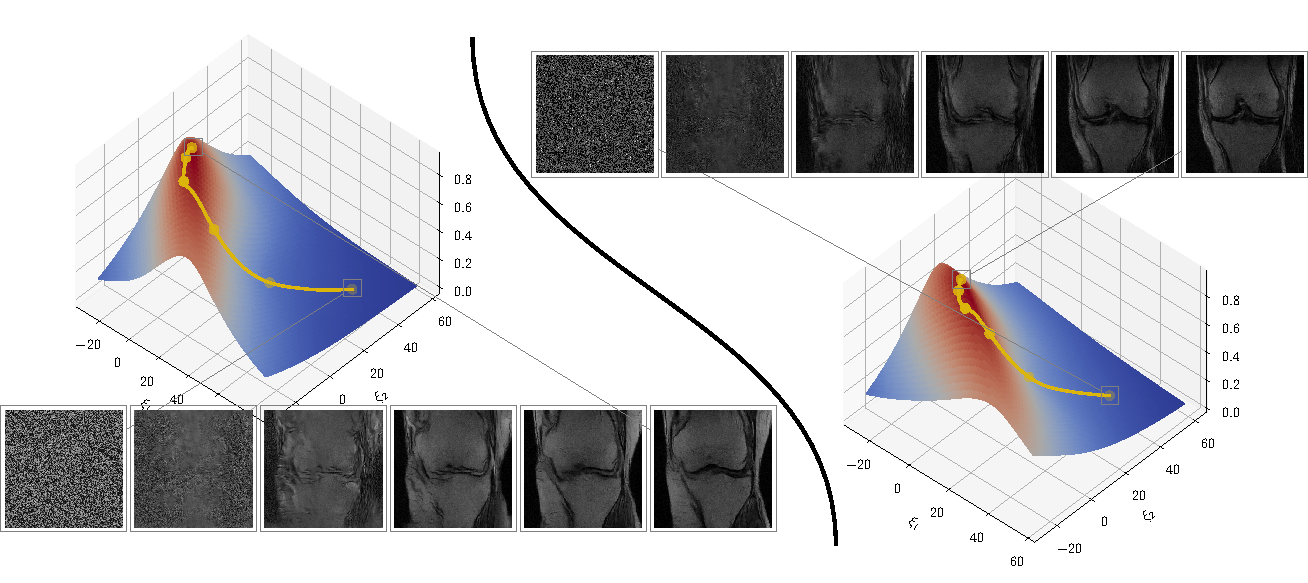
\includegraphics[width=\linewidth]{mri-sampling}
	\caption[Sampling a deep neural regularizer]{%
		We visualize preferred structures of the regularizer via \gls{mcmc} sampling.
		Uniform noise is unlikely under the deep neural regularizer whereas natural anatomical structures are very likely.
		The golden trajectory are the Langevin iterations; see the details in~\cref{ssec:data independent analysis}.
	}%
	\label{fig:mri sampling}
\end{figure*}

The \gls{map} inference problem with the deep neural regularizer is challenging.
The deep neural regularizer is not guaranteed to be convex\footnote{%
	This is somewhat of an understatement, it is almost surely not convex.
} and common neural network activation functions are not differentiable.
Traditional methods handle the non-differentiability is via proximal maps, but computing the proximal map with respect to the neural network is as hard as the original optimization problem, making this approach impractical.

Instead, we rely on nonconvex (nonsmooth) \gls{fista} for optimization, where the gradient step is replaced with a step on the Clarke subgradient (\cref{def:clarke subdifferential}) of the deep neural regularizer.
Specifically, at the point of nondifferentiability of the leaky rectified linear activation (\(\num{0}\)), we choose zero out of the subdifferential.
While we lack theoretical convergence guarantees, empirical results show fast convergence.

We observed that a good initialization is critical, which we achieve by running the optimization algorithm with a slightly noisy signal, matching the noise level used in Langevin iterations during training.see also~\cref{ssec:methods ml}.
Since accelerated algorithms can accumulate errors, we inject noise before gradient and function evaluation, not directly on the optimization variable.
After achieving suitable initialization, we proceed with standard algorithm.
In the resulting algorithm~\cref{alg:nonconvex fista with noise} we chose \( N_\eta = \num{1000} \), \( \gamma_{\num{1}} = \num{2} \), \( \gamma_{\num{2}} = \num{2}/\num{3} \).
After \( N_\eta \) iterations, the algorithm reduces to nonconvex nonsmooth \gls{fista}.
\begin{algorithm}
	\DontPrintSemicolon%
	\SetKwInOut{Input}{Input}
	\Input{Set \( L = \num{1} \), choose initial point \( x_{\num{0}} \in \ImgDim \), number of iterations with noise \( N_\eta \in \mathbb{N} \), noise level \( \epsilon > \num{0} \), backtracking multipliers \( \gamma_{\num{1}} \in \ointerval{1}{\infty}, \gamma_{\num{2}} \in \ointerval{\num{0}}{\num{1}} \).}
	\( x^{-1} = x^{\num{0}} \)\;
	\While{not converged}{
		\( \bar{x}^{k} = x^k + \frac{1}{\sqrt{2}} \bigl( x^k - x^{k-\num{1}} \bigr) \)\;
		\( \eta \sim \NormalDistribution_{\num{0}, \epsilon\Identity} \)\;
		\( \tilde{x}^k = \bar{x}^k + \CharacteristicFunction{\Set{1,\ldots,N_\eta}}(k) \eta \)\;
		\For{ever}{
			\( x^{k+\num{1}} = \prox_{L^{-1}h}\bigl(\bar{x}^k - L^{-1} \Grad g(\tilde{x}^k)\bigr) \)\;
			\uIf{\( g(x^{k+1} + \CharacteristicFunction{\Set{1,\ldots,N_\eta}}(k) \eta) < g(\tilde{x}^k) + \inprod{\Grad g(\tilde{x}^k)}{x^{k+\num{1}} - \bar{x}^k} + \frac{L}{2}\norm{x^{k+1} - \bar{x}^k}_{\num{2}}^{\num{2}}\)}{
				break\;
			}
			\( L = \gamma_{\num{1}}L \)\;
		}
		\( L = \gamma_{\num{2}}L \)\;
		\( k = k + \num{1} \)\;
	}
	\caption{Nonconvex nonsmooth noisy \gls{fista} with backtracking.}%
	\label{alg:nonconvex fista with noise}
\end{algorithm}

The resulting reconstruction shown in~\cref{fig:running example reconstructions/energy-based} is highly satisfactory.
Back-folding artifacts are entirely removed, small anatomical details such as the blood vessels in the fat tissue are restored well.
There are no obvious artifacts and the reconstruction looks natural over all.
In summary, the data-driven deep neural regularizer effectively captures the underlying distribution.
Samples drawn from its Gibbs distribution are almost indistinguishable from reference samples.
This carries over to inverse problem where the regularizer is able to restore anatomical features it has learned from the reference distribution.
Although without theoretical guarantees, the optimization of the deep neural regularizer is straightforward and the resulting images are artifact-free.
\RunningExampleFigure{reconstructions/energy-based}{Data-driven deep regularizer}{Reconstruction using the deep neural regularizer discussed in~\cref{chap:deep neural regularizers}.}

Combining the discussion on decision theory in \cref{chap:intro} with the Bayesian model, we expect that the \gls{mmse} will outperform the \gls{map} estimate.\footnote{At least quantitatively with respect to \gls{psnr}.}
For the sake of simplicity, we do not show \gls{mmse} estimates in this chapter, but quantitative results in~\cref{chap:deep neural regularizers} improve significantly from the \gls{map} estimate to the \gls{mmse} estimate.
\section{Conclusion}
In this section, we reviewed the historical development of regularizers.
Starting with classical methods such as quadratic penalization of gradients, we observed that fitting empirical statistics significantly improves the reconstructions in inverse problems.
The classical anisotropic \gls{tv} regularizer uses the absolute values as the best convex approximation to the empirical marginal distributions of pixel differences.
The nondifferentiability of the \gls{tv} motivated extensive research on nonsmooth optimization, exemplified by the development of the \gls{pdhg} algorithm~\cite{chambolle_primal_2010}.
Compared quadratic gradient penalization, these algorithms offer superior reconstruction quality.

The structure of the \gls{tv} can be viewed as a composition of \emph{prescribed} discrete gradient filters and absolute value potentials.
\emph{Data-driven} regularizers instead learn filters and potentials from a reference distribution.
For (under-)complete models on the space of patches, \gls{pca} provides a suitable filter basis and the optimal potentials can immediately be fit to the empirical marginal distributions.
This richer, data-fitting model outperforms classical TV regularization.

Extending an undercomplete model on image patches to images involves applying the learned filters as convolutions, resulting in an overcomplete model.
A common assumption for natural scenes is translation invariance of their statistics, implying that the potentials should be shared amongst all responses of an image on filter.
Even with shared potentials, the learning problem is significantly more complex.
However, once learned, the model captures richer statistics of the reference distribution.
Recently developed deep neural regularizers further elevate the reconstruction performance.

To conclude the chapter, we summarize the historical development of regularizers in~\cref{fig:running example comparison}.
Our best regularizer improves the naive reconstruction by \qty{5.16}{\decibel} in \gls{psnr}, and improves over anisotropic \gls{tv} regularization by \qty{2.78}{\decibel} in \gls{psnr}.
\begin{figure*}
	\begin{tikzpicture}
		\def\mywidth{4.2cm}
		\def\spywidth{2cm}
		\pgfmathsetlengthmacro{\myhpad}{2 * \spywidth + .8cm}
		\def\myvpad{0.8cm}
		\foreach [count=\imethod from 0] \method/\name/\psnr in {%
			reference-rss/{Reference}/\(\infty\),
			zero-filled/{\( R \equiv 0 \)}/27.94,
			quadratic-intensities/{\( x \mapsto \norm{x}^{\num{2}} \)}/26.76,
			quadratic-gradients/{\( x \mapsto \norm{\DiffOp x}_{\num{2},\num{2}}^{\num{2}} \)}/27.45,
			absolute-gradients/{\( x \mapsto \norm{\DiffOp x}_{\num{1},\num{1}} \)}/30.32,
			patch-prior/{\( x \mapsto \sum_{k=\num{1}}^\NumExperts \Potential_j(\inprod{\Filter_k}{x}) \)}/30.70,
			conv-prior/{\( x \mapsto \sum_{k=\num{1}}^\NumExperts \Potential_j(K_k x) \)}/30.93,
			energy-based/{\( x \mapsto R_\theta(x) \)}/33.10%
		}{%
			\pgfmathsetlengthmacro{\yy}{-abs(\imethod - 3.5) * (\mywidth + \myvpad)}
			\pgfmathsetlengthmacro{\xx}{int(\imethod / 4) * (\mywidth + \myhpad)}
			\pgfmathsetlengthmacro{\yyanno}{\yy - (\mywidth + \myvpad) / 2+0.05cm}
			\pgfmathsetlengthmacro{\xxspy}{\xx + pow(-1, (\imethod > 3)) * (\mywidth + 2cm) / 2}
			\pgfmathsetlengthmacro{\xxpath}{\xx + pow(-1, (\imethod < 4)) * 3cm}
			\ifthenelse{\imethod>0}{\fill (\xxpath, \yy) circle (0.2cm);}{}
			\pgfmathsetlengthmacro{\yypath}{\yy + or(\imethod==3,\imethod==4) * 3cm}
			\coordinate (path\imethod) at (\xxpath, \yypath);
			\begin{scope}[spy using outlines={rectangle, magnification=3, width=\spywidth, height=\mywidth}]
				\node at (\xx, \yy) {\includegraphics[width=\mywidth,angle=180]{reconstructions/\method}};
				\spy [maincolor] on (\xx + 1.5cm, \yy - .3cm) in node at (\xxspy, \yy);
			\end{scope}
			\ifthenelse{\imethod>0}{\node [rectangle, rounded corners, fill=white] at (\xx - 1.6cm, \yy + 1.8cm) {\psnr};}{}
			\node at (\xx, \yyanno) {\name};
		}
		\draw [thick, -latex] \foreach \x [remember=\x as \lastx (initially 1)] in {2,...,7}{(path\lastx) -- (path\x)} (path7) -- ++(0, -1);
	\end{tikzpicture}
	\caption[Running example: Comparison]{%
		The historical development of regularizers:
		\Glsxtrlong{tv} regularization improves over the naive reconstruction (\qty{27.94}{\decibel}) by \qty{2.38}{\decibel}, our best model improves over the \glsxtrlong{tv} regularization by \qty{2.78}{\decibel}.
	}%
	\label{fig:running example comparison}
\end{figure*}

\chapter{Deep neural regularizers}%
\label{chap:deep neural regularizers}%
\graphicspath{{chapters/deep-neural-regularizers/figures}}%
In \marginnote{\footnotesize \textbf{Contents:}\\\localtableofcontents}the previous chapter, we outlined the historical development of regularizers in imaging.
Starting from classical regularizers based on first principles, such as bounded norm or gradient sparsity of the signal, we highlighted the challenges of manually modeling image statistics and tuning parameters.
This led to the idea of \emph{learning} statistics from data.

In this chapter, we follow this idea by learning a generic deep neural regularizer that prefers structures present in the training data instead of prescribing any particular form of regularizer.
We design a \gls{nn} that maps from the input space, images of size \( \Height \times \Width \), to the real numbers and associate the output with a Gibbs distribution.
This Gibbs distribution is matched to the reference distribution by minimizing the Kullback-Leibler divergence (\cref{def:kullback leibler divergence}).
This chapter largely focuses on developing this idea in the context of \gls{mri} reconstruction, as some of our contributions are specific to this domain.
In particular, we propose a joint nonlinear inversion algorithm for parallel \gls{mri} that utilizes the data-driven regularizer.
However, we also present some results on \gls{ct} to demonstrate the approach's generality.

This chapter is structured as follows:
In~\cref{sec:intro deep neural regularizers} we give an overview of the problems encountered in \gls{mri} imaging and review data-driven reconstruction approaches.
In particular, we discuss approaches to parallel \gls{mri}.
\Cref{sec:discriminative pitfalls} highlights issues with discriminative approaches through a striking example and~\cref{sec:methods} outlines how we solve these problems through a generative approach.
This section encompasses discussion about the motivation behind the architecture of the deep neural regularizer, the probabilistic setup for parameter identification, and the fast joint nonlinear inversion algorithm.
The implementation details and practical considerations discussed in~\cref{ssec:details} are vital for reproducing the results and serve as a reference if anything remains unclear.
We show results on single-coil and multi-coil imaging in~\cref{sec:results deep neural regularizer}.
Additionally, this section focuses on interpretability of the results by visualizing the preferred structures of the regularizer in a data-independent analysis and through uncertainty quantification using the marginal posterior variance.
Further, we demonstrate that the regularizer remains stable when confronted with out-of-distribution data and that our joint nonlinear inversion algorithm yields superior coil sensitivities compared to offline estimation algorithms when few data are available.
Finally, in~\cref{sec:discussion} we discuss the implications and limitations of our approach and conclude that chapter in~\cref{sec:conclusion deep neural regularizer}.

This chapter is based on the following publications:\\
\rule{\linewidth}{.1em}
\fullcite{zach_computed_2021}\\[.2cm]
\fullcite{zach_stable_2023}\\
\rule{\linewidth}{.1em}
Code for training, validation, and visualization, along with pre-trained models, is available at \href{https://github.com/VLOGroup/stable-deep-mri}{https://github.com/VLOGroup/stable-deep-mri}.
A related publication, showing preliminary results of joint nonlinear inversion with diffusion priors, is~\cite{erlacher23}.
\section{Introduction}
\label{sec:intro deep neural regularizers}
\Gls{mri} is a crucial imaging techniques in clinical practice~\cite{Westbrook2018-pj}.
In \gls{mri}, a scanner's receiver coil measures the changes in magnetism of nuclei excited by radiofrequency pulses, and these measurements correspond to Fourier coefficients of the underlying signal via the two-dimensional discrete Fourier transform.
However, populating the observation with frequency data is time consuming and long examination times severely limit patient throughput.
Therefore, extensive research is dedicated to reducing examination time while retaining diagnostic value.

On the hardware side, parallel \gls{mri}~\cite{Roemer1990} exploits spatially varying sensitivities of coil arrays.
This has become standard in clinical systems, but noise amplification limits the potential speed up with classical reconstruction techniques~\cite{Robson2008}.
On the algorithmic side, compressed sensing~\cite{donoho_compressed_2006} and variational approaches enable greater acceleration.
As a prominent example, \gls{tv} regularization has been successfully applied to parallel \gls{mri}~\cite{Knoll2011}.

As shown in the previous chapter, variational approaches with classical penalties like \gls{tv} significantly improve reconstruction.
However, modern data-driven methods such as~\cite{akcakaya_raki_2019,chung_scoremri_2022,hammernik_learning_2017,Narnhofer2019,putzky_irim_2019,zbontar_fastmri_2018,zhou2020dudornet} now outperform these traditional methods.
Data-driven approaches have been applied successfully both as pre-processing steps in Fourier space~\cite{akcakaya_raki_2019} and as post-processing steps in image-space~\cite{zbontar_fastmri_2018}.
\Glspl{vn}~\cite{chen_tnrd_2017,cheng_pdnetworks_2019,hammernik_learning_2017,Kobler2017} unroll an optimization algorithm to imitate the iterative reconstruction schemes, while purely data-driven methods like AUTOMAP~\cite{zhu_image_2018} bypass physical measurement model entirely.

Despite their superior performance, data-driven approaches come with drawbacks that are especially relevant in the context of medical imaging.
First, these discriminative approaches act as a point estimators, mapping data directly to reconstructions.
In contrast, variational approaches enjoy a probabilistic interpretation through Bayes theorem, as discussed in~\cref{sec:variation methods and bayes theorem}.
Data are mapped to a \emph{distribution of reconstructions} which enables uncertainty quantification.
Second, point estimators are typically tied to a particular data likelihood, which is subject to change in \gls{mri} due to different frequency selections or anatomical features.
It has even been shown that reconstruction quality of some data-driven approaches deteriorates with increased data availability~\cite{Antun2020}.
We discuss similar findings in~\cref{sec:discriminative pitfalls}.
Third, these approaches typically rely on vast amounts of paired training data.
In the context of parallel \gls{mri}, this amounts to requiring fully-sampled frequency data which is extremely scarce.
\footnote{%
	The target can be computed from the fully-sampled data, and the input to the reconstruction algorithm can be created retrospectively.
}
In combination, these drawbacks severely hamper the adoption of these methods in clinical practice.

This chapter combines the strengths of modern data-driven methods with the benefits of classical variational approaches by learning a deep neural regularizer that serves as a plug-and-play replacement for classical variational penalties.
The accompanying probabilistic interpretation allows experts to explore the posterior distribution of any reconstruction problem.
We synthesizing realistic images \emph{without} any data, demonstrating that the regularizer encodes the negative log-prior faithfully.
Combining the data-driven regularizer with suitable data-likelihoods for different frequency selections achieves state-of-the-art performance.
Unlike most data-driven approaches, training our model only requires access to a database of reference reconstructions.\footnote{%
	Reference reconstructions are much more abundantly available than the corresponding fully sampled data, and constructing the data from the reconstructions is non-trivial.
}
In addition, we propose a joint nonlinear inversion algorithm based on \gls{ipalm}~\cite{pock_inertial_2016} for parallel \gls{mri}.
A sketch of our proposed approach is shown in~\cref{fig:reco}.
\begin{figure*}
	\centering
	\begin{tikzpicture}[>=latex]
		\def\kspacewidth{2cm}
		\def\kspacexoff{-1.8cm}
		\def\kspaceyoff{0.5cm}
		\def\kspacedx{0.25cm}
		\def\kspacedy{0.25cm}
		\def\sensewidth{0.7cm}
		\def\sensedx{0.1cm}
		\def\sensedy{0.1cm}
		\def\ppad{0.7cm}
		\def\prefix{examples-coils/01}
		\node [inner sep=0, outer sep=0] (kspace1) at (0 * \kspacedx + \kspacexoff, -1 * \kspacedy + \kspaceyoff) {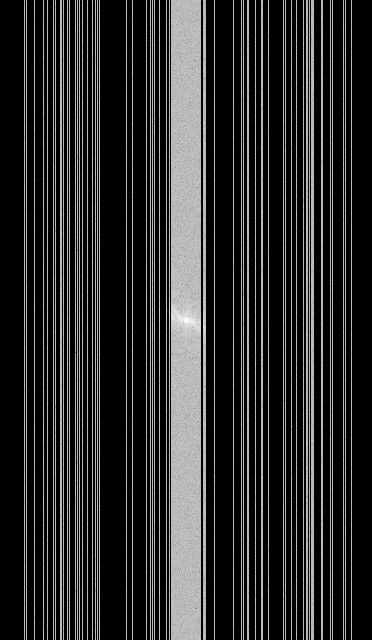
\includegraphics[width=\kspacewidth]{\prefix/kspace_masked/coil_00}};
		\node [inner sep=0, outer sep=0] (kspace2) at (1 * \kspacedx + \kspacexoff, -2 * \kspacedy + \kspaceyoff) {
\includegraphics[width=\kspacewidth]{\prefix/kspace_masked/coil_01}};
		\node [inner sep=0, outer sep=0] (kspace3) at (2 * \kspacedx + \kspacexoff, -3 * \kspacedy + \kspaceyoff) {
\includegraphics[width=\kspacewidth]{\prefix/kspace_masked/coil_02}};
		\node [inner sep=0, outer sep=0] (kspace6) at (5 * \kspacedx + \kspacexoff, -6 * \kspacedy + \kspaceyoff) {
\includegraphics[width=\kspacewidth]{\prefix/kspace_masked/coil_14}};

		\node [below left=-2mm of kspace1.south west] {\( \Adjoint{\Mask}\Data_{\num{1}} \)};
		\node [below left=-2mm of kspace6.south west] {\( \Adjoint{\Mask}\Data_c \)};
		\foreach \i in {1, 2, 3}
		{
			\pgfmathsetmacro{\fr}{\i/4}
			\node at ($(kspace3.south west)!\fr!(kspace6.south west)$) {\( \cdot \)};
			\node at ($(kspace3.north east)!\fr!(kspace6.north east)$) {\( \cdot \)};
		}
		\foreach [count=\i] \which in {00, 20, 40, 90}
		{
			\node[inner sep=0, outer sep=0] (reconstruction\i) at (1cm + \i * \kspacewidth + \i * \ppad, 0.3) {%
				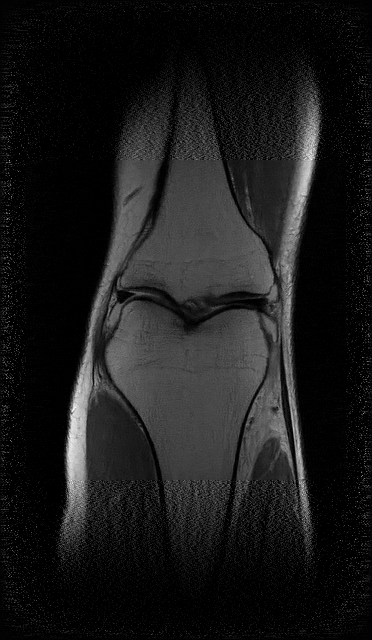
\includegraphics[angle=180,origin=c,width=\kspacewidth]{\prefix/0\which/reconstruction_unnormalized}%
			};
			\node at ($(reconstruction\i.north) + (0, 0.3cm)$) {%
				\ifthenelse{\i=1}{\( x^{0} \)}{%
					\ifthenelse{\i<4}{\( x^{\which} \)}{\( x^{K} \)}
				}%
			};
			\node at (1cm + \i * \kspacewidth + \i * \ppad, -2.5) {%
				\ifthenelse{\i=1}{\( \Sigma^{0} \)}{%
					\ifthenelse{\i<4}{\( \Sigma^{\which} \)}{\( \Sigma^{K} \)}
				}
			};
			\node at (0.9cm + \i * \kspacewidth + \i * \ppad, -1.95) {\( \ddots \)};
			\foreach [count=\isigma] \sigmawhich in {00, 01, 02, 14}
			{
				\ifthenelse{\isigma<4}{\def\offi{\isigma}}{\def\offi{6}}
				\node [inner sep=0, outer sep=0] (sensitivity maps\i\isigma) at (0.7cm + \i * \kspacewidth + \i * \ppad + \offi * \sensedx, -\offi * \sensedy - 1.0cm) {\includegraphics[width=\sensewidth]{\prefix/0\which/coil_\sigmawhich}};
			}
		}
		\node[rounded corners, rectangle, draw, minimum width=0.6cm, minimum height=0.6cm] (initial guess box) at ($(reconstruction1.west) + (-1.2, 0)$) {Naive};
		\draw [<-] (initial guess box) -- ++(-1, 0);
		\draw [->] (initial guess box) -- (reconstruction1);
		\draw [->] (initial guess box) |- (sensitivity maps14.west);
		\foreach \i in {1, 2, 3}
		{
			\pgfmathtruncatemacro{\j}{\i + 1}
			\node [inner sep=0,outer sep=0] (mid\i) at ($(reconstruction\i)!.5!(reconstruction\j)$) {\( \square \)};
			\draw (reconstruction\i) -- (mid\i) [-latex] -- (reconstruction\j);
			\draw [<-,dashed] (mid\i) -- ++(0, 1) node [above] {\( \Data \)};
		}

		\draw [rounded corners, ultra thick, draw=maincolor,] ($(reconstruction1.north west)+(-0.3, 0.6)$) rectangle ($(reconstruction4.south east) + (+0.3, -1.5)$);
		\begin{scope}[shift={(5, 7.5)}]
			\node (nablax) [draw, rounded corners] at (0, 0) {\( \bigl( \argm - L^{-1}_x \Grad H(\,\cdot\,, \Sigma^{k}) \bigr) \)};
			\draw [<-] (nablax) -- (nablax -| -3.8, 0) node [left] {\( x^{k} \)};
			\node (proxU) [draw, rounded corners] at (0, -1.1) {\( \max(0, \argm) \)};
			\draw [->] (proxU) -- (proxU -| 3.8, 0) node [right] {\( x^{k + 1} \)};

			\node (nablaS) [draw, rounded corners] at (0, -2.3) {\( \bigl( \argm - L^{-1}_\Sigma \Grad H(x^{k+1}, \argm)\bigr) \)};
			\draw [<-] (nablaS) -- (nablaS -| -3.8, 0) node [left] {\( \Sigma^{k} \)};
			\node (proxS) [draw, rounded corners] at (0, -3.5) {\( \Adjoint{\DiscreteSineTransform} \bigl( \DiscreteSineTransform(\mu\,\cdot\,) \oslash (\xi + \mu) \bigr) \)};
			\draw [->] (proxS) -- (proxS -| 3.8, 0) node [right] {\( \Sigma^{k + 1} \)};

			\draw [rounded corners, ultra thick, draw=black] ($(nablax.north west -| proxS.south west)+(-0.3, 0.3)$) rectangle ($(proxS.east |- proxS.south)+(0.3, -0.3)$);
			\draw [rounded corners, thick, draw=gray] ($(nablax.north west -| proxS.south west)+(-0.15, 0.15)$) rectangle ($(proxS.east |- proxU.south)+(0.15, -0.15)$);
			\draw [rounded corners, thick, draw=gray] ($(nablaS.north west -| proxS.west)+(-0.15, 0.15)$) rectangle ($(proxS.east |- proxS.south)+(0.15, -0.15)$);
			\draw [<-, dashed] (nablax.east) -- (3.2, 0) node [right] {\( \Data \)};
			\draw [<-, dashed] (nablaS.east) -- (3.2, 0 |- nablaS.east) node [right] {\( \Data \)};
			\draw [->] (nablax) -- (proxU);
			\draw [->] (nablaS) -- (proxS);
		\end{scope}
		\draw [dashed, opacity=0.5] (mid1.north west) to [in=-80,out=110] ($(proxS.south west)+(-0.3, -0.3)$);
		\draw [dashed, opacity=0.5] (mid1.north east) to [in=-110,out=80] ($(proxS.south east)+(0.3, -0.3)$);
	\end{tikzpicture}%
	\caption[Sketch of the joint nonlinear inversion algorithm for parallel MRI]{%
		Sketch of the reconstruction algorithm:
		To jointly reconstruct the spin density \( x \) and the coil sensitivities \( \Sigma = (\sigma_{\num{1}},\sigma_{\num{2}},\dotsc,\sigma_c) \), we impose data-fidelity, image-regularity, and coil-regularity in the iterations of \glsxtrshort{ipalm}~\cite{pock_inertial_2016}.
		The function \( H \) incorporates our data-driven regularizer acting on \( x \).
	}
	\label{fig:reco}
\end{figure*}

\subsection{Parallel MRI}
\label{ssec:parallel imaging intro}
Traditional \gls{mri} encodes the signal location by adjusting precession frequencies using gradient fields in spatial directions.
By exciting the nuclei with a radiofrequency pulse, the entry in the frequency plane encoded by the strength of the gradient fields could be filled.
The introduction of fast gradient-echo and spin-echo sequences, such as echo-planar imaging~\cite{Mansfield1977} or turbo spin-echo~\cite{Hennig1986}, allowed greater portions of the frequency plane to be filled with one excitation pulse.
To achieve even faster imaging, modern \gls{mri} systems employ coil arrays with spatially varying coil sensitivities, as pioneered by Roemer et al.~\cite{Roemer1990} in \num{1990}.
The spatially varying coil sensitivities can be exploited to reduce the number of required spatial modulations.

The following overview of reconstruction algorithms for parallel \gls{mri} draws from the review paper of Blaimer et al.~\cite{Blaimer2004}.
The conceptually simplest reconstruction algorithm for such data is \gls{pils} due to Griswold et al.~\cite{griswold_partially_2000}.
It assumes localized, non-overlapping coil sensitivities and that the entries in the frequency plane are such that the aliased coil images from undersampled reconstructions are non-overlapping.
The idealized situation for a Cartesian frequency selection with acceleration \num{2} is illustrated in~\cref{fig:pils}.
The idealized coil sensitivities of the two receiver coils each cover half of the image and the underlying signals can be recovered exactly.
\begin{figure*}
	\centering
	\begin{tikzpicture}[font=\footnotesize]
		\node at (0, 0) {
\includegraphics[frame, width=3cm]{../scripts/parallel-mri/s1}};
		\node at (0, -3.2) {
\includegraphics[frame, width=3cm]{../scripts/parallel-mri/s2}};
		\node at (0, -5) {Sensitivities};

		\node at (3.5, 0) {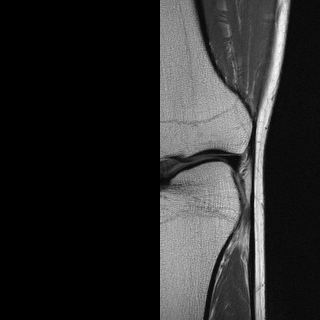
\includegraphics[frame, width=3cm]{../scripts/parallel-mri/ims1}};
		\node at (3.5, -3.2) {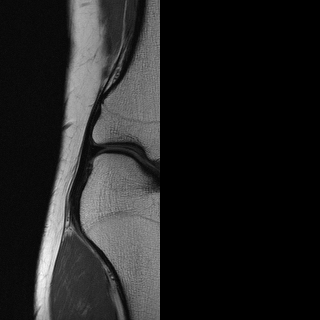
\includegraphics[frame, width=3cm]{../scripts/parallel-mri/ims2}};
		\node at (3.5, -5) {Coil images};

		\node at (7, 0) {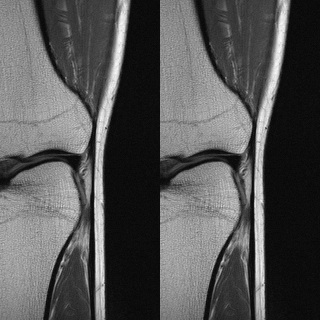
\includegraphics[frame, width=3cm]{../scripts/parallel-mri/image1}};
		\node at (7, -3.2) {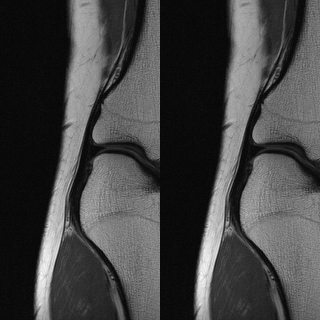
\includegraphics[frame, width=3cm]{../scripts/parallel-mri/image2}};
		\node at (7, -5) {Aliased reconstructions};

		\draw [maincolor, ultra thick] (7, 1.5) rectangle (8.5, -1.5);
		\draw [red!50!black, ultra thick] (7, -1.7) rectangle (5.5, -4.7);

		\begin{scope}[yshift=-1.6cm]
			\node at (10.5, 0) {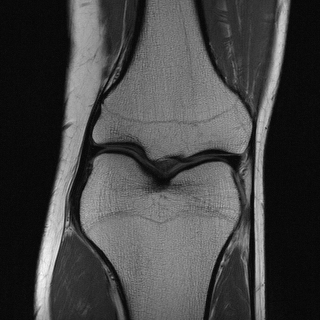
\includegraphics[frame, width=3cm]{../scripts/parallel-mri/reco}};
			\draw [maincolor, ultra thick] (10.5, 1.5) rectangle (12, -1.5);
			\draw [red!50!black, ultra thick] (10.5, 1.5) rectangle (9, -1.5);
			\draw [maincolor, ultra thick, dashed, dash phase=3pt] (10.5, 1.5) rectangle (12, -1.5);
			\draw [red!50!black, ultra thick, dashed] (10.5, 1.5) rectangle (9, -1.5);
			\node at (10.5, -1.8) {Reconstruction};
		\end{scope}
		\node at (14, -3.2) {
\includegraphics[frame, width=3cm]{../scripts/parallel-mri/mask}};
		\node at (14, -5) {Frequency selection};
		\node at (14, 0) {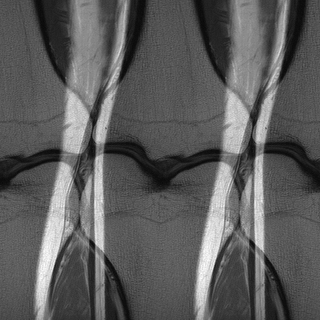
\includegraphics[frame, width=3cm]{../scripts/parallel-mri/aliased}};
		\node at (14, 1.8) {Naive reconstruction};
	\end{tikzpicture}
	\caption[The idea behind parallel imaging illustrated by an idealized example]{%
		The fundamental idea behind \gls{pils} algorithm~\cite{griswold_partially_2000} in an idealized case:
		The first column shows idealized coil sensitivities, each covering half of the measured area.
		The second column shows the underlying signal as seen by the coils; the third column are the per-coil naive reconstructions where the backfolding does not overlap the image.
		By taking the appropriate sections of each of the aliased coil images, the signal can be reconstructed exactly.
		On the right, the naive reconstruction with typical back-folding artifacts due to the frequency selection on the bottom is shown.
	}%
	\label{fig:pils}
\end{figure*}
However, the restriction to non-overlapping coil sensitivities and the required adaptation to the frequency selection renders the algorithm impractical.

The \gls{sense} algorithm due to Pruessmann et al.~\cite{pruessmann} extends this idea to arbitrary coil sensitivities and frequency selections.
Reconstructions are calculated by a linear weighting of the aliased coil images, where the weights are derived from the coil sensitivities.
Knowledge of the coil sensitivities necessitates a calibration scan in addition to the examination, and the speed-up is limited with classical linear reconstruction techniques due to noise amplification in regions where the sensitivities have significant overlap~\cite{Blaimer2004,pruessmann,Robson2008}.
The overlap is often characterized by the \enquote{geometry factor} or \( g \)-factor in the literature\cite{Robson2008}.

\Gls{pils} and \gls{sense} reconstruct the image from the aliased coil images.
In contrast to this are \gls{smash}~\cite{sodickson_simultaneous_1997} (more specifically, AUTO-SMASH~\cite{Jakob1998}) and \gls{grappa}~\cite{griswold_generalized_2002}.
These techniques reconstruct missing frequency data prior to Fourier inversion with the help of autocalibration data, which are typically low-frequency data in the center of the Fourier space.

In the intersection of these methods lies the popular ESPIRiT due to Uecker at al.~\cite{uecker_espirit_13}.
They demonstrated that coil sensitivities used in image domain approaches can be derived from autocalibration data used in frequency domain approaches.
Today, \gls{mri} reconstruction works typically use ESPIRiT to estimate coil sensitivities from autocalibration data~\cite{Aggarwal2019,darestani2021measuring,hammernik_learning_2017,jalal_robust_comporessed_2021,luo_bayesian_2023,zhu_image_2018}.
However, this explicit modeling of the coil sensitivities from autocalibration data has the drawbacks of prolonged scanning time and misalignment artifacts~\cite{Knoll2011,Ying2007}.
Additionally, most of the previous works assume a Cartesian frequency selection with measurements on a Cartesian grid,\footnote{%
	Acquiring frequencies off of the Cartesian grid is often called \emph{non-uniform} Fourier sampling.
} although radial, spiral or random sampling can be advantageous in different situations~\cite{lustid_compressed_2007,lustig2005faster,uecker_image_2008}.

To overcome the limitations of previous approaches, Bauer and Kannengiesser \cite{bauer_efficient_2007} propose to jointly estimate the image with the coil sensitivities.
Treating both as unknowns makes the reconstruction problem nonlinear; this is outlined later in~\cref{ssec:mri}.
We refer to the general principle as \emph{joint nonlinear inversion}.
They solve the joint nonlinear inversion using the iteratively regularized Gauss Newton method without any regularizers on the image or the coil sensitivities.
They treat the image and the coil sensitivities equally and do not resolve the ambiguity discussed in~\cref{ssec:mri} and consequently observe that the reconstruction is extremely sensitive to initialization, choice of regularization, and number of iterations of the algorithm.

Ying and Sheng independently proposed joint nonlinear inversion in~\cite{Ying2007} and resolve the ambiguity between the coil sensitivities and the image by observing that the coil sensitivities are \emph{much smoother than the image}.
They explicitly parametrize the coil sensitivities with low-order polynomials and solved the inversion using alternating minimization.
Uecker et al.~\cite{uecker_image_2008} built on this work but revisit the iteratively regularized Gauss Newton algorithm with smoothness of the coil sensitivities enforced through appropriate Sobolev norm penalties.
This approach was extended to include classic variational penalties on the image by Knoll et al.~\cite{Knoll2011} who report improved quantitative results using \gls{tv} and second-order \gls{tgv} regularization.

The work of Knoll et al.~\cite{Knoll2011} highlights the flexibility of formulating reconstruction as a nonlinear inverse problem.
Specifically, it accounts for smoothness penalties on coil sensitivities and sophisticated image regularization.
It is also not tied to Cartesian frequency selection and can account for nonuniform sampling.
However, their algorithm requires choosing multiple regularization parameters at each step and involves nontrivial subproblems to account for the variational penalties.

Our approach builds on the work of Knoll et al.~\cite{Knoll2011} but differs as follows:
Instead of handcrafted regularizers, we use modern generative learning techniques to learn an expressive regularizer from data, which leads to state-of-the-art reconstructions.
We enforce smoothness of the coil sensitivities quadratic gradient penalization gradient which simultaneously resolves ambiguities.
Instead of the iteratively regularized Gauss-Newton algorithm with non-trivial sub-problems, we employ the \gls{ipalm} algorithm~\cite{pock_inertial_2016} (\cref{alg:ipalm}) for optimization, ensuring convergence and requiring tuning of only two parameters (see~\cref{ssec:mri}).
Our reconstruction algorithm is sketched in~\cref{fig:reco} and takes about \qty{5}{\second} on consumer hardware.

For completeness, we mention that the end-to-end variational network of~\cite{sriram_endtoend_2020} also estimates the sensitivities jointly with the image.
However, their approach learns a mapping from frequency-space to image-space \emph{discriminatively}, using the estimated coil sensitivities to enforce data fidelity.
Thus, the network only works well with a particular frequency selection and coil configuration.
In contrast, we learn image features \emph{generatively} and impose handcrafted regularity onto the coil sensitivities.
\subsection{Related work}
\label{ssec:related work}
In this section we review related work on data-driven \gls{mri} reconstruction, focusing on methods similar to our proposed approach.
For a broader overview of data-driven \gls{mri} reconstruction, refer to~\cite{Zeng2021}.
Antun et al.~\cite{Antun2020} provide a comprehensive overview of the potential risks of using modern techniques for medical image reconstruction.

Guan at al.~\cite{Guan_energy_2022} explored learning a deep neural regularizer for \gls{mri} simultaneously to our work.
Unlike our approach but similar to the diffusion-based approaches discussed below, they apply their regularizer to the individual coil images in the reconstruction algorithm, requiring multiple evaluations of the gradient of the regularizer per iteration.
In addition, they estimate the sensitivity maps via ESPIRiT.\footnote{%
	Their exact reconstruction algorithm is unclear from their exposition.
}
In contrast, our joint nonlinear inversion algorithm eliminated the need for offline sensitivity estimation and requires only one gradient evaluation per iteration.

The authors extended their work in~\cite{tu_collaborative_2023} by learning an \gls{ebm} in image and frequency domain.
This eliminates the need for sensitivity estimation but requires training two independent networks that need to be balanced at inference time.
Additionally, the frequency-domain \gls{ebm} requires fully-sampled reference data, which is scarcely available.
Our method only requires reference DICOM (magnitude) images to train one regularizer.

Diffusion models are closely related to deep neural regularizers.
As discussed in~\cref{chap:pogmdm}, the score of a diffusion model \enquote{at time \num{0}} and the gradient of our regularizer model the same object:
The gradient of the negative log-prior.
Solving inverse problems with diffusion models is computationally demanding as it requires solving a \gls{sde} with high accuracy, typically requiring thousand of gradient evaluations~\cite{chung_scoremri_2022}.
Additionally, it is not clear how to optimally incorporate data-fidelity into the \gls{sde}.
Proposed solutions include data projection~\cite{song2022solving}, annealed Langevin dynamics~\cite{jalal_robust_comporessed_2021} and diffusion posterior sampling~\cite{chung2023diffusion}.
These methods require parameter tuning, in some cases at each step of the reverse diffusion~\cite{jalal_robust_comporessed_2021,chung2023diffusion}.
Feng at al.~\cite{feng2023scorebased} argue that none of these methods generate samples from the true posterior distribution and propose augmenting the score models with normalizing flows.
While their inference algorithm is parameter-free, the approach is opaque due to the introduction of the normalizing flow and is still computationally demanding.

Deep neural regularizers enjoy a natural probabilistic interpretation through Bayes theorem as discussed in~\cref{sec:variation methods and bayes theorem}.
\Gls{map} inference does not require solving an \gls{sde} and can be achieved by efficient through efficient optimization algorithms.
Access to the function value (not just the gradient) allows practical applications like inspecting the regularization landscape (see~\cref{fig:mri sampling}) and using backtracking in optimization algorithms~\cite{pock_inertial_2016}.%

Works by Luo et al.~\cite{luo_bayesian_2023} and Jalal et al.~\cite{jalal_robust_comporessed_2021} tackle parallel imaging by offline sensitivity estimation, which has drawbacks outlined in~\cref{ssec:parallel imaging intro}.
Chung et al.~\cite{chung_scoremri_2022} propose reconstructing individual coil images using a model trained solely on \gls{rss} reconstructions.
While the results are impressive, the computational cost depends on the number of coils and the authors report reconstruction times of up to \qty{10}{\minute}.
In our joint nonlinear inversion algorithm, the network's gradient is only evaluated once per iteration, regardless of the number of coils.
Imposing spatial regularity on the coils is extremely fast, requiring very few fast Fourier transforms at each iteration (see~\cref{ssec:mri}).

Finally, our generative approach has a practical benefit in the context of \gls{mri} reconstruction:
although we require \emph{reconstructions} from fully sampled data for training, it does not require fully sampled reference \emph{data}.
This distinction is important because reconstructions are more readily available in hospitals picture archiving and communication systems~\cite{zbontar_fastmri_2018}.
Constructing synthetic fully-sampled data from reference reconstructions is challenging due to the non-trivial interaction between coil sensitivities and the signal.
Most popular data-driven reconstruction algorithms like the end-to-end \gls{vn}~\cite{sriram_endtoend_2020}, AUTOMAP~\cite{zhu_image_2018}, and dual-domain approaches~\cite{tu_collaborative_2023,zhou2020dudornet} require image-data pairs for training.
Data-driven methods that need reference images include \glspl{gan}~\cite{Narnhofer2019}.
\Glspl{gan} suffer from the range-dilemma~\cite{bora_compressed_2017}, and authors have proposed to optimize the parameters of the \gls{gan} at inference time~\cite{Narnhofer2019}, effectively turning them into deep image priors~\cite{ulyanov_dip_2018}.
Deep image priors are challenging to optimize and don't offer a natural probabilistic interpretation.
\section{The pitfalls of discriminative signal recovery}%
\label{sec:discriminative pitfalls}
The classical way to utilizing deep learning methods in inverse problems involves learning a map from the data to the reconstruction \emph{discriminatively}.
However, this approach has significant drawbacks, particularly in medical imaging.
In this section we outline these drawbacks with a striking example.

The setup that we consider is as follows:\footnote{%
	We keep the setup general and don't specify any dimensionality or specific forward operator, \( A \), here.
}
We assume the signal to be reconstructed is an instance of a random variable \( X \) with density \( \DensityFunctionX \).
The data is summarized by a random variable related to the signals via
\begin{equation}
	Y = AX + N,
	\label{eq:relationship}
\end{equation}
where \( A \) is a linear operator with appropriate dimensions and \( N \) is Gaussian noise with known variance.
Thus, the signal and the data form a joint distribution \( p_{X\times Y} \) with the relationship between \( X \) and \( Y \) given by~\cref{eq:relationship}.

The discriminative approach in data-driven reconstruction methods involves a parametrized map \( f(\argm, \theta) \) that takes an instance of \( Y \) and outputs an estimation of \( X \).
The optimal parameters of the map are identified via the optimization problem
\begin{equation}
	\argmin_{\theta} \Expectation_{(X, Y) \sim p_{X\times Y}} \bigl[ l(f(Y, \theta), X) \bigr],
\end{equation}
where \( l \) is a loss function comparing the reconstruction \( f(y, \theta) \) with the reference signal \( x \).\footnote{Here, the lower case variables are instantiations of the corresponding random variables.}
Common loss functions include the negative \gls{ssim} (\cref{def:ssim}), and the two-norm or the one-norm of the difference.
This paradigm is extremely popular and includes pre-processing approaches~\cite{han_k-space_2020}, post-processing approaches~\cite{zbontar_fastmri_2018}, learned iterative networks~\cite{hammernik_learning_2017}, and AUTOMAP~\cite{zhu_image_2018}.

To emphasize the drawback of this approach, we consider the setup and baseline model from the original fastMRI publication~\cite{zbontar_fastmri_2018}.
Here, \( X \) is a random variable in \( \R^{\numproduct{320x320}} \) and \( \map{A = \Mask_{K}\Fourier}{\numproduct{320x320}}{\C^{\num{320}\times k}} \) is the Fourier transformation \( F \) followed by a Cartesian frequency selection, selecting \( k \in \mathbb{N} \) lines and \qty{8}{\percent} autocalibration lines, encoded in \( \Mask_{k} \);
this frequency selection operator is exemplified in the second column of~\cref{fig:simulation study masks}.
The map \( \map{f_k}{\C^{\num{320}\times k}}{\R^{\numproduct{320x320}}} \) is given by
\begin{equation}
	f_k(\argm, \theta) = \mathrm{UNet}(\argm, \theta) \circ \abs{} \circ \Adjoint{\Fourier}\Adjoint{\Mask_{k}}
\end{equation}
where \( \abs{} \) is the complex modulus acting element-wise on its argument and \( \mathrm{UNet}(\argm, \theta) : \R^{\numproduct{320x320}} \to \R^{\numproduct{320x320}} \) is a parametrized UNet.
This is a post-processing approach refining the zero-filling reconstruction with a learned UNet.
In the training, \( l \) is the one-norm and  \( k = \num{80} \) and the acceleration is \num{4}.

Let \( x \) be an image from the reference distribution, and let \( \Data_{k} = A_{k}x + n \) with n Gaussian noise.
\( k \in \mathbb{N} \) indicates the number of frequency lines that are available in the data.
For instance, when \( k = \num{320} \) the frequency space is completely filled.
\Cref{fig:unet kspace ablation} shows the \gls{psnr} of the reconstruction \( f_k(\Data_k, \theta) \) as \( k \) varies.
Notably, we observe that the \gls{psnr} decreases as \( k \) increases after around \( k = \num{140} \).
The reconstruction of the discriminative reconstruction network \emph{becomes worse as more data become available}.
\begin{figure*}
	\centering
	\begin{tikzpicture}[
		font=\footnotesize,
		rect annotation/.style={thick, fill, rectangle, inner sep=0.7mm},
	]
		\begin{axis}[
			xlabel={Available frequency lines},
			xticklabel={\pgfmathparse{\tick/320*100}\qty[round-mode=places,round-precision=0]{\pgfmathresult}{\percent}},
			ylabel={\gls{psnr} in \si{\decibel}},
			height=6cm, width=13cm,
			legend style={at={(1.06,.5)},anchor=west, draw=none},
			legend cell align={left},
		]
			\addplot [thick, black] table[col sep=comma, x=lines, y=naive]{chapters/deep-neural-regularizers/scripts/unet-kspace-ablation/psnr.csv};%
			\node (zero027) [rect annotation, black] at (axis cs:26, 22.26) {};
			\node (zero084) [rect annotation, black] at (axis cs:84, 22.96) {};
			\node (zero319) [rect annotation, black] at (axis cs:319, 46.14) {};

			\addplot [thick, red!50!black] table[col sep=comma, x=lines, y=unet]{chapters/deep-neural-regularizers/scripts/unet-kspace-ablation/psnr.csv};%
			\node (unet027) [rect annotation, red!50!black] at (axis cs:26, 25.63) {};
			\node (unet084) [rect annotation, red!50!black] at (axis cs:84, 32.02) {};
			\node (unet319) [rect annotation, red!50!black] at (axis cs:319, 29.03) {};

			\addplot [thick, maincolor] table[col sep=comma, x=lines, y=ours]{chapters/deep-neural-regularizers/scripts/unet-kspace-ablation/psnr.csv};%
			\node (ours027) [rect annotation, maincolor] at (axis cs:26, 25.44) {};
			\node (ours084) [rect annotation, maincolor] at (axis cs:84, 33.86) {};
			\node (ours319) [rect annotation, maincolor] at (axis cs:319, 46.67) {};
			\legend{Naive,Discriminative,Generative}
		\end{axis}
		\begin{scope}[xshift=1.5cm, yshift=-12.4cm]
			\foreach \offset/\kkappa in {0/027, 4.4/084, 8.8/319}
			{
				\node (\kkappa) [fill=maincolor, rectangle, inner sep=1mm] at (\offset-0.6, 0) {\includegraphics[rotate=180,width=4cm]{chapters/deep-neural-regularizers/scripts/unet-kspace-ablation/recos/ours/\kkappa}};
			}
		\end{scope}
		\begin{scope}[xshift=1.5cm, yshift=-8cm]
			\foreach \offset/\kkappa in {0/027, 4.4/084, 8.8/319}
			{
				\node (\kkappa) [fill=red!50!black, rectangle, inner sep=1mm] at (\offset-0.6, 0) {\includegraphics[rotate=180,width=4cm]{chapters/deep-neural-regularizers/scripts/unet-kspace-ablation/recos/unet/\kkappa}};
			}
			\node at (13.2-.7, 0) {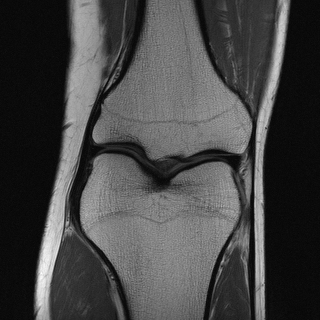
\includegraphics[rotate=180,width=4cm]{chapters/deep-neural-regularizers/scripts/unet-kspace-ablation/reference}};
			\node at (13.2-.6, 2.3) {Reference};
		\end{scope}
		\begin{scope}[xshift=1.5cm, yshift=-3.6cm]
			\foreach \offset/\kkappa in {0/027, 4.4/084, 8.8/319}
			{
				\node (\kkappa) [fill=black, rectangle, inner sep=1mm] at (\offset-0.6, 0) {\includegraphics[rotate=180,width=4cm]{chapters/deep-neural-regularizers/scripts/unet-kspace-ablation/recos/naive/\kkappa}};
				\draw [thick, black] (zero\kkappa.south) -- (\kkappa.north);
			}
		\end{scope}
	\end{tikzpicture}
	\caption[Discriminative signal recovery gets worse as more data becomes available]{%
		The signal recovered by the discriminative method deteriorates as more frequency lines become available:
		The reconstructions become overly sharp with accentuated details; when all data are available (\num{320} lines), the reconstruction is \qty{3.46}{\decibel} worse in \gls{psnr} than the reconstruction using \num{80} available frequency lines, which corresponds to the training setup.
		In contrast, due to the separation of likelihood and prior, the reconstruction of the generative approach improves with the availability of the data.
	}%
	\label{fig:unet kspace ablation}
\end{figure*}
\begin{sidefigure}
	\begin{tikzpicture}
		\node [inner sep=0, outer sep=0] at (0, 0) {\includegraphics[rotate=180,width=4cm]{chapters/deep-neural-regularizers/scripts/unet-kspace-ablation/recos/radial}};
		\draw [white, -latex, ultra thick] (-.8, -1.3) -- ++(-.4, -.4);
	\end{tikzpicture}
	\caption[Reconstruction with radial frequency selection]{Reconstruction with radial frequency selection; the white arrow indicates obvious artifacts.}
	\label{fig:radial reco}
\end{sidefigure}
This is \emph{not} an out-of-distribution application of the reconstruction network:
The underlying signal \emph{is} drawn from the reference distribution \( \DensityFunctionX \), but we slightly change its relationship with the data \( \Data_k \).

While the decrease in \gls{psnr} is significant, the resulting reconstruction remains artifact-free when using Cartesian frequency selection.
However, switching to a radial frequency selection leads to reconstructions with obvious artifacts. 
The reconstruction in \cref{fig:radial reco} suggests that the network cannot distinguish between anatomical features and artifacts in the zero-filled reconstruction.
This issue can even occur with Cartesian frequency selection (see \cref{fig:simulation study}).

The major drawback of discriminative reconstruction methods is their performance deterioration when the acquisition operator changes, even when the underlying reference distribution remains unchanged.
This is due to the acquisition operator being integrated in the training setup, causing the learned components to entangle features of the reference data and characteristics of the acquisition operator.

Despite this drawback, data-driven reconstruction methods offer significant benefits when the data matches the training setup, outperforming hand-crafted regularizers.
In the remainder of this chapter, we explore how modern generative learning methods can be used to learn the reference distribution.
We adopt a Bayesian approach, separating the likelihood (which uses the acquisition operator) from the prior assumptions on the reference distribution.
We learn the latter using generative learning methods and utilize the learned model in a Bayesian variational reconstruction framework.
\section{Methods}%
\label{sec:methods}
In this section, we first detail the neural network architecture used as the regularizer.
Then, we discuss how the parameters of this regularizer can be learned from the reference distribution.
To use the regularizer in a joint nonlinear inversion framework, we derive an algorithm based on \gls{ipalm} that enforces nonnegativity of the spin density and spatial regularity of the coil sensitivities.
\subsection{Network architecture}%
\label{ssec:network architecture}
Typical regularizers used in imaging applications are of the ridge-type, as defined in~\cref{eq:ridge regularizers}.
These regularizers apply potentials to the responses of linear filters, summing over all filters and pixels.
This structure makes the regularizers translation invariant, which is desired in natural image reconstruction where the probability of a feature is independent of the spatial location.\footnote{This class of images is often referred to as texture-like.}
However, this is not the case for for the highly structures \gls{mri} images of the human knee where specific structures like vertically aligned bones surrounded by muscle- and fat tissue are expected.
In addition, these types of images usually come with nonlocal dependencies:
If a large amount of fat tissue is observed medially from the bone, usually a large amount of fat tissue is present laterally, see the example in \cref{fig:translation invariance}.
Classical regularizes are limited in their ability to resolve these large scale dependencies.

Ridge-type regularizers are also often preferred due to their interpretability:
Filters and corresponding potentials can be visualized, showing experts which structures are enhanced or diminished.
The architecture that we will now describe can not be interpreted in this way.
However, in~\cref{ssec:data independent analysis} we will provide an alternative way of visualizing preferred structures by means of drawing samples from the Gibbs distribution.
\begin{figure*}
	\begin{tikzpicture}
		\foreach [count=\imc] \impath/\annotation in {texture-gray/Texture, natural/Natural image, knee-mri/Knee \gls{mri}}
		{
			\node at (5.5*\imc, 0) {\includegraphics[width=5cm]{translation-invariance/\impath}};
			\draw [thick, maincolor] (5.5*\imc-2, 1.2) rectangle ++(1, 1) node [below right, maincolor] {\Large 1};
			\draw [thick, maincolor] (5.5*\imc+1, -1) rectangle ++(1, 1) node [below right, maincolor] {\Large 2};
			\node at (5.5*\imc, 2.8) {\annotation};
		}
	\end{tikzpicture}
	\caption[Translation (in-)variance and (non-)local dependencies in images]{%
		\tikzexternaldisable%
		Translation (in)variance and (non)local dependencies in images:
		In the texture-like image on the left (\texttt{matted\textunderscore{}0166.jpg} from the describable textures dataset~\cite{cimpoi14describing}), the probability of a feature does not depend on the spatial location.
		This is also a common assumption for natural images as the one in the middle (\texttt{103070.jpg} from \gls{bsds}~\cite{martin_database_2001}), since the image we see is a (more or less) arbitrary crop of the infinitely extending scene.
		On the contrary, for the knee image on the right (the central slice of \texttt{file1001057.h5} from the fastMRI knee dataset~\cite{zbontar_fastmri_2018}), we always see the femur on top of the tibia, which are both surrounded by muscle- and fat tissue.
		In addition, knee \gls{mri} images carry nonlocal dependencies:
		Since there is very little fat tissue medially (e.g.\ %
			\protect\tikz[baseline=-\the\dimexpr\fontdimen22\textfont2\relax]\protect\draw [thick, maincolor] (-.15, -.15) rectangle ++(.3, .3) node [below right, maincolor] {1};%
		), we also expect very little fat tissue laterally (e.g.\ %
			\protect\tikz[baseline=-\the\dimexpr\fontdimen22\textfont2\relax]\protect\draw [thick, maincolor] (-.15, -.15) rectangle ++(.3, .3) node [below right, maincolor] {2};%
		).
		\tikzexternalenable%
	}%
	\label{fig:translation invariance}
\end{figure*}

In this chapter, we depart from the ridge-type architecture, opting for a more general architecture that is \emph{not} translation invariant and \emph{can} resolve nonlocal dependencies.
We model the regularizer \( \map{R(\argm, \theta)}{\ImgDim}{\R} \) as a cascade of convolutional layers with leaky rectified linear unit activation functions.
The parameters \( \theta \) of the regularizer are made explicit in the second argument; they are detailed below.

Formally, the regularizer has the structure
\begin{equation}
	R(\argm, \theta) = \abs{} \circ W_{l+\num{1}} \circ L_l \circ L_{l-\num{1}} \circ \ldots \circ L_{\num{2}} \circ L_{\num{1}}.
	\label{eq:deep neural regularizer architecture}
\end{equation}
All \( l \) layers \( L_{\num{1}}, L_{\num{2}}, \dotsc, L_l \) follow the structure
\begin{equation}
	\begin{aligned}
		\map{L_i}{\R^{n_i \times n_i \times c_i}&}{\R^{n_{i + \num{1}} \times n_{i + \num{1}} \times c_{i + \num{1}}}},\\
		x &\mapsto \relu(\widetilde{W}_i \relu(W_i x)).
	\end{aligned}
\end{equation}
Here, leaky rectified linear unit activation function \( \relu \colon x \mapsto \max\{ \gamma x, x \} \) is applied point-wise and has a leakage parameter \( \gamma > \num{0} \).
The linear operator \( \map{W_i}{\R^{n_i \times n_i \times c_{i}}}{\R^{n_i \times n_i \times c_{i}}} \) encodes\footnote{%
	In the special case \( i = \num{1} \), \( \map{W_{\num{1}}}{\ImgDim}{\R^{\Height \times \Width \times c_{\num{1}}}} \).
	\label{foot:special handling of first layer}
} a convolution with a \numproduct{3x3} kernel with zero-boundary conditions, while the linear operator \( \map{\widetilde{W}_i}{\R^{n_i \times n_i \times c_{i}}}{\R^{n_{i + \num{1}} \times n_{i + \num{1}} \times c_{i+\num{1}}}} \) encodes a \emph{strided} convolution with stride \num{2}, reducing the feature map dimensions progressively.
Thus, \( n_{i + \num{1}} = n_i / \num{2} \) and \( n_{\num{1}} = n \).\footnote{%
	In our setting, this always results in a natural number. We discuss the choice of the number of layers \( l \) and the progression of the number of channels \( c_i \) in the implementation details.
}
The final linear operator \( \map{W_{l+\num{1}}}{\R^{n_{l+\num{1}} \times n_{l + \num{1}} \times c_{l + \num{1}}}}{\R} \) is a dense, fully learnable layer that maps to a real number, essentially encoding a learned weighted sum.
Denoting with \( w_i \in \R^{\num{3} \times \num{3} \times c_i \times c_i} \) and \( \widetilde{w}_i \in \R^{\num{3} \times \num{3} \times c_i \times c_{i + \num{1}}} \) the learnable filters of the convolution operators \( W_i \) and \( \widetilde{W}_i \) respectively, the learnable parameters in our model are \( \theta = {\{ w_l, \widetilde{w}_l \}}_{i=\num{1}}^l \cup \{ W_{l+1} \} \).

Unlike ridge-type architectures where feature map responses are summed, our model progressively downsamples the feature maps via learned convolutions and nonlinearities until they are reduced to a scalar via a learned weighted sum.
This regularizer is not translation invariant and  it can prefer certain structures in certain regions, accommodation nonlocal structure arrangements.

The architecture of our regularizer can also be motived by considering its gradient with respect to the input image.\footnote{%
	The network is not differentiable; the gradient can be understood either via a differentiable surrogate of the rectified linear unit or in the sense of the Clarke subdifferential~\cref{def:clarke subdifferential}.
}
To derive the gradient, we note that \( L_i = \relu \circ \widetilde{W}_i \circ \relu \circ W_i \) and denote the \emph{activations} \( \relu^\prime \) of the point-wise activation functions after the convolution operators \( W_i \) and \( \widetilde{W}_i \) as
\begin{equation}
	a_i(x) = \bigl(\relu^\prime \circ W_i \circ L_{i-1} \circ \ldots \circ L_{\num{1}}\bigr)(x)
\end{equation}
and
\begin{equation}
	\tilde{a}_i(x) = \bigl(\relu^\prime \circ \widetilde{W}_i \circ \relu \circ W_i \circ L_{i-1} \circ \ldots \circ L_{\num{1}}\bigr)(x).
\end{equation}
We denote the activation of the final fully connected layer as
\begin{equation}
	a_{l + 1}(x) = \bigl( \abs{}^\prime \circ W_{l+1} \circ L_l \circ \ldots \circ L_{\num{1}} \bigr)(x).
\end{equation}
Then, by backpropagation
\begin{equation}
	\begin{aligned}
		&(\Grad R(\argm, \theta))(x) = \\
		&\Adjoint{W_{\num{1}}} \bigl( a_{\num{1}}(x) \cdot \Adjoint{\widetilde{W}_{\num{1}}} \bigl( \ldots \bigl( \tilde{a}_{l-1}(x) \cdot \Adjoint{W_l} \bigl( a_l(x) \cdot \Adjoint{\widetilde{W}_{l}}\bigl(\tilde{a}_l(x) \cdot \Adjoint{W_{l+1}} a_{l+1}(x) \bigr) \bigr) \bigr) \ldots \bigr) \bigr)
	\end{aligned}
\end{equation}
which has the structure of a UNet.

The UNet architecture, introduced by Ronneberger et al.\ in 2015~\cite{ronneberger_unet_2015}, has gained immense popularity in many applications requiring maps from the signal space to itself.\footnote{%
	The output space can also be \enquote{slightly different}. This is the case for instance in dense labeling or segmentation.
}
The key idea behind UNet is to capture context in the contracting path (via consecutive strided convolutions) and subsequently retrieve details in the expanding path (via consecutive adjoint strided convolutions).
To ensure detailed recovery in the expanding path and avoid loss of information, UNet employs \emph{skip connections} that retrieve features from the layers in the contracting path.
This is typically realized by concatenating the feature maps.

In modeling the gradient of a probability density, UNet-type architectures have become the standard backbone for diffusion models.\footnote{%
	We discuss diffusion models in more detail in~\cref{chap:pogmdm}. The relationship between our approach and diffusion models is covered superficially in~\cref{ssec:related work}
}
Works include the seed papers on diffusion models~\cite{song_generative_2019,song2021scorebased} and recent works that utilize diffusion models to solve inverse problems~\cite{chung_scoremri_2022,jalal_robust_comporessed_2021,chung2023solving,chung2023diffusion}.
A common criticism of these models (that we also make in this chapter and in~\cref{chap:pogmdm}) is that these networks are in general not a gradient.
This issue was noted in the paper on sliced score matching~\cite[footnote 1 on page 4]{song2020sliced}, a precursor to diffusion model papers, where the authors argued that the lack of gradient property does not significantly impact practical applications.

In contrast, our approach naturally retrieves a UNet-type model as the gradient of our scalar function.
The expanding path in each layer uses the adjoint operators of the corresponding contracting path layer.
The skip connections are realized by scalar multiplication of the feature maps in the expanding path by the activation from the contracting path.
This structure is schematically illustrated in~\cref{fig:deep neural regularizer architecture}.
\begin{figure*}
	\def\convcolor{rgb:blue,4;red,1;green,4;black,3}
	\def\skipcolor{rgb:blue,4;red,1;green,1;black,3}
	\def\FcColor{rgb:blue,5;red,2.5;white,5}
	\includegraphics[width=\linewidth]{network/gradient}
	\caption[Schematic of the gradient of the regularizer: A UNet]{%
		\tikzexternaldisable%
		The gradient of the regularizer has a UNet structure.
		At the \( i \)-th layer, the symbol %
			\protect\tikz[baseline=-\the\dimexpr\fontdimen22\textfont2\relax]\protect\draw [thick,draw=\convcolor, -Stealth] (0, 0) -- ++(.5, 0); %
		is the map \( x \mapsto \relu(\widetilde{W}_ix) \), and %
			\protect\tikz[baseline=-\the\dimexpr\fontdimen22\textfont2\relax]\protect\draw [thick,draw=\convcolor, -Stealth, dashed] (0, 0) -- ++(.5, 0); %
		is the map \( x \mapsto \Adjoint{\widetilde{W}_i}x \); the convolutions with unit stride are between the gray blocks and (for the sake of simplicity) are not endowed with an arrow.
		The skip connection
			\protect\tikz[baseline=-\the\dimexpr\fontdimen22\textfont2\relax]\protect\draw [thick,draw=\skipcolor, -Stealth] (0, 0) -- ++(.5, 0); %
		is understood as the map \( x \mapsto \relu^\prime(x) \), the result of which pointwise multiplies the features in the expanding path.
		The function value of the network is given as the absolute value of the scalar-valued feature map at the bottom, which is computed via the learned weighed sum (the fully connected layer \( W_{l+1} \)) %
			\protect\tikz[baseline=-\the\dimexpr\fontdimen22\textfont2\relax]\protect\draw [thick,draw=\FcColor, -Stealth, dashed] (0, 0) -- ++(.5, 0);.
		The annotations show the size of the feature maps.
		The illustration is slightly simplified; we neither explicitly show the nonstrided convolutions (these would be arrows between the adjacent blocks) nor their corresponding skip connections.
		\tikzexternalenable%
	}%
	\label{fig:deep neural regularizer architecture}
\end{figure*}

While our approach imposes some restrictions compared to a classical UNet, it accurately models the gradient of the log-prior, as empirically demonstrated in \cref{fig:mri sampling deep neural regularizers}.
Moreover, our model allows for the computation of function values, not just gradients, while preserving classical symmetry properties of gradients.
In the next section, we discuss how to learn the parameters of the regularizer such that is accurately models the negative log-prior.
\subsection{Parameter identification}%
\label{ssec:methods ml}
In the strict Bayesian view of inverse problems that we adopt in this thesis, we assume that in any reconstruction problem, the underlying signal is a realization of a random variable \( X \) with density \( \DensityFunctionX \).
In this chapter, the random variable has values in \( \ImgDim \) and represents the magnitude of \gls{mri} scans of the human knee, see the details in \cref{ssec:details}.
In this view, the regularizer in the inverse problem models the negative log-prior, up to an additive constant.

Under mild conditions we can associate any regularizer \( R(\argm,\theta) \) with a density
\begin{equation}
	\hat{\DensityFunction}_{\RandomVariable}(x) = \frac{\exp\bigl(-R(x,\theta)\bigr)}{\int_{\ImgDim}\exp\bigl(-R(\xi, \theta)\bigr)\,\mathrm{d}\xi}.
	\label{eq:gibbs}
\end{equation}
When \( R(\argm, \theta) \) is of ridge-type, then this construction is called a \emph{Gibbs distribution}, see~\cite[theorem 1 and the two preceding definitions]{zhu_filters_1998} and~\cite[page 5]{geman_stochastic_1984}.
Modern literature extend this to more general functions, including neural networks, which can also induce a Gibbs distribution via the equation above~\cite[section 3.1]{nijkamp_shortrun_2019},~\cite[section 2.1]{nijkamp_anatomy_2019}.

\( R(\argm, \theta) \) admits a Gibbs density if it is bounded from below and grows \enquote{fast enough} radially, such that \( \int_{\ImgDim}\exp\bigl(-R(\xi, \theta)\bigr)\,\mathrm{d}\xi < \infty \).
We ensure boundedness from below by using an absolute value activation in the last layer.
The growth condition can be achieved by adding a small quadratic term to the regularizer\footnote{%
	This is also a popular strategy to assign a proper distributions to ridge-type regularizers, see e.g.~\cite[eq. (1)]{schmidt_generative_2010} and~\cite[eq. (6)]{weiss_model_2007}.
} but in practice this is unnecessary.

Identifying the optimal parameters of the regularizer becomes a problem of density fitting, and we adopt the popular approach of minimizing the Kullback-Leibler divergence from \( \DensityFunctionX \) to \( \DensityFunctionXEstimation \).
The Kullback-Leibler divergence is popular due to the links to maximum likelihood and maximum entropy estimation.
Seminal papers that utilize it include~\cite{hinton_training_2002,RoBl09,zhu_filters_1998}; it has been called the \enquote{standard} divergence by Teh, Welling, Osindero and Hinton in~\cite{teh_energy_2003}.
The Kullback-Leibler divergence from \( \DensityFunctionX \) to \( \DensityFunctionXEstimation \) (see~\cref{def:kullback leibler divergence}) reads
\begin{equation}
	\KullbackLeibler{\DensityFunctionX}{\DensityFunctionXEstimation} = \int_{\ImgDim} \DensityFunctionX(x)\log\frac{\DensityFunctionX(x)}{\DensityFunctionXEstimation(x)}\,\mathrm{d}x.
	\label{eq:kullback leibler deep neural regularizers}
\end{equation}
As is common in the literature, we do not ensure that \( \DensityFunctionX \) is absolutely continuous (see~\cref{def:absolute continuity}) with respect to \( \DensityFunctionXEstimation \).
Even without guaranteeing this, we can \enquote{notationally} derive a learning objective that is useful in practice.

To derive the objective for parameter identification, we make the parametrization more explicit and write \( \DensityFunctionXEstimation \coloneqq \DensityFunctionXEstimation(\argm; \theta) \).
The minimization objective to identify the optimal parameters\footnote{%
	We discuss the set of admissible parameters \( \Theta \) in~\cref{ssec:details}.
} is
\begin{equation}
	\begin{aligned}
		&\argmin_{\theta \in \Theta}\,\KullbackLeibler{\DensityFunctionX}{\DensityFunctionXEstimation(\argm; \theta)} = \\
		&\argmin_{\theta \in \Theta} \int_{\ImgDim} \DensityFunctionX(x)\log\frac{\DensityFunctionX(x)}{\DensityFunctionXEstimation(x; \theta)}\,\mathrm{d}x = \\
		&\argmin_{\theta \in \Theta} \int_{\ImgDim} \DensityFunctionX(x) \bigl( - \log \DensityFunctionXEstimation(x; \theta)\bigr)\,\mathrm{d}x
	\end{aligned}
\end{equation}
where the last equality holds since the density of the reference distribution does not depend on the parameters.
Rewriting in terms of expectations (\cref{def:expectation}) reveals the celebrated maximum likelihood objective
\begin{equation}
	\argmin_{\theta \in \Theta} \Expectation_{X\sim p_X}\bigl[-\log \DensityFunctionXEstimation(X; \theta) \bigr].
\end{equation}
Inserting the Gibbs density~\cref{eq:gibbs} into the above yields
\begin{equation}
	\argmin_{\theta \in \Theta} \Expectation_{X\sim p_X}\bigl[ R(X, \theta) \bigr] + \log\int_{\ImgDim}\exp\bigl(-R(\xi, \theta)\bigr)\,\mathrm{d}\xi.
\end{equation}

We solve the parameter identification via first order algorithms and consequently find the gradient with respect to the parameters by the chain rule as
\begin{equation}
	\int_{\ImgDim}\frac{\exp\bigl(-R(x, \theta)\bigr)}{\int_{\ImgDim}\exp\bigl(-R(\xi, \theta)\bigr)\,\mathrm{d}\xi} \bigl(-\Grad_{\num{2}} R(x, \theta) \bigr)\,\mathrm{d}x = \Expectation_{X\sim\DensityFunctionXEstimation}\bigl[-\Grad_{\num{2}} R(X, \theta) \bigr].
\end{equation}
Thus, parameter identification amounts to finding
\begin{equation}
	\argmin_{\theta \in \Theta} \Expectation_{X\sim\DensityFunctionX} \bigl[ R(X, \theta) \bigr] -\Expectation_{X\sim\DensityFunctionXEstimation} \bigl[ R(X, \theta) \bigr].
	\label{eq:difference of expectations}
\end{equation}

This derivation has been used in the context of parameter identification of densities at least since the eighties~\cite{ackley1985learning}.
In some sense,~\cref{eq:difference of expectations} is the most general\footnote{%
	In the sense that it follows directly from maximum likelihood learning of the completely general family of Gibbs distributions with arbitrary potential.%
} way of fitting densities.
In the context of Boltzmann machines, it was termed the \emph{wake-sleep} algorithm~\cite{hinton1995wake} (the earliest reference we could find that mentions the word \enquote{sleep} in this context was~\cite{freund1991unsupervised}).
When the expectation over the Gibbs distribution is approximated via few-step \gls{mcmc} initialized with reference samples, the resulting algorithm is known as \emph{contrastive divergence}~\cite{hinton_training_2002}.

The primary challenge in~\cref{eq:difference of expectations} is computing the expectation over the Gibbs distribution \( \DensityFunctionXEstimation \).
In the context of Boltzmann machines, \emph{restricted} Boltzmann machines~\cite{rumelhart1986parallel} address this by restricting the architecture of the learned functions.
For data-driven regularizers in imaging, Schmidt, Gao, and Roth~\cite{schmidt_generative_2010} exploit the special structure of their regularizer and derive an efficient auxiliary variable Gibbs sampler to approximate the expectation.
Conversely, Weiss and Freeman~\cite{weiss_model_2007} focus on regularizers where the partition function is parameter independent, allowing them only to learn a rotation of predefined filters in a ridge-regularizer with Gaussian scale mixture potentials.
They develop an efficient expectation-maximization algorithm to learn the weights of the Gaussian scale mixture and the rotation.

The method we adopt in this work aligns more closely with the \gls{foe} work by Roth and Black~\cite{RoBl09} and recent literature on generative models~\cite{nijkamp_shortrun_2019,du_implicit_2019}.
Specifically, we resort to \gls{mcmc} algorithms to approximate the expectation.
Following~\cite{nijkamp_shortrun_2019,du_implicit_2019} we use the unadjusted Langevin algorithm shown in~\cref{alg:unadjusted langevin algorithm} to sample from the Gibbs distribution.
The algorithm's motivation, properties and detailed analyses are covered in~\cref{ssec:diffusion processes};
here, we recall is key properties and adapt the notation.

The unadjusted Langevin algorithm
\begin{equation}
	x^{k+\num{1}} = x^k + \tau \Grad \log \DensityFunctionXEstimation(x^k) + \sqrt{\num{2}\tau}z^k
	\label{eq:_ula}
\end{equation}
with \( x^{\num{0}} \) arbitrary and \( z^k \sim \NormalDistribution_{\num{0}, \Identity} \), results from an Euler-Maruyama discretization\footnote{%
	with equispaced discretization time points, separated by \( \tau > \num{0} \)
} of the continuous Langevin diffusion (\cref{eq:langevin diffusion}).
The continuous Langevin diffusion has invariant distribution \( \DensityFunctionXEstimation \) as shown in~\cref{th:convergence of langevin diffusion}.
Although the discretization introduces bias, Durmus, Moulines, and Pereyra~\cite{durmus_efficient_18} found that adding a Metropolis-Hastings correction step often worsens results in practice, so we exclude this step.

By inserting the Gibbs distribution in~\cref{eq:_ula},
\begin{equation}
	x^{k+1} = x^k - \tau \Grad R(x^k, \theta) + \sqrt{\num{2}\tau}z^k.
	\label{eq:ula regularizer}
\end{equation}
which simplifies to a \enquote{noisy} gradient descent\footnote{%
	Again we remark that our regularizer is not differentiable.
	The gradient here is understood as a Clarke subdifferential and we discuss works that deal with this setup in~\cref{ssec:diffusion processes}.
} on the regularizer since the normalization constant vanishes.

During learning, we run the unadjusted Langevin algorithm after every parameters update since parameter updates change the Gibbs distribution.
To make the learning algorithm  practical, it is crucial to minimize the required steps until the Markov chain (\cref{def:markov chain}) converges.
This can be achieved by an informed initialization:
Since parameter updates are usually small,\footnote{%
	This depends on the learning rate of the optimizer, but typically this is true.%
} the Gibbs distribution should remain similar between parameter updates.
Thus, \emph{samples} from the distribution prior to the update serve as good \emph{initializations} for the Markov chain post-update.
This algorithm due to Tieleman~\cite{tieleman_training_2008} is known as \emph{persistent contrastive divergence}.
We use this method to facilitate training our regularizer, with implementation details discussed in~\cref{ssec:details}.
\subsection{Reconstruction algorithm}%
\label{ssec:mri}
In this work we revisit joint nonlinear inversion for parallel \gls{mri} reconstruction.
This approach aims to estimate spatially varying coil sensitivities along with the image in a nonlinear inverse problem, thereby utilizing the available data optimally.
Detailed motivation for this is discussed in~\cref{ssec:related work};
here we outline our proposed algorithm and point again to the works of Bauer and Kannengiesser~\cite{bauer_efficient_2007}, Ying and Sheng~\cite{Ying2007} and Uecker, Hohage, Block, and Frahm~\cite{uecker_image_2008} which sparked this line of research.

We assume that the parallel \gls{mri} machine has \( c \in \mathbb{N} \) receiver coils that sense the spin density of the scanned object.
The sensitivities of the receiver coils are complex images \( \sigma_{\num{1}}, \sigma_{\num{2}}, \dotsc, \sigma_c \in \C^{m \times n} \) defined on the same grid as the image.
The measurement data are then \( c \) vectors \( \Data_{\num{1}}, \Data_{\num{2}}, \dotsc, \Data_c \in \C^f \) where \( f \in \mathbb{N} \) is the number of acquired frequencies.
We assume that these frequencies are grid-aligned, though nonuniform sampling is possible (see~\cite{Smith2018}).

The data relate to the underlying image via a discrete Fourier transform \( \map{\Fourier}{\C^{m \times n}}{\C^{m\times n}} \) and a binary diagonal operator \( \map{\Mask}{\C^{m \times n}}{\C^f} \) which picks the acquired frequencies.\footnote{
	The notation is chosen in analogy to~\cref{chap:regularizers}.
}
Thus, the spin density, coil sensitivities and data relate through\footnote{%
	Nonuniform sampling is easily realized by substituting \( \Mask\Fourier \) with the appropriate nonuniform Fourier transform.
	The remaining derivation carries over to this case.
}
\begin{equation}
	\begin{aligned}
		\Data_{\num{1}} &= \Mask\Fourier(\sigma_{\num{1}} \odot x) + \eta_{\num{1}},\\
		\Data_{\num{2}} &= \Mask\Fourier(\sigma_{\num{2}} \odot x) + \eta_{\num{2}},\\
			&\vdotswithin{=} \\
		\Data_c &= \Mask\Fourier(\sigma_c \odot x) + \eta_c,
	\end{aligned}
	\label{eq:data for parallel imaging}
\end{equation}
where \( \eta_{\num{1}}, \eta_{\num{2}}, \dotsc, \eta_c \in \C^f \) are coil-wise additive noise terms.

The data \( \Data_{\num{1}}, \Data_{\num{2}}, \dotsc, \Data_c \) have a \emph{nonlinear} relation to the estimation variables \( x, \sigma_{\num{1}}, \sigma_{\num{1}}, \dotsc, \sigma_c \).
The bilinear structure introduces ambiguity: 
multiplying the spin density with an arbitrary image \( w \in \C^{\Height \times \Width} \) and dividing the coil sensitivities by \( w \) yields the same solution: \( (\sigma_i \odot x) = \bigl((\sigma_i \oslash w) \odot (x \odot w) \bigr)\).
To resolve this, we regularize the image \( x \) and the coil sensitivities \( \sigma_{\num{1}}, \sigma_{\num{2}}, \dotsc, \sigma_c \).
We use the data-driven regularizer described in \cref{ssec:network architecture} for the image and classical quadratic gradient penalization for the coil sensitivities.

We formalize the nonlinear inversion problem as an optimization problem.
Let \( \Sigma = (\sigma_{\num{1}}, \sigma_{\num{2}}, \dotsc, \sigma_c) \in \C^{m \times n \times c} \).
Data consistency is ensured using a quadratic data fidelity
\begin{equation}
	\begin{aligned}
		\map{D}{\R^{m\times n} \times\C^{m\times n \times c}&}{\C^{m\times n \times c}} \\
		(x, \Sigma) &\mapsto \Half \sum_{i=\num{1}}^c \norm*{\Mask\Fourier(\sigma_i \odot x) - z_i}_{\num{2}}^{\num{2}}.
	\end{aligned}
\end{equation}
We regularize the image with our data-driven regularizer \( R(\argm, \theta) \) from \cref{ssec:network architecture} \footnote{%
	The algorithm that we derive does not explicitly require our data-driven regularizer;
	also classical regularizers such as the \gls{tv} can be used.
	The numerical results in~\cref{ssec:parallel imaging} use the \gls{tv} regularizer embedded in the algorithm.
} and explicitly enforce nonnegativity of the image during optimization.
To resolve the ambiguity in the bilinear form, we ensure that the coil sensitivities are sufficiently smooth by utilizing classical quadratic gradient penalization through
\begin{equation}
	\begin{aligned}
		\map{S}{\C^{m\times n \times c}&}{\R} \\
		\Sigma &\mapsto \Half \sum_{c=\num{1}}^{C} \big( \norm{\DiffOp_{\mathrm{D}} \mathfrak{Re}(\sigma_c)}_{\num{2}}^{\num{2}} + \norm*{\DiffOp_{\mathrm{D}} \mathfrak{Im}(\sigma_c)}_{\num{2}}^{\num{2}} \big),
	\end{aligned}
\end{equation}
where \( \map{\DiffOp_{\mathrm{D}}}{\R^{m\times n}}{\R^{m\times n \times \num{2}}} \) is a forward finite difference operator with Dirichlet boundary conditions:
\begin{equation}
	\begin{aligned}
		(\DiffOp_{\mathrm{D}} x)_{i, j, \num{1}} &= \begin{cases}
			x_{i + \num{1}, j} - x_{i, j} & \text{if}\ \num{1} \leq i < m, \\
			-x_{i, j} & \text{else},
		\end{cases}\\
			(\DiffOp_{\mathrm{D}} x)_{i, j, \num{2}} &= \begin{cases}
			x_{i,j + \num{1}} - x_{i,j} & \text{if}\ \num{1} \leq j < n, \\
			-x_{i, j} & \text{else}.
		\end{cases}
	\end{aligned}
\end{equation}
These conditions assume coil sensitivities are zero outside the image domain, reflecting physical reality.

Recovering the image \( x \) and coil sensitivities \( \sigma_{\num{1}}, \sigma_{\num{2}}, \dotsc, \sigma_c \) from the data \( \Data_{\num{1}}, \Data_{\num{2}} \dotsc, \Data_c \) amounts to finding
\begin{equation}
	\argmin_{x \in \R^{m \times n}, \Sigma \in \C^{m \times n \times c}} D(x, \Sigma) + \lambda R(x, \theta) + \IndicatorFunction{\R^{m\times n}_+}(x) + \mu S(\Sigma),
	\label{eq:joint inversion optimization problem}
\end{equation}
where \( \IndicatorFunction{\R^{m\times n}} \) is the indicator function (\cref{def:indicator function}) of the nonnegative orthant, and \( \lambda, \mu > \num{0} \) tune the influence of the image and the coil sensitivity regularization.

We now detail the algorithm that solves the optimization problem~\cref{eq:joint inversion optimization problem}.\footnote{%
	All gradients are understood in the \( \mathbb{C}\mathbb{R} \)-sense~\cite{kreutz_complex_2009}.%
}
Despite being nonconvex and nonsmooth, the problem has a favorable structure:
the smooth part has a Lipschitz continuous gradient in both variable blocks, and the proximal map for the nonsmooth functions can be efficiently computed.
For a fixed \( \Sigma \), the map \( x \mapsto D(x, \Sigma) + \lambda R(x, \theta) \) has a Lipschitz continuous gradient\footnote{%
	when \( \nabla R(\argm, \theta) \) is Lipschitz.
	This is the case when we utilize differentiable surrogates of the rectified linear activation.
}
\begin{equation}
	x \mapsto \sum_{i=\num{1}}^c \conj{\sigma_i} \odot (\Adjoint{\Fourier}\Adjoint{\Mask}(\Mask\Fourier(\sigma_i\odot x) - z_i)) + \lambda \Grad_{\num{1}} R(x, \theta).
\end{equation}
Analogously, for a fixed \( x \), the map\footnote{We include the term \( \lambda R(x, \theta) \) here to emphasize the structure.} \( \Sigma \mapsto D(x, \Sigma) + \lambda R(x, \theta) \) has a Lipschitz continuous gradient
\begin{equation}
	\Sigma \mapsto \begin{pmatrix}
		x \odot (\Adjoint{\Fourier}\Adjoint{\Mask}(\Mask\Fourier(\sigma_{\num{1}}\odot x) - z_i)) \\
		\vdotswithin{%
			x \odot (\Adjoint{\Fourier}\Adjoint{\Mask}(\Mask\Fourier(\sigma_i\odot x) - z_{\num{1}}))
		} \\
		x \odot (\Adjoint{\Fourier}\Adjoint{\Mask}(\Mask\Fourier(\sigma_c\odot x) - z_c)) \\
	\end{pmatrix}.
\end{equation}
The proximal maps (\cref{def:proximal operator}) for \( \IndicatorFunction{\R^{m\times n}} \) and \( \mu S \) are efficiently computed:
The proximal map of the indicator function of the nonnegative orthant, \( \map{\prox_{\IndicatorFunction{\R^{m\times n}}}}{\R^{m\times n}}{\R^{m\times n}} \), retrieves the positive part of its argument:
\begin{equation}
	\prox_{\IndicatorFunction{\R^{m\times n}}}(x) = \max(x, \num{0}).
\end{equation}
The proximal map of the quadratic gradient penalization, \( \map{\prox_{\IndicatorFunction{\R^{m\times n}}}}{\C^{m\times n \times c}}{\C^{m\times n \times c}} \) uses the discrete sine transform:
Denoting the imaginary unit with \( \hat{\imath} \coloneqq \sqrt{\num{-1}} \),
\begin{equation}
	\prox_{\mu S}(\Sigma) = \begin{pmatrix}
		Q_\mu(\mathfrak{Re}(\sigma_{\num{1}})) + \hat{\imath} Q_\mu(\mathfrak{Im}(\sigma_{\num{1}})) \\
		\vdotswithin{%
			Q_\mu(\mathfrak{Re}(\sigma_c)) + \hat{\imath} Q_\mu(\mathfrak{Im}(\sigma_c))
		} \\
		Q_\mu(\mathfrak{Re}(\sigma_c)) + \hat{\imath} Q_\mu(\mathfrak{Im}(\sigma_c))
	\end{pmatrix}.
\end{equation}
Here,
\begin{equation}
	\map{Q_\mu}{\R^{m\times n}}{\R^{m\times n}} \colon x \mapsto \Adjoint{\DiscreteSineTransform} \bigl(\DiscreteSineTransform(\mu x) \oslash (\xi + \mu) \bigr)
\end{equation}
uses the two-dimensional discrete sine transform \( \DiscreteSineTransform \), where \( \xi \) are the eigenvalues of the two-dimensional discrete Laplace operator\footnote{%
	This is essentially a fast Poisson solver, see~\cite[Chapter 19.4]{press_numerical_1992} for a more rigorous discussion.%
}
\begin{equation}
	\xi_{i, j} = \num{4} - \num{2} \bigl(\cos \frac{\pi i}{m} + \cos \frac{\pi j}{n} \bigr)
\end{equation}
We show the smoothing action of this proximal map in~\cref{fig:h1 smoothing}.
\begin{sidefigure}
	\centering
	\includegraphics[width=\marginparwidth]{prox/input}\\
	\ \ \ \ \ \ \ \ \ \( \downarrow \prox_{S} \)\\
	\includegraphics[width=\marginparwidth]{prox/proxed}
	\caption[Smoothing via proximal map of quadratic gradient norm]{%
		The smoothing action of the proximal operator with respect to quadratic gradient penalization with Dirichlet boundary conditions.
	}%
	\label{fig:h1 smoothing}
\end{sidefigure}
There, in the image on top the real and imaginary part of each pixel is drawn uniformly in \( \interval{\num{0}}{\num{1}} \), we set \( \mu = \num{3} \) and only show the real part.
The image is significantly smoother and smoothly approaches zero at the boundaries.

The structure outlined above is exploited in the \gls{ipalm} algorithm by Pock and Sabach~\cite{pock_inertial_2016}.
In the iterations, we use backtracking to estimate the Lipschitz constants; the algorithm is summarized in~\cref{alg:ipalm for mri generic verison}.
As already pointed out, this algorithm can use any image regularizer.
For our experiments we tweak it for optimal performance under our particular setup with the details discussed in~\cref{ssec:details}.
A sketch of the reconstruction algorithm is shown in~\cref{fig:reco}.

\begin{algorithm}
	\DontPrintSemicolon%
	\SetKwInOut{Input}{Input}
	\SetKwInOut{Output}{Output}
	\Input{%
		Initial points \( x^{\num{0}} \in \R^{m\times n} \), \( \Sigma^{\num{0}} \in \C^{m\times n \times c} \), %
		number of iterations \( K \in \mathbb{N} \), %
		backtracking multipliers \( \gamma_{\num{1}} \in \ointerval{\num{0}}{\num{1}} \), \( \gamma_{\num{2}} \in \ointerval{\num{0}}{\num{1}} \), %
		initial guesses for the Lipschitz constants \( L_x, L_\Sigma > \num{0} \)
	}
	\Output{\( (x^{K}, \Sigma^{K}) \)}
	\( (x^{\num{1}}, \Sigma^{1}) = (x^{\num{0}}, \Sigma^{\num{0}}) \)\;
	\For{\( k = \num{1},\dotsc,K - \num{1} \)}{%
		\( \bar{x} = x^{k} + \frac{k}{k + \num{3}} (x^{k} - x^{k - \num{1}})\)\;
		\( (x^{k + \num{1}}, L_x) = \operatorname{bt}(x \mapsto D(x,\Sigma^{k}) + \lambda R(x), \IndicatorFunction{\R^{m\times n}_+}, \bar{x}, L_x, \gamma_{\num{1}}, \gamma_{\num{2}}) \)\;
		\( \bar{\Sigma} = \Sigma^{k} + \frac{k}{k + \num{3}} (\Sigma^{k} - \Sigma^{k - \num{1}}) \)\;
		\( (\Sigma^{k+\num{1}}, L_\Sigma) = \operatorname{bt}(\Sigma \mapsto H(x^{k + \num{1}},\Sigma), \mu S, \bar{\Sigma}, L_\Sigma, \gamma_{\num{1}}, \gamma_{\num{2}}) \)\;
	}
	\caption{%
		\gls{ipalm}~\cite{pock_inertial_2016} instantiation to solve~\eqref{eq:joint inversion optimization problem}.
		\( \operatorname{bt} \) is~\cref{alg:backtrack}.
	}%
	\label{alg:ipalm for mri generic verison}
\end{algorithm}
\begin{algorithm}
	\DontPrintSemicolon%
	\SetKwInOut{Input}{Input}
	\SetKwInOut{Output}{Output}
	\Input{\( E \), \( P \), \( x_{\num{0}} \), \( L_{\num{0}} \), \( \gamma_{\num{1}} \), \( \gamma_{\num{2}} \) }
	\Output{\( (x, L) \)}
	\( L \leftarrow L_{\num{0}} \)\;
	\For{ever}{%
		\( x = \prox_{L^{\num{-1}}P}(x_{\num{0}} - L^{\num{-1}}\nabla E(x_{\num{0}})) \)\;
		\( d = x - x_{\num{0}} \)\;
		\uIf{
			\( E(x)  \leq E(x_{\num{0}}) + \langle \nabla E(x_{\num{0}}), d \rangle + \frac{L}{2} \norm{d}_{\num{2}}^{\num{2}} \)
		}{%
			\( L \leftarrow \gamma_{\num{1}} L \)\;
			\textbf{break}
		}
		\lElse{\( L \leftarrow L/\gamma_{\num{2}} \)}
	}
	\caption{%
		Backtracking procedure to find the local Lipschitz constants in~\cref{alg:ipalm}.
	}%
	\label{alg:backtrack}
\end{algorithm}

We assume a real-valued spin-density and empirically demonstrate good performance on the fastMRI dataset~\cite{zbontar_fastmri_2018} in~\cref{ssec:parallel imaging}.
For phase-sensitive imaging, a complex spin-density needs to be assumed.
Our approach generalizes to this setting by splitting real and imaginary channels as in~\cite{Narnhofer2019,sriram_endtoend_2020}, and training the regularizer on this data.
\section{Implementation details}%
\label{ssec:details}
In this section provide details about the training and evaluation setup.
In addition, we discuss how we overcome some limitations of our regularizer (such as that it can only act on images of fixed size) in practice in~\cref{ssec:practical considerations}.
This section is important to understand how we utilize the data-driven regularizer for practical problems, but can also be revisited later if some details remain unclear.
\subsection{Experimental data}%
\label{ssec:experimental data}
We train and evaluate on the fastMRI knee dataset~\cite{Knoll2020}.
Specifically, the training data are the \gls{rss} reconstructions of size \numproduct{320x320} of the multi-coil \gls{corpd} training split; we reserve the \gls{corpdfs} images for an out-of-distribution evaluation.
In order to avoid training on empty images, we only consider the central \num{11} slices.\footnote{%
	Training on a \enquote{central} subset of the slices is common with this dataset, see e.g.~\cite[section 4.1]{chung_scoremri_2022}.
	The extremal slices sometimes only contain noise.
}
This results in a total of \num{5324} training images.

Due to vendor-specific implementation differences, the scans vary greatly in magnitude.
In order to have consistent intensity ranges during training, we normalize each individual slice to have a maximum of 1 and a minimum of 0:
Denoting with \( x \in \R^{\numproduct{320x320}} \) an original image from the dataset, we normalize it by \( x \mapsto \frac{x - \min_{i, j} x_{i, j}}{\norm{x}_\infty - \min_{i, j} x_{i, j}} \).
This normalization was not performed for any of the reference methods.

For validation and testing, we used the multi-coil \gls{corpd} validation split.
For the sake of a simple implementation, we discard all samples that have a width different from \num{368} and \num{372}, leaving \num{91} scans.\footnote{Nine out of 100 scans are discarded.}
The scans were split into \num{30} validation samples and \num{61} test samples by lexicographic ordering of the filenames.
To be consistent with training, we again restrict our interest to the central \num{11} slices, resulting in \num{330} validation slices and \num{671} test slices.
For the out-of-distribution experiments, we used the central \num{11} slices of the \gls{corpdfs} scans (again excluding samples with width different from \num{368} and \num{372}) in the fastMRI knee validation dataset.
\subsection{Practical considerations}
\label{ssec:practical considerations}
A particular characteristic of the fastMRI dataset is that the reference \gls{rss} reconstructions are only available for a crop of size \numproduct{320x320}, whereas the images to be reconstructed are of size \numproduct{640x368} or \numproduct{640x372}.
In other words, only a subregion of the underlying signal follows the distribution whose negative log our regularizer models.
We overcome this by simply cropping the region that our regularizer models:
When we utilize our data-driven regularizer in~\cref{eq:joint inversion optimization problem}, the regularizer is given by
\begin{equation}
	x \mapsto (R(\argm, \theta) \circ \crop_w)(x)
	\label{eq:cropped regularizer}
\end{equation}
where \( \map{\crop_w}{\R^{\num{640} \times w}}{\R^{\numproduct{320x320}}} \) crops the validation images of size \( \num{640} \text{\times} w \) (with \( w \) either \num{368} or \num{372}) to \numproduct{320x320}, the size of the training images.
In particular, the crop extracts only the central regions whose distribution is modeled by our regularizer.
Thus, in the reconstruction problems, we only regularize the central \numproduct{320x320} pixels;
the effect of this is clearly visible in~\cref{fig:reco} after zooming.
The qualitative and quantitative evaluation is only done in this central region\footnote{%
	This is also standard for the fastMRI dataset, since the original challenge was set up this way, and reference reconstructions are only available for this region.%
} and we did not observe any benefit to additionally regularizing the rest of the image with, e.g., \gls{tv}.
The gradient of~\cref{eq:cropped regularizer} is the zero-padding of \( (\Grad R(\argm,\theta))(\crop_w(x)) \) to \( \num{640} \text{\times} w \).

Utilizing our data-driven regularizer in~\cref{eq:joint inversion optimization problem} has another small caveat:
Due to the ambiguity in the coil sensitivities and the image, the resulting image is not necessarily identical to a standard \gls{rss} reconstruction, see~\cite[section on postprocessing]{uecker_image_2008}.
This can be fixed with a postprocessing step where the image is \enquote{normalized} by the pixel-wise \gls{rss} of the estimated coil sensitivities:
Denoting with \( x, \sigma_{\num{1}}, \sigma_{\num{2}}, \dotsc, \sigma_c \) a solution to the minimization problem, the normalized image is
\begin{equation}
	x \odot \sqrt{\sum_{i=\num{1}}^c \abs{\sigma_i}^{\num{2}}},
\end{equation}
where \( \abs{\argm} \) is the complex modulus acting element-wise on the argument.

However, in this case there is a slight mismatch between the optimization variable and the data-driven regularizer during optimization:
The optimization variable is the unnormalized image, while the regularizer was trained on the standard \gls{rss} reconstruction.
We found it slightly beneficial to change the optimization problem to directly optimize over the normalized image, such that this mismatch is corrected.
Essentially, this amounts to changing the data term to consider the normalized coil sensitivities:\footnote{%
	Clearly, this map does not have a Lipschitz continuous gradient in the second argument, which is theoretically required for convergence in \gls{ipalm}.
	In practice, we still observe a convergent behavior, and the results are improved.%
}
\begin{equation}
	\begin{aligned}
		\map{D}{\R^{m\times n}\times \C^{m\times n \times c}&}{\C^{m\times n \times c}},\\
		(x, \Sigma) &\mapsto \Half \sum_{i=\num{1}}^c \norm*{\Mask\Fourier(\sigma_i \odot x \oslash \abs{\Sigma}_{\mathrm{rss}}) - \Data_i}_{\num{2}}^{\num{2}},
	\end{aligned}
	\label{eq:data fidelity in practice}
\end{equation}
where \( \abs{\Sigma}_{\mathrm{rss}} = \sqrt{\sum_{i=\num{1}}^c \abs{\sigma_i}^{\num{2}}} \) denotes the pixel-wise \gls{rss} of the coil sensitivities.

Additionally, we found it crucial to provide a good initialization for the reconstruction algorithm.
In particular, we initialize the algorithm with the \gls{zf} \gls{rss} reconstruction
\begin{equation}
	x^{0} = \sqrt{\sum_{i=\num{1}}^c|\Adjoint{\Fourier}\Adjoint{\Mask}\Data_i|^{\num{2}}}
	\label{eq:zero filled rss}
\end{equation}
and the corresponding coil sensitivities
\begin{equation}
	\sigma_i^{0} = (\Adjoint{\Fourier}\Adjoint{\Mask}\Data_i) \oslash x^{0}\ \text{for all \( i = 1,2, \dotsc, c \).}%
	\label{eq:initial guess}
\end{equation}
Then, as already discussed in~\cref{sec:regularizers deep neural regularizers} we run the first iterations by \enquote{probing} the regularizer with a slightly noisy signal.
The noise level corresponds to that of the iterations in the unadjusted Langevin algorithm we use to sample the regularizer during training.
In summary, the algorithm that we use to reconstruct the images in practice is thus noisy \gls{ipalm} with the data fidelity term given by~\cref{eq:data fidelity in practice}.
Here, \enquote{noisy} is understood as in~\cref{alg:nonconvex fista with noise};
we do not explicitly note down the resulting algorithm.
\subsection{Network and training details}
The architecture of the network is discussed in detail in~\cref{ssec:network architecture}.
Here, we discuss the exact choices for the hyperparameters of the network as well as the training.
For the leaky rectified linear activation, we use the leak coefficient \( \gamma = \num{0.05} \).
We use \( l = \num{6} \) layers and the number of channels in each layer is \( c_i = \num{48} \lfloor \num{1.75}^{i} \rfloor \).
Since we use \numproduct{3x3} filters, the number of learnable parameters is
\begin{equation}
	\num{3}^{\num{2}} \bigl(\num{48}(\num{1} + \num{48}) +\sum_{i=\num{1}}^5 c_i^{\num{2}} + c_i c_{i+1}\bigr) + c_{\num{6}} \num{5}^{\num{2}} = \num{21350640},
\end{equation}
where the first layer is handled explicitly (see \cref{foot:special handling of first layer}) and the last term is due to the fully connected layer (note that \num{5} is the size of the feature map after downsampling 320 by a factor of two six times).
We do not impose any constraints onto the parameters, hence the space of admissible parameters \( \Theta \) in the parameter identification problem~\cref{eq:difference of expectations} is isomorphic to \( \R^{\num{21350640}} \).
Although our network is quite sizable, it has significantly less learnable parameters than the reference methods:
The discriminative end-to-end \gls{vn} of~\cite{sriram_endtoend_2020} has \num{3e7} learnable parameters and the score-based diffusion models of~\cite{chung_scoremri_2022} has \num{6.7e7} learnable parameters.%

The training images are the \num{5324} images described in~\cref{ssec:experimental data}.
However, to stabilize training, we smooth this empirical measure by convolving it with a Gaussian with variance \( \num{1.5e-2} \).
Thus, denoting with \( x_{\num{1}}, x_{\num{2}}, \dotsc, x_{\num{5324}} \in \R^{\numproduct{320x320}} \) the training images, the reference density \( \DensityFunctionX \) in the parameter identification problem~\cref{eq:difference of expectations} is the density of
\begin{equation}
	\sum_{i=\num{1}}^{\num{5324}} \Dirac_{x_i} * \NormalDistribution_{\num{0}, \num{1.5e-2}}.
\end{equation}
Note that this density is supported in all of \( \R^{\numproduct{320x320}} \), thus making the Kullback-Leibler divergence in~\cref{eq:kullback leibler deep neural regularizers} slightly \enquote{more well defined}.
We optimize the parameter identification problem~\cref{eq:difference of expectations} with AdaBelief (\cref{alg:adabelief}) using the standard choice \( \beta_{\num{1}} = \num{0.9}, \beta_{\num{2}} = \num{0.999} \).
We use a learning rate of \( \num{5e-4} \), exponentially decreasing with rate \num{0.5} at update steps \num{500}, \num{2000}, \num{3000}, \num{5000}, and \num{7000}, using a batch size\footnote{
	In this context, the batch size is the number of samples taken to approximate the expectations over both the reference and the Gibbs distribution.
	Although not necessary, we use the same number for both.
} of \( \num{50} \) for \num{27000} parameter updates.
To sample from the Gibbs distribution, \( \DensityFunctionXEstimation \), we run the unadjusted Langevin algorithm (see~\cref{alg:unadjusted langevin algorithm} and the discussion in~\cref{ssec:methods ml} for details) for \( K_{\text{max}} = \num{500} \) steps.
To accelerate training in the early stages, we use an exponential schedule, detailed by \( K_h = \lceil K_{\text{max}} (1 - \exp(\frac{-h}{\num{1000}})) \rceil \), at the \( h^{\text{th}} \) parameter update.
To realize persistent initialization, we use a buffer holding \num{8000} images.
Samples persist in this buffer with a chance of \qty{99}{\percent};
if a sample does not persist, either a sample from the reference distribution or from the uniform distribution over the hypercube \( \interval{\num{0}}{\num{1}}^{\numproduct{320x320}} \) is written into the buffer with equal chance.
In contrast to most previous works~\cite{du_implicit_2019,Guan_energy_2022,tu_collaborative_2023} we did not find it necessary to regularize our model by means of, e.g., Lipschitz regularization, gradient clipping, or similar techniques.
Training took approximately one month on a machine equipped with one NVIDIA Quadro RTX 8000.
\subsection{Synthetic experiments and posterior sampling}%
\label{ssec:details simulation study}
In order to assess the data-driven regularizer in a controlled setting without the need for coil sensitivity estimation, we perform experiments on synthetic single-coil data:
We take the reference \gls{rss} images from the validation and test data detailed in~\cref{ssec:experimental data}, and construct the data ourselves as
\begin{equation}
	\Data = \Mask\Fourier x + \eta,
\end{equation}
where \( x \in \R^{\numproduct{320x320}} \) is a reference \gls{rss} image, \( \Fourier \) is the discrete Fourier transform and \( \Mask \) is a frequency selection operator;
different choices of \( \Mask \) are visualized in~\cref{fig:simulation study masks}.
\( \eta \) is Gaussian noise whose variance is \qty{1}{\percent} of the largest pixel intensity in \( x \).
Recall that the regularizer was trained on \gls{rss} images whose intensity range was normalized to \( \interval{\num{0}}{\num{1}} \).
To approximately map the reconstructions to the same intensities seen during training, we normalize the data by \( \Data \mapsto \frac{\Data}{\norm{x^{0}}_\infty} \), and undo this normalization for the final reconstruction by \( x^K \mapsto x^K\norm{x^{0}}_\infty \).\footnote{%
	\( x^{0} \) is the zero-filled \gls{rss} reconstruction, see~\cref{eq:zero filled rss}.
	\( K \) is the number of iterations in the inference algorithm.%
}
Since we do not need to estimate coil sensitivities here, the inference algorithm to solve
\begin{equation}
	\argmin_{x} \Half \norm{\Mask\Fourier x - \Data}^{\num{2}} + \lambda R(x, \theta)
	\label{eq:simulation study map}
\end{equation}
essentially reduces to noisy nonconvex \gls{fista} with backtracking as discussed in~\cref{alg:nonconvex fista with noise}.
We found the optimal regularization parameter \( \lambda \) by grid search on the validation dataset.

In addition to computing \gls{map} estimator~\cref{eq:simulation study map}, we approximate the \gls{mmse} estimator---the expectation of the posterior---as well as the pixel-wise marginal variance via \gls{mcmc}.
In detail, the unadjusted Langevin algorithm for sampling the posterior reads
\begin{equation}
	x^{k+\num{1}} = x^k + \tau \bigl(\Adjoint{\Fourier}\Adjoint{\Mask}(\Mask\Fourier x - \Data) + \lambda \Grad_{\num{1}} R(x^{k}, \theta)\bigr) + \sqrt{\num{2}\tau} z^k
\end{equation}
where \( z^k \sim \NormalDistribution_{\num{0}, \Identity} \).
The algorithm is initialized with the \gls{map} estimate and we discard the first \num{10000} samples (\enquote{burn-in}, see~\cref{ssec:diffusion processes} and~\cite[section 1.11]{brooks_handbook_2011}).
In order to reduce autocorrelation between the samples, for the computation of the \gls{mmse} as well as the pixel-wise marginal variance, we only consider every \nth{15} iteration.\footnote{%
	This is commonly referred to as \emph{thinning}, see~\cite{Link2011}.
	We were made aware that thinning is typically not advantageous after writing the manuscript, see also~\cite[remark 4.1 and appendix D]{Narnhofer2024}
}
We prescribe \num{10000} samples for the computation of the statistics and therefore run the unadjusted Langevin algorithm for a total of \num{160000} iterations.
We found that the regularization parameter \( \lambda \) barely influenced the results of the posterior sampling and consequently set it to \( \lambda = \num{1} \) for all frequency selections.
\subsection{Parallel imaging}%
\label{ssec:methods pi}
For the parallel imaging experiments, we run the \gls{ipalm} algorithm~\cref{alg:ipalm} with \( K = \num{100} \).
As in the experiments on synthetic data, we normalize the data by \( z_i \mapsto \frac{z_i}{\norm{x^{0}}_\infty} \) for all \( i = \num{1}, \num{2}, \dotsc, c \), and normalize the final reconstruction by \( x^K \mapsto x^K\norm{x^{\num{0}}}_\infty \).\footnote{\( x^{0} \) is the zero-filled \gls{rss} reconstruction, see~\cref{eq:zero filled rss}.}
To find the optimal regularization parameters, we fix \( \mu = \num{10} \) and obtain \( \lambda \) by linear least-squares regression of the initial residuum \( \sum_{c=\num{1}}^C \norm{\Mask\Fourier(\sigma_{c}^{\num{0}}(z^{\text{val},i}) \odot x^{\num{0}}(z^{\text{val},i})) - {(z^{\text{val},i})}_{c}}_{\num{2}}^{\num{2}} \) against \( \min_{\lambda} \norm{x^{K}(z^{\text{val},i}, \lambda) - u^{\text{val},i}}_{\num{2}}^{\num{2}} \) (found by grid search) for all image-data pairs \( (x^{\text{val},i}, z^{\text{val},i}) \) in the validation set.
Here, we view the initial image \( x^{\num{0}} \), the coil sensitivities \( \sigma_{\num{1}}, \sigma_{\num{2}},\dotsc,\sigma_c \), and the reconstruction \( x^{K} \) as maps to make dependencies explicit.
This regression is performed \emph{only} for the Cartesian frequency selection with acceleration \num{4} and \qty{8}{\percent} autocalibration lines.
The reconstruction problems with different frequency selections use the same fit.
In the generalization experiments, experiments marked with \( \dagger \) also use the linear \( \lambda \)-fit calculated on \gls{corpd} data.
Experiments marked with \( * \) use a linear fit computed on the \gls{corpdfs} data, again only on a Cartesian frequency selection with acceleration \num{4} and \qty{8}{\percent} autocalibration lines.

A particular characteristic of our reconstruction approach is that its intensities are not quantitatively comparable to the reference.
In detail, although we normalize the reconstruction by the \gls{rss} of the coil sensitivities, we observed that especially in low-intensity regions (e.g.\ air) the intensities in the reconstruction did not match the reference.
To remedy this and allow for fair quantitative evaluation, we utilize the validation data to fit a spline curve (cubic splines, \num{5} equally spaced knots) against the scatter of reconstructed and reference intensities.
For the generalization experiments, we fit the spline curve again on an independent \gls{corpdfs} validation dataset.
The spline curves for both \gls{corpd} and \gls{corpdfs} are shown in~\cref{fig:splines}.
The insets show that our reconstructions prefer zero-intensity in background regions, whereas the reference images have non-zero background intensity.
\begin{figure*}
	\includegraphics[width=.45\linewidth]{spline/spline}
	\includegraphics[width=.45\linewidth]{spline/spline-fs}
	\caption[Spline fit on the reconstructed versus the reference intensities]{%
		We account for for the systematic overestimation of the intensities near zero by utilizing a spline fit on the reconstructed intensities versus the reference intensities.
		The left plot shows the fit for the \gls{corpd} data, the right plot shows the fit for the \gls{corpdfs} data.
	}%
	\label{fig:splines}
\end{figure*}

To compute the \gls{mmse} estimate in the parallel imaging case, we fix the coil sensitivities to the \gls{map} estimate.
Thus, the iterations of the unadjusted Langevin algorithm take the form
\begin{equation}
	x^{k+\num{1}} = x^{k} + \tau \bigl( \sum_{i=\num{1}}^c \conj{\sigma_i} \odot (\Adjoint{\Fourier}\Adjoint{\Mask}(\Mask\Fourier(\sigma_i\odot x^k) - \Data_i)) + \lambda \Grad_{\num{1}} R(x^k, \theta) \bigr) + \sqrt{\num{2}\tau} z^k,
\end{equation}
where \( z^k \sim \NormalDistribution_{\num{0}, \Identity} \) and \( \sigma_{\num{1}}, \sigma_{\num{2}},\dotsc, \sigma_c \) are previously estimated coil sensitivities of the corresponding reconstruction problem.
The coil sensitivities may also be included in the Langevin procedure, but we empirically found no noticeable difference to fixing them.
We believe that this is due to the strong imposed spatial regularity, which corresponds to a \enquote{narrow} prior.

We evaluate the quality of the estimated coil sensitivities by computing the null-space residual~\cite{uecker_espirit_13}:
Let \( x_{\num{1}}, x_{\num{2}}, \dotsc, x_{c} \) the individual coil images from fully sampled data.
The null-space residual \( \rho_i \) of the \( i \)-th coil
\begin{equation}
	\rho_i = \frac{\sigma_i}{|\Sigma|^{\num{2}}_{\mathrm{rss}}} \sum_{j=\num{1}}^{c} \conj{\sigma}_j x_j - x_i,
	\label{eqq:null space residual}
\end{equation}
should only contain noise since \( x_i = \sigma_i x \) when \( \sigma_i \) is exact:
\begin{equation}
	\frac{\sigma_i}{|\Sigma|^{\num{2}}_{\mathrm{rss}}} \sum_{j=\num{1}}^{c} \conj{\sigma}_j x_j - x_i = 
	\frac{\sigma_i}{|\Sigma|^{\num{2}}_{\mathrm{rss}}} \sum_{j=\num{1}}^{c} \conj{\sigma}_j \sigma_j x - x_i = \sigma_i x - x_i = \num{0}.
\end{equation}
Thus, any residual signal in \( \rho_i \) points to sub-optimal sensitivity estimates.
In the results in~\cref{fig:nullspace}, for the sake of conciseness we do not inspect the null-space residual coil-wise, but instead show the \gls{rss} of the residual, \( \sqrt{\sum_{i=\num{1}}^c \abs{\rho_i}^{\num{2}}} \).
\subsection{Comparison and evaluation}
In the experiments on synthetic data, we compare against the fastMRI baseline method~\cite{zbontar_fastmri_2018} as well as the diffusion-based approach of~\cite{chung_scoremri_2022}.
To ensure a fair comparison, we trained the fastMRI baseline method on the subset of the fastMRI dataset detailed in~\cref{ssec:experimental data}.
To train the model, the data was constructed using a Cartesian frequency selection with acceleration \num{4} and \qty{8}{\percent} autocalibration lines;
other training hyperparameters are taken from the github repository of the authors.\footnote{Can be found at \url{https://github.com/facebookresearch/fastMRI}, accessed 2024--06--07.}
In contrast, training the diffusion model is extremely time- and resource intensive.
Thus, to avoid training a model we took the implementation as well as the weights of a trained model of the diffusion-based approach the github repository of the authors.\footnote{Can be found at \url{https://github.com/HJ-harry/score-MRI}, accessed 2024--06--07.}
We note that their model was trained on a larger corpus of data, as their training data includes the \gls{corpdfs} scans in addition to the \gls{corpd} scans.
As in their paper, we use \num{2000} steps in the reverse diffusion.
However, due to time and computational constraints, we limit our comparison to a subset of the validation data and hence provide results separately.

In the experiments on synthetic data as well as the parallel \gls{mri} experiments, we use the Charbonnier-smoothed isotropic total variation
\begin{equation}
	x \mapsto \lambda \sum_{i,j=\num{1}}^{m,n} \sqrt{\sum_{k=\num{1}}^{\num{2}} \bigl((\DiffOp x)_{i,j,k}\bigr)^{\num{2}} + \epsilon^{\num{2}}},
	\label{eq:charb}
\end{equation}
with \( \epsilon = \num{e-3} \) as a hand-crafted prior.
In the experiments on synthetic data, \( m = n = \num{320} \);
in the parallel \gls{mri} experiments, \( m = \num{640} \) and \( n = \num{368} \) or \( n = \num{372} \), depending on the width of the scan.
Thus, in contrast to our regularizer, we apply the Charbonnier-smoothed isotropic total variation regularizer to the entire image, not only to the central region.
We emphasize again that, for parallel \gls{mri}, we use the regularizer in conjunction with our proposed algorithm for join estimation of the image and the coil sensitivities.

As a state-of-the-art discriminative approach for parallel \gls{mri}, we compare against the end-to-end \gls{vn} approach from~\cite{sriram_endtoend_2020}.
The implementation was taken from the fastMRI github repository with default parameters.
As before, to ensure a fair comparison, the end-to-end \gls{vn} was trained on the subset of the fastMRI dataset detailed~\cref{ssec:experimental data}.
To train the model, the data was constructed using a Cartesian frequency selection with acceleration \num{4} and \qty{8}{\percent} autocalibration lines.

We compare the reconstructions quantitatively using the \gls{psnr}, \gls{nmse} and \gls{ssim}, see~\cref{def:psnr},~\cref{def:nmse}, and~\cref{def:ssim} respectively.
We compute the \gls{ssim} with the standard setup;
a \( \numproduct{7x7} \) uniform filter and parameters \( K_{\num{1}} = \num{0.01} \), \( K_{\num{2}} = \num{0.03} \).
We define the acceleration as the ratio of the image size and the acquired frequencies.
This is commonly done but only reflects the ill-posedness of the problem and not necessarily the achieved speed-up of a scan in practice.
The practical speed-up is determined by the alignment of the acquired frequencies with respect to each other due to the finite speed of the gradient coils in the \gls{mri} scanner.
The discussion of \gls{mri} physics and sequence design is out of the scope of this work, we refer to the thesis of Lazarus~\cite{lazarus_compressed_2018} for a discussion of sequence design in the context of accelerated \gls{mri}.
\section{Results}
\label{sec:results deep neural regularizer}
In this section, we first visualize preferred structures of our regularizer in~\cref{ssec:data independent analysis} using the unadjusted Langevin algorithm on the trained model.
Then, in~\cref{ssec:simulation study} we consider synthetic single-coil data, similar to~\cref{chap:regularizers}, leveraging the natural Bayesian interpretation to access posterior distributions for reconstructions.
This allows computation of different Bayesian estimators, such as \gls{map} and \gls{mmse} estimates, and visualization of pixel-wise marginal variance of the posterior distribution.
In~\cref{ssec:parallel imaging}, we apply our reconstruction algorithm and data-driven regularizer to parallel \gls{mri}, achieving state-of-the-art results with different frequency selections.
Here, our algorithm jointly estimates the image and coil sensitivities, showing superiority over offline estimation, especially with limited autocalibration data.
Finally, in~\cref{ssec:generalization}, we discuss generalization properties of the data-driven regularizer.
\subsection{Data-independent analysis}%
\label{ssec:data independent analysis}
In~\cref{chap:regularizers}, we reasoned about preferred structures of different ridge-type regularizers by visualizing filters and their corresponding potentials.
This is hardly possible with the deep neural regularizer, which includes \num{2368560} filters with nontrivial interaction\footnote{via cascaded nonlinearities and downsampling} and a final weighted sum containing \num{33600} weights.
However, we can visualize preferred structures by drawing samples from the Gibbs distribution (\cref{eq:gibbs}), making the model more interpretable compared to learned discriminative reconstruction approaches, thus facilitating clinical adoption.

Additionally, we can \emph{visualize the density} of the Gibbs distribution around the samples.
The local regularization landscape provides insights into properties such as (local) convexity, generalization capabilities, and adversarial robustness~\cite{Stutz_2021_adversarial}.
To visualize the (\numproduct{320x320})-dimensional landscape, we follow~\cite{li_2018_visualizing}:
Let \( x^{\num{0}}, x^{\num{1}},\dotsc, x^K \in \R^{\numproduct{320x320}} \) be iterates in the unadjusted Langevin algorithm\footnote{we set \( K = \num{10000} \)}~\cref{eq:ula regularizer}, with \( x^{\num{0}} \) drawn from uniformly from \( \interval{\num{0}}{\num{1}}^{\numproduct{320x320}} \).
Let \( v_{\num{1}}, v_{\num{2}} \) be the first two principal directions of the point cloud \( \Set{x^{\num{0}} - x^{K};x^{\num{1}} - x^{K};\dotsc;x^{K-\num{1}} - x^{K}} \) and denote \( \bar{x} = \frac{1}{K-1} \sum_{k=\num{1}}^{K-\num{1}} x^{k} \).

In~\cref{fig:mri sampling deep neural regularizers} we show\footnote{%
	\( T = \num{7} \) yields visually pleasing results.
	This scaling is arbitrary; it can make the density more or less peaky.
	In the context of a reconstruction problem, it is related to the regularization parameter.
} \( \R^{\num{2}} \ni (\xi_{\num{1}}, \xi_{\num{2}}) \mapsto \exp \bigl( -R(\bar{x} + \xi_{\num{1}} v_{\num{1}} + \xi_{\num{2}} v_{\num{2}}) / T \bigr) \) along with the Langevin trajectory.
The samples from the Gibbs distribution closely resemble those from the reference distribution\footnote{%
	Samples from the reference distribution are shown in e.g.~\cref{fig:parallel imaging id}.
}, suggesting that the model accurately represents high-level statistics of the reference data.
For example, the knee is centered and the femur and tibia are visible and anatomically plausibly separated, surrounded by muscle- and fat tissue with blood vessels, reflecting plausible anatomy.
This empirical evidence suggests that the data-driven regularizer is a good model of the negative log prior, which is highly desirable in reconstruction problems with signals drawn from the reference distribution.
For out-of-distribution signals, the regularizer might impart features of the reference distribution, discussed further in \cref{ssec:generalization}.

The two-dimensional landscape appears smooth on the considered domain and almost log-concave around modes of the Gibbs distribution, indicating that the high-dimensional landscape is also reasonably well-behaved.
This is corroborated by the ease of optimization: For all reconstruction tasks, we only need \num{50} to \num{100} iterations of \gls{ipalm}.
\begin{figure*}
	\centering
	\includegraphics[width=\linewidth]{mri-sampling}
	\caption[Sampling a deep neural regularizer]{%
		We visualize preferred structures of the regularizer via \gls{mcmc} sampling.
		Uniform noise is unlikely under the deep neural regularizer---natural anatomical structures are very likely.
		The golden line is the trajectory of the unadjusted Langevin algorithm.
	}%
	\label{fig:mri sampling deep neural regularizers}
\end{figure*}
\subsection{Simulation study}%
\label{ssec:simulation study}
This chapter' contributions include designing and training the regularizer, and developing the algorithm for joint nonlinear inversion.
In this section, we focus on the data-driven regularizer by constructing a reconstruction problem that does not require coil sensitivity estimation.
Details of this construction and reference methods are provided in \cref{ssec:simulation study};
here, we state that we have access to data \( \Data \) given by
\begin{equation}
	\Data = \Mask \Fourier x + \Noise,
\end{equation}
where the aim is to recover the underlying signal \( x \in \R^{\numproduct{320x320}} \).
Crucially, the random variable of the underlying signal \( x \) is distributed as \( p_X \), the reference distribution on which the regularizer was trained.
We will demonstrate that for different frequency selection operators, encoded in \( \Mask \), the optimization problem
\begin{equation}
	\argmin_{x \in \R^{\numproduct{320x320}}} \Half \norm{\Mask\Fourier x - y}^{\num{2}} + \lambda R(x, \theta)
\end{equation}
yields satisfactory reconstructions.\footnote{%
	In this respect, there is also nothing special about the Fourier transform \( F \).
	Indeed, the regularizer will work well for any forward operator (Radon imaging, superresolution, etc.), so long as the underlying signal is drawn from the reference distribution.
}

We consider four different frequency selection operators:
\begin{enumerate}
	\item A random selection with acceleration \num{3},
	\item a Cartesian selection with a densely samples frequencies in the phase encoding direction, \qty{8}{\percent} autocalibration lines, and acceleration \num{4},
	\item a spiral selection with acceleration \num{5}, and
	\item a radial selection with acceleration \num{6}.
\end{enumerate}
These are visualized in in~\cref{fig:simulation study masks}.
\begin{figure*}
	\centering
	\begin{tikzpicture}
		\foreach [count=\isampling] \sampling/\anno in {random/Random (\num{3}), cartesian/Cartesian (\num{4}), spiral/Spiral (\num{5}), radial/Radial (\num{6})}
		{
			\node at (4.25*\isampling, 0) {\includegraphics[height=4cm]{single-coil-synthetic/\sampling/mask}};
			\node at (4.25*\isampling, 2.3) {\anno};
		}
	\end{tikzpicture}
	\caption[Frequency selection in the synthtetic experiments]{%
		A visualization of the frequency selection operators in the synthetic experiments:
		Low frequencies are understood to be in the center.
		Frequencies overlaid with a white pixel are understood to be present in the data, frequencies overlaid with a black pixel are not present in the data.
		With the random frequency selection, in contrast to all others, low frequencies are not more densely sampled.
		The number in parenthesis shows the acceleration, i.e.\ the number of all possible frequencies divided by the number of selected frequencies.
	}
	\label{fig:simulation study masks}
\end{figure*}

Qualitative reconstruction results for the different reconstruction problems are shown in~\cref{fig:simulation study}, corresponding quantitative results in terms of \gls{psnr}, \gls{nmse}, and \gls{ssim} in~\cref{tab:simulation results}.
The table also shows the number of learnable parameters and the reconstruction time.

We start with the prototypical reconstruction problem, Cartesian frequency selection with \qty{8}{\percent} autocalibration lines and acceleration \num{4}, shown in the second row.
This setup matches the training conditions of the discriminative UNet, resulting in satisfactory reconstructions.
However, even in this case the network hallucinates structures into the reconstruction that are not reflected in the data; an example is highlighted in~\cref{fig:simulation study}.\footnote{%
	Recall that data consistency is not explicitly enforced here.
	See also the previous discussion on the pitfalls of discriminative signal recovery in~\cref{sec:discriminative pitfalls}.
}
The isotropic \gls{tv} regularizer reconstruction shows typical back-folding artifacts, and increasing the regularization would lead to significant loss of detail.
Our data-driven regularizer produces reconstructions qualitatively (at least) on par with the discriminative U-Net.
Quantitatively, our reconstructions consistently beat the reference methods.
In particular, the our \gls{mmse} reconstruction beats the discriminative UNet by over \qty{2}{\decibel} in \gls{psnr}, even though the UNet was specifically trained for this task.
Generally, the \gls{mmse} estimate is superior to the \gls{map} estimate quantitatively and qualitatively, which is expected by the discussion on Bayes estimates in~\cref{chap:intro}.
\begin{figure*}
	\centering
	\tikzexternaldisable%
	\begin{tikzpicture}
		\def\cherries{{"file1002546.h5","file1001331.h5","file1001687.h5","file1002351.h5"}}
		\def\spyoff{{{-0.8cm,0.5cm},{0.75cm,0.3cm},{0.4cm,-0.3cm},{-.7cm,-1.0cm}}}
		\foreach [count=\isampling] \sampling/\sanno in {random/Random (3), cartesian/Cartesian (4), spiral/Spiral (5), radial/Radial (6)}
		{
			\pgfmathsetlengthmacro{\yy}{-\isampling * (\wwidth + \wwidth / 2 + \vpad)}
			\node [rotate=90,overlay] at (1.2, \yy) {\sanno};
			\pgfmathsetmacro{\spyxoff}{\spyoff[\isampling-1][0]}
			\pgfmathsetmacro{\spyyoff}{\spyoff[\isampling-1][1]}
			\pgfmathsetmacro{\cherry}{\cherries[\isampling-1]}
			\foreach [count=\imethod] \method/\manno in {%
				{zero_filled}/\glsxtrshort{zf},
				tv/\glsxtrshort{tv},
				unet/{U-Net},
				ours/{Ours (\glsxtrshort{map})},
				{mean}/{Ours (\glsxtrshort{mmse})},
				ground_truth/Reference%
			} {
				\pgfmathsetlengthmacro{\xx}{\imethod * (\wwidth + \hpad)}
				\ifthenelse{\isampling=1}{\node at (\xx, -\wwidth / 2 - 1cm) {\manno};}{}
				\ifthenelse{\imethod=5}{%
					\def\ourpath{single-coil-synthetic/posterior/\sampling/\cherry}
				}{%
					\def\ourpath{single-coil-synthetic/\sampling/\cherry}
				}
				\pgfmathsetlengthmacro{\xxspy}{\xx + \spyxoff}
				\pgfmathsetlengthmacro{\yyspy}{\yy + \spyyoff}
				\coordinate (onn) at (\xxspy, \yyspy);
				\ifthenelse{\imethod=6}{}{
				\begin{scope}[mrispy]
					\node [inner sep=0, outer sep=0] at (\xx, \yy) {\includegraphics[angle=180,origin=c,width=\wwidth]{\ourpath/d_\method}};
					\spy on (onn) in node at (\xx + \wwidth / 2 / 2, \yy - 1.5 * \wwidth / 2);
				\end{scope}}
				\begin{scope}[mrispy]
					\node[inner sep=0, outer sep=0] at (\xx, \yy) {\includegraphics[angle=180,origin=c,width=\wwidth]{\ourpath/\method}};
					\spy on (onn) in node at (\xx - \wwidth / 2 / 2, \yy - 1.5 * \wwidth / 2);
				\end{scope}
			}
		}
		\foreach \imethod in {1,...,6}{
			\pgfmathsetlengthmacro{\xx}{\imethod * (\wwidth + \hpad) - .8cm}
			\draw[ultra thick, -Stealth, white] (\xx, -7.7) -- ++(-.3, .4);
		}
		\foreach \imethod in {1,...,6}{
			\pgfmathsetlengthmacro{\xx}{\imethod * (\wwidth + \hpad) - .6cm}
			\draw[ultra thick, -Stealth, white] (\xx, -11.4) -- ++(.3, -.4);
		}
	\end{tikzpicture}
	\tikzexternalenable%
	\caption[Qualitative results for the synthetic experiments]{%
		Results on synthetic single-coil data.
		First row:
		Random frequency selection with acceleration \num{3}.
		Second row:
		Cartesian frequency selection acceleration \num{4} and \qty{8}{\percent} autocalibration lines.
		Third row:
		Spiral frequency selection with acceleration \num{5}.
		Fourth row:
		Radial frequency selection spokes with acceleration \num{6}.
		A visualization of the frequency selection operators can be seen in~\cref{fig:simulation study masks}.
		The inlays show a detailed zoom and the magnitude of the difference to the reference (\num{0}~\protect\drawcolorbar~\num{0.2}).
		The white arrow highlights features hallucinated by the discriminative UNet.
		This is especially notable in the second row (Cartesian frequency selection), where the reconstruction task corresponds to the training setup.
		Best viewed electronically.
	}%
	\label{fig:simulation study}
\end{figure*}
\begin{table*}
	\centering
	\caption[Quantitative results for synthetic experiments in MRI]{%
		Quantitative results for the synthetic experiments with different frequency selections.
		The rows alternate between \gls{psnr} (P, \( \uparrow\)), \gls{nmse} (N, \( \downarrow\)), and \gls{ssim} (S, \( \uparrow\)).
		Acc. is the acceleration, bold typeface indicates the best method.
		The comparison against the ScoreMRI method of~\cite{chung_scoremri_2022} is shown separately because the evaluation was done on only on a subset of the data.
	}%
	\label{tab:simulation results}
	\begin{tabular}{lrl*{8}{S[text-series-to-math,table-format=2.2,round-mode=places,round-precision=2]}}
		\toprule
		& {\multirow{2}{*}{Acc.}} & & {\multirow{2}{*}{\glsxtrshort{zf}}} & {\multirow{2}{*}{\glsxtrshort{tv}}} & {\multirow{2}{*}{U-Net}} & \multicolumn{2}{c}{Ours} & {\multirow{2}{*}{ScoreMRI}} & \multicolumn{2}{c}{Ours} \\
		\cmidrule(lr){7-8}\cmidrule(lr){10-11}
		& & & & & & {\glsxtrshort{map}} & {\glsxtrshort{mmse}} & & {\glsxtrshort{map}} & {\glsxtrshort{mmse}} \\
		\cmidrule(r){1-8}\cmidrule(r){9-11}
		\multirow{3}{*}{Random} %
		& \multirow{3}{*}{\num{3}} & {P} & 12.931758880615234 & 20.806852340698242 & 19.52480125427246 & 30.8723201751709 & \bfseries 32.44416046142578 & 33.31 & 31.78 & \bfseries 34.76 \\
		& & {N}& \fpeval{100 * 0.6423648595809937} & \fpeval{100 * 0.10220915079116821} & \fpeval{100 * 0.12830260396003723} & \fpeval{100 * 0.013434510678052902} & \bfseries \fpeval{100 * 0.010225472040474415} & {---} & {---} & {---} \\
		& &{S}& 0.4817352294921875 & 0.7321547269821167 & 0.5721480846405029 & 0.8576399087905884 & \bfseries 0.9027918577194214 & {---} & {---} & {---}\\
		\cmidrule(r){1-8}\cmidrule(r){9-11}
		\multirow{3}{*}{Cartesian} %
		& \multirow{3}{*}{\num{4}} && 24.160869598388672 & 31.469541549682617 & 34.161155700683594 & 35.53403091430664 & \bfseries 36.168399810791016 & 34.65 & 34.97 & \bfseries 35.55 \\
		&       && \fpeval{100 * 0.059642061591148376} & \fpeval{100 * 0.008760045282542706} & \fpeval{100 * 0.004405752755701542} & \fpeval{100 * 0.003225221298635006} & \bfseries \fpeval{100 * 0.002839048160240054} & {---} & {---} & {---}\\
		&  && 0.704010546207428 & 0.853325366973877 & 0.8865730166435242 & 0.8949872851371765 & \bfseries 0.9105123281478882  & {---} & {---} & {---}\\
		\cmidrule(r){1-8}\cmidrule(r){9-11}
		\multirow{3}{*}{Spiral} %
		& \multirow{3}{*}{\( \approx \num{5} \)} && 21.210956573486328 & 31.248300552368164 & 27.76167869567871 & 35.35053253173828 & \bfseries 36.209625244140625 & 35.66 & 36.07 & \bfseries 37.00 \\
		&      && \fpeval{100 * 0.1024087592959404} & \fpeval{100 * 0.009196978993713856} & \fpeval{100 * 0.019011199474334717} & \fpeval{100 * 0.0033660277258604765} & \bfseries \fpeval{100 * 0.0028191949240863323}  & {---} & {---} & {---}\\
		&   && 0.617068350315094 & 0.84514981508255 & 0.7843644618988037 & 0.8829594850540161 & \bfseries 0.9014105200767517 & {---} & {---} & {---} \\
		\cmidrule(r){1-8}\cmidrule(r){9-11}
		\multirow{3}{*}{Radial} %
		& \multirow{3}{*}{\( \approx \num{6} \)} && 27.015140533447266 & 32.86052322387695 & 31.76373863220215 & 35.04103088378906 & \bfseries 35.46697998046875 & 34.98 & 36.02 & \bfseries 36.56 \\
		&      && \fpeval{100 * 0.03293876722455025} & \fpeval{100 * 0.006426490843296051} & \fpeval{100 * 0.007553369738161564} & \fpeval{100 * 0.0036013659555464983} & \bfseries \fpeval{100 * 0.0033337108325213194}  & {---} & {---} & {---}\\
		&   && 0.4817352294921875 & 0.7103990912437439 & 0.6549839973449707 & 0.8577146530151367 & \bfseries 0.8871539831161499  & {---} & {---} & {---} \\
		\cmidrule(r){1-8}\cmidrule(r){9-11}
		\multicolumn{3}{l}{Learnable parameters} & {0} & {0} & {\num[round-mode=places,round-precision=1]{4.963e8}} & \multicolumn{2}{c}{\num{2.1e7}} & {\num[round-mode=places,round-precision=1]{6.8e7}} & \multicolumn{2}{c}{\num{2.1e7}} \\
		\cmidrule(r){1-8}\cmidrule(r){9-11}
		\multicolumn{2}{l}{Time in seconds} && {\num[round-mode=places,round-precision=0]{2.624988555908203e-4}} & {\num[round-mode=places,round-precision=2]{0.5890867710113525}} & {\num[round-mode=places,round-precision=2]{0.09634160995483398}} & {\num{3.13}} & {\num{333.3}} & {\num{251.6}} & {\num{3.13}} & {\num{333.3}} \\\bottomrule
	\end{tabular}
\end{table*}%

The third row shows the reconstructions spiral frequency selection, with acceleration \num{5}.
The spirals sample low frequencies more densely compared to high frequencies.
Despite less data availability compared to the Cartesian case, the reconstruction obtained by the \gls{tv} regularizer shows less back-folding artifacts, likely due to the availability of more high-frequency data, especially horizontal frequencies (see the visualization of the frequency selection operators in~\cref{fig:simulation study masks}).
However, some back-folding artifacts remain, especially in the background.
The U-Net struggles to discriminate between details in the anatomy and back-folding artifacts in the intermediary zero-filling reconstruction, leading to unnatural reconstructions and loss of detail.
As an example, a large dark spot in the femur in the zero-filling reconstruction is interpreted as an anatomical detail and persists in the final reconstruction.
In contrast, our approach is able to faithfully reconstruct the knee with no visible artifacts.
The reconstructions obtained with the radial frequency selection shown in the fourth row are similar;
the radial frequency selection also samples low frequencies more densely compared to high frequencies.

In contrast, random frequency selection does not sample low frequencies more densely, which manifests in the zero-filling reconstruction by large-scale intensity shifts.
None of the reference methods can correct this:
The \gls{tv} regularizer can not resolve nonlocal dependencies, and the UNet fails to distinguish between anatomical features and back-folding artifacts in the intermediary reconstruction.
Our approach can restore knee's general shape and retains details present in the data, alleviating the need for frequency selection operators to densely sample low frequencies.

During the writing of the paper and the thesis, the use of diffusion models in inverse problems gained popularity.
We compare our approach to Chung and Ye's diffusion-based method~\cite{chung_scoremri_2022}.
However, since this approach is very time consuming, we limit the evaluation to a subset of the data used for the other models.
Quantitative results in~\cref{tab:simulation results} are shown separately; qualitative results in~\cref{fig:diffusion comparison}.
Our \gls{mmse} estimate consistently outperforms the diffusion-based approach, and our \gls{map} estimate is only inferior for the random frequency selection.
Computing the \gls{mmse} estimate takes only about \qty{30}{\percent} more time than computing one sample with the diffusion-based approach,\footnote{%
	This is in our particular setup, see the details in~\cref{ssec:details simulation study}.
}
while computing our \gls{map} estimate is about \num{80} times faster.
\begin{figure}
	\centering
	\def\spyoff{{%
		{-0.6,-0.1},%
		{0.65,0.3},%
		{-0.4,0.3},%
		{.7,.7}}%
	}
	\tikzexternaldisable
	\begin{tikzpicture}
		\foreach [count=\isampling] \sampling/\sanno in {random/Random (3), cartesian/Cartesian (4), spiral/Spiral (5), radial/Radial (6)}
		{
			\pgfmathsetlengthmacro{\yy}{-\isampling * (\wwidth + \wwidth / 2 + \vpad)}
			\node [overlay, rotate=90] at (1.2, \yy) {\sanno};
			\pgfmathsetmacro{\spyxoff}{\spyoff[\isampling-1][0]}
			\pgfmathsetmacro{\spyyoff}{\spyoff[\isampling-1][1]}
			\foreach [count=\imethod] \method/\manno in {%
				recon/{ScoreMRI},
				ours/Ours (\glsxtrshort{map}),
				mean/Ours (\glsxtrshort{mmse}),
				ground_truth/Reference%
			}{
				\pgfmathsetlengthmacro{\xx}{\imethod * (\wwidth + \hpad)}
				\ifthenelse{\isampling=1}{\node at (\xx, -\wwidth / 2 - 1cm) {\manno};}{}
				\coordinate (onn) at (\xx + \spyxoff, \yy + \spyyoff);
				\ifthenelse{\imethod=4}{}{
				\begin{scope}[mrispy]
					\node [inner sep=0, outer sep=0] at (\xx, \yy) {\includegraphics[angle=180,origin=c,width=\wwidth]{diffusion-comparison/\sampling/d_\method}};
					\spy on (onn) in node at (\xx + \wwidth / 2 / 2, \yy - 1.5 * \wwidth / 2);
				\end{scope}}
				\begin{scope}[mrispy]
					\node [inner sep=0, outer sep=0] at (\xx, \yy) {\includegraphics[angle=180,origin=c,width=\wwidth]{diffusion-comparison/\sampling/\method}};
					\spy on (onn) in node at (\xx - \wwidth / 2 / 2, \yy - 1.5 * \wwidth / 2);
				\end{scope}
			}
		}
	\end{tikzpicture}
	\tikzexternalenable
	\caption[Qualitative compoarison against diffusion models]{%
		Qualitative comparison against~\cite{chung_scoremri_2022} on in-distribution data:
		First row:
		Random frequency selection with acceleration \num{3},
		Second row:
		Cartesian frequency selection with \qty{8}{\percent} autocalibration lines and acceleration \num{4},
		Third row:
		Spiral frequency selection with acceleration \num{5},
		Fourth row:
		Radial frequency selection with acceleration \num{6}.
		The inlays show a detail zoom, and the magnitude of the difference to the reference (\num{0}~\protect\drawcolorbar~\num{0.2}).
	}%
	\label{fig:diffusion comparison}
\end{figure}

Our approach allows us to trade off reconstruction quality with computational time:
The \gls{mmse} estimate gracefully approaches the \gls{map} estimate as we take fewer and fewer samples, since we initialize the unadjusted Langevin algorithm with the \gls{map} estimate.
Although significant advances have been made to speed up diffusion models (see e.g.~\cite{Karras2022edm,chung2022come}), they are in general still slower.
\subsection{Uncertainty quantification}
The strict Bayesian approach taken in this thesis allows access to a \emph{posterior distribution} of reconstructions for a datum.
In the previous section, we computed the \gls{map} as well as the \gls{mmse} estimate of this distribution.
The \gls{mmse} estimate is the expectation (\cref{def:expectation}, the first moment) of the posterior.
In this section, we discuss higher order moments, such as the variance~\cref{def:variance}---the second moment.

Computing the second moment of the posterior distribution for our reconstruction problems is infeasible:
This moment is described by \( (\numproduct{320x320})\times(\numproduct{320x320}) = \num{10485760000} \) real numbers.
Therefore, we restrict our focus to the pixel-wise marginal variance, as is commonly done in this context~\cite{chung_scoremri_2022,Narnhofer2024,Pereyra2023}.
Notably, computing the pixel-wise marginal variance does not incur additional computational cost when computing the \gls{mmse} estimate:
The \gls{mmse} estimate is obtained by taking the pixel-wise average of all samples from the posterior, while the pixel-wise marginal variance is computed by taking the pixel-wise variance.

In~\cref{fig:simulation study posterior sampling}, we present the \gls{mmse} estimate along with the pixel-wise marginal variance and the magnitude of the error for the same reconstruction problems discussed in the previous section.
As expected, the pixel-wise marginal variance increases with the acceleration:
random frequency selection with acceleration \num{3} shows the smallest variance, while radial frequency selection with acceleration \num{6} shows the highest.
The additional variance information can aid clinicians in decision making and enhance interpretability of the results.
In addition, it can be combined with conformal prediction techniques to provide coverage guarantees for error bounds, as proposed by Narnhofer, Habring, Holler, and Pock~\cite{Narnhofer2024}.
\begin{figure*}
	\tikzexternaldisable%
	\begin{tikzpicture}
	\def\cherry{file1002382.h5}
	\def\spyxoff{-.8cm}
	\def\spyyoff{-.3cm}
	\foreach [count=\icc] \cherry/\xshift in {file1000702.h5/0, file1000831.h5/8.5cm}{
		\begin{scope}[xshift=\xshift]
			\foreach [count=\isampling] \sampling/\sanno in {random/Random (3), cartesian/Cartesian (4), spiral/Spiral (5), radial/Radial (6)}
			{
				\pgfmathsetlengthmacro{\yy}{-\isampling * (\wwidth + \wwidth / 2 + \vpad)}
				\ifthenelse{\icc=1}{\node [rotate=90, overlay] at (1.2, \yy) {\sanno};}{}
					\foreach [count=\iimname] \imname/\manno in {mean/{\(\Expectation[X\mid z]\)}, var/{\( (\Variance[X\mid z])_{i, j} \)}, error_scaled/Error} {
					\pgfmathsetlengthmacro{\xx}{\iimname * (\wwidth + \hpad - 1mm)}
					\ifthenelse{\isampling=1}{\node at (\xx, -\wwidth / 2 - 1cm) {\manno};}{}
					\coordinate (onn) at (\xx + \spyxoff, \yy + \spyyoff);
					\begin{scope}[spy using outlines={width=\wwidth, height=\spysize, rectangle, maincolor, magnification=3}]
						\node [inner sep=0, outer sep=0] at (\xx, \yy) {\includegraphics[angle=180,origin=c,width=\wwidth]{posterior/\sampling/\cherry/\imname}};
						\spy on (onn) in node at (\xx, \yy - 1.5 * \wwidth / 2);
					\end{scope}
				}
			}
		\end{scope}
	}
	\end{tikzpicture}%
	\tikzexternalenable%
	\caption[Pixel-wise marginal variance]{%
		The \gls{mmse} estimate along with the pixel-wise marginal variance (\( \num{0}~\protect\drawcolorbar~\num{0.0025} \)) and the magnitude of the error to the reference signal.
		First row:
		Random frequency selection with acceleration \num{3}.
		Second row:
		Cartesian frequency selection with \qty{8}{\percent} autocalibration lines and acceleration \num{4}.
		Third row:
		Spiral frequency selection with acceleration \num{5}.
		Fourth row:
		Radial frequency selection with acceleration \num{6}.
		The variance increases as less data is available and could be used to obtain coverage guarantees for error bounds~\cite{Narnhofer2024}.
		A visualization of the frequency selection operators can be seen in~\cref{fig:simulation study masks}.
	}%
	\label{fig:simulation study posterior sampling}
\end{figure*}%

In our proof-of-concept paper dealing with Radon imaging, we investigated the possibility of using the pixel-wise marginal variance for pathology detection.
We briefly discuss the results here, referring to the publication~\cite{zach_computed_2021} for more details on the experimental setup and discussion of the results.
We introduce an artificial structure (a \enquote{pathology}) in the image by overlaying the \enquote{cameraman} onto the anatomy.
Comparing the pixel-wise marginal variance in~\cref{fig:ct pathology}, the variance around the artificial structures is significantly higher than in the reference scan.
This suggests the potential for developing a pathology detection system based on this variance.
Pathologies, seen as anomalies, align with the broader field of anomaly detection methods discussed in~\cite{10.1145/3439950}.
\begin{sidefigure}
	\includegraphics[width=\marginparwidth]{ct/clean/scan}
	\includegraphics[width=\marginparwidth]{ct/clean/std}
	\rule[2mm]{\marginparwidth}{.3em}\\
	\includegraphics[width=\marginparwidth]{ct/cameraman/scan}
	\includegraphics[width=\marginparwidth]{ct/cameraman/std}
	\caption[Pathology detection via posterior variance]{The pixel-wise marginal variance in the region around the unnatural cameraman is significantly higher than in the reference scan.}%
	\label{fig:ct pathology}
\end{sidefigure}
\subsection{Parallel imaging}%
\label{ssec:parallel imaging}
The previous sections outlined the benefits of our data-driven regularizer.
In this section, we demonstrate that our proposed algorithm, combined with the data-driven regularizer, achieves state-of-the-art results in parallel \gls{mri} reconstruction problems encountered in clinical practice.
We first focus on the reconstructions, showing excellent results for numerous frequency selection operators.
Then, we examine the coil sensitivity estimates, highlighting the advantages of our approach over offline coil sensitivity estimation, especially when little data are available.

We assume that the data \( z_{\num{1}}, z_{\num{2}}, \dotsc, z_c \) of \( c \in \mathbb{N} \) coils are given by~\cref{eq:data for parallel imaging}, with both the coil sensitivities and the underlying signal are unknown.
As in previous sections, we assume that the underlying signal comes from the same distribution that the regularizer was trained on, \( \DensityFunctionX \).
We consider five different frequency selection operators:
\begin{enumerate}
	\item A Cartesian selection with densely sampled frequencies in the phase-encoding direction, \qty{8}{\percent} autocalibration lines, and acceleration \num{4},\label{item:cartesian frequencies}
	\item the same setup as in~\cref{item:cartesian frequencies} but with swapped phase-encoding direction,
	\item the same setup as in~\cref{item:cartesian frequencies} but with \qty{4}{\percent} autocalibration lines,
	\item a two-dimensional Gaussian selection with acceleration \num{8}, and
	\item a radial selection with acceleration \num{11}.
\end{enumerate}
The two-dimensional Gaussian selection is understood as assigning each frequency a probability of being included that falls off as a Gaussian from the center.
These are visualized in~\cref{fig:parallel imaging masks}.
\begin{figure*}
	\centering
	\begin{tikzpicture}
		\foreach [count=\isampling] \sampling/\sanno in {%
			cartesian/{Cartesian (\num{4})},
			{cartesian_rot90}/{Cartesian\textsuperscript{\qty{90}{\degree}} (\num{4})},
			{cartesian_4}/{Cartesian\textsuperscript{\qty{4}{\percent}} (\num{4})},
			gaussian2d/{Gaussian (\num{8})},%
			radial/{Radial (\num{11})}%
		}{%
			\node at (\isampling*3.25, 0) {\includegraphics[height=5cm]{validation/\sampling/mask}};
			\node at (3.25*\isampling, 2.8) {\sanno};
		}
	\end{tikzpicture}
	\caption[Frequency selection in parallel imaging]{%
		A visualization of the frequency selection operators we consider in the parallel imaging experiments:
		Low frequencies are understood to be in the center.
		Frequencies overlaid with a white pixel are understood to be present in the data, frequencies overlaid with a black pixel are not present in the data.
		The number in parenthesis shows the acceleration, i.e.\ the number of all possible frequencies divided by the number of selected frequencies.
	}%
	\label{fig:parallel imaging masks}
\end{figure*}

We present qualitative reconstruction results for the different reconstruction problems in~\cref{fig:parallel imaging id}, and the corresponding quantitative results in terms of \gls{psnr}, \gls{nmse}, and \gls{ssim} in~\cref{tab:parallel imaging}.

The first row of~\cref{fig:parallel imaging id} shows the prototypical Cartesian frequency selection with \qty{8}{\percent} autocalibration lines and acceleration \num{4}, corresponding to the training setup of the discriminative end-to-end \gls{vn} of~\cite{sriram_endtoend_2020}.
Consequently, the reconstructions are satisfactory, with the \gls{vn} achieving the best quantitative results with a \gls{psnr} of \qty{36.92}{\decibel} on the test set.
Our method also achieves competitive results with a \gls{psnr} of \qty[round-mode=places,round-precision=2]{35.22513961791992}{\decibel}.
This is expected, as generative approaches typically do not outperform discriminative counterparts.

The benefits of our approach become apparent when we slightly change the frequency selection:
the performance of the end-to-end \gls{vn} deteriorates significantly when the phase-encoding direction is swapped, or when less autocalibration lines are acquired.
Notably, the acceleration remains \emph{fixed}.
These minimal changes in the frequency selection cause the end-to-end \gls{vn} to struggle with back-folding artifacts or introduces severe hallucinations.
In contrast, our approach maintains stable performance across all tasks, reflected in the quantitative evaluation in \cref{tab:parallel imaging}.
For example, the \gls{psnr} of the reconstructions of the end-to-end \gls{vn} drops by \qty{12.20}{\decibel} when phase-encoding direction is swapped, whereas our approach's \gls{psnr} increases by \qty{1}{\decibel}.\footnote{%
	Due to the knee's longitudinal arrangement in the scanner, swapped phase encoding is advantageous because more horizontal high-frequency information is available, see the visualization in~\cref{fig:parallel imaging masks}.
}
When reducing autocalibration lines from \qty{8}{\percent} to \qty{4}{\percent}, the \gls{psnr} of the end-to-end \gls{vn} drops by \qty{4.76}{\decibel}, whereas the \gls{psnr} of our approach remains almost constant.\footnote{It increases by \qty{0.1}{\decibel}.}

\begin{figure*}
	\centering
	\tikzexternaldisable%
	\begin{tikzpicture}
		\def\cherries{{"file1001057.h5","file1002021.h5","file1001598.h5","file1002257.h5","file1001983.h5"}}
		\def\spyoff{{{0.65cm,0.3cm},{0.6cm,-0.7cm},{0.5cm,0.1cm},{.9cm,0.6cm},{0.2cm,0.9cm}}}
		\foreach [count=\isampling] \sampling/\sanno in {
			cartesian/Cartesian (\num{4}),
			{cartesian_rot90}/{Cartesian\textsuperscript{\qty{90}{\degree}} (\num{4})},
			{cartesian_4}/{Cartesian\textsuperscript{\qty{4}{\percent}} (\num{4})},
			gaussian2d/Gaussian (\num{8}),%
			radial/Radial (\num{11})%
		}{
			\pgfmathsetlengthmacro{\yy}{-\isampling * (\wwidth + \wwidth / 2 + \vpad)}
			\pgfmathsetmacro{\spyxoff}{\spyoff[\isampling-1][0]}
			\pgfmathsetmacro{\spyyoff}{\spyoff[\isampling-1][1]}
			\pgfmathsetmacro{\cherry}{\cherries[\isampling-1]}
			\foreach [count=\imethod] \method/\manno in {%
				{zero_filled}/\glsxtrshort{zf},
				tv/{\glsxtrshort{tv}},
				vn/{\glsxtrshort{vn}},
				ours/{Ours (\glsxtrshort{map})},
				ours_mmse/{Ours (\glsxtrshort{mmse})},
				ground_truth/Reference%
			}{
				\pgfmathsetlengthmacro{\xx}{\imethod * (\wwidth + \hpad)}
				\ifthenelse{\isampling=1}{\node at (\xx, -\wwidth / 2 - 1cm) {\manno};}{}
				\pgfmathsetlengthmacro{\xxspy}{\xx + \spyxoff}
				\pgfmathsetlengthmacro{\yyspy}{\yy + \spyyoff}
				\coordinate (onn) at (\xxspy, \yyspy);
				\ifthenelse{\imethod=6}{}{
				\begin{scope}[mrispy]
					\node [inner sep=0, outer sep=0] at (\xx, \yy) {\includegraphics[angle=180,origin=c,width=\wwidth]{validation/\sampling/\cherry/d_\method}};
					\spy on (onn) in node at (\xx + \wwidth / 2 / 2, \yy - 1.5 * \wwidth / 2);
				\end{scope}}
				\begin{scope}[mrispy]
					\node [inner sep=0, outer sep=0] at (\xx, \yy) {\includegraphics[angle=180,origin=c,width=\wwidth]{validation/\sampling/\cherry/\method}};
					\spy on (onn) in node at (\xx - \wwidth / 2 / 2, \yy - 1.5 * \wwidth / 2);
				\end{scope}
			}
			\ifthenelse{\boolean{bPrintVersion}}{%
				\node [rotate=-90, overlay] at (19.0, \yy) {\sanno};
			}{%
				\node [rotate=90, overlay] at (1.2, \yy) {\sanno};
			}
		}
	\end{tikzpicture}
	\tikzexternalenable%
	\caption[Qualitative results for parallel imaging on in-distribution data]{%
		Parallel imaging on in-distribution data:
		First row:
		\num{4}-fold Cartesian frequency selection with \qty{8}{\percent} autocalibration lines and acceleration \num{4}.
		Second row:
		As in the first row but with swapped phase encoding direction.
		Third row:
		As in the first row but with \qty{4}{\percent} autocalibration lines.
		Fourth row:
		2D Gaussian frequency selection with acceleration \num{8}.
		Fifth row:
		Radial frequency selection with acceleration \num{11}.
		The inlays show a detail zoom and the magnitude of the difference to the reference (\num{0}~\protect\drawcolorbar~\num{0.2}).
	}%
	\label{fig:parallel imaging id}
\end{figure*}
\begin{table*}
	\centering
	\caption[Quantitative results for parallel MRI on in- and out-of-distribution data]{%
		Quantitative results for parallel imaging with different frequency selections on in- and out-of-distribution data.
        The rows alternate between \gls{psnr}, \gls{nmse}, and \gls{ssim}.
		The \( \dagger \) column shows results using the \gls{corpd} \( \lambda \)-fit, while the \( * \) column has \gls{corpdfs}-adapted parameters (see~\cref{ssec:methods pi}).
	}%
	\label{tab:parallel imaging}
	\begin{tabular}{lrc*{10}{S[table-format=2.2,round-mode=places,round-precision=2]}}
        \toprule
		& & & \multicolumn{5}{c}{In-distribution (\glsxtrshort{corpd})} & \multicolumn{5}{c}{Out-of-distribution (\glsxtrshort{corpdfs})} \\
        \cmidrule(lr){4-8}\cmidrule(lr){9-13}
		& {\multirow{2}{*}{A}} & {\multirow{2}{*}{\glsxtrshort{acl}}} & {\multirow{2}{*}{\glsxtrshort{zf}}} & {\multirow{2}{*}{\glsxtrshort{tv}}} & {\multirow{2}{*}{\glsxtrshort{vn}}} & \multicolumn{2}{c}{Ours}  & {\multirow{2}{*}{\glsxtrshort{zf}}} & {\multirow{2}{*}{\glsxtrshort{tv}}} & {\multirow{2}{*}{\glsxtrshort{vn}}} & \multicolumn{2}{c}{Ours}\\
        \cmidrule(lr){7-8}\cmidrule(lr){12-13}
		& & & & & & \glsxtrshort{map} & \glsxtrshort{mmse} & &  & & {\( \dagger \)} & {\( * \)} \\
		\midrule
		\multirow{9}{*}{C} & \multirow{9}{*}{\num{4}} & \multirow{3}{*}{\qty{8}{\percent}} & 27.18990707397461 & 31.867795944213867 & \bfseries 36.92045211791992 & 35.22513961791992 & 35.27544403076172 & 26.091176986694336 & 31.302940368652344 & 29.998945236206055 & 30.602453231811523 & \bfseries 31.712961196899414 \\
		& & & \fpeval{100 * 0.0223829485476017} & \fpeval{100 * 0.007890134118497372} & \bfseries \fpeval{100 * 0.002435196889564395} & \fpeval{100 * 0.0036337128840386868} & \fpeval{100 * 0.003618051065132022} & \fpeval{100 * 0.05352313444018364} & \fpeval{100 * 0.01478771585971117} & \fpeval{100 * 0.023820199072360992} & \fpeval{100 * 0.019470086321234703} & \bfseries \fpeval{100 * 0.013532079756259918} \\
		& & & 0.7375055551528931 & 0.8079418540000916 & \bfseries 0.9163976311683655 & 0.88604736328125 & 0.8878628015518188 & 0.6760171055793762 & 0.7300366759300232 & \bfseries 0.7710118293762207 & 0.731391966342926 & 0.7327521443367004 \\
		\cmidrule{3-13}
		& & \multirow{3}{*}{\qty{8}{\percent}} %
	    & 31.12578582763672 & 33.03041076660156 & 24.720752716064453 & \bfseries 36.230690002441406 & 36.01150894165039 & 26.57789421081543 & 31.557456970214844 & 28.57035255432129 & 30.890687942504883 & \bfseries 31.652633666992188 \\
		& & & \fpeval{100 * 0.00931438896805048} & \fpeval{100 * 0.005917737260460854} & \fpeval{100 * 0.04011896252632141} & \bfseries \fpeval{100 * 0.0028249204624444246} & \fpeval{100 * 0.0029919317457824945} & \fpeval{100 * 0.051486801356077194} & \fpeval{100 * 0.014020383358001709} & \fpeval{100 * 0.028979137539863586} & \fpeval{100 * 0.022375022992491722} & \bfseries \fpeval{100 * 0.013702597469091415} \\
		& & & 0.8110671043395996 & 0.8260417580604553 & 0.670006275177002 & \bfseries 0.898271918296814 & \bfseries 0.8988670110702515 & 0.7056003212928772 & 0.7315869927406311 & 0.707637369632721 & \bfseries 0.7516953945159912 & 0.7289502024650574\\
		\cmidrule{3-13}
		 & & \multirow{3}{*}{\qty{4}{\percent}} %
		& 24.141496658325195 & 25.81011390686035 & 32.16292190551758 & \bfseries 35.33468246459961 & 35.224971771240234 & 24.9786319732666 & 29.91111183166504 & 29.117982864379883 & 29.933029174804688 & \bfseries 31.255582809448242 \\
		& & & \fpeval{100 * 0.04508989304304123} & \fpeval{100 * 0.034832630306482315} & \fpeval{100 * 0.0069937678053975105} & \bfseries \fpeval{100 * 0.0035170933697372675} & \fpeval{100 * 0.0036184450145810843} & \fpeval{100 * 0.06647732108831406} & \fpeval{100 * 0.020912175998091698} & \fpeval{100 * 0.027873607352375984} & \fpeval{100 * 0.029169296845793724} & \bfseries \fpeval{100 * 0.015278858132660389}\\
		& & & 0.6923396587371826 & 0.6951988935470581 & \bfseries 0.8927095532417297 & \bfseries 0.8880932331085205 & \bfseries 0.8893769383430481 & 0.6545588970184326 & 0.7075069546699524 & \bfseries 0.7572644352912903 &  0.7270150184631348 & 0.7248818874359131\\
		\midrule
		\multirow{3}{*}{R} & \multirow{3}{*}{\num{11}} & \multirow{3}{*}{---} %
		& 28.76137351989746 & 32.46963882446289 & 20.558855056762695 & \bfseries 34.45677947998047 & 34.1624641418457 & 25.058237075805664 & 31.15333366394043 & 26.257211685180664 & \bfseries 31.433210372924805 & 31.355825424194336\\
		& & & \fpeval{100 * 0.015698831528425217} & \fpeval{100 * 0.006666331551969051} & \fpeval{100 * 0.10128451883792877} & \bfseries \fpeval{100 * 0.004226132296025753} & \fpeval{100 * 0.0045379577204585075} & \fpeval{100 * 0.07370038330554962} & \fpeval{100 * 0.015259397216141224} & \fpeval{100 * 0.049717504531145096} & \bfseries \fpeval{100 * 0.014507188461720943} & \fpeval{100 * 0.01571197621524334}\\
		& & & 0.7465711236000061 & 0.8061649203300476 & 0.6916904449462891 & \bfseries 0.8565337657928467 & \bfseries 0.8555713295936584 & 0.6186882853507996 & 0.712673008441925 & 0.6861987709999084 & \bfseries 0.7252629399299622 & 0.7009592056274414\\
		\midrule
		\multirow{3}{*}{G} & \multirow{3}{*}{8} & \multirow{3}{*}{---} & 32.0957145690918 & 34.1363525390625 & 20.741687774658203 & 35.34770965576172 & \bfseries 35.412174224853516 & 26.754220962524414 & 31.52347755432129 & 23.461977005004883 & 31.874441146850586 & \bfseries 32.09153366088867\\
		& & & \fpeval{100 * 0.007424597162753344} & \fpeval{100 * 0.004535387735813856} & \fpeval{100 * 0.09953409433364868} & \bfseries \fpeval{100 * 0.003436274826526642} & \bfseries \fpeval{100 * 0.003413973143324256} & \fpeval{100 * 0.05457334592938423} & \fpeval{100 * 0.014161386527121067} & \fpeval{100 * 0.09929478168487549} & \fpeval{100 * 0.01432089228183031} & \bfseries \fpeval{100 * 0.0124507499858737}\\
		& & & 0.8387000560760498 & 0.8521340489387512 & 0.6813638210296631 & 0.8809531927108765 & \bfseries 0.8852419853210449 & 0.7052920460700989 & 0.7458847165107727 & 0.6833181977272034 & \bfseries 0.7555358409881592 & 0.7461521029472351\\
		\bottomrule
	\end{tabular}
\end{table*}

The situation is similar for the two-dimensional Gaussian and radial frequency selection, but the artifacts introduced by the end-to-end \gls{vn} become even more pronounced.
This is due the sensitivity estimation sub-network in the end-to-end \gls{vn} failing, which assumes a densely samples low frequencies, similarly to offline coil sensitivity estimation algorithms.
In addition, the image estimation sub-network is confronted with unseen features since it is coupled to the sensitivity estimation network.
Quantitatively, the end-to-end \gls{vn} performs much worse than the \gls{tv} reconstruction for these frequency selections, although the \gls{tv} reconstructions appear overly smooth.
Our approach satisfactorily reconstructs the image, yielding the best performance both quantitatively and qualitatively.

In the third row of~\cref{fig:parallel imaging id}, we highlight a failure case of our algorithm:
In the second columns, with the Charbonnier-smoothed isotropic \gls{tv} regularizer, parts of the details of the anatomy have \enquote{slipped} into the coil sensitivities, some of which we show in~\cref{fig:failure case coil sensitivities}.
\begin{sidefigure}
	\centering
	\includegraphics[width=.45\marginparwidth]{failure/coil_ims_05}
	\includegraphics[width=.45\marginparwidth]{failure/coil_ims_01}
	\caption[Coil sensitivities in a failure case of the proposed algorithm]{%
		Under-smoothed coil sensitivities for the failure case of our algorithm in the third row and the second column of~\cref{fig:parallel imaging id}.%
	}%
	\label{fig:failure case coil sensitivities}
\end{sidefigure}
As a result, the reconstruction appears extremely smooth and anatomically implausible.
However, this can be corrected by appropriately choosing the respective regularization parameters, \( \mu \) and \( \lambda \) in~\cref{eq:joint inversion optimization problem}.\footnote{The details of our choice are in~\cref{ssec:details}.}
We never observed these types of failures when using our data-driven regularizer in the reconstruction algorithm and believe that they are extremely rare:
As indicated in~\cref{fig:mri sampling}, it prefers anatomically plausible structures over smooth images, facilitating the separation between the anatomy in the image and the coil sensitivities.

Finally, we analyze our proposed reconstruction algorithm with respect to the estimated coil sensitivities.
We consider the reconstruction problem shown in the first and third row of~\cref{fig:parallel imaging id}:
Cartesian frequency selection with acceleration \num{4}, and \qty{8}{\percent} and \qty{4}{\percent} autocalibration lines respectively.
As a reference offline estimation method, we chose the ESPIRiT algorithm~\cite{uecker_espirit_13}.
The estimated coil sensitivities for the \qty{8}{\percent} autocalibration lines reconstruction problem are shown in~\cref{fig:sensitivities}.
Due to the data fidelity term that we use in practice (see the discussion in~\cref{ssec:practical considerations}, in particular \cref{eq:data fidelity in practice}), the coil sensitivities from our estimation algorithm need not be pixel-wise normalized.
Hence, they look very physically plausible and match the reference well.
\begin{figure*}
	\begin{tikzpicture}
		\foreach [count=\isens] \senspath in {%
			ours,%
			espirit,%
			fully-sampled%
		}{%
			\node [inner sep=0, outer sep=0] (sens\isens) at (0, -\isens*2.2) {\foreach \idxx in {0,...,14}{%
				\includegraphics[rotate=180, width=\linewidth/15]{coil-estimates/\senspath/\idxx}%
			}};
		}
	\end{tikzpicture}
	\caption[Qualitative comparison of estimated coil sensitivities]{%
		Magnitude of the estimated sensitivities using our joint nonlinear inversion algorithm (top) versus the ESPIRiT~\cite{uecker_espirit_13} estimation (middle) for the reconstruction problem shown in the first row of~\cref{fig:parallel imaging id}.
		The bottom row shows the reference coil sensitivities computed with the fully-sampled data.
	}%
	\label{fig:sensitivities}
\end{figure*}

To better understand the quality of the estimation, we follow~\cite{uecker_espirit_13} and visualize the null-space residual in~\cref{fig:nullspace}.
As discussed in~\cref{ssec:methods pi}, any residual signal components indicate a suboptimal estimation of the coil sensitivities.
While the ESPIRiT estimation leads to slightly better results with \qty{8}{\percent} autocalibration lines, its performance deteriorates with only \qty{4}{\percent} autocalibration lines.
In contrast, our estimation remains stable, as the joint nonlinear inversion accounts for all available data, nut just autocalibration lines.
\begin{figure*}
	\centering
	\begin{tikzpicture}
		\def\cWidth{3.8cm}
		\def\chpad{2mm}
		\def\mhpad{5mm}
		\foreach [count=\i] \imname in {8percent/espi, 4percent/espi, 8percent/ours, 4percent/ours} {%
			\pgfmathsetlengthmacro{\xx}{\i * (\cWidth + \chpad) + (\i>2) * \mhpad}
			\node at (\xx, 0) {\includegraphics[rotate=180,width=\cWidth]{coil-estimates/null-space/\imname}};
			\pgfmathsetmacro{\annotation}{{"\qty{8}{\percent} ACLs","\qty{4}{\percent} ACLs"}[mod(\i+1,2)]}
			\node at (\xx, -3.55) {\small\annotation};
		}
		\foreach \anno/\xoff in {ESPIRiT/0cm, Ours/8.5cm}
		{
			\begin{scope}[xshift=\xoff]
				\draw [rounded corners, gray, thick] (1.9, -3.8) rectangle (10.1, 3.5);
				\node at (6, 3.7) {\small \anno};
				\pgfmathsetlengthmacro{\xx}{1 * (\cWidth + \chpad) - 0.3cm}
				\draw[-Stealth, ultra thick] (\xx, -1.5) -- ++(-.4, -.4);
				\pgfmathsetlengthmacro{\xxp}{2 * (\cWidth + \chpad) - 0.7cm}
				\draw[-Stealth, ultra thick] (\xxp, 1.0) -- ++(-.4, .3);
			\end{scope}
		}
	\end{tikzpicture}
	\caption[Null-space resudial of the estimated coil sensitivities]{%
		Qualitative comparison of the coil sensitivity estimation using the null-space residual:
		Any residual signal components point to a suboptimal estimation.
		We consider the Cartesian frequency selections with acceleration \num{4} in the first and third row of~\cref{fig:parallel imaging id}: \qty{8}{\percent} autocalibration lines and \qty{4}{\percent} autocalibration lines.%
		The proposed joint nonlinear inversion algorithm (right) provides superior estimates compared to offline estimation using ESPIRIT~\cite{uecker_espirit_13} (left) when little autocalibration data are available.
	}%
	\label{fig:nullspace}
\end{figure*}

\subsection{Generalization}%
\label{ssec:generalization}
A large part of this chapter was dedicated to designing a regularizer that can encode high-level features of the reference distribution.
We have demonstrated in~\cref{fig:mri sampling deep neural regularizers} that the regularizer (also due to the generative training) has indeed learned high-level features of the reference distribution.
In the previous sections we demonstrated thoroughly that utilizing the regularizer in a variational reconstruction framework leads to high-quality reconstructions for a variety problems where the underlying signal is a sample from the reference distribution.
In this section, we investigate how well our regularizer works for reconstruction problems where the underlying signal is \emph{not} a sample from the reference distribution.
Therefore, we consider three scenarios where the underlying signal is a
\begin{enumerate}
	\item \gls{corpdfs} \gls{mri} scan of a human knee, an
	\item \gls{mri} scan of a human brain, or an
	\item \gls{mri} examination of a prostate.
\end{enumerate}

In some sense, the items in the enumeration are increasingly out-of-distribution:
The fat-suppression---although it drastically changes the over-all appearance of the image---leaves edges at the same positions as the non-fat-suppressed scans and the image is still easily identified as a knee.
The brain scans are similar to the knee scans in the local structures appear similar and in that they have a region of almost all air around the region containing the signal, which is not the case for the prostate scans.
This is shown in~\cref{fig:ood spectrum}.
\begin{figure*}
	\begin{tikzpicture}
		\foreach [count=\ii] \impath/\annotation in {%
			{validation/cartesian/file1001057.h5/ground_truth}/{Knee (CORPD)},
			{validation-fs/cartesian/file1001916.h5/ground_truth}/{Knee (CORPDFS)},
			{scripts/ood/brain/reference-rss}/{Brain},
			{scripts/ood/prostate/reference-rss}/{Prostate}
		}
		{%
			\ifthenelse{\ii<3}{%
				\node at (\ii*4.2, 0) {\includegraphics[rotate=180,width=4cm]{\impath}};
			}{%
				\node at (\ii*4.2, 0) {\includegraphics[width=4cm]{\impath}};
			}
			\node at (\ii*4.2, 2.2) {\annotation};
		}
	\end{tikzpicture}
	\caption[Samples from the distributions considered in the out-of-distribution experiments]{%
		From left to right, the signals become increasingly different:
		The fat-suppressed knees retain the shape and edges.
		The brains local structures appear similar and it is surrounded by a region of almost zero-signal.
		The prostate scans appear completely different overall.
	}%
	\label{fig:ood spectrum}
\end{figure*}

First, we evaluate the data-driven regularizer on the fat-suppressed knee scans, following exactly the same setup as in the previous section.
In particular, we also evaluate the Charbonnier-smoothed isotropic \gls{tv} regularizer as well as the end-to-end \gls{vn} on this dataset.
We show qualitative qualitative results in~\cref{fig:parallel imaging ood}.
The corresponding quantitative results were already shown in~\cref{tab:parallel imaging}.
In summary, the quantitative results indicate our method generalizes slightly better to unseen data than the end-to-end \gls{vn} approach of~\cite{sriram_endtoend_2020}, although the performance degrades significantly in both cases.

In contrast to the end-to-end \gls{vn}, we can adapt the regularization strength to the new data.
To highlight the advantage of the tunable regularization parameters in our approach, we show results using the \( \lambda \)-fit (see~\cref{ssec:methods pi}) calculated on non-fat-suppressed data, as well as using parameters adapted to the task:
Obviously, the ability to tune the influence of the regularizer leads to improved performance when confronted with previously unseen data.
\begin{figure*}
	\centering
	\tikzexternaldisable
	\begin{tikzpicture}
		\def\cherries{{"file1001916.h5","file1000528.h5","file1000344.h5","file1001643.h5","file1000000.h5"}}
		\def\spyoff{{{0.05cm,0.0cm},{0.7cm,-0.4cm},{-0.7cm,0.1cm},{-0.4cm,.2cm},{-0.9cm,-0.4cm}}}
		\foreach [count=\isampling] \sampling/\sanno in {
			cartesian/Cartesian (\num{4}),
			{cartesian_rot90}/{Cartesian\textsuperscript{\qty{90}{\degree}} (\num{4})},
			{cartesian_4}/{Cartesian\textsuperscript{\qty{4}{\percent}} (\num{4})},
			gaussian2d/Gaussian (\num{8}),%
			radial/Radial (\num{11})%
		}{
			\pgfmathsetlengthmacro{\yy}{-\isampling * (\wwidth + \wwidth / 2 + \vpad)}
			\pgfmathsetmacro{\spyxoff}{\spyoff[\isampling-1][0]}
			\pgfmathsetmacro{\spyyoff}{\spyoff[\isampling-1][1]}
			\pgfmathsetmacro{\cherry}{\cherries[\isampling-1]}
			\foreach [count=\imethod] \method/\manno in {
				{zero_filled}/\glsxtrshort{zf},
				tv/\glsxtrshort{tv},
				vn/{\glsxtrshort{vn}},
				ours/{Ours \( \dagger \)},
				ours/{Ours \( * \)},
				ground_truth/Reference%
			}{
				\pgfmathsetlengthmacro{\xx}{\imethod * (\wwidth + \hpad)}
				\ifthenelse{\isampling=1}{\node at (\xx, -\wwidth / 2 - 1cm) {\manno};}{}
				\ifthenelse{\imethod=5}{
					\def\prefix{./figures/validation-fs-adapted}
				}{
					\def\prefix{./figures/validation-fs}
				}
				\pgfmathsetlengthmacro{\xxspy}{\xx + \spyxoff}
				\pgfmathsetlengthmacro{\yyspy}{\yy + \spyyoff}
				\coordinate (onn) at (\xxspy, \yyspy);
				\ifthenelse{\imethod=6}{}{
				\begin{scope}[mrispy]
					\node [inner sep=0, outer sep=0] at (\xx, \yy) {\includegraphics[angle=180,origin=c,width=\wwidth]{validation-fs/\sampling/\cherry/d_\method}};
					\spy on (onn) in node at (\xx + \wwidth / 2 / 2, \yy - 1.5 * \wwidth / 2);
				\end{scope}}
				\begin{scope}[mrispy]
					\node [inner sep=0, outer sep=0] at (\xx, \yy) {\includegraphics[angle=180,origin=c,width=\wwidth]{validation-fs/\sampling/\cherry/\method}};
					\spy on (onn) in node at (\xx - \wwidth / 2 / 2, \yy - 1.5 * \wwidth / 2);
				\end{scope}
			}
			\ifthenelse{\boolean{bPrintVersion}}{%
				\node [rotate=-90, overlay] at (19.0, \yy) {\sanno};
			}{%
				\node [rotate=90, overlay] at (1.2, \yy) {\sanno};
			}
		}
	\end{tikzpicture}
	\tikzexternalenable
	\caption[Qualitative results for parallel imaging on out-of-distribution data]{%
		Parallel imaging on out-of-distribution data.
		First row:
		Cartesian frequency selection with \qty{8}{\percent} autocalibration lines and acceleration \num{4}.
		Second row:
		As in the first row but with swapped phase encoding direction.
		Third row:
		As in the first row but with \qty{4}{\percent} autocalibration lines.
		Fourth row:
		2D Gaussian frequency selection with acceleration \num{8}.
		Fourth row:
		Radial frequency selection with acceleration \num{11}.
		The inlays show a detail zoom and the magnitude of the difference to the reference (\num{0}~\protect\drawcolorbar~\num{0.2}).
		The \( \dagger \) column shows the results using the regularization parameters from non-fat-suppressed data, the \( * \) column shows the results using adapted parameters.
	}%
	\label{fig:parallel imaging ood}
\end{figure*}

For the brain and prostate scan, we restrict ourselves to a setup as in~\cref{chap:regularizers};
the reference images and the data are shown in~\cref{fig:brain reference} and~\cref{fig:prostate reference} for the brain and the prostate scan respectively.
The scans are taken from the fastMRI brain dataset~\cite{9420272} and the fastMRI prostate dataset~\cite{tibrewala2024fastmri}.\footnote{%
	The images are the files \texttt{AXT1\_202\_2020190\_s8} (brain, eighth slice) and \texttt{AXT2\_013} (prostate).%
}
\begin{sidefigure}
	\centering
	\includegraphics[width=\marginparwidth]{scripts/ood/brain/reference-rss}
	\includegraphics[width=.5\marginparwidth]{scripts/ood/brain/log-abs-data}
	\caption[Reference signal and zero-filled data for the brain scan]{The reference signal and the zero-filled data for the brain scan.}%
	\label{fig:brain reference}
\end{sidefigure}
\begin{sidefigure}
	\centering
	\includegraphics[width=\marginparwidth]{scripts/ood/prostate/reference-rss}
	\includegraphics[width=.5\marginparwidth]{scripts/ood/prostate/log-abs-data}
	\caption[Reference signal the zero-filled data for the prostate scan]{The reference signal and the zero-filled data for the prostate scan.}%
	\label{fig:prostate reference}
\end{sidefigure}

We show the reconstructions depending on the regularization parameter in~\cref{fig:brain prostate recos}.
\begin{figure*}
	\centering
	\begin{tikzpicture}
		\foreach [count=\ia] \anatomy in {brain, prostate}{%
			\pgfmathsetlengthmacro{\yy}{-\ia * (\wwidth + 2mm)}
			\foreach [count=\ir] \regweight/\llabel in {0.00/ZF, 0.10/\( \lambda = \num{0.1}\), 1.00/\num{1}, 10.00/\num{10}, 100.00/\num{100}, 1000.00/\num{1000}}{%
				\pgfmathsetlengthmacro{\xx}{\ir * (\wwidth + \hpad)}
				\node at (\xx, \yy) {\includegraphics[width=\wwidth]{scripts/ood/\anatomy/rec_\regweight.png}};
				\ifthenelse{\ia=1}{
				\node at (\xx, \yy + 1.5cm) {\llabel};}{}
			}
		}
	\end{tikzpicture}
	\caption[Simulation study on out-of-distribution signals]{%
		Simulation study on out-of-distribution signals:
		When the underlying signal is an \gls{mri} scan of the brain, the regularizer yields reasonable solutions.
		When the underlying signal is an \gls{mri} scan of the prostate, it tries to impart knee-like structure, especially at the boundaries.
	}%
	\label{fig:brain prostate recos}
\end{figure*}
The reconstructions of the brain appear reasonable, with the reconstruction becoming smoother as the regularization becomes stronger.
The reconstructions of the prostate have knee-like structures, especially at the boundary.
These boundary effects deserve more investigation and highlight that the regularizer is only expected to work well when the underlying signal is from the distribution it models.
\section{Discussion}%
\label{sec:discussion}
This chapter's first part focused on designing an architecture suitable for modeling the negative log-prior.
Unlike classical regularizers used in imaging applications, the regularizer is \emph{not} translation invariant and can model non-local dependencies.
Coupled with a generative learning approach, the data-driven regularizer encodes high-level domain statistics as demonstrated by synthesizing realistic knee \glspl{mri} without any data (see \cref{fig:mri sampling}).
Consequently, reconstructions from severely ill-posed problems, such as \gls{mri} with a random frequency selection and acceleration \num{3}, appear natural.

Using a joint nonlinear inversion algorithm, we achieved state-of-the-art reconstructions in clinically relevant parallel \gls{mri} settings.
The strict separation of likelihood and prior, combined with our generative learning approach, ensures stable reconstruction quality across various frequency selection, as shown in~\cref{fig:parallel imaging id}.
This is a significant advantage over traditional methods, where reconstruction quality often depends on specific frequency selections, such as phase encoding direction, which may need to be adjusted when encountering problematic blood vessel positions.
Our regularizer does not require retraining for new advantageous frequency selections.

Our regularizer also performs well in out-of-distribution experiments, underscoring the importance of controlling its influence.
\cref{tab:parallel imaging} shows that adjusting regularization strength to the underlying data strongly improves performance.
Regularization strength was tuned for Cartesian frequency selection with \qty{8}{\percent} autocalibration lines (see~\cref{ssec:methods pi}) and acceleration \num{4}.
Results for the radial frequency selection indicate a sub-optimal fit for the out-of-distribution data.
The fit on the \gls{corpd} data (\( \dagger \) column) performs better than the fit calculated on \gls{corpdfs} data.
\cref{fig:parallel imaging ood} suggests that the adapted parameters lead to an over-smoothed reconstruction, which could be improved by adapting the regularization strength to the \gls{corpdfs} data \emph{and} the radial frequency selection.
Generally, adapting the regularization strength to the frequency selection and the data is beneficial, but typically not possible with other data-driven approaches.

The probabilistic interpretation of our approach is significant in two ways:
First, the regularizer can be inspected through data-independent analysis (see \cref{fig:mri sampling}) allowing experts to visualize preferred structures and improving clinician confidence in reconstructions.
Second, since any datum provides a posterior distribution of reconstructions, we can compute compute pixel-wise marginal variances, offering clinicians additional information.
For example, \cref{fig:simulation study posterior sampling} shows high variance around small anatomic structures, suggesting clinicians might need more information if decisions are based on these areas.
Most other data-driven approaches only provide a point estimate.

Experiments on synthetic single-coil data show the \gls{mmse}'s quantitative and qualitative superiority of over the \gls{map} estimate.
In light of the introductory chapter this is not surprising, but in addition to the rational outlined there we believe that this is related to the training procedure:
During training, the regularizer encounters slightly noisy images in the Langevin process (see~\cref{ssec:methods ml}), and injecting the same noise in the reconstruction algorithm improves performance.
However, this performance improvement does not translate to parallel imaging experiments, possibly because our joint nonlinear inversion biases the reconstruction such that this effect is no longer observable.

Our parallel \gls{mri} reconstruction algorithm is fast:
\cref{alg:ipalm} converges in around \num{100} iterations, taking around \qty{5}{\second} on an NVIDIA Titan RTX using approximately \qty{2}{\giga\byte} of memory.
This contrasts with diffusion models where reconstruction times of up to \qty{10}{\minute} are reported~\cite{chung_scoremri_2022}.
Speed is advantageous in practice, allowing images to be viewed while the patient is still in the scanner and enabling immediate adjustments to the frequency selection if needed.

\section{Conclusion}%
\label{sec:conclusion deep neural regularizer}
We leverage modern generative learning techniques to train a regularizer that faithfully encodes the underlying distribution of the training data.
Embedding this regularizer in a variational reconstruction framework enables satisfactory reconstruction of both single-coil and parallel \gls{mri} by adapting the data fidelity term.
Quantitative and qualitative analyses show that our approach achieves competitive reconstruction performance, matching or surpassing discriminative approaches.
Furthermore, our approach is robust to changes in the frequency selection, while the discriminative reference methods introduce severe hallucinations when confronted with previously unseen data.
The anatomical knowledge encoded in our regularizer allows us to reconstruct high quality images even from random sampling masks.
On out-of-distribution data, our method performs as well as or better than hand-crafted regularizers such as \gls{tv} or other discriminative methods, demonstrating superior generalization to distribution shifts.

Our method also provides a natural accompanying probabilistic interpretation through statistical modeling and Bayesian inference.
This allows experts to explore a distribution of reconstructions, whereas other data-driven approaches typically provide only point estimates.
Experiments suggest that this distribution encodes important diagnostic information, such as high uncertainty around small anatomical structures, potentially aiding clinical decision making.
Additionally, we can perform a data-independent analysis of the model by visualizing the Gibbs distribution, providing insight into the information encoded in the regularizer unlike the black-box nature of other data-driven methods.

For parallel \gls{mri} reconstruction, we propose a fast algorithm that jointly estimate the image and the coil sensitivities.
Unlike offline sensitivity estimation, our approach does not require autocalibration lines, can be applied to non-Cartesian sampling trajectories and nonuniform sampling, and utilizes all available data.
The resulting optimization problem can be solved efficiently using non-convex optimization algorithms, delivering high quality reconstructions in approximately \qty{5}{\second} on consumer hardware.

We believe that reconstruction approaches based on generative priors hold significant potential.
A natural extension of our work would be to combine the image-prior with a learned sensitivity-prior.
Future research could also explore enhancing the simple architecture used in this paper with more modern building blocks, such as attention layers.
Additionally, investigating whether local convolutional models can replicate the performance of our generative prior is a promising direction for further study.

\chapter{Product of Gaussian mixture diffusion models}%
\label{chap:pogmdm}%
\graphicspath{{chapters/pogmdm/figures}}%
In \marginnote{\footnotesize \textbf{Contents:}\\\localtableofcontents}the previous chapter, we moved beyond classical ridge-type regularizers, as discussed in~\cref{chap:regularizers}, and introduced an architecture for a deep neural regularizer capable of resolving nonlocal dependencies and without translation invariance.
This was desirable in order to model the distribution of \gls{mri} scans of the human knee.
In this chapter, we revisit the structure of the classical ridge-type regularizers but with a novel twist.

Typically, the potentials of the ridge-type regularizers discussed in~\cref{chap:regularizers} have rigid parametric forms inspired by classical regularization theory.
For instance, the potentials for Gaussian, generalized Laplacian, or Student-t distributions exhibit a global minimum at zero and lack other local minima.
As noted in~\cite{zhu_prior_1997}, this choice is motivated by classical regularization theory.

However, under the strict Bayesian view that we adopt in this thesis---where the regularizer should model the negative log-prior---this class of potentials is too restrictive.
Amongst the works that have pointed this out is the seminal paper~\cite{zhu_prior_1997} by Zhu and Mumford, who use piecewise constant potentials\footnote{%
	They work with quantized images and the piecewise constant potentials are essentially negative-log histograms, where the bins arise naturally through the quantization.%
} with arbitrary shapes to model the statistics of natural images.
Their generative maximum entropy approach recovers potentials that sometimes feature a \emph{maximum} at zero and decrease monotonically away from zero~\cite[fig. 9]{zhu_prior_1997}.
However, the use of piecewise constant potential functions hinders the application in first-order optimization-based image reconstruction approaches.

Similar observations were made in the context of data-driven discriminative approaches:
For example, Chen and Pock's trainable nonlinear reaction diffusion model ~\cite{chen_trainable_2017}, which falls under the class of learned optimization schemes (such as also the \gls{vn} in the previous chapter) employs a general parametrization of the potential functions\footnote{%
	In their work, the filters and potential functions change during the iterations of the learned iterative scheme, thus their role is slightly different.
} using radial basis functions.
They recover more complex potentials, such as negative Mexican-hat- or double-well-type potentials~\cite[fig. 5]{chen_trainable_2017} with multiple local minima that do not contain zero.

The choice of the Student-t potentials in the \gls{foe} model due to Roth and Black~\cite{RoBl09} was a limitation in this respect.
In~\cite{schmidt_generative_2010} Schmidt, Gao, and Roth revisited this model and identified that it could not reproduce the edge statistics of natural images, despite generative training.
They attribute this largely to the inefficient \gls{mcmc} sampler used in the training of the original model.
To remedy this, they propose to use Gaussian scale mixture experts than enable efficient sampling via an auxiliary variable Gibbs sampler.
Although this improved results, they still fell short of reproducing marginal statistics of random filters, likely due to the restrictive choice of Gaussian scale mixture experts.\footnote{%
	We believe that their work is easily extended to more general Gaussian mixtures, such as mixtures of Gaussian scale mixtures.
}
While more general that Student-t experts, the potentials of Gaussian scale mixtures (Student-t experts can be represented by Gaussian scale mixtures, see~\cref{ssec:alternative parametrizations}) are still monotonically increasing away from zero.

In unrelated work, Heess, Williams, and Hinton~\cite{heess_learning_2009} identified the limitation of the choice of experts in the original \gls{foe} model.
The authors propose to replace the unimodal Student-t experts with slightly more general bimodal experts, thereby improving the performance on texture synthesis tasks.

This chapter addresses both deficiencies of the original \gls{foe} model:
First, we use more general Gaussian mixture experts, translating to constrained log-sum-exp potentials.
This versatile parametrization allows  multi-well potentials with arbitrarily steep valleys, depending on the choice of the smallest variance in the Gaussian mixture experts.
Second, we replace inefficient maximum-likelihood-type training (which requires sampling the model) with score matching-based training.
In addition to an efficient training, we exploit connections between score matching and empirical Bayes theory to derive a one-step \gls{mmse} optimal denoiser for Gaussian noise with arbitrary variance.

This chapter is structured as follows:
In~\cref{sec:introduction pogmdm} we motivate our work by emphasizing connections to diffusion models and classical ridge-type regularizers in imaging.
In~\cref{sec:background}, we give background information on diffusion and its use in parameter estimation of learned densities, including an overview of related work.
In \cref{sec:methods}, we introduce the backbone of our models and derive conditions under which they obey the diffusion \gls{pde}.
We demonstrate the practical applicability of our models in \cref{sec:numerics} with numerical experiments.
We explore alternative parametrizations and possible extensions of our models in~\cref{sec:discussion} and finally conclude the paper, providing future research directions, in \cref{sec:conclusion}.

This chapter is based on the following publications:\\
\rule{\linewidth}{.1em}
\fullcite{zach_explicit_2023}\\[.2cm]
\fullcite{zach_pogmdm_2024}\\
\rule{\linewidth}{.1em}
Code for training, validation, and visualization, along with pre-trained models is available at \href{https://github.com/VLOGroup/PoGMDM}{https://github.com/VLOGroup/PoGMDM}.
\section{Introduction}%
\label{sec:introduction pogmdm}
In the previous chapter, we approached generative modeling as the problem of minimizing the Kullback Leibler divergence (\cref{def:kullback leibler divergence}) of the reference density from the model density.
The fundamental challenge in this approach lies in the computation of the partition function:
For general models, such as deep neural networks without specific structure, computing the partition function is intractable, necessitating the use of time-consuming \gls{mcmc} methods for estimation.

In this chapter, we circumvent the computation of the partition function.
Inspired by the literature on diffusion models~\cite{song_generative_2019,song2021scorebased}, we use the \emph{denoising score matching} objective to train our models.
Introduced by Vincent~\cite{vincent_connection_2011} as an extension to the classical score matching introduced by Hyvärinen~\cite{hyvarinen_estimation_2005}, denoising score matching minimizes the Fisher divergence (\cref{def:fisher divergence}) of the \emph{smoothed} reference distribution from the model distribution.
Here, smoothing refers to convolving the reference density with a Gaussian.

In practice, the reference distribution is usually an empirical measure, and the variance of Gaussian determines the regularity of the smoothed distribution.
However, the desired degree of smoothing is often unclear:
A small variance respects the reference distribution locally around the modes but results in bad estimates in low-density regions.
Conversely, a high variance removes details from the reference distribution but facilitates the estimation of low-density regions.

This problem has been identified by Song and Ermon in~\cite{song_generative_2019} in the context of generative models.
They propose to consider an increasing sequence variances for the Gaussian distribution and to learn a network conditioned on the variances.
By conditioning the network on the smoothing variance, it encodes the data distribution at various smoothing stages.
To generate new samples, they utilize the unadjusted Langevin algorithm while \emph{annealing} the variance conditioning toward zero, calling the resulting algorithm \emph{annealed Langevin dynamics}.
By generalizing the increasing sequence of variances to a monotonically increasing function, they recover \emph{diffusion models} in~\cite{song_scorebased_2021}.
In these models, a diffusion process (\cref{def:diffusion process}) is constructed, where the boundary condition is the random variable representing the reference distribution.
Intuitively, the diffusion equilibrates high- and low-density regions over time, thus easing the estimation problem.

The ideas behind diffusion models have been independently discovered Sohl-Dickstein et al.\ in~\cite{sohl-dickstein15} in 2015.
Ho, Jain, and Abbeel revisited this work in 2020 and demonstrated that such models can achieve state-of-the-art results in generation~\cite{ho_ddpm_2020}.
The approaches of Song and Ermon, and Sohl-Dickstein et al., differ mainly in the construction of the diffusion process and were later unified by Song, Sohl-Dickstein et al.\ in~\cite{song_scorebased_2021}.

To formalize the setup, let \( X \) be the random variable of the reference distribution with density \( \DensityFunctionX \).
The general form of a diffusion process is\footnote{%
	Compared to the introduction of diffusion processes in \cref{def:diffusion process}, we have exchanged the roles of \( X \) and \( Y \) here to be in accordance with our original publication.
}
\begin{equation}
	\begin{aligned}
		Y_{\num{0}} &= X, \\
		\mathrm{d}Y_t &= \DiffusionCoefficient(Y_t, t)\,\mathrm{d}\Brownian_t + \Drift(Y_t, t)\,\mathrm{d}t,
	\end{aligned}
\end{equation}
where \( \DiffusionCoefficient \) is the matrix of diffusion coefficients, \( \Brownian \) is the vector of Brownian motion, and \( \Drift \) is the vector of drift coefficients;
these concepts are treated in more detail in~\cref{ssec:diffusion processes}.

In this chapter, we restrict ourselves to the choice \( \DiffusionCoefficient \equiv \sqrt{\num{2}} \) and \( \Drift \equiv \num{0} \), yielding the process
\begin{equation}
	\begin{aligned}
		Y_{\num{0}} &= X, \\
		\mathrm{d}Y_t &= \sqrt{\num{2}}\,\mathrm{d}\Brownian_t.
	\end{aligned}
	\label{eq:pogmdm diffusion}
\end{equation}
We choose this due to the nice interpretation in terms of the heat diffusion on densities and its connection to empirical Bayes theory:
In terms of densities, let \( p_Y(\argm, t) \) denote the density of \( Y_t \).
By the construction of the diffusion process, it fulfills the heat diffusion \gls{pde} \( (\partial_t - \Delta_{\num{1}})p_Y(\argm, t) = \num{0} \) with initial condition \( p_Y(\argm, \num{0}) = p_X \).
Empirical Bayes theory~\cite{robbins_empirical_1956} provides a machinery for reversing the diffusion \gls{pde}:
Given an instance of \( Y_t \), the Bayesian least-squares estimate of \( X \) can be expressed solely using \( p_Y(\argm, t) \).
Importantly, this holds for all positive \( t \), as long as \( p_Y \) is properly constructed.

In practice, we aim to have a parametrized model of \( p_Y \), say \( p_\theta \) where \( \theta \) is a parameter vector, such that \( p_Y(x, t) \approx p_\theta(x, t) \) for all \( x \) and all \( t \in \rinterval{\num{0}}{\infty} \).
Recent work~\cite{song_generative_2019,song_scorebased_2021} has focused on functions \( p_\theta(\argm, t) \) tailored towards good generative performance:
Instead of an analytic expression for \( p_\theta(\argm, t) \) at any time \( t > \num{0} \), a time-conditioned network is used to learn behaviour akin to having undergone the diffusion \gls{pde}.
Further, instead of ensuring \( \int p_Y(\argm, t) = \num{1} \) for all \( t \in \rinterval{\num{0}}{\infty} \), the \emph{score} \( -\Grad_{\num{1}} \log \DensityFunction_Y(\argm, t) \) is often estimated directly with some UNet-type \gls{nn}.
However, the architecture of the UNet is typically not constrained to by the gradient of a scalar function and lacks symmetry properties.

In contrast, we pursue a more principles approach.
With a focus on inverse problems in imaging we revisit classical translation invariant \gls{mrf} modeling and combine them with ideas from diffusion models.
Our fundamental aim is to express the action of the diffusion \gls{pde} on the high-dimensional density function by adapting the one-dimensional experts.
To this end, we utilize Gaussian mixture experts due to the closure properties of Gaussians under multiplication and convolution, see~\cref{ssec:diffusion empirical bayes}.
We derive conditions under which \( p_Y(\argm, t) \) can be expressed analytically from \( p_Y(\argm, \num{0}) \).
We call our model \gls{pogmdm} to reflect the building blocks: products of Gaussian mixture experts and diffusion.
\subsection{Contributions}
We introduce a new parametrization of classical ridge-type regularizers where the action of the diffusion \gls{pde} on the high-dimensional density is expressed by adapting the one-dimensional experts.
Specifically, we analyze three models:
a complete model on a filter basis, a complete model on a wavelet basis, and an overcomplete model on a convolutional basis.
For each model, we derive conditions on the basis under which it suffices to adapt the one-dimensional experts to respect the diffusion equation.
Additionally, we provide algorithms to learn a suitable basis and present numerical denoising results, demonstrating our models can be used for robust noise level estimation and blind heteroscedastic denoising.
\section{Background}%
\label{sec:background}
In this section, we highlight the importance of diffusion in density estimation and sampling in high dimensional spaces.
Then, we explore the relationship between the action of the diffusion \gls{pde} on density function, empirical Bayes, and denoising score matching.
\subsection{Generative modeling and diffusion}
A major challenges in learning high dimensional densities lies in the curse of dimensionality:
the number of required samples to maintain a constant (average) number of samples per unit-hypervolume in a \( d \)-dimensional space grows exponentially in \( d \).
Real-world data often concentrates in lower dimensional manifolds within high dimensional spaces.
Consequently, empirical datasets tend to concentrate on this manifold and leave \enquote{most} of the high-dimensional space empty.
This is a challenge for generative models, since modeling these low-density regions becomes increasingly difficult.

To address this, Gaussian noise can be added to the empirical dataset.
In terms of density, the target density becomes the empirical distribution convolved with a Gaussian.\footnote{
	We did this in~\cref{chap:deep neural regularizers} to stabilize the training.
}
However, selecting the variance of the Gaussian noise is not straightforward:
A small variance keeps the target density close to the empirical distribution has little effect on low-density regions.
Conversely, a large variance facilitates the estimation of low-density regions but details of the empirical distribution are lost.

In the seminal work on diffusion models~\cite{song_generative_2019}, Song and Ermon propose perturbing the empirical distribution with a sequence of Gaussian noise with increasing variance.
They used a single network conditioned on the noise variance to learn the target densities via denoising score matching~\cite{vincent_connection_2011}.
To generate samples, they employ the unadjusted Langevin algorithm, progressively annealing the noise variance conditioning towards zero.

Generalizing the sequence of increasing variances to a monotonically increasing function in~\cite{song_scorebased_2021} connects this approach to modeling a diffusion process (\cref{def:diffusion process}).
In this chapter, we consider the diffusion process given by \cref{eq:pogmdm diffusion}.
In terms of densities, this diffusion process is equivalent to the head diffusion
\begin{equation}
	(\partial_t - \Delta_{\num{1}}) p_Y(\argm, t) = \num{0}\ \text{with initial condition}\ p_Y(\argm, \num{0}) = p_X.
	\label{eq:diff}
\end{equation}
Here, \( \partial_t \) denotes the standard partial derivative with respect to time and \( \Delta_{\num{1}} \) is the Laplace operator applied to the first argument.
The next section details the evolution of \( p_X \) under this \gls{pde} and relations to empirical Bayes.
\subsection{Diffusion, empirical Bayes, and denoising score matching}%
\label{ssec:diffusion empirical bayes}
We adopt the interpretation that the evolution in~\eqref{eq:diff} defines the density of a random variable \( Y_t \).
It is well known that Green's function of~\eqref{eq:diff} is a Gaussian (see e.g.~\cite{cole_green_2010}) with zero mean and covariance \( \num{2}t\Identity \).
For \( t > \num{0} \), this can be expressed as
\begin{equation}
	p_Y(\argm, t) = G_{\num{0},\num{2}t\Identity} * p_X,
	\label{eq:convolution with gaussian}
\end{equation}
where
\begin{equation}
	G_{\mu,\Sigma}(x) = \det(\num{2} \pi \Sigma)^{-1/2} \exp\bigl( - \norm{x - \mu}_{\Sigma^{-1}}^{\num{2}} / \num{2} \bigr).
\end{equation}
Thus, the diffusion \gls{pde} constructs a (linear) \emph{scale space in the space of probability densities} and we refer to \( Y_t \) (or \( p_{Y_t} \)) as the \emph{smoothed} random variable (or density).
In terms of the random variables, we can write \( Y_t = X + \sqrt{\num{2}t}N \) where \( N \) is a random variable with normal distribution \( \NormalDistribution_{\num{0}, \Identity} \).

Next, we use empirical Bayes methods to estimate \( X \) from an observed \( Y_t \).
The goal of empirical Bayes is to derive Bayes estimators of a random variable from corrupted observations~\cite{robbins_empirical_1956}.
For our setup, the corruption model is
\begin{equation}
	y_t = x + \sqrt{\num{2}t} \eta,
	\label{eq:corruption}
\end{equation}
where \( x \sim p_X \) is a sample from the reference distribution, and \( \eta \sim \NormalDistribution_{\num{0}, \Identity}\) is Gaussian noise.
Given the corrupted observation \( y_t \) we aim to estimate \( x \) through the Bayesian \gls{mmse} estimate
\begin{equation}
	y_t \mapsto \argmin_{\Signal \in \mathcal{X}} \int_{\mathcal{X}} \norm{\Signal - \Signal^\prime}^{\num{2}} p_{X\mid Y_t}(\Signal^\prime, \Data_t)\,\mathrm{d}\Signal^\prime
\end{equation}
where the right hand side is the posterior mean
\begin{equation}
	\int_{\mathcal{X}} \Signal p_{X \mid Y_t}(\Signal, \Data_t)\,\mathrm{d}\Signal,
\end{equation}
see e.g.~\cite[page 172]{Jaynes_2003}.
Classical Bayes estimators use Bayes theorem to write \( p_{X \mid Y_t} = \frac{p_{Y_t\mid X}p_{X}}{p_{Y_t}} \) and choose an appropriate prior \( p_{X} \).
However, a result from empirical Bayes estimation reveals that a map \( y_t \mapsto \int x p_{X \mid Y_t}(x \mid y_t)\,\mathrm{d}x \) can be constructed \emph{solely} from \( p_{Y_t} \).
This result is known as the Miyasawa estimate~\cite{miyasawa_empirical_1961} or Tweedie's formula~\cite{efron_tweedie_2011,raphan_least_2011}, which we derive here for completeness.

From the corruption model~\eqref{eq:corruption}, we can write
\begin{equation}
	p_{Y_t \mid X}(y \mid x) = \Determinant{(\num{2}\pi\sigma^{\num{2}}\Identity)}^{-\frac{1}{2}} \exp\Bigl( -\frac{\norm{y - x}^{\num{2}}}{\num{2}\sigma^{\num{2}}} \Bigr),
\end{equation}
where we use the relation \( \sigma^{\num{2}} = \num{2}t \), and we can write
\begin{equation}
	\begin{aligned}
		p_{Y_t}(y) &= \int p_{X, Y_t}(x, y)\,\mathrm{d}x \\
				   &= \int p_{Y_t\mid X}(y\mid x) p_{X}(x)\,\mathrm{d}x \\
				   &= \int \Determinant{(\num{2}\pi\sigma^{\num{2}}\Identity)}^{-\frac{1}{2}} \exp\Bigl( -\frac{\norm{y - x}^{\num{2}}}{\num{2}\sigma^{\num{2}}} \Bigr) p_{X}(x)\,\mathrm{d}x.
	\end{aligned}
	\label{eq:py}
\end{equation}
Taking the gradient and multiplying by \( \sigma^{\num{2}} \) yields
\begin{equation}
	\begin{aligned}
		&\sigma^{\num{2}} \nabla p_{Y_t}(y) \\
		&= \int (x - y)\Determinant{(\num{2}\pi\sigma^{\num{2}}\Identity)}^{-\frac{1}{2}} \exp\Bigl( -\frac{\norm{y - x}^{\num{2}}}{\num{2}\sigma^{\num{2}}} \Bigr) p_{X}(x)\,\mathrm{d}x \\
		&= \int (x - y) p_{X, Y_t}(x, y)\,\mathrm{d}x\\
		&= \int x p_{X, Y_t}(x, y)\,\mathrm{d}x - yp_{Y_t}(y)
	\end{aligned}
\end{equation}
and after dividing by \( p_{Y_t} \) it follows that
\begin{equation}
	y + \sigma^{\num{2}} \frac{\nabla p_{Y_t}(y)}{p_{Y_t}(y)} = \int xp_{X\mid Y_t}(x\mid y)\,\mathrm{d}x,
\end{equation}
where we used that \( p_{X \mid Y_t} = \frac{p_{X, Y_t}}{p_{Y_t}} \).
Finally, since \( \frac{\nabla p_{Y_t}}{p_{Y_t}} = \nabla \log p_{Y_t} \),
\begin{equation}
	y + \sigma^{\num{2}} \nabla \log p_{Y_t}(y) = \int xp_{X\mid Y_t}(x\mid y)\,\mathrm{d}x.
	\label{eq:tweedie}
\end{equation}
For more genera corruptions, see the work of Raphan and Simoncelli~\cite{raphan_least_2011}.
They refer to this type of estimator as \gls{nebls}.

We illustrate the idea of empirical \gls{mmse} estimation on a toy example in~\cref{fig:diffusion toy example}, where the data distribution consists of Dirac measures: \( p_X = \sum_{i=\num{1}}^6 w_i \delta_{x_i} \).\footnote{%
	The Dirac measures are centered at
	\begin{equation*}
		\begin{aligned}
			x_{\num{1}} &= (\num{0.588},  \num{0.966}), \\
			x_{\num{2}} &= (\num{0.289},  \num{0.112}) \\
			x_{\num{3}} &= (\num{-0.313}, \num{-0.924}), \\
			x_{\num{4}} &= (\num{-0.696}, \num{0.990}), \\
			x_{\num{5}} &= (\num{-0.906}, \num{0.030}), \\
			x_{\num{6}} &= (\num{-0.516}, \num{0.039}),
		\end{aligned}
	\end{equation*}
	and have weights \( w = (\num{0.23}, \num{0.1}, \num{0.09}, \num{0.19}, \num{0.29}, \num{0.08}) \).%
	\label{foot:diract measures}
}
The figure illustrates that that \( p_{Y_t} \) approaches a simple form as \( t \) approaches infinity.
Indeed, it has been shown~\cite{kobler2023learning} that \( p_{Y_t} \) is log-concave for large enough \( t \), and \( -\log p_{Y_t} \) approaches a quadratic function.
\begin{figure*}
	\centering
	\includegraphics[width=.33\linewidth]{quiver/0.008}%
	\includegraphics[width=.33\linewidth]{quiver/0.078}%
	\includegraphics[width=.33\linewidth]{quiver/0.300}
	\caption[Example of the diffusion partial differential equation on an empirical density]{%
		 Diffusion of an empirical distribution consisting of weighted Dirac measures at diffusion times \( t = \num{0.008}, \num{0.078}, \num{0.3} \).
		 The arrows show the empirical Bayes estimate \( y \mapsto y + \num{2}t \nabla \log p_{Y_t}(y) \).
		As \( t \) approaches infinity, \( p_{Y_t} \) becomes log-concave and \( -\log p_{Y_t} \) approaches a quadratic function.
}%
	\label{fig:diffusion toy example}
\end{figure*}

Recently,~\eqref{eq:tweedie} has been used for parameter estimation~\cite{song_scorebased_2021,vincent_connection_2011}:
Let \( p_\theta : \mathcal{X} \times \rinterval{\num{0}}{\infty} \to \R_+ \) denote a parametrized model for which we wish that \( p_\theta(\argm, t) \approx p_{Y_t} \), for all \( t > \num{0} \).
Then, both the left- and right-hand side of~\eqref{eq:tweedie} are known in expectation, which leads to the loss function
\begin{equation}
\min_{\theta \in \Theta} \int_{\num{0}}^{\infty} \mathbb{E}_{(x, y_t) \sim p_{X, Y_t}} \bigl[ \norm{x - y_t - \sigma^{\num{2}}(t) \Grad_{1} \log p_\theta(y_t, t)}^{\num{2}} \bigr] \,\mathrm{d}t 
	\label{eq:score}
\end{equation}
for estimating \( \theta \) such that \( p_\theta(\argm, t) \approx p_{Y_t} \) for all \( t > \num{0} \).
Here, \( p_{X, Y_t} \) denotes the joint distribution of the clean and smoothed random variables.
Efficient sampling from this distribution is possible via ancestral sampling:
A pair \( (x, y_t) \sim p_{X, Y_t} \) can be constructed by sampling \( x \sim p_X \) and then computing \( y_t = x + \sqrt{\num{2}t}\eta \), where \( \eta \sim \NormalDistribution_{\num{0}, \Identity} \).
\( \Theta \) encodes constraints on the learnable parameters;
In our case, \( \Theta \) encodes constraints on the learnable parameters \( \theta \) that are required to be able to solve the diffusion \gls{pde}.

This learning problem is known as denoising score matching in the literature~\cite{song_scorebased_2021,vincent_connection_2011}.
It can be justified more formally as minimizing the Fisher divergence (\cref{def:fisher divergence}) of \( p_{Y_t} \) from \( p_\theta(\argm, t) \) for all \( t > \num{0} \):
\begin{equation}
	\begin{aligned}
		&\min_{\theta \in \Theta} \int_{\num{0}}^{\infty} \Fisher{p_{Y_t}}{p_\theta(\argm, t)}\,\mathrm{d}t = \\
		&\min_{\theta \in \Theta} \int_{\num{0}}^{\infty} \mathbb{E}_{y_t \sim p_{Y_t}} \bigl[ \norm{\Grad \log p_{Y_t}(y_t) - \Grad_{1} \log p_\theta(y_t, t)}^{\num{2}} \bigr] \,\mathrm{d}t
	\end{aligned}
	\label{eq:score fisher}
\end{equation}
where \( p_{Y_t} = G_{\num{0}, \num{2}t\Identity} * p_X \).
This is intractable as it is written since computing \( \nabla \log p_{Y_t} = \nabla \log (G_{\num{0},\num{2}t\Identity} * p_X) \) is complex.\footnote{%
	It has the infamous \enquote{log-integral-exp} structure.
	When \( p_X \) is an empirical distribution, this is the problem of computing the gradient of the kernel density estimate with a Gaussian kernel.
}
The key insight of the equivalence between the intractable formulation in~\cref{eq:score fisher} and the tractable \enquote{ancestral} formulation in~\cref{eq:score} is due to Vincent~\cite{vincent_connection_2011};
the proof is provided in their paper.
\section{Methods}%
\label{sec:methods pogmdm}
As mentioned in the introduction, we revisit the classical ridge-type structure of regularizers.
We endow them with a rigorous statistical interpretation and fit the potential functions by minimizing the Fisher divergence (\cref{def:fisher divergence}) from the reference density to the Gibbs density.
A suitable parametrization of the experts gives access to an \gls{mmse} optimal denoiser for Gaussian noise with arbitrary variance.
In the next section, we demonstrate our approach by learning a complete model on the space of image patches.
\subsection{A complete model on the space of image patches}%
\label{ssec:patch model}
We introduce the general concept of \glspl{pogmdm} through a complete model on the space of image patches.
We approximate the distribution of image patches of size~\( b\times b \) by a product of \( \NumExperts = b \times b \in \mathbb{N} \) one-dimensional experts.
In detail, the density on \( \R^{b\times b} \) is of the form
\begin{equation}
	\UndercompleteModel(x, t) = Z \bigl( \{ \Filter_k \}_{k=\num{1}}^\NumExperts, \sigma_{\num{0}}, t \bigr)^{-1}\prod_{k=\num{1}}^\NumExperts \Expert_k \bigl(\langle \Filter_k, x \rangle, w_j, t\bigr)
	\label{eq:gmdm patch}
\end{equation}
where~\( \Expert_{\num{1}}, \Expert_{\num{2}}, \dotsc, \Expert_\NumExperts \) are one-dimensional experts on the responses of linear filters \( \Filter_{\num{1}}, \Filter_{\num{2}}, \dotsc, \Filter_\NumExperts \in \R^{b \times b} \).
\( Z(\{ \Filter_k \}_{k=\num{1}}^\NumExperts,\sigma_{\num{0}}, t) \) the partition function ensuring that \( \UndercompleteModel \) is properly normalized.

The empirical Bayes construction discussed in~\cref{ssec:diffusion empirical bayes} requires finding \( \UndercompleteModel(\argm, t) =  G_{\num{0},\num{2}t\Identity} * \UndercompleteModel(\argm, \num{0}) \).
The closure properties of Gaussians under convolution motivates the choice of \emph{Gaussian mixture experts}.
In detail, the backbone of our models are one-dimensional Gaussian mixture experts~\( \map{\Expert_{\num{1}}, \Expert_{\num{2}}, \dotsc, \Expert_\NumExperts}{\R \times \Simplex^\NumComponents \times \rinterval{\num{0}}{\infty}}{\R_+} \) with \( \NumComponents \) components of the form
\begin{equation}
	\Expert_k(x, w_k, t) = \sum_{l=\num{1}}^{\NumComponents} w_{k,l} G_{\mu_l,\sigma_k^{\num{2}}(t)}(x).
	\label{eq:expert}
\end{equation}
For the experts to be normalized, the weights of each expert \( w_k = (w_{k,\num{1}}, w_{k, \num{2}}, \dotsc,\allowbreak w_{k, \NumComponents}) \) must be lie within the unit simplex \( \Simplex^\NumComponents \) (\cref{def:unit simplex}).
For simplicity, we assume that all experts have the same number of components and share the same means \( \mu_{\num{1}}, \mu_{\num{2}}, \dotsc, \mu_\NumComponents \in \R \), which are fixed a priori, see the details in~\cref{ssec:implementation details}.
In addition, within each expert, all components share the same variance.
This parametrization is versatile, as illustrated in \Cref{fig:parametrization examples}, and can  approximate classical sparsity-inducing potentials like the absolute, and value and the potentials of popular leptokurtic densities, such as the density of the Student-t distribution.
It also allows for multi-well potentials which are advantageous in Markov random field modeling~\cite{heess_learning_2009,zhu_minimax_1997} as discussed in the introduction.

\begin{figure}
	\begin{tikzpicture}
		\begin{groupplot}[
			group style={%
				group size=2 by 3,
				x descriptions at=edge bottom,
				y descriptions at=edge left,
				vertical sep=.2cm
			},
			ymin=-0.6,
			ymax=1.7,
			height=4cm,
			width=7cm,
		]
			\nextgroupplot
			\pgfplotsforeachungrouped \ccol in {1,3,...,125}
			{%
				\pgfmathparse{int(\ccol / 125 * 100)}
				\edef\tmp{%
					\noexpand\addplot [restrict y to domain=1e-3:inf, maincolor!\pgfmathresult!secondarycolor] table[col sep=comma, x index={0}, y index={\ccol}]{chapters/pogmdm/scripts/diffusion-illustration/abs.csv};%
				}\tmp%
			}%
			\addplot [black, thick] table[col sep=comma, x index={0}, y index={126}]{chapters/pogmdm/scripts/diffusion-illustration/abs.csv};%
			\nextgroupplot
			\addplot [black, thick] table[col sep=comma, x index={0}, y index={127}]{chapters/pogmdm/scripts/diffusion-illustration/abs.csv};%

			\nextgroupplot
			\pgfplotsforeachungrouped \ccol in {1,3,...,125}
			{%
				\pgfmathparse{int(\ccol / 125 * 100)}
				\edef\tmp{%
					\noexpand\addplot [restrict y to domain=1e-3:inf, maincolor!\pgfmathresult!secondarycolor] table[col sep=comma, x index={0}, y index={\ccol}]{chapters/pogmdm/scripts/diffusion-illustration/studentt.csv};%
				}\tmp%
			}%
			\addplot [black, thick] table[col sep=comma, x index={0}, y index={126}]{chapters/pogmdm/scripts/diffusion-illustration/studentt.csv};%
			\nextgroupplot
			\addplot [black, thick] table[col sep=comma, x index={0}, y index={127}]{chapters/pogmdm/scripts/diffusion-illustration/studentt.csv};%

			\nextgroupplot
			\pgfplotsforeachungrouped \ccol in {1,3,...,125}
			{%
				\pgfmathparse{int(\ccol / 125 * 100)}
				\edef\tmp{%
					\noexpand\addplot [restrict y to domain=1e-3:inf, maincolor!\pgfmathresult!secondarycolor] table[col sep=comma, x index={0}, y index={\ccol}]{chapters/pogmdm/scripts/diffusion-illustration/mhat.csv};%
				}\tmp%
			}%
			\addplot [black, thick] table[col sep=comma, x index={0}, y index={126}]{chapters/pogmdm/scripts/diffusion-illustration/mhat.csv};%
			\nextgroupplot
			\addplot [black, thick] table[col sep=comma, x index={0}, y index={127}]{chapters/pogmdm/scripts/diffusion-illustration/mhat.csv};%
		\end{groupplot}
	\end{tikzpicture}
	\caption[Examples of potentials represented by Gaussian mixture experts]{%
		The \gls{gmm} experts can model popular experts used in imaging:
		The Laplace expert (top), the Student-t expert (middle), and more general multimodal experts (bottom) are shown in the first column, and the corresponding absolute value potential (top), the leptokurtic Student-t potential (middle), and a Mexican-hat-like potential in the second column.
		Individual components of the \gls{gmm} are shown on the left, with the discretization as described in~\cref{ssec:implementation details} (\num{125} components, equidistant means over \( \interval{\num{-1}}{\num{1}} \), \( \sigma_{\num{0}}^{\num{2}} = \num{2}/(\num{125}-\num{1}) \)).
		To avoid clutter we only plot every second component.
	}%
	\label{fig:parametrization examples}
\end{figure}

Our main contribution is demonstrating that under certain assumptions, adapting the variances of the one-dimensional experts suffices to implement the convolution of \( \UndercompleteModel \) with a Gaussian.
Specifically, we show that the variance of the \( k \)-th expert, \( \sigma_k^{\num{2}} \), can be modeled as
\begin{equation}
	\sigma_k^{\num{2}}(t) = \sigma_{\num{0}}^{\num{2}} + c_k \num{2}t,
	\label{eq:variances}
\end{equation}
where \( \sigma_{\num{0}} > \num{0} \) is chosen a-priori to support the discretization of the means and \( c_k > \num{0} \) is derived from the filters \( \Filter_k \).

We leverage two well-known properties of Gaussians to determine how to adapt the variances of the one-dimensional experts with diffusion time \( t \).
First, the product of \glspl{gmm} is a \gls{gmm} up to normalization, see e.g.~\cite{1591840}, allowing us to work with expressive models that enable efficient \emph{evaluations} due to factorization.
Second, there exists an analytical solution to the diffusion \gls{pde} if \( p_X \) is a \gls{gmm}.
Green's function associated with the linear isotropic diffusion \gls{pde}~\eqref{eq:diff} is a Gaussian with isotropic covariance \( \num{2}t \Identity \).
Using previous notation, if \( X \) is a random variable with normal distribution \( \NormalDistribution_{\mu_X, \Sigma_X} \), then \( Y_t \) follows the distribution \( \NormalDistribution_{\mu_X, \Sigma_X + \num{2}t\Identity} \).\footnote{%
	Due to the linearity of the convolution, it suffices to consider a single Gaussian; the \gls{gmm} follows by a linear combination.
}
In particular, the mean remains unchanged and it suffices to adapt the covariance matrix with the diffusion time.

Due to closure properties of Gaussians under multiplication, \( \UndercompleteModel \) is a Gaussian mixture model on \( \R^{b\times b} \).
In order to find an expression for the variances of the one-dimensional Gaussian mixture experts under diffusion, we first establish the exact form of \( \UndercompleteModel(\argm, t) \) as a \gls{gmm} on \( \R^{b\times b} \).
We denote with \( \hat{l} : \{ 1, \dotsc, \NumExperts \} \to \{ 1, \dotsc, \NumComponents \}  \) a fixed but arbitrary selection from the index set \( \{ 1, \dotsc, \NumComponents \} \).
\begin{theorem}
	\( \UndercompleteModel(\argm, t) \) is a homoscedastic \gls{gmm} on \( \R^{b \times b} \) with precision
	\begin{equation}
		(\Sigma(t))^{-1} = \sum_{k=\num{1}}^\NumExperts \frac{1}{\sigma_k^{\num{2}}(t)} (\Filter_k \otimes \Filter_k).
		\label{eq:precision}
	\end{equation}
	It has \( \NumComponents^\NumExperts \) components whose means is identified by the choice of the index map \( \hat{l} \)
	\begin{equation}
		\mu_{\hat{l}} = \Sigma(t) \sum_{k=\num{1}}^\NumExperts \frac{1}{\sigma^{\num{2}}_k(t)}\Filter_k \mu_{\hat{l}(k)}.
	\end{equation}%
	\label{th:gmm}
\end{theorem}
\begin{proof}
	By inserting the definition of the one-dimensional \gls{gmm} experts,
	\begin{equation}
		\prod_{k=\num{1}}^\NumExperts \Expert_k \bigl( \langle \Filter_k, x \rangle, w_{j}, t \bigr) = \prod_{k=\num{1}}^\NumExperts \sum_{l=\num{1}}^{\NumComponents} \frac{w_{kl}}{\sqrt{\num{2}\pi\sigma_k^{\num{2}}(t)}} \exp\left(-\frac{1}{\num{2}\sigma_k^{\num{2}}(t)}{\bigl(\langle \Filter_k, x \rangle - \mu_l\bigr)}^{\num{2}} \right).
	\end{equation}
	We develop the product over the components and inspect a general term of the resulting sum, which corresponds to one component of the resulting \gls{gmm}.
	The general term of the resulting sum can be written as
	\begin{equation}
		\Biggl( \prod_{k=\num{1}}^\NumExperts \frac{w_{k\hat{l}(k)}}{\sqrt{\num{2}\pi\sigma_k^{\num{2}}(t)}} \Biggr) \exp\Biggl( -\sum_{k=\num{1}}^\NumExperts \frac{1}{\num{2}\sigma_k^{\num{2}}(t)} \bigl(\langle \Filter_k, x \rangle - \mu_{\hat{l}(k)}\bigr)^{\num{2}} \Biggr).
	\end{equation}
	To find the covariance, we match the gradient of the familiar quadratic form:
	\( \Grad_{x} \biggl(  \sum_{k=\num{1}}^\NumExperts \frac{1}{\num{2}\sigma_k^{\num{2}}(t)} \bigl(\langle \Filter_k, x \rangle - \mu_{\hat{l}(k)}\bigr)^{\num{2}} \biggr) = \sum_{k=\num{1}}^\NumExperts \frac{1}{\sigma_k^{\num{2}}(t)} \bigl( (\Filter_k \otimes \Filter_k) x - \Filter_k \mu_{\hat{l}(k)}\bigr) \).
	From the first term, we immediately identify \( (\Sigma(t))^{-1} = \sum_{k=\num{1}}^\NumExperts \frac{1}{\sigma_k^{\num{2}}(t)} (\Filter_k \otimes \Filter_k) \), and we find \( \mu_{\hat{l}} \) by left-multiplying \( (\Sigma(t)) \) onto \( \sum_{k=\num{1}}^\NumExperts \frac{1}{\sigma_k^{\num{2}}(t)} \Filter_k \mu_{\hat{l}(k)} \).
\end{proof}

As discussed in~\cref{ssec:diffusion empirical bayes}, the convolution of \( \UndercompleteModel \) with a Gaussian with covariance \( \num{2}t\Identity \) can be implemented by letting \( \Sigma(t) = \Sigma(\num{0}) + \num{2}t\Identity \).
Now, the challenge lies in finding a way to express this map by adapting the variances of the one-dimensional \gls{gmm} experts given the structure in~\cref{eq:gmdm patch}.
We show that this is not possible in the general case with an example on \( \R^{\num{2}} \):
Let \( \Filter_{\num{1}} = (\num{1}, \num{0}) \), \( \Filter_{\num{2}} = (\num{1}, \num{1}) / \sqrt{\num{2}} \), and \( \sigma_{\num{0}} = \num{1} \).\footnote{%
	For the sake of this example, the means are irrelevant.
}
Then, we have that
\begin{equation}
	\Filter_{\num{1}} \otimes \Filter_{\num{1}} = \begin{pmatrix}
		\num{1} & \num{0} \\
		\num{0} & \num{0}
		\end{pmatrix}\ \text{and}\ \Filter_{\num{2}} \otimes \Filter_{\num{2}} = \begin{pmatrix}
		\num{0.5} & \num{0.5} \\
		\num{0.5} & \num{0.5}
	\end{pmatrix},
\end{equation}
and at time \( t = \num{0} \),
\begin{equation}
	\Sigma^{-1} = \begin{pmatrix}
		\num{1.5} & \num{0.5} \\
		\num{0.5} & \num{0.5}
	\end{pmatrix}\ \text{and}\ \Sigma = \begin{pmatrix}
		\num{1} & \num{-1} \\
		\num{-1} & \num{3}
	\end{pmatrix}.
\end{equation}
At time \( t = \num{0.5} \),
\begin{equation}
	\Sigma + \Identity = \begin{pmatrix}
		\num{2} & \num{-1} \\
		\num{-1} & \num{4}
	\end{pmatrix}\ \text{and}\ (\Sigma + \Identity)^{\num{-1}} = \tfrac{1}{7} \begin{pmatrix}
		\num{4} & \num{1} \\
		\num{1} & \num{2}
	\end{pmatrix}.
\end{equation}
It is easy to see that \( (\Sigma + \Identity)^{-1} \) is not in the span of \( \Filter_{\num{1}} \otimes \Filter_{\num{1}} \) and \( \Filter_{\num{2}} \otimes \Filter_{\num{2}} \).
I.e., it can not be represented by \( \frac{1}{\sigma_{\num{1}}^{\num{2}}(t)} (\Filter_{\num{1}} \otimes \Filter_{\num{1}}) + \frac{1}{\sigma_{\num{2}}^{\num{2}}(t)} (\Filter_{\num{2}} \otimes \Filter_{\num{2}}) \), irrespective of the adaptation of the variances \( \sigma_{\num{1}}^{\num{2}} \) and \( \sigma_{\num{2}}^{\num{2}} \) of the one-dimensional \glspl{gmm}.

However, the next theorem establishes a tractable analytical expression for the diffusion process under the assumption of pair-wise orthogonal filters, i.e.\ that
\begin{equation}
	\langle \Filter_j, \Filter_i \rangle = \begin{cases}
		\num{0} & \text{if}\ i \neq j, \\
		\norm{\Filter_j}^{\num{2}} & \text{else},
	\end{cases}\ \text{for all}\ i, j \in \{ \num{1}, \dotsc, \NumExperts \}.
\label{eq:ortho}
\end{equation}
\begin{theorem}[Diffusion of a complete model]
	Under assumption~\eqref{eq:ortho}, \( \UndercompleteModel \) satisfies the diffusion \gls{pde} \( (\partial_t - \Delta_{\num{1}}) \UndercompleteModel(\argm, t) = \num{0} \) if the variances of the one-dimensional \gls{gmm} experts are adapted as \( \sigma_k^{\num{2}}(t) = \sigma_{\num{0}}^{\num{2}} + \norm{\Filter_k}^{\num{2}} \num{2}t \).
	\label{th:diff local}
\end{theorem}
\begin{proof}
	We exploit that the orthogonality assumption on the filters,~\eqref{eq:ortho}, immediately gives the Eigendecomposition of the precision:
	At \( t = \num{0} \), the Eigendecomposition of the precision is
	\begin{equation}
		(\Sigma(\num{0}))^{-1} = \sum_{k=\num{1}}^\NumExperts \frac{\norm{\Filter_k}^{2}}{\sigma_{\num{0}}^{\num{2}}} \biggl(\frac{\Filter_k}{\norm{\Filter_k}} \otimes \frac{\Filter_k}{\norm{\Filter_k}} \biggr).
	\end{equation}
	The covariance can be computed by taking the reciprocal of the Eigenvalues:
	\begin{equation}
		\Sigma(\num{0}) = \sum_{k=\num{1}}^\NumExperts \frac{\sigma_{\num{0}}^{\num{2}}}{\norm{\Filter_k}^{2}} \biggl(\frac{\Filter_k}{\norm{\Filter_k}} \otimes \frac{\Filter_k}{\norm{\Filter_k}}\biggr).
	\end{equation}
	Adding a multiple of the identity to the covariance can be expressed on the level of Eigenvalues as
	\begin{equation}
		\Sigma(\num{0}) + \num{2}t\Identity = \sum_{k=\num{1}}^\NumExperts \frac{\sigma_{\num{0}}^{\num{2}} + \num{2}t\norm{\Filter_k}^{2}}{\norm{\Filter_k}^{2}} \biggl(\frac{\Filter_k}{\norm{\Filter_k}} \otimes \frac{\Filter_k}{\norm{\Filter_k}}\biggr),
	\end{equation}
	and inverting is again just taking the reciprocal of the Eigenvalues:
	\begin{equation}
		\begin{aligned}
			(\Sigma(\num{0}) + \num{2}t\Identity)^{-1} &= \sum_{k=\num{1}}^\NumExperts \frac{\norm{\Filter_k}^{2}}{\sigma_{\num{0}}^{\num{2}} + \num{2}t\norm{\Filter_k}^{2}} \biggl(\frac{\Filter_k}{\norm{\Filter_k}} \otimes \frac{\Filter_k}{\norm{\Filter_k}}\biggr) \\
												 &= \sum_{k=\num{1}}^\NumExperts \frac{1}{\sigma_{\num{0}}^{\num{2}} + \num{2}t\norm{\Filter_k}^{{\num{2}}}} (\Filter_k \otimes \Filter_k).
		\end{aligned}
		\label{eq:prec diff undercomplete}
	\end{equation}
	This is exactly of the form of~\cref{eq:precision}, with \( \sigma_k^{\num{2}}(t) = \sigma_{\num{0}}^{\num{2}} + \norm{\Filter_k}^{\num{2}} \num{2}t \).
	Thus, \( \UndercompleteModel \) satisfies the diffusion \gls{pde} if \( \sigma_k^{\num{2}}(t) = \sigma_{\num{0}}^{\num{2}} + \norm{\Filter_k}^{\num{2}} \num{2}t \).
\end{proof}

Denoting with \( X \) the random variable whose density we aim to model at time \num{0}, we argued in~\cref{ssec:correct way to think about marginals} that in general, the one-dimensional expert acting on \( \inprod{\Filter_k}{\argm} \) does not model the distribution of the random variable \( \inprod{\Filter_k}{X} \).
However, in the undercomplete case with orthogonal filters, this is the case:
\begin{corollary}%
	\label{cor:marginal}
	Let \( X \) be the random variable whose density we model with~\cref{eq:gmdm patch}, and let \( Y_t \) be the random variable given by~\cref{eq:pogmdm diffusion}.
	Then, with assumption~\eqref{eq:ortho} the experts \( \Expert_k(\argm, w_k, t) \) in~\eqref{eq:gmdm patch} model the marginal distribution of the random variable \( U_{k, t} = \langle \Filter_k, Y_t \rangle \) for any \( t \geq \num{0} \).
\end{corollary}
\begin{proof}
	Consider the component of the resulting homoscedastic \gls{gmm} identified by the choice of the index map \( \hat{l} \): \( Y_{\hat{l}, t} \sim \NormalDistribution_{\mu_{\hat{l}}, \Sigma + \num{2}t\Identity} \).
	The distribution of \( \hat{U}_{k, t} = \langle \Filter_k, Y_{\hat{l}, t} \rangle \) is \( \hat{U}_{k, t} \sim \NormalDistribution_{\inprod{\Filter_k}{\mu_{\hat{l}}}, \inprod{\Filter_k}{(\Sigma + \num{2}t\Identity) \Filter_k}} \) (see e.g.\ \cite[theorem 3.1]{Gut2009}).
	Under our orthogonality assumptions, this simplifies to \( \NormalDistribution_{\mu_{\hat{l}(k)}, \sigma_{\num{0}}^{\num{2}}  + \num{2}t\norm{\Filter_k}^{\num{2}}} \).
	The claim follows from the linear combination of the different components.
\end{proof}
In addition, we can compute the normalization constant of \( \UndercompleteModel(\argm, t) \) for any \( t \geq \num{0} \) as
\begin{equation}
	Z\bigl(\{ \Filter_k \}_{k=\num{1}}^\NumExperts, \sigma_{\num{0}}, t\bigr) = \sqrt{\prod_{k=\num{1}}^\NumExperts \num{2} \pi \frac{\sigma_{\num{0}}^{\num{2}} + \num{2}t\norm{\Filter_k}^{\num{2}}}{\norm{\Filter_k}^{\num{2}}}},
\end{equation}
which is just the square root of the product of the eigenvalues in~\cref{eq:prec diff undercomplete} multiplied by \( \num{2}\pi \).

We presented the analysis above assuming that the number of one-dimensional experts is exactly equal to the dimensionality of the space; a complete model.
Coupled with the orthogonality constraint, this effectively ensures that the distribution is \emph{proper}.
However, in practice fewer experts can be utilized, for instance to enforce invariance with respect to radiometric shifts.\footnote{%
	In this case, there are \( b^{\num{2}} - \num{1} \) experts acting on the responses of zero-mean filters;
	we do this in~\cref{sssec:orthogonal filters}.
}
In this case, \( \UndercompleteModel(\argm, t) \) does not admit a density with respect to the Lebesgue measure for any \( t \geq \num{0} \).
Nevertheless, the theoretical analysis can be carried out by restricting the Lebesgue measure to the span of the filters (invoking the disintegration theorem) and replacing inverses by pseudo-inverses and determinants by pseudo-determinants~\cite{Rao1973}.
\subsection{Wavelet model}%
\label{ssec:wavelet model}
The key ingredient in the previous section was the orthogonality of the filters.
In other words, the filters \( \Filter_{\num{1}}, \Filter_{\num{2}}, \dotsc, \Filter_\NumExperts \) form an orthogonal (not necessarily orthonormal) basis for (possibly a subspace of) \( \R^{b\times b} \).
In this section, we discuss the application of explicit diffusion models in another well-known orthogonal basis:
Wavelets.

A brief discussion about the wavelet transform can be found in ~\cref{ssec:wavelet transform};
for the purposes of this section it suffices to note that any image \( x \in \R^{\Height \times \Width} \) can be decomposed as
\begin{equation}
	x = \proj_{V_m} x + \sum_{j\leq m}\proj_{W_j} x
	\label{eq:wavelet decomposition}
\end{equation}
where \( \map{\proj_{W_{\num{1}}}, \proj_{W_{\num{2}}},\dotsc, \proj_{W_m}}{\R^{\Height \times \Width}}{\R^{\Height \times \Width}} \) are the projections onto the \emph{orthogonal detail spaces} \( W_{\num{1}}, W_{\num{2}}, \dotsc, W_m \) .
We utilize the shorthand notation
\begin{equation}
	\mathcal{W}_j = \proj_{W_j},
\end{equation}
and recall the properties of an orthogonal projection,
\begin{alignat}{3}
	&\text{(self-adjoint)} &&(\mathcal{W}_j)^\ast &&= \mathcal{W}_j, \nonumber \\
	&\text{(idempotency)} &&\mathcal{W}_j \circ \mathcal{W}_j &&= \mathcal{W}_j,\ \text{and} \label{eq:projection}\\
	&\text{(identity on subspace)}\ \ \ &&\mathcal{W}_j|_{W_j} &&= \Identity_{W_j}\nonumber 
\end{alignat}
where \( \mathcal{W}_j|_{W_j} \) denotes the restriction of \( \mathcal{W}_j \) to \( W_j \).

As in the previous section, we model the wavelet-responses with Gaussian mixture experts.
For simplicity, we discard the partition function and build an undercomplete model on \( \oplus_{j=\num{1}}^\NumExperts W_j \):\footnote{%
	Again, this could be more formally dealt with via the disintegration theorem.
}
\begin{equation}
	\WaveletModel(x, t) \propto \prod_{i,j=\num{1}}^{\Height, \Width} \prod_{k=\num{1}}^{\NumExperts} \Expert_k \bigl((\mathcal{W}_k x)_{i, j}, w_k, t\bigr).
	\label{eq:wavelet gmm}
\end{equation}

Following the approach utilized in~\cref{th:diff local}, we first describe the exact form of~\eqref{eq:wavelet gmm} as a \gls{gmm} on \( \R^n \).
\begin{theorem}
	\( \WaveletModel(\argm, t) \) is a homoscedastic \gls{gmm} on \( \ImgDim \) with precision
	\begin{equation}
		(\Sigma(t))^{-1} =  \sum_{k=\num{1}}^\NumExperts \frac{1}{\sigma_k^{\num{2}}(t)} \mathcal{W}_k.
	\end{equation}
	\label{prf:wavelet gmm}
\end{theorem}
\begin{proof}
	As in ~\cref{th:diff local}, this follows immediately from the expansion of~\cref{eq:wavelet gmm}:
	\begin{equation}
		\WaveletModel(x, t) \propto \prod_{i,j=\num{1}}^{\Height,\Width} \prod_{k=\num{1}}^\NumExperts \sum_{l=\num{1}}^{\NumComponents} \frac{w_{kl}}{\sqrt{\num{2}\pi\sigma_k^{\num{2}}(t)}} \exp\left(-\frac{((\mathcal{W}_k x)_{i, j} - \mu_l)^{\num{2}}}{\num{2}\sigma_k^{\num{2}}(t)}\right).
		\label{eq:conv gmm}
	\end{equation}
	By expanding the product over the features as well as the experts we find that the general component has the form\footnote{%
		Expressions for the weight and the mean \( \mu_{\hat{l}(i, j, k)} \in \ImgDim \) of this component can be derived easily but are omitted for simplicity.
	}
	\begin{equation}
		\exp\left(-\sum_{k=\num{1}}^\NumExperts \frac{\num{1}}{\num{2}\sigma_k^{\num{2}}(t)}\norm{\mathcal{W}_k x - \mu_{\hat{l}(i, j, k)}}^{\num{2}}\right).
		\label{eq:expanded}
	\end{equation}
	The precision of this component is
	\begin{equation}
		(\Sigma(t))^{-1} = \sum_{k=\num{1}}^\NumExperts \frac{\num{1}}{\sigma_k^{\num{2}}(t)} \bigl(\mathcal{W}_k \bigr)^\ast \mathcal{W}_k,
		\label{eq:prec rn}
	\end{equation}
	which simplifies to
	\begin{equation}
		(\Sigma(t))^{-1} = \sum_{k=\num{1}}^\NumExperts \frac{\num{1}}{\sigma_k^{\num{2}}(t)} \mathcal{W}_k
		\label{eq:wavelet prec}
	\end{equation}
	since projections are self-adjoint and idempotent, see~\eqref{eq:projection}.
\end{proof}
It remains to show how the \( \Sigma(t) = \Sigma(\num{0}) + \num{2}t\Identity \) can be implemented by adapting the variances of the one-dimensional Gaussian mixture experts.
However, this becomes trivial due to the orthogonality of the detail spaces.
\begin{theorem}[Wavelet diffusion]%
	\label{th:wavelet diff}
	\( \WaveletModel(\argm, t) \) satisfies the diffusion \gls{pde} \( (\partial_t - \Delta_{\num{1}}) \WaveletModel(\argm, t) = \num{0} \) if the variances of the one-dimensional Gaussian mixture experts are adapted as \( \sigma_k^{\num{2}}(t) = \sigma_{\num{0}}^{\num{2}} + \num{2}t \).
\end{theorem}
\begin{proof}
	Due to the orthogonality of the detail spaces, the precision in~\cref{eq:wavelet prec} on \( \oplus_{k=\num{1}}^\NumExperts W_k \) is the identity (see also the decomposition~\cref{eq:wavelet decomposition}).
	Thus, it suffices to adapt the variance of the one-dimensional \glspl{gmm} \( \Expert_k \) with \( \sigma_k^{\num{2}}(t) = \sigma_{\num{0}}^{\num{2}} + \num{2}t \).
\end{proof}
We can endow the different sub-bands of the wavelet transformation with scalars to weight their influence as follows:
Replacing \( \mathcal{W}_k \) with \( \lambda_k \mathcal{W}_k \) in~\eqref{eq:prec rn} (the derivation does not change up to this point), we find that the diffusion \gls{pde} is satisfied when \( \sigma_k^{\num{2}}(t) = \sigma_{\num{0}}^{\num{2}} + \num{2}t \lambda_k^{\num{2}} \).
Thus, the scaling parameters \( \lambda_{k} \) are analogous to the filter-norms in~\cref{th:diff local}.

In the above, we played a slight of hand by using the one-dimensional theory from the preliminaries in a two-dimensional context.
However, the derivation is essentially the same for the two-dimensional wavelet transform by replacing the detail index (\( k \) in the above) with a two-index to account for the direction (vertical, horizontal, diagonal).
The details are discussed in slightly more detail in the original publication~\cite{zach_pogmdm_2024} and rigorously in~\cite[chapter 4.4]{bredies_mathematical_2018}.
\subsection{Overcomplete model}%
\label{ssec:conv model}
The undercomplete model on filter-responses discussed in~\cref{ssec:patch model} can not account for the correlation of overlapping patches when used for whole image restoration~\cite{RoBl09,zoran_learning_2011}.
Similarly, the model based on wavelet-responses is limited in expressiveness since it only models the distribution of a scalar random variable per sub-band.
In what follows, we describe a convolutional \gls{pogmdm} that avoids the extraction and combination of patches in patch-based image priors and can account for the local nature of low-level image features.

In analogy to the product-of-experts-type model acting on filter-responses, here we extend the \gls{foe} model~\cite{RoBl09} to our considered diffusion setting by accounting for the diffusion time~\( t \) and obtain
\begin{equation}
	\OvercompleteModel(x, t) \propto \prod_{i,j=\num{1}}^{\Height,\Width} \prod_{k=\num{1}}^\NumExperts \Expert_k \bigl((K_k x)_{i, j}, w_{k}, t\bigr).
	\label{eq:gmdm}
\end{equation}
Here, the experts~\( \Expert_{\num{1}}, \Expert_{\num{2}}, \dotsc, \Expert_\NumExperts \) act the responses to convolution operators \( \map{K_{\num{1}}, K_{\num{2}}, \dotsc,\allowbreak K_\NumExperts}{\R^{\Height\times\Width}}{\R^{\Height\times\Width}} \).
In detail, the convolution operators implement circular boundary conditions and hence are circulant Toeplitz operators (see~\cite[section 5.5.2]{Nikolski2020-dx}) described by
\begin{equation}
	(K_k x)_{i, j} = \sum_{p, q=\num{1}}^{b, b} (\Filter_k)_{p, q} \cdot x_{\imath(p), \jmath(q)},
\end{equation}
where\footnote{%
	Here, \( \mod \) is understood as the least positive residue, e.g. \( \num{-1} \mod \num{5} = \num{4} \).
}
\begin{equation}
	 \imath(p) = \num{1} + (i - p + \lfloor b / \num{2} \rfloor) \mod \Height 
\end{equation}
and
\begin{equation}
	\jmath(q) = \num{1} + (j - q + \lfloor b / \num{2} \rfloor) \mod \Width.
\end{equation}
Further, \( w_k \in \Simplex^\NumComponents \) are the weights of the components of the \( k \)-th expert \( \Expert_k \) (see~\eqref{eq:expert}).
In the above, \( \Filter_{\num{1}}, \Filter_{\num{2}}, \dotsc, \Filter_\NumExperts \in \R^{b \times b} \) are the \( b \times b \) filters of the respective convolution operators.
As with the models based on filter- and wavelet-responses, under some assumptions on the convolution operators it suffices to adapt the variances \( \sigma_k^{\num{2}} \) by the diffusion time, which we show by the following analysis.

We start by outlining the structure of \eqref{eq:gmdm} as a \gls{gmm} on \( \R^{\Height \times \Width} \).
\begin{theorem}
	\( \OvercompleteModel(\argm, t) \) is a homoscedastic \gls{gmm} on \( \R^{\Height \times \Width} \) with precision
	\begin{equation}
		(\Sigma(t))^{-1} = \sum_{k=\num{1}}^\NumExperts \frac{1}{\sigma_k^{\num{2}}(t)} \Adjoint{K_k}K_k.
		\label{eq:prec overcomplete}
	\end{equation}%
	\label{th:overcomplete gmm}
\end{theorem}
\begin{proof}
	The proof is essentially given in the proof of~\cref{prf:wavelet gmm}:
	The form of the covariance matrix above is~\cref{eq:prec rn}, which holds for general linear operators.
\end{proof}

As previously, the challenge now lies in finding a way to express the map \( \Sigma(t) = \Sigma(\num{0}) + \num{2}t\Identity \) by adapting the variances of the one-dimensional Gaussian mixture experts.
The next theorem establishes an analytic expression for the diffusion process under the following assumption:
The frequency spectra of the filters \( \Filter_{\num{1}}, \Filter_{\num{2}}, \dotsc, \Filter_\NumExperts \) are non-overlapping and constant on the support.
More formally, let the size of the filters be \( b \times b \) and let the image size be \( \Height \times \Width \).
Let \( \map{P}{\R^{b\times b}}{\R^{\Height \times \Width}} \) be a padding and shifting operator\footnote{%
	This padding operator is formally needed for the convolution theorem to hold in the next theorem.
	In practice, we will use filters that are directly defined in the frequency domain, see~\cref{ssec:learning shearlets}.
}
\( P = \tilde{P} S \) where \( \map{\tilde{P}}{\R^{b\times b}}{\R^{m\times n}} \) is zero padding (putting the filter in the upper left hand corner) and \( (Sx)_{i, j} = x_{\imath(\lfloor b /\num{2}\rfloor), \jmath(\lfloor b/\num{2} \rfloor)} \).
Then, denoting by \( \Gamma_k \) the support of \( \Fourier P \Filter_k \), that is \( \Gamma_k = \Set{(i, j) \given (\Fourier P \Filter_k)_{i, j} \neq \num{0}} \), we require that
\begin{equation}
	\Gamma_k \cap \Gamma_l = \emptyset\ \text{for all}\ k,l=\num{1},\num{2},\dotsc,\NumExperts\ \text{where}\ k \neq l.
	\label{eq:disjoint}
\end{equation}
In addition, let
\begin{equation}
	\bigl(|\Fourier P \Filter_k|\bigr)_{i, j} = \xi_k \chi_{\Gamma_k}\bigl((i, j)\bigr),
	\label{eq:constant}
\end{equation}
where \( \xi_k > \num{0} \) is the magnitude and \( \chi_{\Gamma_k} \) is the characteristic function (\cref{def:characteristic function}) of \( \Gamma_k \).
In the language of classical signal processing, the filters \( k_{\num{1}}, k_{\num{2}}, \dotsc, k_\NumExperts \) should be \emph{ideal}\footnote{up to scaling; typically ideal filters have no gain in their passband}, see~\cite[fig. 2.17, fig. 2.18]{oppenheim2009discrete};
we discuss the implications of this in after the theorem.
\begin{theorem}[Diffusion of an overcomplete model]
	Under assumptions~\eqref{eq:disjoint} and~\eqref{eq:constant}, \( \OvercompleteModel \) satisfies the diffusion \gls{pde} \( (\partial_t - \Delta_{\num{1}}) \OvercompleteModel(\argm, t) = \num{0} \) if the variances of the one-dimensional Gaussian mixture experts are adapted as \( \sigma_k^{\num{2}}(t) = \sigma_{\num{0}}^{\num{2}} + \xi_k^{\num{2}} \num{2}t \).
	\label{th:overcomplete diffusion}
\end{theorem}
\begin{proof}
	To efficiently invert the precision, we exploit a diagonalization of the circulant Toeplitz convolution operators \( K_{\num{1}}, K_{\num{2}}, \dotsc, K_{\NumExperts} \) via the discrete Fourier transform.
	The convolution operators are diagonalized as (see~\cite[section 5.5.4]{Nikolski2020-dx})
	\begin{equation}
		K_k = \Adjoint{\Fourier} \diag(\Fourier P \Filter_k) \Fourier.
	\end{equation}
	Thus, the precision in~\cref{eq:prec overcomplete} can be expressed as
	\begin{equation}
		\begin{aligned}
			(\Sigma(t))^{-1} &= \sum_{k=\num{1}}^{\NumExperts} \frac{1}{\sigma_k^{\num{2}}(t)} \Adjoint{(\Adjoint{\Fourier} \diag(\Fourier P \Filter_k) \Fourier)}\Adjoint{\Fourier} \diag(\Fourier P \Filter_k) \Fourier \\
							 &= \sum_{k=\num{1}}^{\NumExperts} \frac{1}{\sigma_k^{\num{2}}(t)} \Adjoint{\Fourier} \diag(\conj{\Fourier P \Filter_k}) \diag(\Fourier P \Filter_k) \Fourier \\
							 &= \Adjoint{\Fourier}\diag\biggl(\sum_{k=\num{1}}^\NumExperts \frac{|\Fourier P \Filter_k|^{\num{2}}}{\sigma^{\num{2}}_k(t)}\biggr) \Fourier,
		\end{aligned}
		\label{eq:fourier diagonalization}
	\end{equation}
	where we used that \( \Fourier \Adjoint{\Fourier} = \Identity \) and \( \conj{z}z = |z|^{\num{2}} \).
	To compute the covariance at time zero, it suffices to invert the diagonal operator:
	\begin{equation}
		\Sigma(\num{0}) = \Adjoint{\Fourier}\diag\biggl(\sum_{k=\num{1}}^\NumExperts \frac{|\Fourier P \Filter_k|^{\num{2}}}{\sigma^{\num{2}}_{\num{0}}}\biggr)^{-1} \Fourier.
	\end{equation}
	Critically, at each entry of the diagonal operator only one filter is active:
	\begin{equation}
		\biggl( \sum_{k=\num{1}}^\NumExperts \frac{|\Fourier P \Filter_k|^{\num{2}}}{\sigma^{\num{2}}_{\num{0}}} \biggr)_{i, j} = \frac{|\Fourier P \Filter_{a}|^{\num{2}}}{\sigma^{\num{2}}_{\num{0}}}\ \text{where \( a \) is such that}\ (i, j) \in \Gamma_a.
	\end{equation}
	Thus, the covariance is
	\begin{equation}
		\Sigma(\num{0}) = \Adjoint{\Fourier}\diag\biggl(\sum_{k=\num{1}}^\NumExperts \frac{\sigma^{\num{2}}_{\num{0}}}{|\Fourier P \Filter_k|^{\num{2}}}\biggr) \Fourier
	\end{equation}
	and adding a multiple of the identity amounts to
	\begin{equation}
		\Sigma(\num{0}) + \num{2}t\Identity = \Adjoint{\Fourier}\diag\biggl(\sum_{k=\num{1}}^\NumExperts \frac{\sigma^{\num{2}}_{\num{0}} + \num{2}t|\Fourier P \Filter_k|^{\num{2}}}{|\Fourier P \Filter_k|^{\num{2}}}\biggr) \Fourier.
	\end{equation}
	Finally, for the same reason as previously this can be inverted as
	\begin{equation}
		(\Sigma(\num{0}) + \num{2}t\Identity)^{-1} = \Adjoint{\Fourier}\diag\biggl(\sum_{k=\num{1}}^\NumExperts \frac{|\Fourier P \Filter_k|^{\num{2}}}{\sigma^{\num{2}}_{\num{0}} + \num{2}t|\Fourier P \Filter_k|^{\num{2}}}\biggr) \Fourier.
	\end{equation}
	This is exactly of the form~\cref{eq:fourier diagonalization} with \( \sigma_k(t) = \sigma_{\num{0}}^{\num{2}} + \num{2}t\xi_k^{\num{2}} \).
\end{proof}

The overcomplete model~\eqref{eq:gmdm} is fundamentally different from the model based on filter-responses discussed in~\cref{ssec:patch model}.
Specifically, the one-dimensional \gls{gmm} experts \( \Expert_k(\argm, w_k, t) \) do \emph{not} model the distribution of the filter-responses of their corresponding filter kernels \( \Filter_k \).
Instead, the \enquote{overcompleteness through convolution} allows the model to capture the non-trivial correlation of overlapping patches.

The next step is to select filters \( k_{\num{1}}, k_{\num{2}}, \dotsc, k_\NumExperts \) that meet our assumptions.
One approach might be to construct ideal filters by partitioning the Fourier spectrum, aligning with our assumption.
However, this does leads to filters with infinite spatial support, making the construction impractical:
The \gls{mrf}-type models~\eqref{eq:gmdm} aim to share potential for responses extracted at different locations, requiring filters much smaller than the image.
Conversely, any finite-length filter's spectrum has infinite support and special care is needed to ensure spectra of different filters do not overlap.
This issue is related to the classical windowing problem, see~\cite[section 7.5]{oppenheim2009discrete} and~\cref{fig:windowing}.
\begin{figure*}
	\centering
	\begin{tikzpicture}
		\begin{scope}[xshift=-4cm]
			\node at (0, 0) {\includegraphics[height=3cm]{../scripts/convolutions/prescribed-spectrum/spectrum_magnitude}};
			\node at (0, -1.8) {Magnitude};
			\node at (2, 0) {\includegraphics[height=3cm]{../scripts/convolutions/prescribed-spectrum/spectrum_phase}};
			\node at (2, -1.8) {Phase};
			\node at (4.75, 0) {\includegraphics[height=3cm]{../scripts/convolutions/prescribed-spectrum/time}};
			\node at (4.75, -1.8) {Filter};
		\end{scope}
		\draw [ultra thick, gray] (2.75, 1.75) -- (2.75, -2);
		\begin{scope}[xshift=4cm]
			\node at (0, 0) {\includegraphics[height=3cm]{../scripts/convolutions/prescribed-filter/spectrum_magnitude}};
			\node at (0, -1.8) {Magnitude};
			\node at (2, 0) {\includegraphics[height=3cm]{../scripts/convolutions/prescribed-filter/spectrum_phase}};
			\node at (2, -1.8) {Phase};
			\node at (4.75, 0) {\includegraphics[height=3cm]{../scripts/convolutions/prescribed-filter/time}};
			\node at (4.75, -1.8) {Filter};
		\end{scope}
	\end{tikzpicture}
	\caption[Windowing in time- and frequency domain]{%
		Windowing leads to infinite support in the transformed domain:
		On the left, a partitioning of the spectrum is prescribed, which leads to a filter with image-sized support.
		On the right, the finite-support filter is prescribed, which leads to a spectrum with image-sized support.
		Since we assume real filters, we only show half of the spectrum as it enjoys conjugate symmetry.
	}%
	\label{fig:windowing}
\end{figure*}

We balance the trade-off between satisfying theoretical assumptions on the spectra and having compactly supported time-domain filters, by using compactly supported shearlets~\cite{kutyniok_shearlets_2012,lim_discrete_2010}, specifically the non-separable version from~\cite{lim_nonseparable_2013}.
As an extension to the wavelet transform, the shearlet transform represents directional information in multidimensional signals via shearing and provides an optimally sparse representation of signals within a certain smoothness class~\cite{Guo2007,KUTYNIOK20111564}.
We use the non-separable digital shearlet transform~\cite{lim_nonseparable_2013}, an improved discretization of the compactly supported shearlets introduced by Lim in~\cite{lim_discrete_2010}.
The induced frequency tiling is schematically shown in~\cref{fig:shearlet partitioning}, where the frequency plane is partitioned into non-overlapping cones indexed by the scaling and shearing parameters.
\begin{sidefigure}
	\centering
	\begin{tikzpicture}[scale=.6]
		\draw[-latex] (-3, 0) -- (3, 0);
		\draw[-latex] (0, -3) -- (0, 3);
		\fill[draw,gray, opacity=.5] (1, -.3) --  (1, .3) -- (2.5, .6) -- (2.5, -.6) -- cycle;
		\fill[draw,gray, opacity=.5] (-1, -.3) --  (-1, .3) -- (-2.5, .6) -- (-2.5, -.6) -- cycle;
		\fill[draw,gray!20!black, opacity=.5] (1, .3) --  (1, .9) -- (2.5, 1.8) -- (2.5, .6) -- cycle;
		\fill[draw,gray!20!black, opacity=.5] (-1, -.3) --  (-1, -.9) -- (-2.5, -1.8) -- (-2.5, -.6) -- cycle;
	\end{tikzpicture}
	\caption[Frequency tiling of the non-separable shearlet transform]{%
		Frequency tiling of the non-separable shearlet transform~\cite{lim_nonseparable_2013}.
	}%
	\label{fig:shearlet partitioning}
\end{sidefigure}

\section{Numerical results}%
\label{sec:numerics}
In this section, we detail the setup for numerical optimization.
Specifically, we discuss the joint learning of the one-dimensional \gls{gmm} experts and their corresponding transformation (filters, wavelets, and shearlets).
We then present denoising results using a simple one-step empirical Bayes scheme and algorithms derived from diffusion models.
Additionally, we demonstrate our models' capability for noise level estimation and blind heteroscedastic denoising, and derive a direct sampling scheme using \cref{cor:marginal}.
\subsection{Numerical optimization}%
\label{ssec:implementation details}
For our numerical experiments, the reference random variable \( X \) reflects the \num{400} gray-scale images in the BSDS 500~\cite{martin_database_2001} training and test set, including rotates and flipped versions, with pixel values ranging from \num{0} to \num{1}.
We optimize the score matching objective~\eqref{eq:score} using projected AdaBelief~\cite{zhuang2020adabelief} for \num{100000} steps.
The infinite-time diffusion \gls{pde} is approximated by uniformly drawing \( \sqrt{\num{2}t} \) from the interval \( \interval{\num{0}}{\num{0.4}} \).

For the denoising experiments, we use the validation images from~\cite{RoBl09} (also known as \enquote{Set\num{68}}).
Due to computational constraints, we utilize only the first \num{15} images of the dataset according to a lexicographic ordering of the filenames.
In addition, our wavelet- and shearlet-toolboxes only allow the processing of square images, so we only utilize the central region of size \numproduct{320x320}.

In all experiments, the one-dimensional Gaussian mixture experts have \( \NumComponents = \num{125} \) components, with means equispaced over the interval \( \interval{-\eta}{\eta} \):\footnote{%
	Due to the choice of the discretization of the means, it is important to have \( \NumComponents \) odd to ensure that the \glspl{gmm} are sufficiently peaky around zero.
}
\begin{equation}
	\mu_l = \eta \biggl(\num{2} \frac{l - \num{1}}{\NumComponents - \num{1}} - \num{1}\biggr)\ \text{for all}\ l=\num{1}, \num{2}, \dotsc, \NumComponents.
	\label{eq:discretization}
\end{equation}
We discuss the choice of \( \eta > \num{0} \) for the different models in their respective sections;
for the wavelet-model it varies between the experts.
To support the uniform discretization of the means, the base-variance is set to \( \sigma_{\num{0}}^{\num{2}} = \frac{\num{2}\eta}{\NumComponents - \num{1}} \).

To normalize the \gls{gmm} experts, after each parameter update their weight vectors are projected onto the unit simplex (\cref{def:unit simplex}).
We implement the projection \( \proj_{\Simplex^{\NumComponents}} : \R^\NumComponents \to \R^\NumComponents \) using the sorting-based method proposed by~\cite{Held1974}, summarized in~\cref{alg:simplex proj}.
Additionally, we enforce symmetry of the one-dimensional \gls{gmm} experts around \num{0}, making  the models invariant to image inversion (i.e., \( x \) and \( \num{1} - x \) are equally likely).
This is often implicit (e.g., \glspl{gsm} are symmetric around 0) or learned if not explicitly enforced (see e.g.~\cite[fig. 5]{chen_tnrd_2017}).
We achieve this by storing only \( \lceil \NumComponents / \num{2} \rceil \) weights and mirroring the tail of \( \lceil \NumComponents / \num{2} \rceil - \num{1} \) elements prior to the projection algorithm and function evaluations.

In the following sections, we detail the constraints the building blocks of the learned transformations have to fulfill and how to satisfy them in practice.
\subsection{Learning orthogonal filters}%
\label{sssec:orthogonal filters}
Let
\begin{equation}
	\begin{aligned}
		\map{K}{\R^{b\times b}&}{\R^\NumExperts} \\
		x &\mapsto \bigl( \inprod{\Filter_{\num{1}}}{x}, \inprod{\Filter_{\num{2}}}{x}, \dotsc, \inprod{\Filter_\NumExperts}{x} \bigr)
	\end{aligned}
	\label{eq:linear operator of filters}
\end{equation}
be the linear operator that computes all filter responses.
Finding orthogonal filters can be formalized by finding
\begin{equation}
	\proj_{\mathcal{O}}(K) = \argmin_{M \in \mathcal{O}} \Half \norm{M - K}_F^{\num{2}}
\end{equation}
where
\begin{equation}
	\mathcal{O} = \Set{\map{A}{\R^{b\times b}}{\R^\NumExperts} \given A\Adjoint{A} = D^{\num{2}}}
	\label{eq:ortho set}
\end{equation}
and \( \map{D}{\R^\NumExperts}{\R^\NumExperts} \) is a diagonal operator.
Here, with slight abuse of notation, \( \norm{\argm}_F \) is the Frobenius norm of the matrix representation of its argument.
Since \( \proj_{\mathcal{O}}(K) \Adjoint{\proj_{\mathcal{O}}(K)} = D^{\num{2}} \) we can represent it as \( \proj_{\mathcal{O}}(K) = DO \) with \( \map{O}{\R^{b\times b}}{\R^\NumExperts} \) semi-unitary: \( O\Adjoint{O} = \Identity \) (on \( \R^\NumExperts \)).
Thus, we rewrite the objective
\begin{equation}
	\proj_{\mathcal{O}}(K) = \argmin_{\substack{O\ \text{semi-unitary} \\ D\ \text{diagonal} }} \mathcal{E}(O, D)
\end{equation}
where
\begin{equation}
	\mathcal{E}(O, D) \coloneqq \norm{DO - K}_F^{\num{2}}  = \norm{K}_F^{\num{2}} - \num{2} \langle K, DO \rangle_F + \norm{D}_F^{\num{2}},
\end{equation}
with \( \langle \argm, \argm \rangle_F \) denoting the Frobenius inner product.

We propose the following alternating minimization scheme for finding \( O \) and \( D \).
The solution for the sub-problem in \( O \) can be computed via the polar decomposition:
Let \( UP \), with \( \map{U}{\R^{\NumExperts}}{\R^{b\times b}} \) semi-unitary and \( \map{P}{\R^{\NumExperts}}{\R^\NumExperts} \) self-adjoint and positive semi-definite, be the polar decomposition of \( \Adjoint{K}D \).
The solution in \( O \) is setting \( O = U \).
The sub-problem in \( D \) is solved by setting \( D_{i,i} = \max\bigl((\Adjoint{O}\Adjoint{K})_{i,i}, \num{0} \bigr) \).
The algorithm is summarized in~\cref{alg:orthogonalizing}.\footnote{%
	There, we have removed the linear operator \( O \) and directly used \( U \) in the computation of \( D \).
}
We empirically observe fast convergence:
three steps already yielded satisfactory results.
\begin{algorithm}[t]
	\DontPrintSemicolon
	\SetKwInOut{Output}{Output}
	\SetKwInOut{Input}{Input}
	\Input{Linear operator \( \map{K}{\R^{b\times b}}{\R^\NumExperts} \)}
	\Output{\( UD = \proj_{\mathcal{O}}(K) \)}
	\( D^{1} = \Identity \)\;
	\While{not converged}{
		\( U^{k}P^{k} = \Adjoint{K}D^{k} \)\tcp*{Polar decomposition}
		\( D^{k+1}_{i,i} = \max\bigl((\Adjoint{(U^{k+1})}\Adjoint{K})_{i, i}, 0 \bigr) \)\;
		\( k = k + 1 \)\;
	}
	\caption{%
		Algorithm for orthogonalizing a set of filters \( K \).
	}%
	\label{alg:orthogonalizing}
\end{algorithm}

This algorithm constitutes a generalization of the projection onto the Stiefel manifold;
the set of all orthonormal linear operators~\cite[section 3.3.2]{Absil2008}.
The projection onto the Stiefel manifold is given by the polar decomposition, see~\cite[eq. (4)]{HERTRICH2021203}.
The problem is also related to the unitary Procrustes problem, see~\cite[section 7.4.5]{Horn_Johnson_1985}.
A preliminary theoretical analysis of the algorithm is presented in the supplementary material of the conference paper~\cite{zach_explicit_2023}.

We continue by detailing the setup of the numerical experiments.
We explicitly enforce invariance with respect to radiometric shifts by utilizing only zero-mean filters.
In detail, assuming \( b \times b \) image patches, we use \( \NumExperts = b^{\num{2}} - \num{1} \) filters spanning the space \( \mathcal{Z} = \Set{x \in \R^{b \times b} \given \sum_{i, j=\num{1}}^b x_i = \num{0}} \).
Thus, we have two constraints on the filters \( \Filter_{\num{1}}, \Filter_{\num{2}}, \dotsc, \Filter_\NumExperts \):
The filters \( \Filter_{\num{1}},\Filter_{\num{2}},\dotsc,\Filter_\NumExperts \) must be in the set \( \mathcal{Z} \), and the operator \( K \) constructed from the filters by~\cref{eq:linear operator of filters} must be in the set \( \mathcal{O} \) defined by~\cref{eq:ortho set}, 
We enforce this by first projecting \( \Filter_{\num{1}}, \Filter_{\num{2}}, \dotsc, \Filter_\NumExperts \) onto \( \mathcal{Z} \) via
\begin{equation}
	\Filter \mapsto \Filter - \sum_{i,j=\num{1}}^{b,b} \Filter_{i,j},
\end{equation}
and subsequently projecting the corresponding \( K \) onto \( \mathcal{O} \) via~\cref{alg:orthogonalizing}.
In practice, by this procedure both constraints were always almost exactly fulfilled.
To ensure the correct projection, an alternative would be to utilize Dykstra's projection algorithm~\cite{Boyle1986}.\footnote{
	Our procedure can be interpreted as one iteration of Dykstra's projection algorithm.
}

We draw the initial weights of the filters independently from \( \NormalDistribution_{\num{0}, b^{-2}} \).
The interval over which the means of the one-dimensional \gls{gmm} experts are gridded is not so critical since we do not constrain the norm of the filters.
Thus, we simply choose \( \eta_k = \num{1} \) for all \( k = \num{1}, \num{2}, \dotsc, \NumExperts \).

Due to~\cref{cor:marginal}, the potentials of the undercomplete model should approximate the negative-log empirical marginal response histograms
\begin{equation}
	z \mapsto -\log \mathbb{E}_{x \sim p_{Y_t}} \bigl[ \CharacteristicFunction{\Set{\num{0}}}(z - \langle \Filter_k, x \rangle) \bigr]
\end{equation}
for all \( t > \num{0} \).
To evaluate this we plot the learned \numproduct{7x7} orthogonal filters, the  learned potential functions \( -\log \Expert_k(\argm, w_k, t) \) and activation functions \( -\nabla \log \Expert_k(\argm, w_k, t) \) along with the negative-log empirical marginal response histograms in~\cref{fig:learned undercomplete regularizer gmm potentials}.
Indeed, the learned potential functions match the negative empirical marginal response log-histograms almost perfectly even at low-density tails.

The filters bare striking similarity to the Eigenimages of the covariance of~\cite[Fig. 6]{zoran_learning_2011}, who learn a \gls{gmm} directly on the space of image patches (i.e.\ without any factorizing structure).
This comes as no surprise, since the construction of the patch-model~\eqref{eq:gmdm patch} can be interpreted as \enquote{learning the Eigendecomposition}, see~\cref{th:gmm} and the proof of~\cref{th:diff local}.
\begin{figure*}
	\begin{tikzpicture}
		\csvreader[no head]{chapters/regularizers/scripts/ours/gmm/kvals.csv}{1=\kmin,2=\kmax}{
			\pgfmathsetmacro{\component}{int(\thecsvrow-1)}
			\pgfmathsetmacro{\yy}{-int((\component)/12)*1.3}
			\pgfmathsetmacro{\xx}{mod((\component),12)*1.3}
			\node at (\xx, \yy-.62) {\tiny \( \interval{\kmin}{\kmax} \)};
			\node at (\xx, \yy) {\includegraphics[frame,width=1cm]{chapters/regularizers/scripts/ours/gmm/\component/k_\component}};
		}
		\draw [gray, thick, rounded corners] (-1.1cm, -4.7cm) rectangle (15.cm, 0.7cm);
		\node at (-1.4cm, -2cm) [rotate=90] {Filters};
		\begin{scope}[xshift=-.5cm,yshift=-6.1cm]
			\begin{groupplot}[
				pogmdm group plot,
				group style={
					group size=12 by 4,
				},
				ymin=-3,
				ymax=8,
				xmin=-1,
				xmax=1,
				xticklabel=\empty,
			]
				% https://tex.stackexchange.com/questions/127331/pgfplotsforeachungrouped-in-groupplot
				\pgfplotsinvokeforeach{0, ..., 47}
				{%
					\nextgroupplot%
					\pgfplotsforeachungrouped \ccol in {a,b,c,d,e}
					{%
						\edef\tmp{%
							\noexpand\addplot table[col sep=comma, x=x, y=\ccol]{chapters/regularizers/scripts/ours/gmm/#1/potentials.csv};%
						}\tmp%
					}%
				}
			\end{groupplot}
			\draw [gray, thick, rounded corners] (-0.6cm, -4.1cm) rectangle (15.5cm, 1.2cm);
			\node at (-0.9cm, -1.45cm) [rotate=90] {Potentials};
		\end{scope}
		\begin{scope}[xshift=-.5cm,yshift=-11.6cm]
			\begin{groupplot}[
				pogmdm group plot,
				group style={
					group size=12 by 4,
				},
				ymin=-20,
				ymax=20,
				xmin=-1,
				xmax=1,
				xticklabel=\empty,
			]
				\pgfplotsinvokeforeach{0, ..., 47}
				{%
					\nextgroupplot%
					% Dummy plot to skip first entry in cycle list, since we dont want the gradient at 0 to show up as it is too noisy
					% probably there exist more elegant solutions
					\addplot {-1000};
					% Start at b to skip gradient at 0
					\pgfplotsforeachungrouped \ccol in {b,c,d,e}
					{%
						\edef\tmp{%
							\noexpand\addplot table[col sep=comma, x=x, y=\ccol]{chapters/regularizers/scripts/ours/gmm/#1/potentials-prime.csv};%
						}\tmp%
					}%
				}
			\end{groupplot}
			\draw [gray, thick, rounded corners] (-0.6cm, -4.1cm) rectangle (15.5cm, 1.2cm);
			\node at (-0.9cm, -1.45cm) [rotate=90] {Activations};
		\end{scope}
		\begin{scope}[xshift=-.5cm,yshift=-17.1cm]
			\begin{groupplot}[
				pogmdm group plot,
				group style={
					group size=12 by 4,
				},
				ymin=-17,
				ymax=-5,
				xmin=-1,
				xmax=1,
				xtick={-1,-0.5,0,0.5,1},
				xticklabels={-1,,0,,1},
			]
				\pgfplotsinvokeforeach{0, ..., 47}
				{%
					\nextgroupplot%
					\pgfplotsforeachungrouped \ccol in {a,b,c,d,e}
					{%
						\edef\tmp{%
							\noexpand\addplot table[col sep=comma, x=x, y=\ccol]{chapters/regularizers/scripts/ours/gmm/#1/hists.csv};%
						}\tmp%
					}%
				}
			\end{groupplot}
			\draw [gray, thick, rounded corners] (-0.6cm, -4.3cm) rectangle (15.5cm, 1.2cm);
			\node at (-0.9cm, -1.55cm) [rotate=90] {Empirical marginals};
		\end{scope}
	\end{tikzpicture}
	\caption[Learned undercomplete diffusion regularizer]{%
		\tikzexternaldisable%
		The learned undercomplete model utilizing Gaussian mixture experts.
		The learned potentials match the empirical marginals almost perfectly.
		The colors indicate the diffusion time \( \sqrt{\num{2}t} = %
			\num{0} \protect\tikz[baseline=-\the\dimexpr\fontdimen22\textfont2\relax]\protect\draw [index of colormap={0} of flare, thick] (0,0) -- (.5, 0); ,
			\num{0.025} \protect\tikz[baseline=-\the\dimexpr\fontdimen22\textfont2\relax]\protect\draw [index of colormap={4} of flare, thick] (0,0) -- (.5, 0); ,
			\num{0.05} \protect\tikz[baseline=-\the\dimexpr\fontdimen22\textfont2\relax]\protect\draw [index of colormap={8} of flare, thick] (0,0) -- (.5, 0); ,
			\num{0.1} \protect\tikz[baseline=-\the\dimexpr\fontdimen22\textfont2\relax]\protect\draw [index of colormap={12} of flare, thick] (0,0) -- (.5, 0); ,
			\num{0.2} \protect\tikz[baseline=-\the\dimexpr\fontdimen22\textfont2\relax]\protect\draw [index of colormap={17} of flare, thick] (0,0) -- (.5, 0);.
			\)
		\tikzexternalenable
	}%
	\label{fig:learned undercomplete regularizer gmm potentials}
\end{figure*}
\subsection{Learning wavelets}%
\label{sssec:learning wavelets}
As discussed in~\cref{ssec:wavelet transform}, the discrete wavelet transformation is characterized by the sequence \( h \in \R^K \).
In addition to learning the parameters of the one-dimensional \gls{gmm}, we follow~\cite{grandits_optimizing_2018} and also learn \( h \).
From the sequence \( h \), the scaling-function \( \phi \) and wavelet-function \( \omega \) are defined by
\begin{equation}
	\phi(x) = \sum_{k=\num{1}}^K h_k \sqrt{\num{2}} \phi(\num{2}x - k)
\end{equation}
and
\begin{equation}
	\omega(x) = \sum_{k=\num{1}}^K\bigl(g(h)\bigr)_k\sqrt{\num{2}}\phi(\num{2}x - k)
\end{equation}
where \( \bigl(g(h)\bigr)_k = (\num{-1})^kh_{K - k - \num{1}} \).
For \( \omega \) to be a wavelet, it must follow the admissibility criterion
\begin{equation}
	\int_{\num{0}}^\infty \frac{|(\Fourier \omega)(\zeta)|^{\num{2}}}{\zeta}\,\mathrm{d}\zeta < \infty,
\end{equation}
cf~\cite{mallat_multiresolution_1989}, from which it immediately follows that \( (\Fourier \omega)(\num{0}) = \int_{\R} \omega = \num{0} \).
For practical reasons, the transform should be normalized such that \( \int_{\R} \phi = \num{1} \).
In addition, it has to be orthonormal to integer translates, i.e.
\begin{equation}
	\int_{\R} \phi(x)\phi(x-n)\,\mathrm{d}x = \CharacteristicFunction{\Set{\num{0}}}(n)\ \text{for all}\ n \in \mathbb{Z}.
\end{equation}
From these constraints, the feasible set of wavelet-generating sequences is described by
\begin{equation}
	\begin{aligned}
	\Omega = \biggl\{ &h \in \R^K \SetSymbol[\bigg] \sum_{k=\num{1}}^K (g(h))_k = \num{0}, \sum_{k=\num{1}}^K h_k = \sqrt{\num{2}}, \langle h, \operatorname{\circlearrowleft_{2n}} h \rangle = \CharacteristicFunction{\Set{\num{0}}}(n)\biggr\}.
	\end{aligned}
\end{equation}
Here, the last orthonormality constraint goes over all natural numbers \( n \) less than \( K / \num{2} \) and
\begin{equation}
	\begin{aligned}
		\map{\operatorname{\circlearrowleft_{n}}}{\R^K&}{\R^K} \\
		(x_{\num{1}}, x_{\num{2}}, \dotsc, x_K) &\mapsto (x_{K-n+\num{1}}, x_{K-n+\num{2}},\dotsc,x_{K},x_{\num{1}},x_{\num{2}},\dotsc,x_{K-n})
	\end{aligned}
\end{equation}
rolls its argument by \( n \) entries.
Observe that the orthogonality condition encodes \( K / \num{2} \) constraints (we assume that \( K \) is even), since \( \operatorname{\circlearrowleft_{\num{0}}} = \operatorname{\circlearrowleft_{K}} = \Identity \).
To project onto \( \Omega \), we write the projection problem
\begin{equation}
	\proj_{\Omega} (\bar{x}) = \argmin_{x \in \Omega} \Half \norm{x - \bar{x}}_{\num{2}}^{\num{2}}
\end{equation}
in its Lagrangian form using \(\)
\begin{equation}
	\begin{aligned}
		\map{\mathcal{L}}{\R^K \times \R \times \R \times \R^{K/\num{2}}&}{\R} \\
		(x, \Lambda_{\mathrm{scal}}, \Lambda_{\mathrm{adm}}, \Lambda)
																  &\mapsto \Half \norm{x - \bar{x}}_{\num{2}}^{\num{2}}\\
		&+ \Lambda_{\mathrm{scal}} \bigl( \sum_{k=\num{1}}^K h_k - \sqrt{\num{2}} \bigr)
		+ \Lambda_{\mathrm{adm}} \sum_{k=\num{1}}^K \bigl(g(h)\bigr)_k \\
		&+ \sum_{n = \num{0}}^{\frac{K}{2}-1} \Lambda_{n+1} \bigl( \langle h, \circlearrowleft_{2n} h \rangle - \chi_{\Set{\num{0}}}(n) \bigr).
	\end{aligned}
\end{equation}
and find stationary points by solving the associated nonlinear least-squares problem
\begin{equation}
	\min_{x, \Lambda_{\mathrm{scal}}, \Lambda_{\mathrm{adm}}, \Lambda} \Half \norm{\nabla \mathcal{L}(x, \Lambda_{\mathrm{scal}}, \Lambda_{\mathrm{adm}}, \Lambda)}_{\num{2}}^{\num{2}}
\end{equation}
using \num{10} iterations of the Levenberg-Marquardt algorithm (\cref{alg:levmar}) with step size \num{1} and regularization parameter \num{e-10}.
To facilitate convergence, we warm start the Lagrange multipliers \( \Lambda_{\mathrm{scal}}, \Lambda_{\mathrm{adm}}, \Lambda \) with the solution from the previous outer iteration.
We initialize the sequence \( h \) with the generating sequences of the \texttt{db2}- (\( K = \num{4} \)) and \texttt{db4}-wavelet (\( K = \num{8} \)).
For both, we utilize \( \num{2} \) detail levels, but to account for the directionality of the two-dimensional wavelet transform, i.e., horizontal, vertical, and diagonal details, we have a total of \( \NumExperts = \num{6} \) experts in our learned model.
We use the \texttt{pytorch\_wavelets}~\cite{cotter_complex_2020} implementation of the discrete wavelet transformation.

In contrast to the model based on filter-responses, the model based on wavelet-responses does not have the freedom to adapt the scaling of filters.
To overcome this, we discretize the means over the real line individually for each sub-band.
In detail, for the \( j \)-th detail level and \( d \)-th direction, \( d \in \{ \text{horizontal}, \text{vertical}, \text{diagonal} \} \), we choose \( \eta_{j, d} = \num{1.1} q_{j, d} \), where \( q_{j, d} \) is the \( \num{0.999} \)-quantile (\cref{def:quantile}) of corresponding responses calculated on the training set.

The initial and learned generating sequences, their corresponding scaling- and wavelet-functions, along with the learned potential functions and \gls{mmse}-shrinkage are shown in~\cref{fig:learned wavelet regularizer}.
For the potentials and the \gls{mmse} shrinkage functions, the first row is the finest detail level, \( j = \num{1} \), and the second row is the coarser detail level, \( j = \num{2} \).
Within each detail level, the plots show vertical, horizontal, and diagonal details from left to right.
In these figures, it is apparent that our chosen parametrization is sub-optimal.
In particular, in order to represent the heavy tails (especially for the finest detail level \( j = \num{1} \)), many intermediate weights are set to \( \num{0} \).
This leads to the \gls{mmse} shrinkage functions becoming step-like.
We emphasize that this is a practical problem of choosing the appropriate parametrization; we discuss alternatives to our equispaced \gls{gmm} in~\cref{sec:discussion pogmdm}.
\begin{figure*}
	\def\drawwave#1#2#3{
		\nextgroupplot%
		\foreach \col in {b,c,d,e}
		{
			\addplot+ [thick] table[col sep=comma, x=x, y=\col]{chapters/regularizers/scripts/wavelets/#1/#2/#3.csv};%
		}
	}
	\begin{tikzpicture}
		\begin{groupplot}[
			group style={
				group size=2 by 2,
				x descriptions at=edge bottom,
				y descriptions at=edge left,
				vertical sep=6mm,
				horizontal sep=3mm,
			},
			width=3.6cm,
			height=2cm,
			scale only axis,
			no markers,
			ticklabel style={font=\tiny},
			grid=minor,
			legend style={font=\tiny},
		]
			\nextgroupplot[title={\footnotesize Initial \texttt{db2}}]%
			\addplot [black, thick, ycomb, mark=*] table[col sep=comma, x=x, y=y] {chapters/regularizers/scripts/wavelets/db2/h.csv};
			\nextgroupplot[title={\footnotesize Learned}]%
			\addplot [black, thick, ycomb, mark=*] table[col sep=comma, x=x, y=y] {chapters/regularizers/scripts/wavelets/db2/h-learned.csv};
			\nextgroupplot%
			\addplot [thick, black, densely dashed] table[col sep=comma, x=x, y=y] {chapters/regularizers/scripts/wavelets/db2/phi.csv};
			\addplot [thick, black] table[col sep=comma, x=x, y=y] {chapters/regularizers/scripts/wavelets/db2/psi.csv};
			\nextgroupplot%
			\addplot [thick, black, dashed] table[col sep=comma, x=x, y=y] {chapters/regularizers/scripts/wavelets/db2/phi-learned.csv};
			\addplot [thick, black] table[col sep=comma, x=x, y=y] {chapters/regularizers/scripts/wavelets/db2/psi-learned.csv};
			\legend{$\phi$,$\omega$}
		\end{groupplot}
		\begin{scope}[yshift=-5.7cm]
			\begin{groupplot}[
				group style={
					group size=3 by 2,
					% x descriptions at=edge bottom,
					y descriptions at=edge left,
					vertical sep=6mm,
					horizontal sep=3mm,
				},
				width=2.3cm,
				height=2.3cm,
				scale only axis,
				no markers,
				ticklabel style={font=\tiny},
				grid=major,
				ymin=-3,
				ymax=6,
			]
				\drawwave{db2}{pot}{0_0}
				\drawwave{db2}{pot}{0_1}
				\drawwave{db2}{pot}{0_2}
				\drawwave{db2}{pot}{1_0}
				\drawwave{db2}{pot}{1_1}
				\drawwave{db2}{pot}{1_2}
			\end{groupplot}
		\end{scope}
		\begin{scope}[yshift=-11.7cm]
			\begin{groupplot}[
				group style={
					group size=3 by 2,
					y descriptions at=edge left,
					vertical sep=6mm,
					horizontal sep=3mm,
				},
				width=2.3cm,
				height=2.3cm,
				scale only axis,
				no markers,
				ticklabel style={font=\tiny},
				grid=major,
			]
				\drawwave{db2}{tweedie}{0_0}
				\drawwave{db2}{tweedie}{0_1}
				\drawwave{db2}{tweedie}{0_2}
				\drawwave{db2}{tweedie}{1_0}
				\drawwave{db2}{tweedie}{1_1}
				\drawwave{db2}{tweedie}{1_2}
			\end{groupplot}
		\end{scope}
	\end{tikzpicture}%
	\hspace{5mm}
	\begin{tikzpicture}
		\begin{groupplot}[
			group style={
				group size=2 by 2,
				x descriptions at=edge bottom,
				y descriptions at=edge left,
				vertical sep=6mm,
				horizontal sep=3mm,
			},
			width=3.6cm,
			height=2cm,
			scale only axis,
			no markers,
			ticklabel style={font=\tiny},
			grid=minor,
			legend style={font=\tiny},
		]
			\nextgroupplot[title={\footnotesize Initial \texttt{db4}}]%
			\addplot [black, thick, ycomb, mark=*] table[col sep=comma, x=x, y=y] {chapters/regularizers/scripts/wavelets/db4/h.csv};
			\nextgroupplot[title={\footnotesize Learned}]%
			\addplot [black, thick, ycomb, mark=*] table[col sep=comma, x=x, y=y] {chapters/regularizers/scripts/wavelets/db4/h-learned.csv};
			\nextgroupplot%
			\addplot [thick, black, densely dashed] table[col sep=comma, x=x, y=y] {chapters/regularizers/scripts/wavelets/db4/phi.csv};
			\addplot [thick, black] table[col sep=comma, x=x, y=y] {chapters/regularizers/scripts/wavelets/db4/psi.csv};
			\nextgroupplot%
			\addplot [thick, black, dashed] table[col sep=comma, x=x, y=y] {chapters/regularizers/scripts/wavelets/db4/phi-learned.csv};
			\addplot [thick, black] table[col sep=comma, x=x, y=y] {chapters/regularizers/scripts/wavelets/db4/psi-learned.csv};
			\legend{$\phi$,$\omega$}
		\end{groupplot}
		\begin{scope}[yshift=-5.7cm]
			\begin{groupplot}[
				group style={
					group size=3 by 2,
					% x descriptions at=edge bottom,
					y descriptions at=edge left,
					vertical sep=6mm,
					horizontal sep=3mm,
				},
				width=2.3cm,
				height=2.3cm,
				scale only axis,
				no markers,
				ticklabel style={font=\tiny},
				grid=major,
				ymin=-3,
				ymax=6,
			]
				\drawwave{db4}{pot}{0_0}
				\drawwave{db4}{pot}{0_1}
				\drawwave{db4}{pot}{0_2}
				\drawwave{db4}{pot}{1_0}
				\drawwave{db4}{pot}{1_1}
				\drawwave{db4}{pot}{1_2}
			\end{groupplot}
		\end{scope}
		\begin{scope}[yshift=-11.7cm]
			\begin{groupplot}[
				group style={
					group size=3 by 2,
					y descriptions at=edge left,
					vertical sep=6mm,
					horizontal sep=3mm,
				},
				width=2.3cm,
				height=2.3cm,
				scale only axis,
				no markers,
				ticklabel style={font=\tiny},
				grid=major,
			]
				\drawwave{db4}{tweedie}{0_0}
				\drawwave{db4}{tweedie}{0_1}
				\drawwave{db4}{tweedie}{0_2}
				\drawwave{db4}{tweedie}{1_0}
				\drawwave{db4}{tweedie}{1_1}
				\drawwave{db4}{tweedie}{1_2}
			\end{groupplot}
		\end{scope}
	\end{tikzpicture}%
	\tikzexternaldisable%
	% This is extremely hacky...
	\tikz\node [draw, gray, thick, overlay, rounded corners, rectangle, minimum height=17.2cm, minimum width=5.8cm, rotate=90] at (-8.4, 2.9) {};%
	\tikz\draw [gray, thick, overlay] (-8.2, 2.9-2.9) -- ++(0, 5.8);%
	\tikz\node [draw, gray, thick, overlay, rounded corners, rectangle, minimum height=17.2cm, minimum width=5.8cm, rotate=90] at (-8.4, 8.9) {};%
	\tikz\draw [gray, thick, overlay] (-8.2, 8.9-2.9) -- ++(0, 5.8);%
	\tikz\node [draw, gray, thick, overlay, rounded corners, rectangle, minimum height=17.2cm, minimum width=5.8cm, rotate=90] at (-8.4, 14.9) {};%
	\tikz\draw [gray, thick, overlay] (-8.2, 14.9-2.9) -- ++(0, 5.8);%
\ifthenelse{\boolean{bPrintVersion}}{
	\tikz\node [overlay, rotate=-90] at (0.5, 2.9) {\footnotesize MMSE Shrinkage};%
	\tikz\node [overlay, rotate=-90] at (0.5, 8.9) {\footnotesize Potentials};%
	\tikz\node [overlay, rotate=-90] at (0.5, 14.9) {\footnotesize Wavelets};%
}{
	\tikz\node [overlay, rotate=90] at (-17.4, 2.9) {\footnotesize MMSE Shrinkage};%
	\tikz\node [overlay, rotate=90] at (-17.4, 8.9) {\footnotesize Potentials};%
	\tikz\node [overlay, rotate=90] at (-17.4, 14.9) {\footnotesize Wavelets};%
}
	\tikzexternalenable
	\caption[Learned mother wavelets and potentials]{%
		The learned wavelet model:
		On the left, we used the initial \texttt{db2} generating sequence with \( K = \num{4} \), on the right we used the \texttt{db4} generating sequence with \( K = \num{8} \).
		From top to bottom, the initial generating sequence along with the scaling- and wavelet functions \( \ScalingFunction \) and \( \WaveletFunction \), the learned generating sequence along with the scaling- and wavelet functions, the learned potential functions \( -\log \Expert(\argm, w, t) \) and the \gls{mmse} shrinkage functions \( y_t \mapsto y_t + \num{2}t \Grad \log \Expert(y_t, w, t) \).
		For the potentials and the \gls{mmse} shrinkage functions, the first row is the finest detail level and the second row is the coarser detail level.
		Within each detail level, the plots show vertical, horizontal, and diagonal details from left to right.
		\tikzexternaldisable%
		The colors indicate the diffusion time \( \sqrt{\num{2}t} = %
			\num{0.025} \protect\tikz[baseline=-\the\dimexpr\fontdimen22\textfont2\relax]\protect\draw [index of colormap={4} of flare, thick] (0,0) -- (.5, 0); ,
			\num{0.05} \protect\tikz[baseline=-\the\dimexpr\fontdimen22\textfont2\relax]\protect\draw [index of colormap={8} of flare, thick] (0,0) -- (.5, 0); ,
			\num{0.1} \protect\tikz[baseline=-\the\dimexpr\fontdimen22\textfont2\relax]\protect\draw [index of colormap={12} of flare, thick] (0,0) -- (.5, 0); ,
			\num{0.2} \protect\tikz[baseline=-\the\dimexpr\fontdimen22\textfont2\relax]\protect\draw [index of colormap={17} of flare, thick] (0,0) -- (.5, 0);.
			\)
		\tikzexternalenable
	}%
	\label{fig:learned wavelet regularizer}
\end{figure*}
\subsection{Learning shearlets}
\label{ssec:learning shearlets}
The construction of the shearlet system is discussed briefly in~\cref{ssec:shearlet transform} and we refer to ~\cite{lim_nonseparable_2013} for mode details.
For the purposes of this chapter we recall that the system is constructed from a one-dimensional low-pass filter \( h_{\num{1}} \) and a two-dimensional directional filter \( P \).
For the numerical experiments, we chose \num{2} detail levels, \num{5} shearings and learned experts for both the vertical and horizontal cones.
Thus, the overcomplete models has a total of \( \NumExperts = \numproduct{5x2x2} = \num{20} \) experts, indexed by the detail levels, \( j = \num{1}, \num{2} \), the shearings, \( k = -\num{2}, -\num{1}, \dotsc, \num{2} \), and the cones \( l = \text{horizontal}, \text{vertical} \).
We can summarize the learnable parameters for the model based on shearlet-responses as \( \theta = \{ h_{\num{1}}, P, \{\lambda_{j,k,l}\}_{j,k,l}, \{w_{j,k,l}\}_{j,k,l} \} \).
We initialize the one-dimensional low-pass filter \( h_{\num{1}} \) and the two-dimensional directional filter \( P \) with the standard choices from~\cite{kutyniok_shearlab_2016}:
\( h_{\num{1}} \) is initialized as maximally flat 9-tap symmetric low-pass filter, \( P \) is initialized as the maximally flat fan filter of size \numproduct{17x17} described in~\cite{cunha_nonsubsampled_2006}.
Furthermore, \( \lambda_{j, k, l} \) is initialized as \num{1} for all detail levels \( j \), shearings \( k \), and cones \( l \), and we set \( \eta_{j, k, l} = \num{0.5} \).

We enforce the following constraints on the parameter blocks:
For all detail levels, shearings, and cones, the weight parameter \( \lambda_{j,k,l} \) must be non-negative.
The one-dimensional low-pass filter \( h_{\num{1}} \) must be gain-free, i.e. \( h_{\num{1}} \in \mathcal{H} \coloneqq \Set{x \in \R^{\num{9}} \given \sum_{i=\num{1}}^{\num{9}} x_i = \num{1}} \).
The two-dimensional directional filter \( P \) must have unit-one-norm, i.e. \( P \in \mathcal{P} \coloneqq \Set{x \in \R^{\numproduct{17x17}} \given \sum_{i,j=\num{1}}^{\num{17}} \abs{x_{i, j}} = \num{1}} \).

The projection operators can be realized as follows:
For all detail levels \( j \) shearings \( k \), and cones \( l \), the weight parameter can be projected onto the non-negative real line via
\begin{equation}
	\lambda_{j, k, l} \mapsto \max (\lambda_{j, k, l}, \num{0}).
\end{equation}
The map
\begin{equation}
	x \mapsto x - \tfrac{1}{9}\Bigl(\sum_{i=\num{1}}^{\num{9}} x_i - \num{1} \Bigr)
\end{equation}
realizes the projection onto the linear constrain encoded in \( \mathcal{H} \).
The projection onto the unit-one-norm-sphere \( \mathcal{P} \) is
\begin{equation}
	x \mapsto \operatorname{sgn}(x) \odot \proj_{\Simplex^{\numproduct{17x17}}}(|x|),
\end{equation}
see e.g.~\cite[proposition 2.1]{Condat2015}.
We ignore the degenerate case of projecting the origin where \( \proj_{\mathcal{P}} \) is not well defined.
Our implementation of the shearlet transformation is based on the ShearLab 3D~\cite{kutyniok_shearlab_2016} toolbox.\footnote{The toolbox is available at \url{http://shearlab.math.lmu.de/}.}
\begin{algorithm}[t]
	\DontPrintSemicolon
	\SetKwInOut{Output}{Output}
	\SetKwInOut{Input}{Input}
	\Input{\( x \in \R^m \)}
	\Output{\( y = \proj_{\Simplex^m}(x) \)}
	\( u = \operatorname{sort}(x) \)\tcp*{\( u_{\num{1}} \geq \dotsc \geq u_m \)}
	\( K = \max_{\num{1}\leq k \leq m} \Set{k \given \bigl( \sum_{r=\num{1}}^k u_r - \num{1} \bigr) / k < u_k} \)\;
	\( \tau = (\sum_{k=\num{1}}^K u_k - \num{1}) / K \)\;
	\( y = \max(x - \tau, \num{0}) \)\tcp*{element-wise}
	\caption{%
		Simplex projection from~\cite{Held1974}.
	}%
	\label{alg:simplex proj}
\end{algorithm}

\begin{figure}
	\centering%
	\begin{tikzpicture}
		\node at (0, 2.3) {Initial};
		\node at (4.4, 2.3) {Learned};
		\node at (0, 0) {\includegraphics[width=4cm]{../scripts/p-initial}};
		\node at (0, -6.7) {\includegraphics[width=4cm]{shearlets/inp_original}};
		\node at (4.4, 0) {\includegraphics[width=4cm]{../scripts/p-learned}};
		\node at (4.4, -6.7) {\includegraphics[width=4cm]{shearlets/inp_learned}};
		\begin{scope}[xshift=-2cm,yshift=-4.2cm]
			\begin{groupplot}[
				group style={
					group size=2 by 1,
					x descriptions at=edge bottom,
					y descriptions at=edge left,
					horizontal sep=4mm,
				},
				width=4cm,
				height=2cm,
				scale only axis,
			]
				\nextgroupplot
				\addplot [ycomb, mark=*] coordinates {%
					(1, 0.010493326175841)
					(2, -0.0263483047033631)
					(3, -0.051776695296637)
					(4, 0.276348304703363)
					(5, 0.582566738241592)
					(6, 0.276348304703363)
					(7, -0.0517766952966369)
					(8, -0.0263483047033631)
					(9, 0.0104933261758408)
				};
				\nextgroupplot
				\addplot [ycomb, mark=*] coordinates {%
					(1, 0.002334262477234006)
					(2, 0.017785610631108284)
					(3, -0.033911462873220444)
					(4, 0.04968487098813057)
					(5, 0.518813967704773)
					(6, 0.44657230377197266)
					(7, -0.0003913277178071439)
					(8, -0.013978870585560799)
					(9, 0.013090630993247032)
				};
			\end{groupplot}
		\end{scope}
	\end{tikzpicture}
	\caption[Initial and learned shearlets]{
		The first two rows show the two-dimensional directional filter \( P \) and the one-dimensional low-pass filter \( h \).
		The last row shows the cosine similarity of the magnitude of the spectra of the resulting shearlet system.
		A system exactly fulfilling the assumption~\eqref{eq:disjoint} would be unpopulated off the main diagonal.
	}
	\label{fig:shearlet building blocks}
\end{figure}
\begin{figure*}
	\begin{tikzpicture}
		\csvreader[no head]{chapters/regularizers/scripts/shearlets/lamdas.csv}{1=\llambda}{
			\pgfmathsetmacro{\component}{int(\thecsvrow-1)}
			\pgfmathsetmacro{\yy}{-int(\component/10)*1.6}
			\pgfmathsetmacro{\xx}{mod(\component,10)*1.6}
			\node at (\xx, \yy-.8) {\tiny \( \llambda \)};
			\node at (\xx, \yy+3.1) {\includegraphics[frame=3pt,width=1.3cm]{chapters/regularizers/scripts/shearlets/\component/sh_\component}};
			\node at (\xx, \yy) {\includegraphics[frame,width=1.3cm]{chapters/regularizers/scripts/shearlets/\component/k_\component}};
		}
		\draw [gray, thick, rounded corners] (-1.25cm, -2.6cm) rectangle (15.3cm, 4.0cm);
		\node at (-1.55cm, 0.5cm) [rotate=90] {Filters and spectra};
		\begin{scope}[xshift=-.65cm,yshift=-4.3cm]
			\begin{groupplot}[
				pogmdm group plot,
				group style={
					group size=10 by 2,
				},
				ymin=-1.5,
				ymax=3,
				width=1.3cm,
				height=1.3cm,
				xmin=-0.45,
				xmax=0.45,
				xticklabel=\empty,
			]
				\pgfplotsinvokeforeach{0,...,19}
				{%
					\nextgroupplot%
					\pgfplotsforeachungrouped \ccol in {a,b,c,d,e}
					{%
						\edef\tmp{%
							\noexpand\addplot table[col sep=comma, x=x, y=\ccol]{chapters/regularizers/scripts/shearlets/#1/potentials.csv};%
						}\tmp%
					}%
				}
			\end{groupplot}
			\draw [gray, thick, rounded corners] (-0.6cm, -1.8cm) rectangle (16.0cm, 1.5cm);
			\node at (-0.9cm, -0.15cm) [rotate=90] {Potentials};
		\end{scope}
		\begin{scope}[xshift=-.65cm,yshift=-7.8cm]
			\begin{groupplot}[
				pogmdm group plot,
				group style={
					group size=10 by 2,
				},
				ymin=-18,
				ymax=18,
				width=1.3cm,
				height=1.3cm,
				xmin=-0.45,
				xmax=0.45,
				xticklabel=\empty,
			]
				\pgfplotsinvokeforeach{0,...,19}
				{%
					\nextgroupplot%
					% Dummy plot to skip first entry in cycle list, since we don't want the gradient at 0 to show up as it is too noisy
					% probably there exist more elegant solutions
					\addplot {-1000};
					% Start at b to skip gradient at 0
					\pgfplotsforeachungrouped \ccol in {b,c,d,e}
					{%
						\edef\tmp{%
							\noexpand\addplot table[col sep=comma, x=x, y=\ccol]{chapters/regularizers/scripts/shearlets/#1/potentials-prime.csv};%
						}\tmp%
					}%
				}
			\end{groupplot}
			\draw [gray, thick, rounded corners] (-0.6cm, -1.8cm) rectangle (16.0cm, 1.5cm);
			\node at (-0.9cm, -0.15cm) [rotate=90] {Activations};
		\end{scope}
		\begin{scope}[xshift=-.65cm,yshift=-11.3cm]
			\begin{groupplot}[
				pogmdm group plot,
				group style={
					group size=10 by 2,
				},
				width=1.3cm,
				height=1.3cm,
				ymin=-17,
				ymax=0,
				xmin=-0.45,
				xmax=0.45,
				xtick={-0.4,-0.2,0,0.2,0.4},
				xticklabels={-0.4,,0,,0.4},
			]
				\pgfplotsinvokeforeach{0,...,19}
				{%
					\nextgroupplot%
					\pgfplotsforeachungrouped \ccol in {a,b,c,d,e}
					{%
						\edef\tmp{%
							\noexpand\addplot table[col sep=comma, x=x, y=\ccol]{chapters/regularizers/scripts/shearlets/#1/hists.csv};%
						}\tmp%
					}%
				}
			\end{groupplot}
			\draw [gray, thick, rounded corners] (-0.6cm, -2.1cm) rectangle (16.0cm, 1.5cm);
			\node at (-0.9cm, -0.3cm) [rotate=90] {Empirical marginals};
		\end{scope}
	\end{tikzpicture}
	\caption[Learned directions and potential functions]{%
		The learned overcomplete model utilizing Gaussian mixture expters.
		Below each filter its associated weight is shown.
		The learned potential functions (middle) are distinctly different from the negative-log empirical marginals (bottom).
		In particular, they have multiple local minima such that they can enhance certain structures.
		Sometimes (e.g. the second potential function from the left) zero is not even in the set of minima.
		The rows alternate between horizontal and vertical cones, and in reach row the first five plots show the five different shearings for the coarse detail level, \( j = \num{1} \) and the last five plots show the five different shearings for the finer detail level, \( j = \num{2} \).
		\tikzexternaldisable%
		The colors indicate the diffusion time \( \sqrt{\num{2}t} = %
			\num{0} \protect\tikz[baseline=-\the\dimexpr\fontdimen22\textfont2\relax]\protect\draw [index of colormap={0} of flare, thick] (0,0) -- (.5, 0); ,
			\num{0.025} \protect\tikz[baseline=-\the\dimexpr\fontdimen22\textfont2\relax]\protect\draw [index of colormap={4} of flare, thick] (0,0) -- (.5, 0); ,
			\num{0.05} \protect\tikz[baseline=-\the\dimexpr\fontdimen22\textfont2\relax]\protect\draw [index of colormap={8} of flare, thick] (0,0) -- (.5, 0); ,
			\num{0.1} \protect\tikz[baseline=-\the\dimexpr\fontdimen22\textfont2\relax]\protect\draw [index of colormap={12} of flare, thick] (0,0) -- (.5, 0); ,
			\num{0.2} \protect\tikz[baseline=-\the\dimexpr\fontdimen22\textfont2\relax]\protect\draw [index of colormap={17} of flare, thick] (0,0) -- (.5, 0);.
			\)
		\tikzexternalenable
	}%
	\label{fig:learned overcomplete regularizer}
\end{figure*}

We show the initial and learned the one-dimensional low-pass filter \( h_{\num{1}} \), and the two-dimensional directional filter \( P \) in~\cref{fig:shearlet building blocks} and the resulting shearlet system in frequency- and time-domain along with the learned experts in~\cref{fig:learned overcomplete regularizer}.
There, the rows alternate between horizontal and vertical cones, and in reach row the first five plots show the five different shearings for the coarse detail level, \( j = \num{1} \) and the last five plots show the five different shearings for the finer detail level, \( j = \num{2} \).
We again emphasize that the learned one-dimensional experts \( \Expert_{j,k,l}(\argm, w_{j,k,l}, t) \) are distinctly different from the other models.
In particular, the potentials \( - \log \psi_{j,k,l}(\argm, w_{j,k,l}, t) \) exhibit multiple local minima, sometimes different from \( \num{0} \), such that certain image structures can be enhanced under this prior.
This is in stark contrast to the learned filter- and wavelet-responses, which show a single minimum at \( \num{0} \) and the classical heavy-tailed shape.

Visual inspection of the spectra shown in \cref{fig:learned overcomplete regularizer} immediately reveals that the shearlet system only approximately fulfills the assumption~\eqref{eq:disjoint} and~\eqref{eq:constant}.
We analyze the shearlet system with respect to the assumption of disjoint support~\eqref{eq:disjoint} by visualizing the pair-wise cosine similarity of the magnitude of the spectra in~\cref{fig:shearlet building blocks}.
In detail, the figure shows \( \bigl\langle \frac{|\gamma_{\tilde{\jmath},\tilde{k},\tilde{l}}|}{\norm{\,|\gamma_{\tilde{\jmath},\tilde{k},\tilde{l}}|\,}}, \frac{|\gamma_{j,k,l}|}{\norm{\,|\gamma_{j,k,l}|\,}} \bigr\rangle \), for \( \tilde{\jmath}, j = \num{1}, \num{2} \), \( \tilde{k}, k = -\num{2}, \dotsc, \num{2} \) and \( \tilde{l}, l = \text{horizontal}, \text{vertical} \).\footnote{the exact arrangement irrelevant}
Although less for the learned shearlet system, the plot is dominated by the main diagonal, indicating that the corresponding spectra are almost non-overlapping.
To meet the theoretical assumptions, it would be possible to penalize \( \bigl\langle \frac{|\gamma_{\tilde{\jmath},\tilde{k},\tilde{l}}|}{\norm{\,|\gamma_{\tilde{\jmath},\tilde{k},\tilde{l}}|\,}}, \frac{|\gamma_{j,k,l}|}{\norm{\,|\gamma_{j,k,l}|\,}} \bigr\rangle \) for  \( \tilde\jmath \neq j \), \( \tilde{k} \neq k \), and \( \tilde{l} \neq l \) during training.

The fact that the spectra are not constant over their support raises the question of how to choose \( \xi_{j,k,l} \) that best approximates~\eqref{eq:constant}.
During training and evaluation, we simply chose \( \xi_{j,k,l} = \norm{\,|\gamma_{j,k,l}|\,}_\infty \).
It remains an open question how the violation of the constraints~\eqref{eq:disjoint} and ~\eqref{eq:constant} influences the diffusion, and if there exists a better choice for \( \xi_{j,k,l} \).
\subsection{Image denoising}
This section addresses the prototypical image restoration problem: image denoising.
To utilize the undercomplete model for image denoising, we employ the expected patch log-likelihood~\cite{zoran_learning_2011}.
Assuming that \( \UndercompleteModel(\argm, t) \) models the distribution of \( b \times b \) image patches, we define the expected patch log-likelihood of a noisy image \( y \in \R^{\Height\times\Width} \) with variance \( \sigma^{\num{2}}(t) = \num{2}t \) as
\begin{equation}
	\EPLL(y, t) = \sum_{i,j=\tilde{b}}^{\Height-\tilde{b},\Width - \tilde{b}} p_{i,j}^{-1} \log \UndercompleteModel(P_{i, j} y, t),
\end{equation}
where \( \tilde{b} = \lfloor b / \num{2} \rfloor \).
The sum ranges over all \emph{overlapping} patches, with \( \map{P_{i,j}}{\R^{\Height\times\Width}}{\R^{b\times b}} \) extracting the \( b \times b \) image patch centered at \( (i, j) \) and \( p_{i, j} = \bigl(\sum_{k,l=\tilde{b}}^{m-\tilde{b}, n-\tilde{b}} \Adjoint{P_{k,l}} P_{k,l} \mathbf{1} \bigr)_{i, j} \) counts the number of overlapping patches at \( (i, j) \) to compensate for boundary effects.\footnote{%
	Here, \( \mathbf{1} \) is the one-image in \( \R^{\Height\times\Width} \).
}
An example is illustrated in~\cref{fig:patch extraction}.
\begin{figure*}
	\begin{tikzpicture}[
		every node/.style={anchor=center,inner sep=0, thick, draw, minimum size=5mm},
		row 3 column 2/.style={draw=maincolor, thick},
		row 3 column 3/.style={draw=maincolor, thick},
		row 3 column 4/.style={draw=maincolor, thick},
		row 4 column 2/.style={draw=maincolor, thick},
		row 4 column 3/.style={draw=maincolor, thick},
		row 4 column 4/.style={draw=maincolor, thick},
		row 5 column 2/.style={draw=maincolor, thick},
		row 5 column 3/.style={draw=maincolor, thick},
		row 5 column 4/.style={draw=maincolor, thick},
	]
		\matrix (input) [matrix of nodes,column sep=0mm,row sep=0mm]
		{
			8 & 1 & 6 & 8 & 1 & 1 & 3 \\
			3 & 5 & 7 & 9 & 6 & 5 & 6 \\
			4 & 9 & 2 & 5 & 2 & 3 & 1 \\
			9 & 4 & 5 & 6 & 5 & 8 & 3 \\
			2 & 6 & 2 & 9 & 2 & 4 & 3 \\
			2 & 8 & 2 & 3 & 4 & 9 & 2 \\
		};
		\matrix (patch) at (4, 0) [matrix of nodes, nodes={draw=maincolor,}, column sep=0mm,row sep=0mm]
		{
			9 & 2 & 5 \\
			4 & 5 & 6 \\
			6 & 2 & 9 \\
		};
		\draw[-latex] (input-3-4) edge [out=40, in=130] node [draw=none, midway, above right] {\( P_{\num{4},\num{3}} \)} (patch) ;
		\matrix (output) at (8, 0) [matrix of nodes,column sep=0mm,row sep=0mm]
		{
			0 & 0 & 0 & 0 & 0 & 0 & 0 \\
			0 & 0 & 0 & 0 & 0 & 0 & 0 \\
			0 & 9 & 2 & 5 & 0 & 0 & 0 \\
			0 & 4 & 5 & 6 & 0 & 0 & 0 \\
			0 & 6 & 2 & 9 & 0 & 0 & 0 \\
			0 & 0 & 0 & 0 & 0 & 0 & 0 \\
		};
	\draw[-latex] (patch) edge [out=40, in=130]node [draw=none, midway, above] {\( \Adjoint{P_{\num{4},\num{3}}} \)} (output-3-2) ;

		\draw [ultra thick] (10.5, 1.8) -- ++(0, -3.6);
		\matrix (output) at (13, 0) [
		row 3 column 2/.style={draw=black, thick},
		row 3 column 3/.style={draw=black, thick},
		row 3 column 4/.style={draw=black, thick},
		row 4 column 2/.style={draw=black, thick},
		row 4 column 3/.style={draw=black, thick},
		row 4 column 4/.style={draw=black, thick},
		row 5 column 2/.style={draw=black, thick},
		row 5 column 3/.style={draw=black, thick},
		row 5 column 4/.style={draw=black, thick},
		matrix of nodes, column sep=0mm,row sep=0mm]
		{
			1 & 2 & 3 & 3 & 3 & 2 & 1 \\
			2 & 4 & 6 & 6 & 6 & 4 & 2 \\
			3 & 6 & 9 & 9 & 9 & 6 & 3 \\
			3 & 6 & 9 & 9 & 9 & 6 & 3 \\
			2 & 4 & 6 & 6 & 6 & 4 & 2 \\
			1 & 2 & 3 & 3 & 3 & 2 & 1 \\
		};
	\end{tikzpicture}
	\caption[Patch extraction operators and overlapping patches]{%
		\( P_{i,j} \) extracts a patch at pixel location \( (i, j) \), the adjoint \( \Adjoint{P_{i, j}} \) operator puts the patch into the corresponding location in a zero-image.
		On the right, the number of overlapping patches at each pixel location is shown.
		In the example, we consider a \numproduct{6x7} image and \numproduct{3x3} patches.
	}%
	\label{fig:patch extraction}
\end{figure*}
Wavelet- and shearlet-based priors can act on images of arbitrary size.

Let \( \log \GenericModel \) represent either \( \EPLL \), \( \log \WaveletModel \), or \( \log \OvercompleteModel \).
We consider three inference methods:
In the classical variational formulation
\begin{equation}
	\min_{x\in\R^{\Height\times\Width}} \Half \norm{x - y}^{\num{2}} - \lambda \log \GenericModel(x, t),
	\label{eq:pogmdm optim denoising}
\end{equation}
different choices of \( t > \num{0} \) are possible.
\( \log \GenericModel(\argm, t) \) approaching \( \DensityFunctionX \) as \( t \) approaches \num{0} motivates choosing \( t \) small.
However, smaller \( t \) make optimizing~\cref{eq:pogmdm optim denoising} more challenging as.
We chose \( t = \num{0.01} \) balancing optimization feasibility with model performance.

The empirical Bayes estimate
\begin{equation}
	\hat{x}_{\mathrm{EB}}(y, t) = y + \sigma^{\num{2}}(t) \Grad_{\num{1}} \log \GenericModel(y, t),
\end{equation}
is the most natural inference strategy in the context of this chapter.
This estimator provides the Bayesian \gls{mmse} through one gradient evaluation.
For the undercomplete model, \( \log \GenericModel = \EPLL \), the estimator
\begin{equation}
	\begin{aligned}
		\hat{x}_{\mathrm{EB}}(y, t) &= y + \sigma^{\num{2}}(t) \Grad_{\num{1}} \operatorname{epll}_\theta^{\mathrm{filt}}(y, t) \\
									&= y + \num{2}t \sum_{i,j=\tilde{b}}^{m-\tilde{b},n-\tilde{b}} p_{i,j}^{-1} \Adjoint{P_{i,j}} \Grad_{\num{1}} \log \UndercompleteModel(P_{i,j} y, t)
	\end{aligned}
	\label{eq:ebpa}
\end{equation}
computes patch-wise \gls{mmse} estimates and combines them by averaging.
This is known to be a sub-optimal inference strategy, since the averaged patches are not necessarily likely under the model~\cite{zoran_learning_2011}.
We refer the interested reader to the works of~\cite{romano_boosting_2017,zoran_learning_2011} for a detailed discussion on utilizing patch-based priors for whole-image restoration.

Lastly, we use recently proposed algorithms for inverse problems that utilize diffusion models.
We consider the stochastic denoising algorithm by~\cite{kawar_stochastic_2021} (see \cref{alg:stochastic image denoiser}) with standard parameters \( \epsilon = \num{5e-6} \), \( \sigma_{C} = \num{0.01} \) and the exponential schedule \( \sigma_i = \sqrt{\num{2}t} \bigl(\frac{\sigma_{C}}{\sqrt{\num{2}t}}\bigr)^{i/C} \), using \( B = \num{3} \) inner loops and \( C = \num{100} \) diffusion steps.
The algorithm samples from the posterior of a denoising problem when utilizing diffusion priors, effectively balancing the prior \( \Grad \log \GenericModel(\argm, t) \) and the data term as \( t \) approaches \( \num{0} \).
Sampling from the posterior often produce sharper results with modern diffusion models~\cite{Karras2022edm,kawar_stochastic_2021}.
\begin{algorithm}[t]
	\DontPrintSemicolon%
	\SetKwInOut{Output}{Output}
	\SetKwInOut{Input}{Input}
	\Input{Variance schedule \( \{ \sigma_i \}_{i=\num{1}}^C \), noisy image \( y \in \R^{\Height\times\Width} \), inner iterations \( B \in \mathbb{N} \), noise level \( \sigma_{\num{0}} \) in \( y \)}
	\Output{Stochastically denoised image \( x_B \)}
	\For{\( i \in \num{1}, \num{2}, \dotsc, C \)}{
		\(\alpha_i \leftarrow \epsilon \sigma_i^{\num{2}} / \sigma_{C}^{\num{2}} \)\;
		\For{\( b \in \num{1}, \dotsc, B - \num{1} \)}{
			\(z_b \sim \NormalDistribution_{\num{0}, \Identity} \)\;
			\(g_b \leftarrow \nabla \log \GenericModel(x_{b-\num{1}}, \sigma_i) + (y - x_{b-\num{1}}) / (\sigma_{\num{0}}^{\num{2}} - \sigma_i^{\num{2}}) \)\;
			\(x_b \leftarrow x_{b-\num{1}} + \alpha_i g_b + \sqrt{\num{2}\alpha_i}z_b\)\;
		}
		\( x_{\num{0}} \leftarrow x_B \)\;
	}
	\caption{%
		Stochastic image denoising algorithm from~\cite{kawar_stochastic_2021}.
	}%
	\label{alg:stochastic image denoiser}
\end{algorithm}

\Cref{tab:denosing} shows quantitative results using \gls{psnr} (\cref{def:psnr}) and \gls{ssim} (\cref{def:ssim}), computed with a uniform \numproduct{7x7} filter and parameters \( K_{\num{1}} = \num{0.01} \) and \( K_{\num{2}} = \num{0.03} \).
The column titled \enquote{Patch-\glsxtrshort{gsm}} utilizes the Gaussian scale mixture parametrization discussed in~\cref{ssec:alternative parametrizations}.
The results are for one run of the algorithms without computing the expectation over the noise (neither in the construction of \( y_t \) nor during the iterations of the stochastic denoising algorithm), thus confidence intervals reflect only image variability in the test dataset.
We do not discuss posterior variance in this chapter but techniques for analyzing the posterior induced by diffusion models are also readily applicable to our models.
We refer to~\cite{kawar_stochastic_2021} or related papers such as~\cite{chung2023diffusion} for an in-depth discussion of these techniques.

For the variational formulation, the overcomplete model performs best when the noise level is small.
However, the undercomplete model with \gls{gsm} experts surpasses other models at high noise levels dur to its smooth, non-oscillatory tails.
While the models are trained to approximate the reference density \( \DensityFunctionX \) at time \num{0}, the potentials become oscillatory in practice.
Oscillatory potentials, as seen in the wavelet model (see \cref{fig:learned wavelet regularizer}), hinder optimization, but \gls{gsm} experts' smooth tails avoid this issue.\footnote{
	However, \glspl{gsm} cannot represent multi-modal densities like \glspl{gmm}.
}

The oscillation problem can be mitigated by considering a decreasing time sequence and optimizing the variational objective, where subsequent problems are initialized with previous solutions.
This has strong relations to classical continuation methods used in computer vision, see e.g.~\cite{Witkin1987,Yuille1989}.
A proximal-gradient continuation method is presented in our preliminary work~\cite{zach_explicit_2023}.
Kobler and Pock's joint minimization approach using preconditioned proximal-gradient~\cite[figure 4]{kobler2023learning} also shows promising results.
In addition, they show that \emph{learning} a decreasing time sequence and step sizes of an optimization algorithm improves the results, which is is strongly related to variational networks.
However, in their approach only the \enquote{parameters} of the optimization algorithm are learned whereas the model remains fixed.

The empirical Bayes estimator demonstrates the overcomplete model's parameter efficiency, performing close to \gls{gmm}-\gls{epll}~\cite{zoran_learning_2011} with significantly fewer parameters.
\emph{One} full covariance matrix on \( \R^{\numproduct{7x7}} \) has \num{1226} learnable parameters, slightly less than the \num{1642} parameters in our overcomplete model.
With one component, \gls{gmm}-\gls{epll} effectively reduces to quadratic potentials acting on filter responses, which is a bad model for natural images (see \cref{chap:regularizers}).
Thus, we use the setup of the original paper~\cite{zoran_learning_2011} with \num{200} components, totaling \( \num{200} (\num{1} + \num{49} + \num{49}\ \text{choose}\ \num{2}) = \num{245200} \) learnable parameters.
Leveraging symmetries in the shearlet system could increase parameter efficiency further:
Sharing the potentials between the cones would half the number of parameters (the symmetry is apparent in \cref{fig:learned overcomplete regularizer}).

The overcomplete model's performance deteriorates with higher noise levels, likely due to a mismatch between theoretical filter assumptions and the practical shearlet characteristics.
Specifically, the magnitude of the spectra is only approximately constant on the support and we adapting the variances with the maximum may not be the optimal choice.

The empirical Bayes estimator outperforms stochastic denoising in all quality metrics, likely because only one sample is drawn in the stochastic algorithm;
multiple samples would likely improve quantitative results.
The empirical Bayes estimator consistently beats the variational approach only for the overcomplete model.
The undercomplete models appear to be better suited for \gls{map} estimation than \gls{mmse} estimation, highlighting the difference between penalized likelihood estimation and Bayesian estimation:
good results in \gls{map} estimation can occur even with a poor prior model\footnote{%
	The most prominent example is image restoration with total variation penalization.
}
Conversely, Nikolova~\cite{nikolova2007model} and Schmidt et al.~\cite[section 5]{schmidt_generative_2010} point out that good prior models are not well suited for \gls{map} estimation.

Qualitative results using the variational approach, empirical Bayes estimation, and stochastic denoising are shown in~\cref{fig:denoising optimization},~\cref{fig:denoising empirical bayes}, and~\cref{fig:denoising stochastic}, respectively.
The overcomplete model produces more natural reconstructions particularly with Empirical Bayes estimation.
Prominent structures, like the tiger stripes, are sometimes emphasized due to complex learned potentials.
In contrast, the reconstructions of the undercomplete models appear overly smooth, removing rather than enhancing structures.
Surprisingly, sharper images were not observed with the stochastic denoising algorithm.
% https://tex.stackexchange.com/questions/19017/how-to-place-a-table-on-a-new-page-with-landscape-orientation-without-clearing-t?noredirect=1&lq=1
% I had to put restoregeometry outside of the afterpage though, otherwise the text on the next page runs off
\afterpage{%
\clearpage%
\thispagestyle{empty}%
\newgeometry{left=1cm,right=2cm,bottom=2cm,top=2cm}%
\begin{landscape}
	\centering
	\begin{tabular}{%
		cc%
		S[table-format=1.3]%
		*{8}{S[table-format=2.2(1),separate-uncertainty=true,retain-zero-uncertainty,table-align-uncertainty]}
	}
		\toprule
		& & {\multirow{2}{*}{\( \sigma \)}} & {\multirow{2}{*}{\( y_t \)}} & \multicolumn{2}{c}{{Patch-GMM}} & {-GSM} & \multicolumn{2}{c}{{Wavelet}} & {\multirow{2}{*}{Shearlet}} & {\multirow{2}{*}{\glsxtrshort{tv}}} \\\cmidrule(l{1em}r{1em}){5-6}\cmidrule(l{1em}r{1em}){8-9}
		& & & & {\( b = \num{7} \)} & {\( b = \num{15} \)} & {\( b = \num{7} \)} & {\( K = \num{4} \)} & {\( K = \num{8} \)} & & \\
		\midrule
		\multirow{8}{*}{\rotatebox[origin=c]{90}{Optimization}} & \multirow{4}{*}{\rotatebox[origin=c]{90}{\gls{psnr}}} & 
		0.025 & 32.04(00) & 34.70(29) & 35.17(29) & 35.41(35) & 33.67(28) & 33.74(30) & \bfseries 34.98(31) & 34.63(34) \\
  & & 0.050 & 26.02(00)  &  29.90(55) & 30.91(35) & 31.26(42) & 29.12(42) & 29.03(31) & \bfseries 30.88(46) & 30.42(38) \\
  & & 0.100 & 20.00(00)  &  27.29(44) & 27.70(55) & \bfseries 27.94(53) & 24.09(27) & 23.96(25) & 27.03(57) & 27.12(54) \\
  & & 0.200 & 13.98(00)  & 24.46(46) &  24.91(56) & \bfseries 24.99(61) & 18.43(13) & 18.42(12) & 18.03(12) & 24.25(66) \\
		\cmidrule{2-11}
		& \multirow{4}{*}{\rotatebox[origin=c]{90}{\gls{ssim}}} &
		0.025 & 0.84(02) & 0.93(01) & \bfseries 0.94(00) & \bfseries 0.94(00) & 0.91(01) & 0.91(01) & \bfseries 0.94(00) & 0.93(00) \\
  & & 0.050 & 0.65(03) &   0.85(01) & 0.86(01) & \bfseries 0.88(01) & 0.81(01) & 0.79(01) & 0.87(01) & 0.85(01) \\
  & & 0.100 & 0.41(03) &   0.74(01) & 0.78(01) & \bfseries 0.79(01) & 0.56(02) & 0.56(02) & 0.76(02) & 0.75(01) \\
  & & 0.200 & 0.21(02) &   0.61(01) & \bfseries 0.66(02) & \bfseries 0.66(02) & 0.30(02) & 0.30(02) & 0.34(02) & 0.62(03) \\
		\midrule
  & & & & & & & & & & {GMM-EPLL} \\\midrule
		\multirow{8}{*}{\rotatebox[origin=c]{90}{Empirical Bayes}} & \multirow{4}{*}{\rotatebox[origin=c]{90}{\gls{psnr}}} & 
		0.025 & 32.04(00) & 34.54(21) & 35.00(27) & 35.08(29) & 33.51(23) & 33.61(25) & 35.30(38) & \bfseries 35.59(35) \\
			  & & 0.050 & 26.02(00)  & 30.44(32) & 30.79(37) & 30.80(37) & 29.32(29) & 29.48(31) & 31.17(44) & \bfseries 31.68(46) \\
			  & & 0.100 & 20.00(00)  & 27.03(42) & 27.27(46) & 27.20(44) & 25.72(36) & 25.90(36) & 27.50(46) & \bfseries 28.12(50) \\
			  & & 0.200 & 13.98(00)  & 24.24(48) & 24.45(52) & 24.29(48) & 22.41(33) & 22.54(32) & 23.91(40) & \bfseries 24.92(51)\\
		\cmidrule{2-11}
		& \multirow{4}{*}{\rotatebox[origin=c]{90}{\gls{ssim}}} &
		0.025 & 0.84(02) & 0.92(01) & 0.93(01) & 0.93(00) & 0.90(01) & 0.90(01) & 0.94(00) & \bfseries 0.95(00) \\
			  & & 0.050 & 0.65(03) & 0.83(01) & 0.85(01) & 0.85(01) & 0.80(01) & 0.80(01) & 0.87(01) & \bfseries 0.89(01) \\
			  & & 0.100 & 0.41(03) & 0.72(01) & 0.73(01) & 0.73(01) & 0.65(02) & 0.66(02) & 0.75(01) & \bfseries 0.79(01)\\
			  & & 0.200 & 0.21(02) & 0.58(01) & 0.60(01) & 0.59(01) & 0.48(02) & 0.49(02) & 0.55(01) & \bfseries 0.63(01)\\
		\midrule
		\multirow{8}{*}{\rotatebox[origin=c]{90}{Stochastic Denoising}}&\multirow{4}{*}{\rotatebox[origin=c]{90}{\gls{psnr}}} &
		0.025 & 32.04(00) & 31.34(11) & 31.79(16) & 31.88(18) & 30.68(10) & 30.78(11) & \bfseries 32.40(27) & {---} \\
			  & & 0.050 & 26.02(00) & 27.07(18) & 27.55(23) & 27.62(25) & 26.00(14) & 26.17(15) & \bfseries 28.46(40) & {---} \\
			  & & 0.100 & 20.00(00) & 23.66(24) & 24.06(27) & 24.06(28) & 22.03(15) & 22.24(16) & \bfseries 24.94(44) & {---} \\
			  & & 0.200 & 13.98(00) & 20.90(25) & \bfseries 21.24(29) & 21.12(28) & 18.60(13) & 18.71(13) & 21.10(34) & {---} \\
		\cmidrule{2-11}
		& \multirow{4}{*}{\rotatebox[origin=c]{90}{\gls{ssim}}} &
		0.025 & 0.84(02) & 0.84(02) & 0.85(01) & 0.86(01) & 0.82(02) & 0.82(02) & \bfseries 0.88(01) & {---}  \\
			  & & 0.050 & 0.65(03) & 0.69(02) & 0.71(02) & 0.72(02) & 0.65(02) & 0.65(02) & \bfseries 0.78(01) & {---} \\
			  & & 0.100 & 0.41(03) & 0.52(02) & 0.54(02) & 0.54(02) & 0.46(03) & 0.47(03) & \bfseries 0.63(01) & {---} \\
			  & & 0.200 & 0.21(02) & 0.36(02) & 0.37(02) & 0.37(02) & 0.29(02) & 0.30(02) & \bfseries 0.41(01) & {---} \\
		\midrule
			  \multicolumn{4}{c}{Learnable parameters} & {\num{5376}} & {\num{78400}} & {\num{3312}} & {\num{389}} & {\num{393}} & {\num{1642}} & {\num{245200}} \\\bottomrule
	\end{tabular}
	\captionof{table}[Quantitative denoising results]{%
		Quantitative results in terms of \glsxtrshort{psnr} and \glsxtrshort{ssim} using one-step empirical Bayes denoising the stochastic denoising algorithm from~\cite{kawar_stochastic_2021}.
		The intervals indicate the \num{0.95} confidence region, bold typeface indicates the best method.
	}%
	\label{tab:denosing}
\end{landscape}%
\clearpage%
}
\restoregeometry%
\def\spyxoff{-1mm}
\def\spyyoff{-1mm}
\begin{figure*}
	\centering
	\begin{tikzpicture}
		\foreach [count=\isigma] \ssigma in {0.025, 0.050, 0.100, 0.200} {
			\pgfmathsetlengthmacro{\yy}{-\isigma * (\wwidth + \wwidth / 2 + \vpad)}
			\foreach [count=\imethod] \mmethod/\manno in {
				gmm7/{GMM, \( b = \num{7} \)},
				gmm15/{\( b = \num{15} \)},
				gsm7/{GSM, \( b = \num{7} \)},
				wavelet-db4/{Wavelet, \( K = \num{8} \)},
				shearlet/{Shearlet},
				tv/{TV}%
			}{
				\pgfmathsetlengthmacro{\xx}{\imethod * (\wwidth + \hpad)}
				\ifthenelse{\isigma=1}{\node at (\xx, -\wwidth / 2 - 1cm) {\manno};}{}
				\coordinate (onn) at (\xx + \spyxoff, \yy + \spyyoff);
				\begin{scope}[mrispy]
					\node[inner sep=0, outer sep=0] at (\xx, \yy) {\includegraphics[width=\wwidth]{denoising/optim/\ssigma/\mmethod/006_d}};
					\spy on (onn) in node at (\xx + \wwidth / 2 / 2, \yy - 1.5 * \wwidth / 2);
				\end{scope}
				\begin{scope}[mrispy]
					\node[inner sep=0, outer sep=0] at (\xx, \yy) {\includegraphics[width=\wwidth]{denoising/optim/\ssigma/\mmethod/006}};
					\spy on (onn) in node at (\xx - \wwidth / 2 / 2, \yy - 1.5 * \wwidth / 2);
				\end{scope}
			}
		}
	\end{tikzpicture}
	\caption[Qualitative results for optimization-based denoising]{%
		Qualitative results for optimization-based denoising.
		In the rows, the noise standard deviation ranges in \( \sigma \in \Set{ \num{0.025}, \num{0.05}, \num{0.1}, \num{0.2}} \).
		The inlays show a zoomed region (magnifying factor \num{3}), and the absolute difference of the reconstruction to the ground truth image (\num{0}~\protect\drawcolorbar~\(\num{1}/\num{3}\)).
		The accompanying quantitative results are shown in~\cref{tab:denosing}.
	}%
	\label{fig:denoising optimization}
\end{figure*}
\begin{figure*}
	\centering
	\begin{tikzpicture}
		\foreach [count=\isigma] \ssigma in {0.025, 0.050, 0.100, 0.200} {
			\pgfmathsetlengthmacro{\yy}{-\isigma * (\wwidth + \wwidth / 2 + \vpad)}
			\foreach [count=\imethod] \mmethod/\manno in {
				gmm7/{GMM, \( b = \num{7} \)},
				gmm15/{\( b = \num{15} \)},
				gsm7/{GSM, \( b = \num{7} \)},
				wavelet-db4/{Wavelet, \( K = \num{8} \)},
				shearlet/{Shearlet},
				gmm-epll/{GMM-EPLL}%
			}{
				\pgfmathsetlengthmacro{\xx}{\imethod * (\wwidth + \hpad)}
				\ifthenelse{\isigma=1}{\node at (\xx, -\wwidth / 2 - 1cm) {\manno};}{}
				\coordinate (onn) at (\xx + \spyxoff, \yy + \spyyoff);
				\begin{scope}[mrispy]
					\node[inner sep=0, outer sep=0] at (\xx, \yy) {\includegraphics[width=\wwidth]{denoising/tweedie/\ssigma/\mmethod/006_d}};
					\spy on (onn) in node at (\xx + \wwidth / 2 / 2, \yy - 1.5 * \wwidth / 2);
				\end{scope}
				\begin{scope}[mrispy]
					\node[inner sep=0, outer sep=0] at (\xx, \yy) {\includegraphics[width=\wwidth]{denoising/tweedie/\ssigma/\mmethod/006}};
					\spy on (onn) in node at (\xx - \wwidth / 2 / 2, \yy - 1.5 * \wwidth / 2);
				\end{scope}
			}
		}
	\end{tikzpicture}
	\caption[Qualitative results for one-step empirical bayes denoising]{%
		Qualitative results for one-step empirical Bayes denoising.
		In the rows, the noise standard deviation ranges in \( \sigma \in \Set{ \num{0.025}, \num{0.05}, \num{0.1}, \num{0.2}} \).
		The inlays show a zoomed region (magnifying factor \num{3}), and the absolute difference of the reconstruction to the ground truth image (\num{0}~\protect\drawcolorbar~\(\num{1}/\num{3}\)).
		The accompanying quantitative results are shown in~\cref{tab:denosing}.
	}%
	\label{fig:denoising empirical bayes}
\end{figure*}
\begin{figure*}
	\centering
	\begin{tikzpicture}
		\foreach [count=\isigma] \ssigma in {0.025, 0.050, 0.100, 0.200} {
			\pgfmathsetlengthmacro{\yy}{-\isigma * (\wwidth + \wwidth / 2 + \vpad)}
			\foreach [count=\imethod] \mmethod/\manno in {
				noisy/{\( y_t \)},
				gmm7/{\gls{gmm}, \( b = \num{7} \)},
				gmm15/{\( b = \num{15} \)},
				gsm7/{\gls{gsm}, \( b = \num{7} \)},
				wavelet-db4/{Wavelet, \( K = \num{8} \)},
				shearlet/{Shearlet}
			}{
				\pgfmathsetlengthmacro{\xx}{\imethod * (\wwidth + \hpad)}
				\ifthenelse{\isigma=1}{\node at (\xx, -\wwidth / 2 - 1cm) {\manno};}{}
				\coordinate (onn) at (\xx + \spyxoff, \yy + \spyyoff);
				\begin{scope}[mrispy]
					\node[inner sep=0, outer sep=0] at (\xx, \yy) {\includegraphics[width=\wwidth]{denoising/stoch/\ssigma/\mmethod/006_d}};
					\spy on (onn) in node at (\xx + \wwidth / 2 / 2, \yy - 1.5 * \wwidth / 2);
				\end{scope}
				\begin{scope}[mrispy]
					\node[inner sep=0, outer sep=0] at (\xx, \yy) {\includegraphics[width=\wwidth]{denoising/stoch/\ssigma/\mmethod/006}};
					\spy on (onn) in node at (\xx - \wwidth / 2 / 2, \yy - 1.5 * \wwidth / 2);
				\end{scope}
			}
		}
	\end{tikzpicture}
	\caption[Qualitative results for stochastic denoising]{%
		Qualitative results using the stochastic denoising algorithm from~\cite{kawar_stochastic_2021}.
		In the rows, the noise standard deviation ranges in \( \sigma \in \Set{ \num{0.025}, \num{0.05}, \num{0.1}, \num{0.2}} \).
		The inlays show a zoomed region (magnifying factor \num{3}), and the absolute difference of the reconstruction to the reference image (\num{0}~\protect\drawcolorbar~\(\num{1}/\num{3}\)).
		The accompanying quantitative results are shown in~\cref{tab:denosing}.
	}%
	\label{fig:denoising stochastic}
\end{figure*}

\subsection{Noise estimation and blind image denoising}
Within this and the following subsection, we describe two applications that arise as a byproduct of our principled approach:
Noise estimation (and, consequently, blind denoising) and analytic sampling.
For both, we utilize the undercomplete model as a stand-in but we believe that generalizations to the overcomplete model are possible.

The construction of our model allows us to interpret \( \UndercompleteModel(\argm, t) \) as a time-conditional density.
Thus, it can naturally be used for noise level estimation:
Assume that a noisy image patch \( y \in \R^{b \times b} \) is constructed by \( y = x + \sigma \eta \), where \( x \sim \DensityFunctionX \), \( \eta \sim \NormalDistribution_{\num{0}, \Identity} \), and the noise level \( \sigma \) is unknown.
We can estimate the noise level by maximizing the likelihood of the given patch \( y \) w.r.t.\ to the diffusion time---\(\hat{t} = \argmax_t \UndercompleteModel(y, t) \)---and recover the noise level via \( \hat{\sigma} = \sqrt{\num{2}\hat{t}} \).

To demonstrate the feasibility of this approach, we show the expected negative-log density \( \mathbb{E}_{x \sim \DensityFunctionX, \eta \sim \NormalDistribution_{\num{0}, \Identity}} \bigl[ l_\theta(x + \sigma\eta, t) \bigr] \) over a range of \( \sigma \) and \( t \) in~\cref{fig:noise estimation}.
Here, for visualization purposes we normalized the negative-log density to have a minimum of zero over \( t \):
\begin{equation}
	l_\theta(x, t) = -\log \UndercompleteModel(x, t) - \bigl( \max_t \log \UndercompleteModel\theta(x, t) \bigr).
\end{equation}
The noise level estimate \( \sigma \mapsto \argmin_t \mathbb{E}_{x \sim p_X, \eta \sim \NormalDistribution_{\num{0}, \Identity}} \bigl[ l_\theta(x + \sigma\eta, t) \bigr] \) perfectly matches the identity map \( \sigma \mapsto \sqrt{\num{2}t} \).
\begin{sidefigure}
	\centering
	\begin{tikzpicture}
		\begin{axis}[ymax=2, width=3.5cm, scale only axis, height=3cm, xtick={0,0.1,0.2,0.3,0.4,0.5, 1}, xticklabels={0,,,,,0.5,1}]
			\pgfplotsforeachungrouped \ccol in {a,b,c,d}
			{%
				\edef\tmp{%
					\noexpand\addplot+ [thick] table[col sep=comma, x=x, y=\ccol]{chapters/pogmdm/figures/energy.csv};%
				}\tmp%
			}%
			\legend{$\sigma=\num{0.1}$,$\num{0.2}$,$\num{0.3}$,$\num{0.4}$}
		\end{axis}
	\end{tikzpicture}
	\caption[Noise estimation]{%
		Expected normalized negative log-density \( \sqrt{\num{2}t} \mapsto \mathbb{E}_{x \sim p_X, \eta \sim \NormalDistribution_{\num{0}, \Identity}} \bigl[ l_\theta(x + \sigma\eta, t) \bigr] \)  for different noise levels.
	}%
	\label{fig:noise estimation}
\end{sidefigure}

The previous result showed that the noise estimation works in expectation.
Now, we provide empirical evidence that the noise estimation is reasonably robust with respect to instances of the noise and the content of the underlying image.
To this end, we perform blind heteroscedastic denoising as follows:
First, for all overlapping patches \( P_{i, j} y \), \( i = \tilde{b}, \tilde{b} + \num{1}, \dotsc, m - \tilde{b} \), \( j = \tilde{b}, \tilde{b} + \num{1}, \dotsc, n - \tilde{b} \) in the noisy image, we optimize the diffusion time: \( \hat{t}_{i, j} = \argmax_t \UndercompleteModel(P_{i, j} y, t) \).
Then, given the diffusion times \( \hat{t}_{i, j} \), we can estimate the clean image via an empirical Bayes step of the form
\begin{equation}
	\hat{x}_{\mathrm{blind}}(y) = y + \num{2} \sum_{i,j=\tilde{b}}^{m-\tilde{b}, n - \tilde{b}} \hat{t}_{i, j}  p_{i, j}^{-1} \Adjoint{P_{i, j}} \Grad_{1} \log \UndercompleteModel(P_{i, j} y, \hat{t}_{i, j}),
	\label{eq:blind eb}
\end{equation}
where for each patch \( P_{i, j} y \) we utilize the estimated diffusion time \( \hat{t}_{i, j} \).

In the first column of~\cref{fig:blind denosing}, we show six images corrupted by heteroscedastic Gaussian noise, where the standard deviation alternates between \num{0.1} and \num{0.2} in a checkerboard pattern.
This checkerboard pattern is clearly visible in the visualization of the optimal diffusion time in the second column.
The restored image and the absolute difference to the reference image are shown in the third and fourth column.
There, the checkerboard pattern is hardly visible, indicating that the noise level estimation is robust also when confronted with little data.
\begin{figure*}
	\centering
	\begin{tikzpicture}
		\def\wwidth{3cm}
		\def\vsep{2mm}
		\def\hsep{1mm}
		\foreach [count=\imcount] \cherry/\rot in {1/-90, 2/-90, 3/0, 4/-90, 5/0, 6/0} {
			\pgfmathsetlengthmacro{\yy}{-\imcount*(\wwidth + \vsep)}
			\foreach [count=\ii] \wwhich in {noisy, estimate_padded, denoised, diff} {
				\pgfmathsetlengthmacro{\xx}{\ii * (\wwidth + 1cm + \hsep)}
				\begin{scope}[spy using outlines={rectangle, magnification=3, width=1.cm, height=3cm, connect spies}]
					\node[rotate=\rot] at (\xx, \yy) {\includegraphics[width=\wwidth]{blind/\cherry/\wwhich}};
					\spy on (\xx, \yy) in node at (\xx+2cm, \yy);
				\end{scope}
			}
		}
	\end{tikzpicture}%
	\caption[Noise estimation and blind denoising]{%
		Noise estimation and blind denoising:
		The columns show the input image corrupted with heteroscedastic Gaussian noise in a checkerboard pattern with standard deviation \num{0.1} and \num{0.2}, the patch-wise noise level estimate (\num{0}~\protect\drawcolorbarbw~\num{0.5}), the one-step empirical Bayes denoising result using~\eqref{eq:blind eb}, and its absolute difference to the reference image (\num{0}~\protect\drawcolorbar~\(\num{1}/\num{3}\)).
	}%
	\label{fig:blind denosing}
\end{figure*}

\subsection{Sampling}%
\label{ssec:sampling}
A direct consequence of~\cref{cor:marginal} is that the undercomplete model admits a simple sampling procedure:
The statistical independence of the components allows drawing random patches by
\begin{equation}
	Y_t = \sum_{k=\num{1}}^\NumExperts \frac{\Filter_k}{\norm{\Filter_k}^{\num{2}}} U_{k, t},
	\label{eq:analytic sampling}
\end{equation}
where \( U_{k, t} \) is a random variable on \( \R \) sampled from the one-dimensional expert \( \Expert_k(\argm, w_k, t) \).

In~\cref{fig:patch generation results}, we show samples from the reference distribution along with samples from the learned models where the experts are \glspl{gmm} or \glspl{gsm}.
In both cases, the generated patches appear slightly noisy for small \( t \).
This indicates that the parametrization is not \enquote{peaky enough} around \num{0}.
However, the discretization is easily adapted:
For the \gls{gmm}, the discretization of the means as equidistant over the real line could be changed to, e.g., a logarithmic scaling resulting in a denser grid around \num{0}.
This would require the base-variance \( \sigma_{\num{0}}^{\num{2}} \) to change with the mean, which is also possible in our model.
For the \gls{gsm}, the peakiness of the expert is determined by the smallest variance, which is entirely up to choice; see the discussion in~\cref{sec:discussion}.

We believe that the structure of the linear operators in the overcomplete models also allows for an efficient sampling procedure; this is subject to future work.
\begin{figure*}
	\centering
	\def\wwidth{3cm}
	\begin{tikzpicture}
		\foreach [count=\isigma] \ssigma/\llabel/\ccolor in {%
			0.000/0/coolwarm1,
			0.025/0.025/coolwarm2,
			0.050/0.05/coolwarm3,
			0.100/0.1/coolwarm4,
			0.200/0.2/coolwarm5%
		}{%
			\foreach [count=\iwhich] \which in {reference, gmm, gsm}{%
				\node at (\isigma*\wwidth+\isigma*4, -\iwhich*\wwidth-\iwhich*7) {\includegraphics[Clip={.5\width} {0\height} {0\width} {0\height}, width=\wwidth]{patch/sampling/\which/\ssigma.png}};
			}
			\node (anno\isigma) at (\isigma*\wwidth+\isigma*4, -1.5){\ifthenelse{\isigma=1}{\( \sqrt{\num{2}t} = \num{\llabel} \)}{\( \num{\llabel} \)}};
		}
	\end{tikzpicture}
	\caption[Reference and generated patches at different noise levels]{%
		Reference samples from the random variable \( Y_t \) (top) and samples generated by the analytic sampling procedure~\eqref{eq:analytic sampling} using \gls{gmm} experts (middle) and \gls{gsm} experts (bottom).
	}%
	\label{fig:patch generation results}
\end{figure*}
\section{Discussion}%
\label{sec:discussion pogmdm}
In this section, we first give an interpretation of our learned complete model in the wavelet basis as \emph{diffusion wavelet shrinkage}.
Then, we discuss possible extensions to our model in more detail:
Alternative parametrizations and the possibilities of building more expressive models.
Finally, we again highlight the difference of the undercomplete and the overcomplete model and the implication of overcompleteness.
\subsection{Interpretation as diffusion wavelet shrinkage}
Wavelet shrinkage is a popular class of denoising algorithms.
Starting from the seminal works of Donoho~\cite{donoho_denoising_1995,donoho_adapting_1995,donoho_ideal_1994}, a vast literature is dedicated to finding optimal shrinkage parameters for wavelet-based denoising (see, e.g.\ \cite{chambolle_nonlinear_1998,chipman_adaptive_1997,clyde_multiple_1998,crouse_wavelet-based_1998,JANSEN199733,simoncelli_noise_1996} and the references therein).
In what follows, we briefly describe  historical approaches to estimating shrinkage parameters.

The key motivation behind wavelet shrinkage denoising algorithms is the observation that wavelet coefficients of natural images are sparse, wheres the wavelet coefficients of noisy images are densely filled with \enquote{small} values.
Thus, a straight forward denoising algorithm might be to calculate the wavelet coefficients, \enquote{shrink} small coefficients towards zero, and calculate the inverse wavelet transform of the shrank coefficients.
In the terminology we use in this thesis, wavelet shrinkage algorithms \emph{penalized likelihood estimation} algorithms.
\begin{sidefigure}
	\centering
	\begin{tikzpicture}
		\begin{axis}[marginplot, samples=300, domain=-1:1, width=3.5cm, clip=false]
			\addplot+ [thick] {max(abs(x) - 0.5, 0) * sign(x)};
			\addplot+ [thick] {x * (abs(x) > 0.5)};
			\addplot+ [thick] table[col sep=comma, x=x, y=e]{chapters/regularizers/scripts/wavelets/db4/tweedie/1_1.csv};%
		\end{axis}
	\end{tikzpicture}
	\caption[Popular wavelet shrinkage functions]{%
		\tikzexternaldisable%
		Popular wavelet shrinkage functions: The soft-shrinkage %
		\protect\tikz[baseline=-\the\dimexpr\fontdimen22\textfont2\relax]\protect\draw [index of colormap={0} of flare, thick] (0,0) -- (.5, 0); and the hard-shrinkage 
		\protect\tikz[baseline=-\the\dimexpr\fontdimen22\textfont2\relax]\protect\draw [index of colormap={4} of flare, thick] (0,0) -- (.5, 0); with threshold parameter \( \tau = \num{0.5} \).
		In addition, the learned \gls{mmse} optimal shrinkage function
		\protect\tikz[baseline=-\the\dimexpr\fontdimen22\textfont2\relax]\protect\draw [index of colormap={8} of flare, thick] (0,0) -- (.5, 0);.
		\tikzexternalenable
	}%
	\label{fig:shrinkage functions}
\end{sidefigure}
Popular shrinkage operators include the soft-shrinkage%
\begin{equation}
	x \mapsto \operatorname{sgn}(x) \max(|x| - \tau, \num{0})
\end{equation}
and the hard-shrinkage
\begin{equation}
	x \mapsto x \CharacteristicFunction{\Set{y\in\R\given -\tau < y \leq \tau}}(x).
\end{equation}
It is easy to see that these operators promote sparsity in the wavelet coefficients, as they correspond to the proximal maps (\cref{def:proximal operator}) with respect to the sparsity inducing norms \( \tau\norm{\argm}_{\num{1}} \) and \( \tau\norm{\argm}_{\num{0}} \) respectively;
they are visualized in~\cref{fig:shrinkage functions}.
Here, \( \tau > \num{0} \) is a thresholding parameter that has to be chosen depending on the noise level.

Historically, research for wavelet shrinkage models has focused on finding the optimal shrinkage parameter \( \tau \) (w.r.t.\ some risk, e.g.\ the squared error), assuming a particular choice of the shrinkage operator (e.g.\ the soft-shrinkage).
Popular selection methods include \emph{VisuShrink}~\cite{donoho_ideal_1994} and \emph{SureShrink}~\cite{donoho_adapting_1995}.
The former is signal independent and the threshold is essentially determined by the dimensionality of the signal as well as the (assumed known) noise level.
In contrast, the latter chooses the thresholding parameter depending on the energy in a particular sub-band and does not depend on the dimensionality of the signal explicitly.
The \emph{BayesShrink}~\cite{chang_adaptive_2000} method is also sub-band adaptive, and the authors provide expressions (or at least good approximations) for the optimal thresholding parameter under a generalized Gaussian prior on the wavelet coefficients.
In particular, they rely on classical noise level estimation techniques to fit the generalized Gaussian to the wavelet coefficients (of the noisy image) and arrive at a simple expression for a sub-band dependent threshold.

The general methodology outlined in the previous section allows us to take a different approach:
Instead of fixing the thresholding function and estimating the threshold solely on the corrupted image, we instead propose to learn the distribution of wavelet coefficients in different sub-bands for all noise levels \( \sigma > \num{0} \).
Notice that an empirical Bayes step on the wavelet coefficients under our model corresponds to applying a point-wise non-linearity.

In contrast to the traditional wavelet shrinkage, our model does not prescribe a shrinkage function for which an optimal parameter has to be estimated for different noise levels.
Rather, by learning the distribution of the wavelet coefficients at \enquote{all} noise levels, we have access to an \gls{mmse} optimal \enquote{shrinkage} function view of the empirical Bayes step on the experts.
In addition, our wavelet prior can be used in more general inverse problems whereas classical shrinkage methods are only applicable to denoising (although the denoising engine could be used in regularization by denoising~\cite{romano_little_2017} or plug-and-play~\cite{venkatakrishnan_plug-and-play_2013} approaches).
\subsection{Alternative parametrizations}%
\label{ssec:alternative parametrizations}
We start with discussing alternative parametrizations of the undercomplete model.
Under the orthogonality assumption~\cref{eq:ortho}, \cref{cor:marginal} shows that the one-dimensional experts model the marginal distributions of the underlying random variable along the directions of the filters.
In~\cref{chap:regularizers}, we discussed in-depth that these marginal distributions are always highly leptokurtic, irrespective of the filters.
Although the \gls{gmm} is a natural choice to model these distributions in our setup\footnote{due to the closure properties under the diffusion process}, in some sense it is parameter inefficient:
The heavy tails arise only through the large number of components that are gridded along an interval of the real line.
At the same time, the discretization of the means over the real line has to be fine enough to model sharp peaks.
Hence, the majority of the learnable parameters are actually the weights of the one dimensional Gaussian mixtures.
This motivates the consideration of other experts that are more \enquote{inherently} leptokurtic.

A popular choice is the Student-t expert~\cite{hinton_discovering_2001,RoBl09}
\begin{equation}
	x \mapsto \frac{\Gamma\bigl( \frac{\nu + \num{1}}{\num{2}} \bigr)}{\sqrt{\nu\pi}\Gamma\bigl(\frac{\nu}{\num{2}}\bigr)} \bigl( \num{1} +  \frac{x^{\num{2}}}{\nu} \bigr)^{-\frac{\nu + \num{1}}{\num{2}}},
	\label{eq:student-t-density}
\end{equation}
where \( \Gamma(z) = \int_{\num{0}}^\infty t^{z-\num{1}}\exp(-t)\,\mathrm{d}t \) is the Gamma function.
The convolution of this function with a Gaussian can not be expressed in closed form.
However, there exist approximations, such as the one in~\cite{forchini_distribution_2008} or~\cite[theorem 1]{berg2009density}:
Let \( X \) be a random variable on \( \R \) with density~\cref{eq:student-t-density}, and let \( Y_t \) be a random variable defined by the diffusion process~\cref{eq:pogmdm diffusion}.
Then, the density of \( Y_t \) is \( \lim_{N\to \infty} p_{Y_t}^{(N)} \) where
\begin{equation}
	p_{Y_t}^{(N)}(y) = \frac{\exp \bigl( -\frac{y^{\num{2}}}{\num{4}t} \bigr)\Gamma\bigl( \frac{\nu + \num{1}}{\num{2}} \bigr)}{\sqrt{\num{4}t\pi}\Gamma\bigl(\frac{\nu}{\num{2}}\bigr) \bigl( \frac{\num{4}t}{\nu} \bigr)^{\frac{\nu}{\num{2}}}} \sum_{n=\num{0}}^{N}\biggl( \frac{\num{1}}{n!} \Bigl( \frac{y^{\num{2}}}{\num{4}t} \Bigr)^n \Psi\Bigl( \frac{\nu + \num{1}}{\num{2}}, \frac{\nu}{\num{2}} + \num{1} - n, \frac{\nu}{\num{4}t} \Bigr) \biggr).
	\label{eq:forchini}
\end{equation}
Here, \( \Psi \) is the confluent hypergeometric function of the second kind (also known as \enquote{Tricomi's function} due to~\cite{Tricomi1947}, or as \enquote{the hypergeometric \( U \) function}).

We show the potential \( -\log p_{Y_t}^{(N)} \) for different \( N \) and \( t > \num{0} \) in~\cref{fig:forchini}.
We also show \( -\log p_{Y_t} \) (i.e.\ the wanted potential), which we computed numerically by convolving \( \DensityFunctionX \) with a Gaussian with appropriate variance.
Notice that~\eqref{eq:forchini} is composed of two terms:
A Gaussian with variance \( \num{2}t \) and an infinite polynomial in the even powers to fill up the tails of the distribution.
Thus, it is not surprising that the approximation fails to model the tails of the distribution when \( t \) is small, and becomes better as \( t \) increases and the density approaches a Gaussian.
\begin{figure*}
	\begin{tikzpicture}
			\begin{groupplot}[
				group style={
					group size=3 by 1,
					x descriptions at=edge bottom,
					y descriptions at=edge left,
					vertical sep=3mm,
					horizontal sep=3mm,
				},
				width=\textwidth/2.5,
				scale only axis,
				no markers,
				grid=major,
				height=4cm,
				legend style={font=\tiny},
			]
				\pgfplotsinvokeforeach{0.1,1.0,3.0}{
					\nextgroupplot[title={\small \( t = \num{#1} \)}]%
					\foreach \column in {b,c,d,e,f}
					{
						\addplot+ [thick] table[col sep=comma, x=a, y=\column] {chapters/pogmdm/scripts/t_#1.csv};%
					}
				}
				\legend{$p_{Y_t}$,$N=\num{10}$,$\num{20}$,$\num{50}$,$\num{100}$}
			\end{groupplot}
	\end{tikzpicture}
	\caption[Forchini's approximation of the density of the sum of a t- and a normally distributed random variable]{%
		Forchini's~\cite{forchini_distribution_2008} approximation \( -\log p_{Y_t}^{(N)} \) (see~\eqref{eq:forchini}) of the density of the sum of a t- and a normally distributed random variable with standard deviation \( \sqrt{\num{2}t} \).
	}%
	\label{fig:forchini}
\end{figure*}

Another popular expert function is the \gls{gsm}
\begin{equation}
	x \mapsto \int_{-\infty}^{\infty} (\num{2}\pi z^{\num{2}}\sigma^{\num{2}})^{-\frac{1}{2}} \exp\biggl( -\frac{x^{\num{2}}}{\num{2}z^{\num{2}}\sigma^{\num{2}}} \biggr) p_Z(z)\, \mathrm{d}z
\end{equation}
which has been used in the context of modeling both the distributions of filter-~\cite{qi_gao_generative_2012,schmidt_generative_2010} as well as wavelet-responses~\cite{portilla_image_2003,wainwright_scale_1999}.
Here, \( p_Z \) is the \emph{mixing density} of the \emph{multiplier} \( Z \).
Thus, \glspl{gsm} can represent densities of random variables that follow
\begin{equation}
	X = ZU
\end{equation}
where \( Z \) is a scalar random variable and \( U \) is a random variable with normal distribution with zero mean; see~\cite{andrews_scale_1974} for a more rigorous discussion.
In practice, the mixing density is usually chosen as a Dirac mixture \( p_Z = \sum_{l=\num{1}}^\NumComponents w_i \delta_{z_l} \) with \( (w_{\num{1}}, w_{\num{2}}, \dotsc, w_\NumComponents) \in \Simplex^\NumComponents \) and \( z_l \) a-priori fixed.
Then, adopting the notation from~\cref{eq:expert}, the \gls{gsm} expert reads
\begin{equation}
	\Expert_k^{\text{\gls{gsm}}}(x, w_k, t) = \sum_{l=\num{1}}^\NumComponents w_{kl} (\num{2}\pi z_l^{\num{2}}(t))^{-\frac{1}{2}} \exp\biggl( -\frac{x^{\num{2}}}{\num{2}z_l^{\num{2}}(t)} \biggr),
\end{equation}
where without loss of generality we fixed \( \sigma = \num{1} \).\footnote{%
	There is no loss of generality because \( \sigma \) can be absorbed into the \( z_l \)'s.%
}
The notation also reflects that, in the context of the undercomplete model~\cref{eq:gmdm patch}, it suffices to adapt the variances with diffusion time as \( z_l^{\num{2}} \mapsto z_l^{\num{2}} + \num{2}t\norm{\Filter_k}^{\num{2}} \).\footnote{%
	The proof is a straight forward adaption of the proof of~\cref{th:diff local}.
}

To show the practical merit of this parametrization in our context, we train an undercomplete model on \numproduct{7x7} patches choosing \( z_i = \num{0.01} \text{\times} \num{1.4}^{i - \num{1}} \) where \( i = \num{1}, \num{2}, \dotsc, \NumComponents \).\footnote{%
	Here, the smallest standard deviation, \( z_{\num{1}} = \num{0.01} \), is approximately equal to \( \sigma_{\num{0}} = \num{0.016} \) in the \gls{gmm}, and we used \( \NumComponents = \num{20} \).
}
The learned filters, their corresponding potential- and activation functions are shown in~\cref{fig:learned undercomplete regularizer gsm potentials}.
For \numproduct{7x7} patches and under our choice of \( \NumComponents \), the number of learnable parameters is \( (\num{7}^{\num{2}} - \num{1})(\num{7}^{\num{2}} + \num{20}) = \num{3312} \).
This is considerably less than the \num{5376} parameters for the \gls{gmm}, which, as discussed in~\cref{ssec:sampling}, seems to still be discretized too coarsely.
This might indicate that a \gls{gsm} parametrization is more fit for this purpose.
Indeed, the quantitative analysis presented in~\cref{tab:denosing} shows superiority of the patch-based \gls{gsm} model over the patch-based \gls{gmm}.
However, note that the \gls{gmm} parametrization is strictly more versatile as it does not assume a maximum at \num{0}.
For instance, \glspl{gsm} can not model the multi-well potential functions of the overcomplete model shown in \cref{fig:learned overcomplete regularizer}.
\begin{figure*}
	\begin{tikzpicture}
		\csvreader[no head]{chapters/regularizers/scripts/ours/gsm/kvals.csv}{1=\kmin,2=\kmax}{
			\pgfmathsetmacro{\component}{int(\thecsvrow-1)}
			\pgfmathsetmacro{\yy}{-int((\component)/12)*1.3}
			\pgfmathsetmacro{\xx}{mod((\component),12)*1.3}
			\node at (\xx, \yy-.62) {\tiny \( \interval{\kmin}{\kmax} \)};
			\node at (\xx, \yy) {\includegraphics[frame,width=1cm]{chapters/regularizers/scripts/ours/gsm/\component/k_\component}};
		}
		\draw [gray, thick, rounded corners] (-1.1cm, -4.7cm) rectangle (15.cm, 0.7cm);
		\node at (-1.4cm, -2cm) [rotate=90] {Filters};
		\begin{scope}[xshift=-.5cm,yshift=-6.1cm]
			\begin{groupplot}[
				pogmdm group plot,
				group style={
					group size=12 by 4,
				},
				ymin=-3,
				ymax=8,
				xmin=-1,
				xmax=1,
				xticklabel=\empty,
			]
				\pgfplotsinvokeforeach{0, ..., 47}
				{%
					\nextgroupplot%
					\pgfplotsforeachungrouped \ccol in {a,b,c,d,e}
					{%
						\edef\tmp{%
							\noexpand\addplot table[col sep=comma, x=x, y=\ccol]{chapters/regularizers/scripts/ours/gsm/#1/potentials.csv};%
						}\tmp%
					}%
				}
			\end{groupplot}
			\draw [gray, thick, rounded corners] (-0.6cm, -4.1cm) rectangle (15.5cm, 1.2cm);
			\node at (-0.9cm, -1.45cm) [rotate=90] {Potentials};
		\end{scope}
		\begin{scope}[xshift=-.5cm,yshift=-11.6cm]
			\begin{groupplot}[
				pogmdm group plot,
				group style={
					group size=12 by 4,
				},
				ymin=-20,
				ymax=20,
				xmin=-1,
				xmax=1,
				xticklabel=\empty,
			]
				\pgfplotsinvokeforeach{0, ..., 47}
				{%
					\nextgroupplot%
					\pgfplotsforeachungrouped \ccol in {a,b,c,d,e}
					{%
						\edef\tmp{%
							\noexpand\addplot table[col sep=comma, x=x, y=\ccol]{chapters/regularizers/scripts/ours/gsm/#1/potentials-prime.csv};%
						}\tmp%
					}%
				}
			\end{groupplot}
			\draw [gray, thick, rounded corners] (-0.6cm, -4.1cm) rectangle (15.5cm, 1.2cm);
			\node at (-0.9cm, -1.45cm) [rotate=90] {Activations};
		\end{scope}
		\begin{scope}[xshift=-.5cm,yshift=-17.1cm]
			\begin{groupplot}[
				pogmdm group plot,
				group style={
					group size=12 by 4,
				},
				ymin=-17,
				ymax=-5,
				xmin=-1,
				xmax=1,
				xtick={-1,-0.5,0,0.5,1},
				xticklabels={$-1$,,$0$,,$1$},
			]
				\pgfplotsinvokeforeach{0, ..., 47}
				{%
					\nextgroupplot%
					\pgfplotsforeachungrouped \ccol in {a,b,c,d,e}
					{%
						\edef\tmp{%
							\noexpand\addplot table[col sep=comma, x=x, y=\ccol]{chapters/regularizers/scripts/ours/gsm/#1/hists.csv};%
						}\tmp%
					}%
				}
			\end{groupplot}
			\draw [gray, thick, rounded corners] (-0.6cm, -4.3cm) rectangle (15.5cm, 1.2cm);
			\node at (-0.9cm, -1.55cm) [rotate=90] {Empirical marginals};
		\end{scope}
	\end{tikzpicture}
	\caption[Learned undercomplete regularizer with Gaussian scale mixture potentials]{%
		The learned undercomplete model utilizing Gaussian scale mixture experts.
		\tikzexternaldisable%
		The colors indicate the diffusion time \( \sqrt{\num{2}t} = %
			\num{0} \protect\tikz[baseline=-\the\dimexpr\fontdimen22\textfont2\relax]\protect\draw [index of colormap={0} of flare, thick] (0,0) -- (.5, 0); ,
			\num{0.025} \protect\tikz[baseline=-\the\dimexpr\fontdimen22\textfont2\relax]\protect\draw [index of colormap={4} of flare, thick] (0,0) -- (.5, 0); ,
			\num{0.05} \protect\tikz[baseline=-\the\dimexpr\fontdimen22\textfont2\relax]\protect\draw [index of colormap={8} of flare, thick] (0,0) -- (.5, 0); ,
			\num{0.1} \protect\tikz[baseline=-\the\dimexpr\fontdimen22\textfont2\relax]\protect\draw [index of colormap={12} of flare, thick] (0,0) -- (.5, 0); ,
			\num{0.2} \protect\tikz[baseline=-\the\dimexpr\fontdimen22\textfont2\relax]\protect\draw [index of colormap={17} of flare, thick] (0,0) -- (.5, 0);.
			\)
		\tikzexternalenable
	}%
	\label{fig:learned undercomplete regularizer gsm potentials}
\end{figure*}

\subsection{Going deeper}
All models discussed in this chapter are \enquote{shallow} in the sense that they are one-layer neural networks.
A possible extension of our work would be to consider deeper networks with more than one layer.
Popular deep image restoration frameworks, such as trainable non-linear reaction diffusion~\cite{chen_trainable_2017} or the cascade of shrinkage fields~\cite{schmidt_shrinkage_2014} use trainable potentials parametrized by a mixture of Gaussian.
However, there the Gaussian mixture directly models the potential and usually has no probabilistic interpretation.
In addition, they are typically trained as point estimators in a classic discriminative learning setup, and have not been studied in the context of diffusion priors.
We note also that trainable non-linear reaction diffusion considers a diffusion in \emph{image space}, whereas our framework considers diffusion in \emph{probability space}.
Extending the idea of diffusion in probability space to deep networks is non-trivial and we believe that such models can only be tackled by approximating the diffusion \gls{pde}.

In the complete model on wavelet-responses described in~\cref{ssec:wavelet model}, each expert models the distribution of wavelet coefficients in its sub-band.
However---similar to the situation when the complete filter model is applied to whole images---it does not account for the non-trivial correlation of neighboring wavelet coefficient, neither in its own, nor in sibling- or parent-sub-bands.
There exist many works that aim to account for this correlation:
Guerrero-Colon et al.~\cite{guerrero-colon_image_2008} introduce mixtures of \glspl{gsm} to model the spatial distribution of wavelet coefficients in and across sub-bands.
Gupta at al.~\cite{gupta_generalized_2018} extend this idea to mixtures of generalized Gaussian scale model mixtures.
We believe that these extensions can be used also in our work:
In particular, accounting for the correlation within disjoint neighborhoods leads to a block diagonal structure of the precision which can be efficiently inverted.
However, modeling disjoint neighborhoods is known to introduce artifacts~\cite{portilla_image_2003}.
Still, such models can be globalized, e.g.\ by utilizing ideas similar to the expected patch log-likelihood~\cite{zoran_learning_2011}, which amounts to applying a local model to overlapping local neighborhoods individually and averaging the results.

Another interesting research direction with applications to generative modeling would be to condition the distribution of the wavelet coefficients on their parent sub-bands.
The wavelet score-based generative model of Guth et al.~\cite{guth2022wavelet} utilizes a conditional diffusion model to modeling local neighborhoods of wavelet coefficients.
Their model uses the score network architecture proposed in~\cite{nichol2021improved}, but we believe that modelling local neighborhoods could yield results that are close to theirs.
\subsection{Complete versus overcomplete models}%
\label{ssec:conv v patch}
We emphasize the difference between the complete model and the overcomplete model.
In the complete model the experts \enquote{only} model the marginal distribution of the responses of their respective filter due to the orthogonality assumptions.
It has been pointed out in the nineties that the distribution of filter responses of natural images is leptokurtic irrespective of the filter~\cite{hua_statistics_1999} and sharply peaked at \num{0}.
Our learned potential functions for the complete model in~\cref{fig:learned undercomplete regularizer gmm potentials} reflect these observations.

In contrast, the experts in the overcomplete model do \emph{not} model the marginal distribution of filter responses.
Instead, due to the overcomplete structure, it accounts for the non-trivial correlation of overlapping patches.
This results in significantly more complex expert functions with multiple minima, sometimes different from zero.
This was observed in the context of generative modeling of image priors in the nineties by Zhu and Mumford~\cite{zhu_prior_1997} and in the context of discriminative learning by Chen and Pock~\cite{chen_trainable_2017}.
Our learned potential functions of the overcomplete model in~\cref{fig:learned overcomplete regularizer} also reflect these observations.

Although this distinction is well known in the literature~\cite{chen_trainable_2017,romano_boosting_2017,zhu_filters_1998,zoran_learning_2011}, it is sometimes overlooked.
For example, the choice of the Student-t experts in the \gls{foe} model by Roth and Black~\cite{RoBl09}, as well as the Gaussian scale mixture experts in the follow-up paper by Schmidt, Gao, and Roth~\cite{schmidt_generative_2010}, can be considered deficiencies in this respect.

Unfortunately, the assumption on the filters in the overcomplete model is quite strong;
the filters need to be \emph{ideal}.
However, ideal filters are necessarily are as large as the image, rendering the construction impractical.
Therefore, it is paramount to find a balance between satisfying the assumptions and having useful, compactly supported filters.
The optimal filters for this application remain an open question;
our choice of the compactly supported non-separable shearlets of Lim~\cite{lim_nonseparable_2013} is natural but not necessarily optimal.
Additionally, determining the scaling parameter of the variance of the experts (\( \xi_k \) in~\cref{th:overcomplete diffusion}) given the non-ideal frequency responses is unclear.
Our choice of of the maximal magnitude is likely suboptimal may explain the performance drop of the overcomplete model observed in~\cref{tab:denosing} for high noise levels.

In general, we believe that it is not possible to relax the constraints and still represent the diffusion only by adapting the variances of the one-dimensional experts.
However, we think that it is feasible to relax the constraints and derive error bounds within which the diffusion equation is fulfilled.
The relaxed constraints might clarify the filters choice, and the error bounds could be tighter than what we achieve with our current choices.
\section{Conclusion}%
\label{sec:conclusion}
In this chapter, we introduced \glspl{pogmdm} as products of Gaussian mixture experts that allow for an explicit solution of the diffusion \gls{pde} by adapting the variance of the one-dimensional experts.
For complete and convolutionally-overcomplete models, we derive conditions on the associated filters and experts such that the diffusion \gls{pde} is exactly fulfilled.
Our explicit formulation enables learning of image priors simultaneously for all diffusion times using denoising score matching.
Numerical results demonstrated that \glspl{pogmdm} capture the statistics of the underlying distribution well for any diffusion time.
As a byproduct, our models can naturally be used for noise estimation and blind heteroscedastic  denoising.

Future work will include the design of multi-layer architectures for which the diffusion can be expressed analytically, or approximated within some error bounds.
In addition, the learned models will be evaluated on more involved inverse problems such as deblurring or medical imaging.
Further, the extensive evaluation of the model based on filter-responses in terms of sampling the distribution and performing heteroscedastic blind denoising can also be applied to the models based on wavelet- and shearlet-responses.

\chapter{Conclusion and outlook}%
\label{chap:conclusion}%
\graphicspath{{chapters/conclusion/figures}}%
In the introduction, we highlighted that many tasks in computer vision and medical imaging can be framed as inverse problems.
In such scenarios, the goal is to recover an underlying signal from corrupted observations.
Achieving this recovery necessitates a model that describes how the corrupted observation was generated.
However, relying solely on this model, several signals could explain an observation equally well, making the recovery problem is ill-posed.
Therefore, any signal recovery algorithm must incorporate prior knowledge about the underlying signal.
Variational recovery approaches provide a flexible framework for addressing these challenges.
In this framework, the observation model is decoupled from the prior knowledge.
Prior knowledge is integrated as a regularization term in a minimization problem, whose solution aims to recover the underlying signal.

In~\cref{chap:regularizers}, we provided a historical overview of regularizers.
One of the most classical choice of regularizers is magnitude penalization, which essentially encodes that the underlying signals should have bounded energy.
However, this has limited utility in context of inverse problems in imaging.
For instance, in Fourier imaging scenarios discussed in our running example, this approach leads to a dimmed version of the naive reconstruction.
More sophisticated regularity assumptions include the sparsity of gradients in the signal or wavelet coefficients.
However, these regularity assumptions are oversimplified and do not accurately reflect the statistics of the underlying signal.

Modeling these statistics by hand becomes increasingly difficult.
To address these challenges, this thesis explores two methods for learning statistical models directly from reference data in the context of inverse problems in imaging.
For magnetic resonance imaging, we design a very general deep neural regularizer that encodes nonlocal and translation variant statistics of \gls{mri} scans of the human knee.
Coupled with a fast nonlinear inversion algorithm, this approach achieves state-of-the-art results for parallel \gls{mri} without requiring calibration scans.
In contrast, we combined classical modeling techniques from the Markov random field literature with modern ideas from diffusion models.
We recover a translation invariant \gls{pogmdm} for natural images, that admits a closed form one-step \gls{mmse} optimal denoising procedure for Gaussian noise with arbitrary variance.

The two approaches represent opposite ends of the complexity-structure spectrum:
The deep neural regularizer is a very general map whereas the \gls{pogmdm} is highly structured and explicitly encodes assumptions about the underlying distribution.
Naturally, there is interest in hybrid models that combine aspects of both approaches.
For example, the deep neural regularizer could be stripped of some layers and compensated with learnable activation functions as used in the \gls{pogmdm}.
Conversely, the \gls{pogmdm} could be benefit from more complex functions that combine the filter-wise and pixel-wise energies in more sophisticated ways, as opposed to current scalar summation.
Effectively, this would place the regularizer in the same class of functions as the isotropic \gls{tv}.

A different research direction is developing efficient Gibbs-type samplers for \glspl{pogmdm}.
We believe that an algorithm similar to the auxiliary variable Gibbs sampler in~\cite{schmidt_generative_2010} can be used to efficiently sample our model.
This would facilitate efficient maximum-likelihood learning and eliminate the need for ideal filters, thereby improving representation abilities.
Additionally, refinements of the parametrization of \glspl{pogmdm} promise to yield better numerical results.
As demonstrated in \cref{chap:regularizers}, the applications of \gls{pogmdm} extend beyond denoising and we believe that \glspl{pogmdm} can be readily plugged into the proposed joint nonlinear inversion algorithm for parallel \gls{mri}.
Conversely, the joint nonlinear inversion algorithm can integrate ideas from posterior sampling algorithms from diffusion models;
we explore this direction with preliminary results in~\cite{erlacher23}.

In summary, in this thesis we discuss principled approaches to utilizing modern generative machine learning approaches in the context of inverse problems in imaging.
By adopting a rigorous Bayesian interpretation of inverse problems, finding a good regularizer amounts to fitting a parametric density to reference data.
The resulting learned regularizers enjoy great performance in inverse problems due to the data-driven approach while maintaining interpretability through a strict separation of likelihood and prior.

% All of this is probably not necessary (afterpage clearpage shenanigans),
% its just there for safety
\afterpage{%
	\clearpage%
	\ifthenelse{\boolean{bPrintVersion}} % compile print or web version
	{
		\newgeometry{%
			top=2.170cm,
			bottom=3.510cm,
			inner=2.8cm,
			outer=2.1835cm,
			ignoremp%
		}
	}{
		\newgeometry{%
			twoside=false,
			top=2.170cm,
			bottom=3.510cm,
			left=3cm,
			outer=2.1835cm,
			ignoremp%
		}
	}
	\printglossaries%
	\printbibliography%
	\restoregeometry%
	\clearpage%
}
\end{document}
